%\documentclass[xelatex,a4paper]{bxjsreport}
\documentclass[xelatex,a4paper, twocolumn]{bxjsreport}
\usepackage[colorlinks=true, bookmarks=true,
bookmarksnumbered=true, bookmarkstype=toc, linkcolor=cyan,urlcolor=blue, citecolor=blue]{hyperref}

%\documentclass[a4paper]{bxjsreport}
%\documentclass[xelatex,a4paper,precisetext,noautoxspacing]{bxjsbook}
%
\usepackage{fontspec}
\usepackage{zxjatype}
\usepackage{textcomp}
\usepackage{mathcomp}
%\usepackage{listings}
%\usepackage{xltxtra}
\usepackage{minted}
%\usepackage{ascmac}

% ---- 箱(ascmac の代替)----
\usepackage{tcolorbox}
\tcbuselibrary{breakable}
\tcbuselibrary{skins}
% ascmac の itembox 代替:第1引数=tcolorboxのキー(任意),第2引数=タイトル(必須)
% 例)\begin{itembox}[halign title=left]{Problem} ... \end{itembox}
\newtcolorbox{itembox}[1]{%
  enhanced,breakable,
  colback=white,colframe=black,boxrule=0.4pt,arc=2pt,
  title={#1},
}



\setjamainfont{ipam.ttf}
\setjasansfont{ipag.ttf}
\setjamonofont{ipag.ttf}

\usepackage{amsmath,amssymb,amsfonts}
\usepackage{bm}
\usepackage{siunitx}
\usepackage{amsmath}
\usepackage{graphicx}
\usepackage{mhchem}

\newcommand{\thetav}{\boldsymbol{\theta}}
\newcommand{\dv}{\boldsymbol{d}}
\newcommand{\rv}{\boldsymbol{r}}
\newcommand{\ev}{\boldsymbol{e}}
\newcommand{\Ysim}{\boldsymbol{Y}}
\newcommand{\Ysims}{{Y}}
\newcommand{\Yobs}{\boldsymbol{Y}_\mathrm{obs}}
\newcommand{\Yobss}{{Y}_\mathrm{obs}}
\newcommand{\Ysmsim}{\hat{Y}}
\newcommand{\Ysmobs}{\hat{Y}_\mathrm{obs}}


\newcommand{\Nsample}{N_\mathrm{s}}
\newcommand{\isample}{i_\mathrm{s}}
\newcommand{\Nthread}{N_\mathrm{th}}
\newcommand{\ithread}{i_\mathrm{th}}
\newcommand{\Nparticle}{N_\mathrm{p}}
\newcommand{\sobs}{s(\Yobs)}
\newcommand{\MES}{\mathrm{MES}}
\newcommand{\CDPP}{\mathrm{CDPP}}

%elements
\newcommand{\Hel}{\mathsf{H}}
\newcommand{\Oel}{\mathsf{O}}
\newcommand{\Cel}{\mathsf{C}}
\newcommand{\nel}{b}
\newcommand{\bv}{\boldsymbol{b}}
\newcommand{\nv}{\boldsymbol{n}}
\newcommand{\fv}{\boldsymbol{f}}
\newcommand{\Jv}{\boldsymbol{J}}
\newcommand{\xv}{\boldsymbol{x}}
\newcommand{\yv}{\boldsymbol{y}}

%inference
\newcommand{\epsilonv}{\boldsymbol{\epsilon}}
\newcommand{\pv}{\boldsymbol{p}}
\newcommand{\qv}{\boldsymbol{q}}

%gp etc
\newcommand{\Dp}{D} % # of parameters
\newcommand{\Mp}{M} % # of models
\newcommand{\Kp}{K} % # of layers


\newcommand{\mv}{\boldsymbol{m}}
\newcommand{\muv}{\boldsymbol{\mu}}
\newcommand{\partialv}{\boldsymbol{\partial}}
\newcommand{\omegav}{\boldsymbol{\omega}}
\newcommand{\av}{\boldsymbol{a}}
\newcommand{\uv}{\boldsymbol{u}}
\newcommand{\vv}{\boldsymbol{v}}
\newcommand{\gv}{\boldsymbol{g}}
\newcommand{\tv}{\boldsymbol{t}}
\newcommand{\mva}{\boldsymbol{m}^\ast}
\newcommand{\Ng}{\mathcal{N}}
\newcommand{\zerov}{\boldsymbol{0}}


\newcommand{\Fv}{\boldsymbol{F}}
\newcommand{\zv}{\boldsymbol{z}}
\newcommand{\hv}{\boldsymbol{h}}
\newcommand{\evv}{\boldsymbol{e}}
\newcommand{\ntot}{n_\mathrm{tot}}
\newcommand{\lnntot}{q_\mathrm{tot}}
\newcommand{\lnnv}{\boldsymbol{q}}
\newcommand{\lambdav}{\boldsymbol{\lambda}}
\newcommand{\piv}{\boldsymbol{\pi}}
\newcommand{\Piv}{\boldsymbol{\Pi}}
\newcommand{\Lv}{\boldsymbol{L}}
\newcommand{\lambdatot}{\lambda_\mathrm{tot}}
\newcommand{\alphav}{\boldsymbol{\alpha}}
\newcommand{\betav}{\boldsymbol{\beta}}
\newcommand{\etav}{\boldsymbol{\eta}}
\newcommand{\nelements}{m}
\newcommand{\gtot}{g_\mathrm{tot}}


\newcommand{\Blam}{B_\nu}
\newcommand{\Ilam}{{\mathcal{I}_\nu}}
\newcommand{\Jlam}{{\mathcal{J}_\nu}}
\newcommand{\Jl}{{J_\nu}}
\newcommand{\Hl}{{H_\nu}}
\newcommand{\Kl}{{K_\nu}}
\newcommand{\JlVIS}{{J_{\nu}^\star}}
\newcommand{\HlVIS}{{H_{\nu}^\star}}
\newcommand{\KlVIS}{{K_{\nu}^\star}}
\newcommand{\Ilams}{{\mathcal{I}}}

\newcommand{\Fsum}{F_\mathrm{sum}}
\newcommand{\Fdif}{F_\mathrm{net}}
\newcommand{\dotFsum}{\dot{F}_\mathrm{sum}}
\newcommand{\dotFdif}{\dot{F}_\mathrm{net}}
\newcommand{\ddotFsum}{\ddot{F}_\mathrm{sum}}
\newcommand{\ddotFdif}{\ddot{F}_\mathrm{net}}

\newcommand{\Il}{I_\nu}
\newcommand{\Bl}{B_\nu}
\newcommand{\dBl}{\dot{B}_\nu}

\newcommand{\Jlu}{J_+}
\newcommand{\Hlu}{H_+}
\newcommand{\Jld}{J_-}
\newcommand{\Hld}{H_-}
\newcommand{\dHlu}{\dot{H}_+}
\newcommand{\dHld}{\dot{H}_-}
\newcommand{\Fnet}{F_\mathrm{net}}
\newcommand{\dFsum}{\dot{F}_\mathrm{sum}}
\newcommand{\ddFsum}{\ddot{F}_\mathrm{sum}}
\newcommand{\dFnet}{\dot{F}_\mathrm{net}}
\newcommand{\Bv}{\boldsymbol{\mathcal{B}}}
\newcommand{\Gv}{\boldsymbol{G}}
\newcommand{\Gaa}{\mathcal{G}_{11}}
\newcommand{\Gab}{\mathcal{G}_{12}}
\newcommand{\Gba}{\mathcal{G}_{21}}
\newcommand{\Gbb}{\mathcal{G}_{22}}
\newcommand{\Gcross}{\mathcal{G}_{\times}}

%opacity
\newcommand{\Ncut}{M}
\newcommand{\nulc}{\hat{\nu}} %line center
\newcommand{\nulcl}{\nulc_{m,l}} %line center
\newcommand{\numatrix}{\hat{N}} %nu-matrix
\newcommand{\ntexp}{{\mathsf{n}}} %temperature exponent
\newcommand{\gw}{{\mathsf{g}}} %statistical weight

%clouds
\newcommand{\Kzz}{K_{zz}}
\newcommand{\fsed}{f_\mathrm{sed}}
\newcommand{\cond}{{\mathsf{c}}}
\newcommand{\total}{{\mathsf{tot}}}
\newcommand{\vapor}{{\mathsf{v}}}

%\usepackage{xltxtra}


\def\check#1{\color{red}{{\bf $\langle$Check : #1 $\rangle$}}\color{black}}

\usepackage{color}
\definecolor{red}{rgb}{0.8,0.0,0.0}
\definecolor{gray}{rgb}{0.3,0.3,0.3}
%\usepackage{algorithm}
\usepackage{algorithmic}

\setlength{\textwidth}{460pt}
\setlength{\voffset}{0cm}
\setlength{\topmargin}{0.0cm}
\setlength{\headheight}{0.0cm}
\setlength{\headsep}{1cm}
\setlength{\oddsidemargin}{0.0cm}
\setlength{\evensidemargin}{0.0cm}
\begin{document}
\title{系外惑星と推定: 東北大集中講義2025資料}
\author{河原創}
\maketitle

\tableofcontents

\chapter{Introduction}
各章に$\ast$がついているものは学部の復習であるので授業では簡単に復習するにとどめる。
$\dagger$がついている部分は、細かい話や計算の導出である。基本、飛ばすので暇な人は読んでください。$\clubsuit$は計算のヒント。
$\ddagger$がついているものは本題から外れ気味な部分や、プラスアルファの部分。

\section{諸量$\,^\ast$}
天体の記号は$\odot$: 太陽、$J$: 木星、$\oplus$: 地球を表す。
$R_x$は天体$x$の半径、$M_x$は天体$x$の質量を表す。

\subsection*{長さと角度}
各天体の半径はだいたい
\begin{itemize}
    \item $R_\odot = 7 \times 10^5$ km
    \item $R_J = R_\odot/10$
    \item $R_\oplus = R_J/10 = R_\odot/100$
\end{itemize}
くらいである。太陽のシュワルツシルド半径
\begin{itemize}
   \item $r_g = 2 G M_\odot/c^2$ = 3 km
\end{itemize}
くらいだが、以下の便利な関係を使うとよい。
\begin{itemize}
    \item $\displaystyle{\frac{r_g}{2 \, \mathrm{au}}} = 10^{-8}$
\end{itemize}
太陽の直径は1 auの1/100である。
\begin{itemize}
    \item $\displaystyle{\frac{2 R_\odot}{1 \, \mathrm{au}}} = 10^{-2}$
\end{itemize}
一番近い星までの距離は 1 pcくらい. $1^{\prime \prime}$という角度について:
\begin{itemize}
    \item $1^{\prime\prime} = 5 \times 10^{-6}$ radian
    \item $\displaystyle{\frac{1 \mathrm{au}}{1 \mathrm{pc}}} = 1^{\prime\prime}$ \\
    \item 典型的なシーイング $\sim 1^{\prime\prime}$
    \item 月の視直径 $\sim 30^{\prime}$
\end{itemize}

\subsection*{重さ}

\begin{itemize}
    \item $M_\odot = 2 \times 10^{33}$ g
    \item $M_J = M_\odot/1000$
    \item $M_\oplus = M_J/300$
\end{itemize}


\chapter{惑星の運動}\label{ch:motion}
系外惑星の観測量として惑星の運動に関するものを扱う。運動と関係する観測量としては、惑星による恒星の視線速度の運動である視線速度カーブ、天球方向の運動であるアストロメトリの二つがある。

\section{二体問題$^\ast$ \label{ss:twobody}}

惑星と恒星の運動と軌道を考える。まず惑星と恒星をそれぞれ質点と考え(質量$m_1$,$m_2$、座標${\boldsymbol{r_1}},{\boldsymbol{ r_2}}$)、惑星と恒星の間に働く力を重力だけと考えることで、二体問題となり解析的に解くことができる。図\ref{fig:zahyou}のように${\boldsymbol{ r}} \equiv {\boldsymbol{r_2}} - {\boldsymbol{ r_1}}$とおく。軌道面上の円座標系${\bf e}_r=(\cos{\theta}, \sin{\theta})^\top$と${\bf e}_\theta=(-\sin{\theta}, \cos{\theta})^\top$で考える。${\bf r} = r {\bf e}_r$であり、また$\dot{{\bf e}}_r=\dot{\theta} (-\sin{\theta}, \cos{\theta})^T = \dot{\theta} \, {\bf e}_\theta $と$\dot{{\bf e}}_\theta=\dot{\theta}(-\cos{\theta}, -\sin{\theta})^T = - \dot{\theta} \, \dot{{\bf e}}_r$を用いると、
\begin{align}
\label{eq:speconv1}
\dot{\bf r} = \frac{d}{dt}{r {\bf e}_r} = \dot{r} {\bf e}_r + r \dot{{\bf e}}_r =  \dot{r} {\bf e}_r + r \dot{\theta} \, {\bf e}_\theta \\
\ddot{\bf r} = (\ddot{r} - r \dot{\theta}^2 ) {\bf e}_r + \left[ \frac{1}{r} \frac{d}{dt} (r^2 \dot{\theta} ) \right] \, {\bf e}_\theta
\end{align}
となる。重心を原点にとった時、$\boldsymbol{r_1}=-m_2/(m_1+m_2) \, \rv, \, \boldsymbol{r_2}= m_1/(m_1 + m_2) \,\rv$であるから、ラグランジアンは、換算質量$\mu = (m_1^{-1} + m_2^{-1})^{-1}$を用いて、
\begin{align}
L &= T - U = \frac{m_1}{2} |\dot{\boldsymbol{r_1}}|^2 + \frac{m_2}{2} |\dot{\boldsymbol{r_2}}|^2 + G \frac{m_1 m_2}{r} \nonumber \\
&= \frac{\mu}{2} [ \dot{r}^2 + (r \dot{\theta})^2 ] + G \frac{m_1 m_2}{r}
\end{align}
となる。

\begin{figure}[]
 \begin{center}
	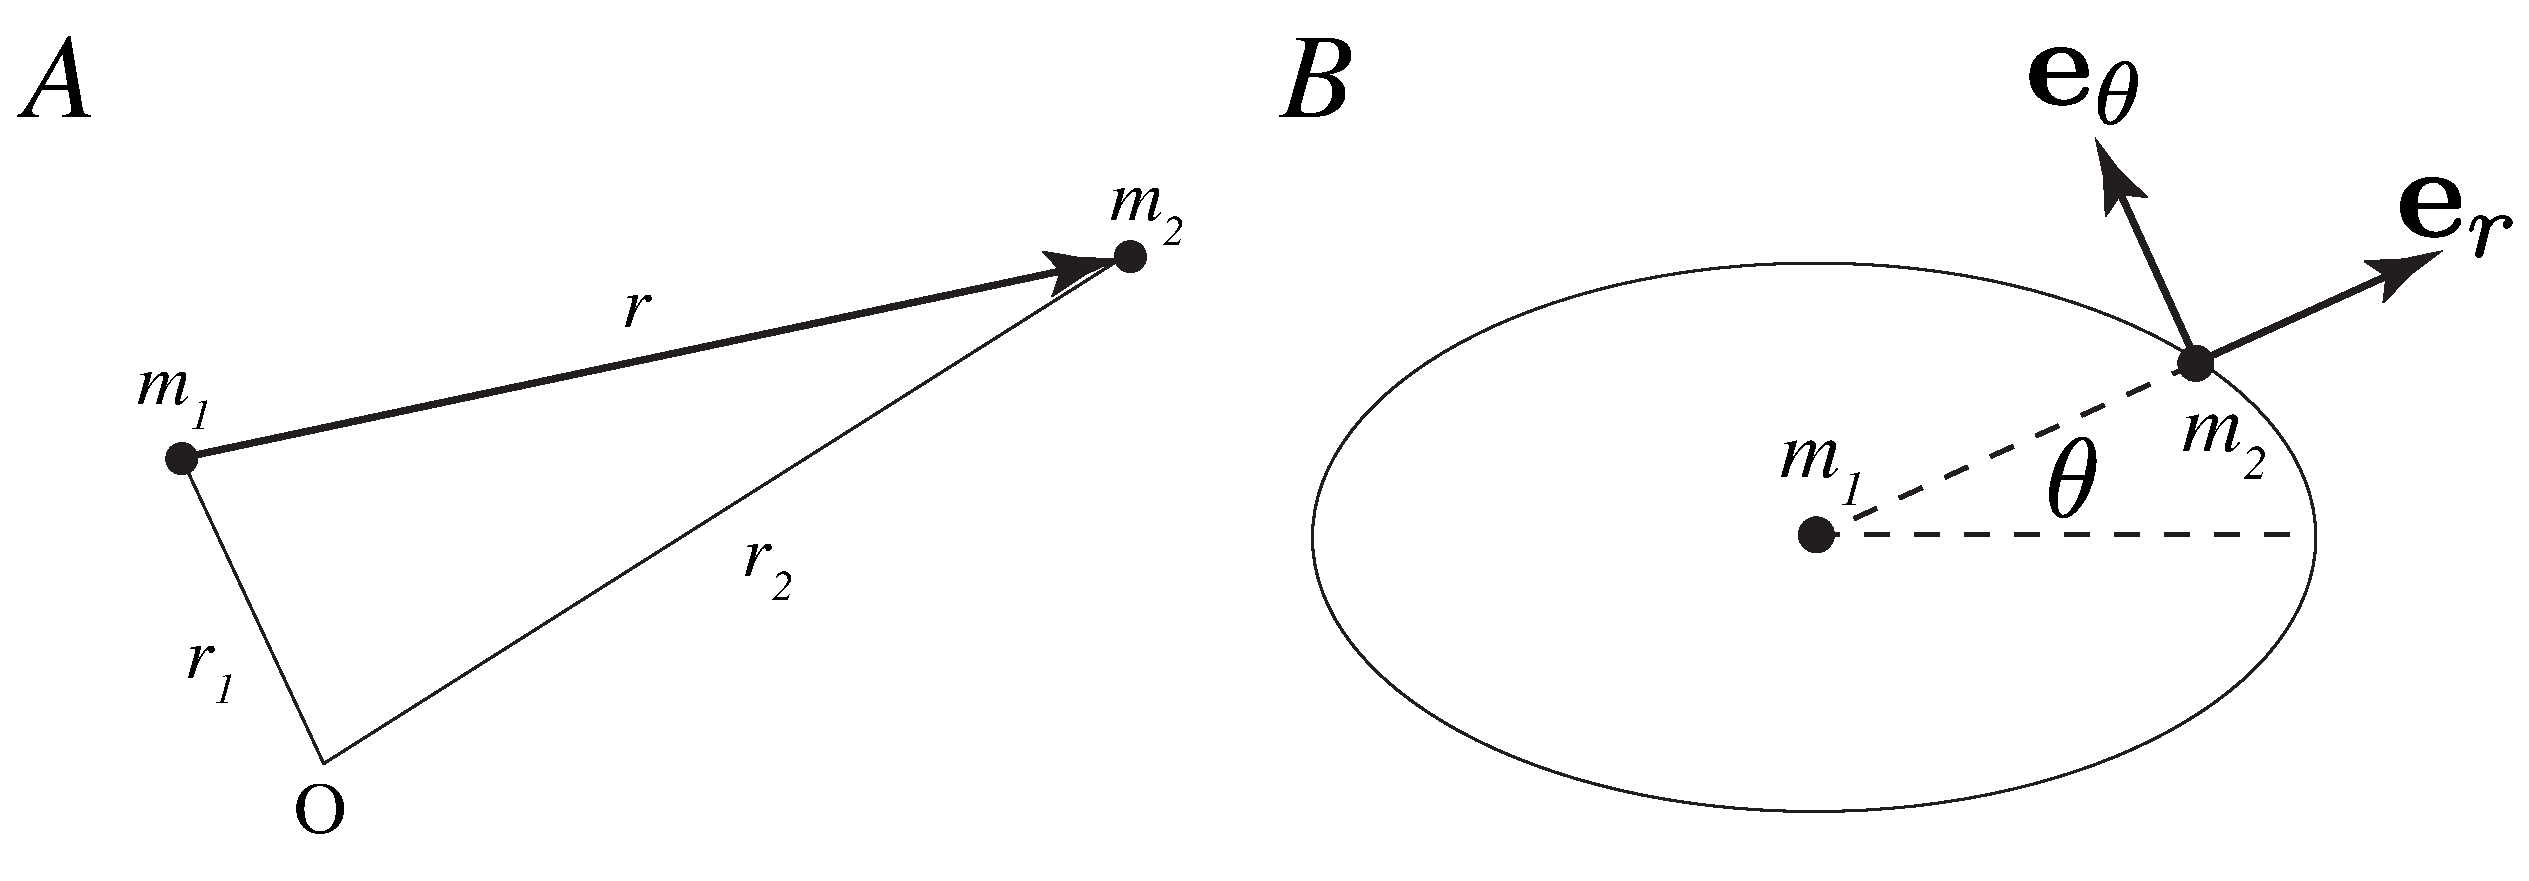
\includegraphics[width=\linewidth]{fig/zahyou.eps}
\end{center}
	\caption{座標系}
	\label{fig:zahyou}
\end{figure} 


\color{red}
\begin{itembox}{問題}
\footnotesize
\color{gray}
ラグランジュ方程式
\begin{align}
\frac{d}{dt} \left( \frac{\partial L}{\partial \dot{r}}\right) - \frac{\partial L}{\partial r} = 0, \,\,\,
\frac{d}{dt} \left( \frac{\partial L}{\partial \dot{\theta}}\right) - \frac{\partial L}{\partial \theta} &= 0
\end{align}
から

\begin{align}
\label{eq:eqrad}
 \ddot{r} - r \dot{\theta}^2 = - \frac{G (m_1+m_2)}{r^2}
\end{align}
と
$
\dot{\bf h} =  0
$
が得られることを確かめよ。ただし
$
{\bf h} \equiv {\bf r} \times \dot{\bf r} 
$
は軌道角運動ベクトルである。

すなわち軌道角運動量ベクトル${\bf h}$は、二体問題上は保存量である。これは質点が${\bf h}$に直交する平面(軌道面\index{きどうめん@軌道面})上の運動に制約されていることを意味する。
\end{itembox}
\color{black}



式(\ref{eq:eqrad})を変数変換し、$u \equiv 1/r$とする。$h u^2 = \dot{\theta}$、$\dfrac{d r}{d t} = \dfrac{d r}{d \theta} h u^2 = - h \dfrac{d u}{d \theta}$を用いて、
\begin{align}
\frac{d^2 u}{d \theta^2} + u = \frac{G (m_1 + m_2)}{h^2}
\end{align}
となる。これは非斉次二階微分方程式であり、斉次解は
\begin{align}
u_h = c_1 \cos{\theta} + c_2 \sin{\theta} = C_1 \cos{(\theta - C_2)}
\end{align}
のように書くことができる。非斉次解は明らかに
\begin{align}
u_i = \frac{G (m_1 + m_2)}{h^2}
\end{align}
であり、これらを足しあわせたものが一般解である。$G (m_1 + m_2)/h^2$をくくり出し、積分定数項を$e$, $\omega$とした一般解は
\begin{align}
u = \frac{G (m_1 + m_2)}{h^2} [ 1 + e \cos{(\theta - \omega)}]
\end{align}
とかける。$r=1/u$に戻すと、
\begin{align}
\label{eq:eqkep}
r =  \frac{h^2}{G (m_1 + m_2)} \frac{1}{ 1 + e \cos{(\theta - \omega)}} 
\end{align}

ところで、図\ref{fig:ellip}のような楕円を考えてみよう。楕円なので
\begin{align}
\label{eq:rellp}
r + r^\prime = 2 a
\end{align}
が成り立つ。また座標から
\begin{align}
\label{eq:rellp2}
(r^\prime)^2 &= (x_p + 2 e a )^2 + y_p^2 \nonumber \\
&= (r \cos{\theta} + 2 e a )^2 + (r \sin{\theta})^2
\end{align}
となる。式(\ref{eq:rellp},\ref{eq:rellp2})から$r^\prime$を消去すると、楕円のconic 方程式
\begin{align}
\label{eq:conic_orig}
r =  \frac{a (1-e^2)}{ 1 + e \cos{\theta}} 
\end{align}
が得られる。

\begin{figure}[]
 \begin{center}
	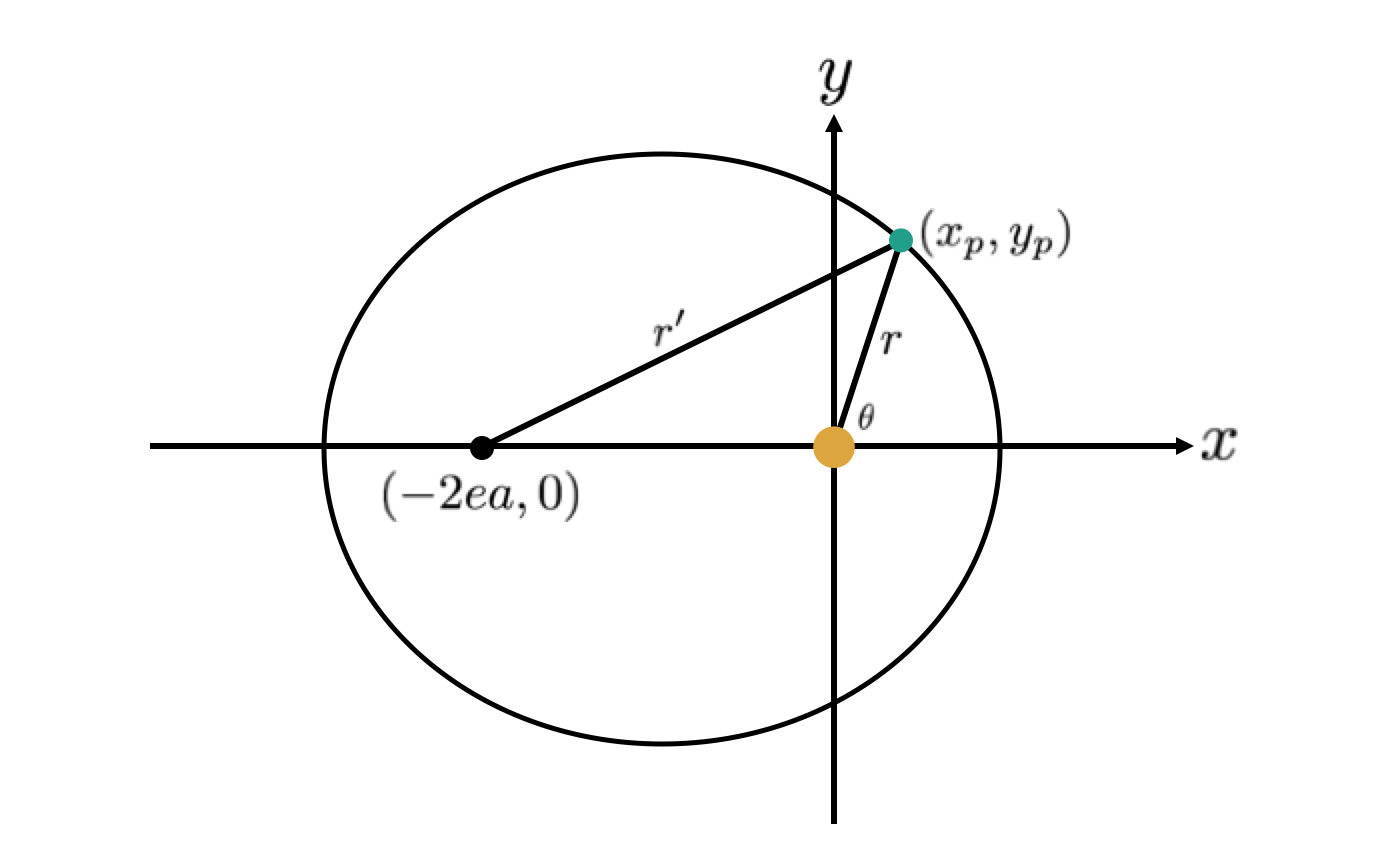
\includegraphics[bb=0 0 695 428,width=1.0\linewidth]{fig/ellip.png}
% 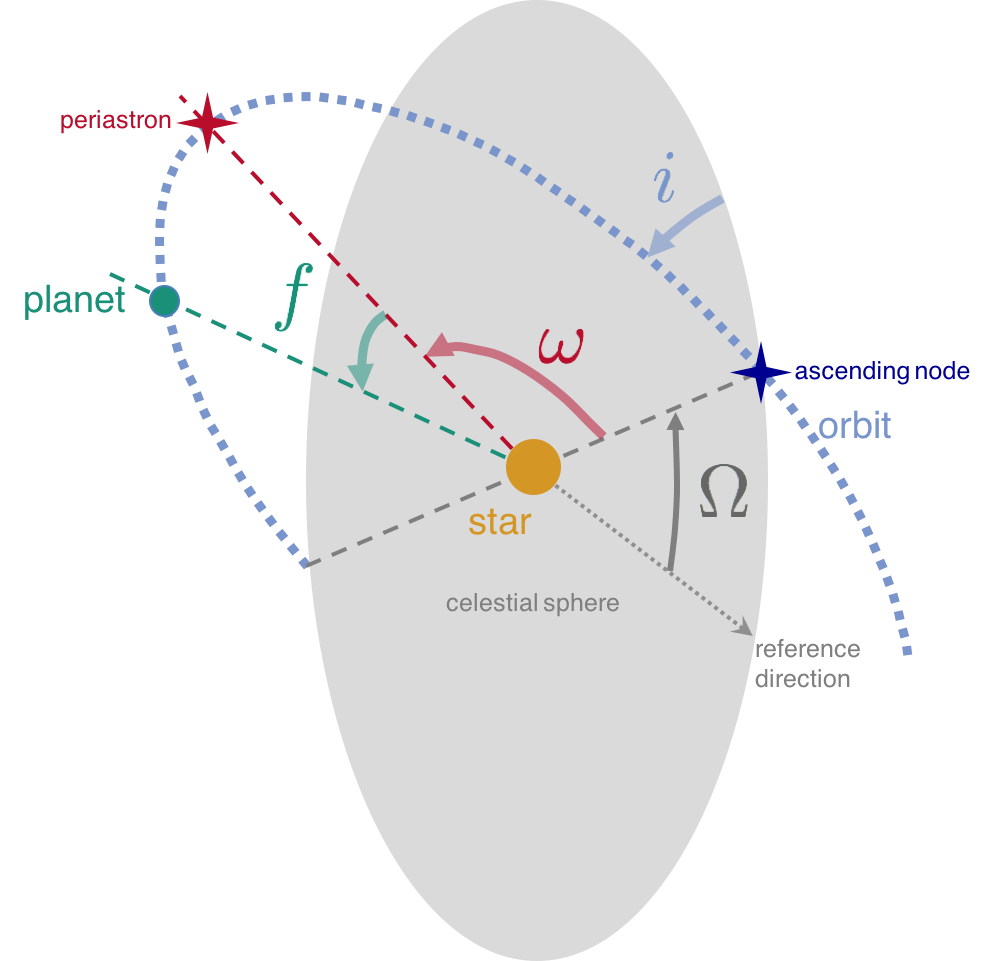
\includegraphics[bb=0 0 474 461,width=1.0\linewidth]{fig/orbele.png}
\end{center}
	\caption{楕円}
	\label{fig:ellip}
\end{figure} 

長半径$a$、短半径$b$、またtrue anomary $f$を
\begin{align}
\label{eq:defkeppar1}
\frac{h^2}{G (m_1 + m_2)} &= a (1 - e^2) \\
\label{eq:defkeppar2}
b^2 &= a^2 (1 - e^2) \\
\label{eq:defkeppar3}
f &\equiv \theta - \omega  
\end{align}
と定義すれば、式(\ref{eq:eqkep})はconic方程式の形
\begin{align}
\label{eq:conic_kepler}
r =  \frac{a (1-e^2)}{ 1 + e \cos{f}} 
\end{align}
になることから、2体問題の解が楕円になることが確認される(ただし$0 \le e < 1$とする)。またtrue anomaly $f$は、periastron(近日点の太陽を恒星に変えたもの)から測った恒星惑星の角度に対応することが分かる。$\omega$はthe argument of periastronと呼ばれる量でconic方程式(\ref{eq:conic_orig})で表される楕円を半時計回りに$\omega$回転したということを表している。

ところで$\dot{A}$は一定であるから楕円面積
\begin{align}
A = \pi a b = \frac{h}{2} P
\end{align}
とかける。ここに$P$は公転周期である。これを変形すると
\begin{align}
\label{eq:kep3}
 P^2 = \frac{4 \pi^2}{G (m_1+m_2)} a^3 
\end{align}
となる。公転周期の自乗は質量に反比例、軌道長半径の3乗に比例することが分かる(ケプラーの第三法則)。円軌道の場合、公転角速度は$1/\sqrt{G (m_1+m_2) a}$であることも分かる。式(\ref{eq:defkeppar1})を用いて$G$を消すことで角運動量表記
\begin{align}
\label{eq:kep3_1}
 P = \frac{2 \pi a^2 \sqrt{1-e^2}}{h} 
\end{align}
もえられる。

\begin{figure}[]
 \begin{center}
%	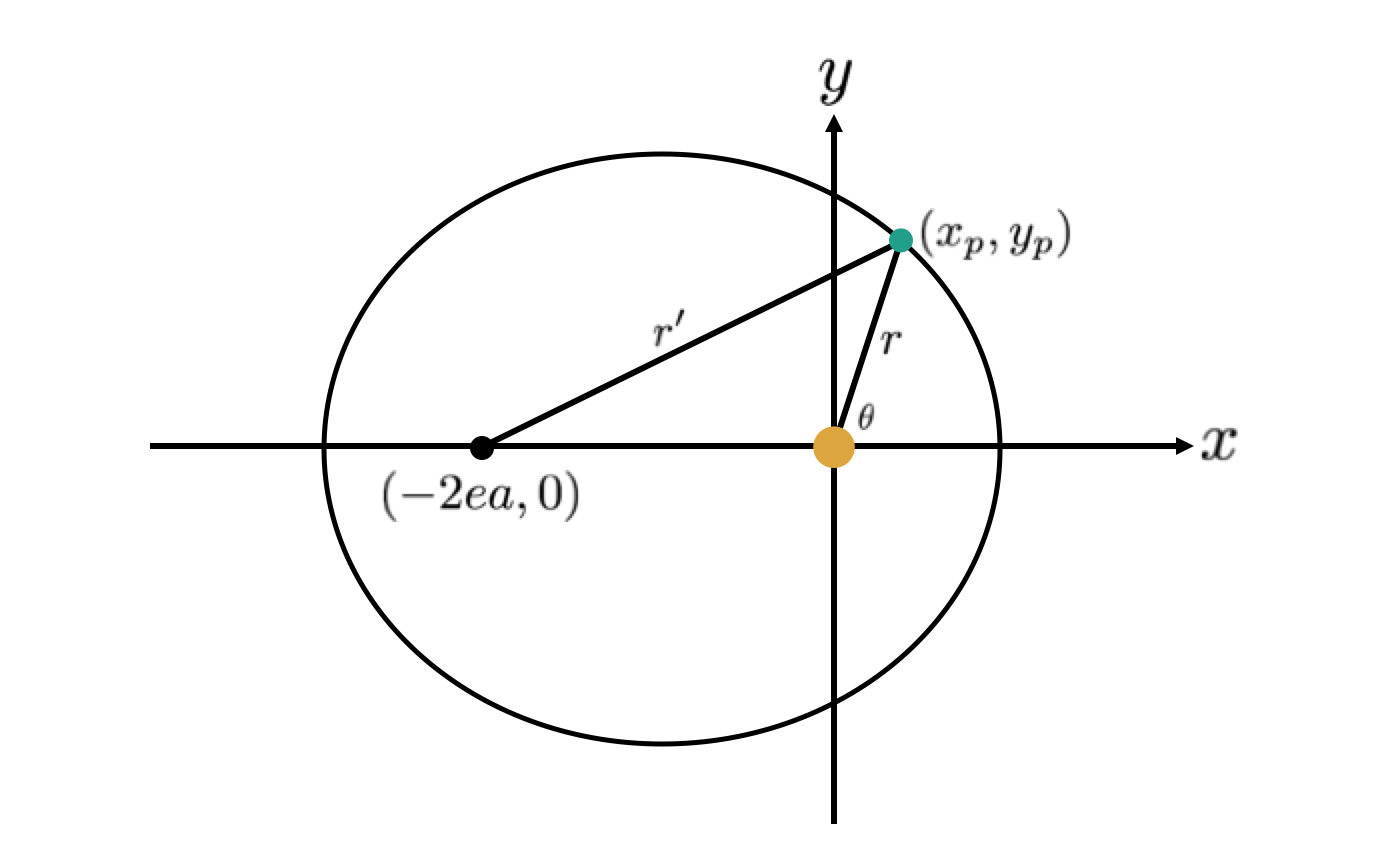
\includegraphics[bb=0 0 695 428,width=1.0\linewidth]{fig/ellip.png}
 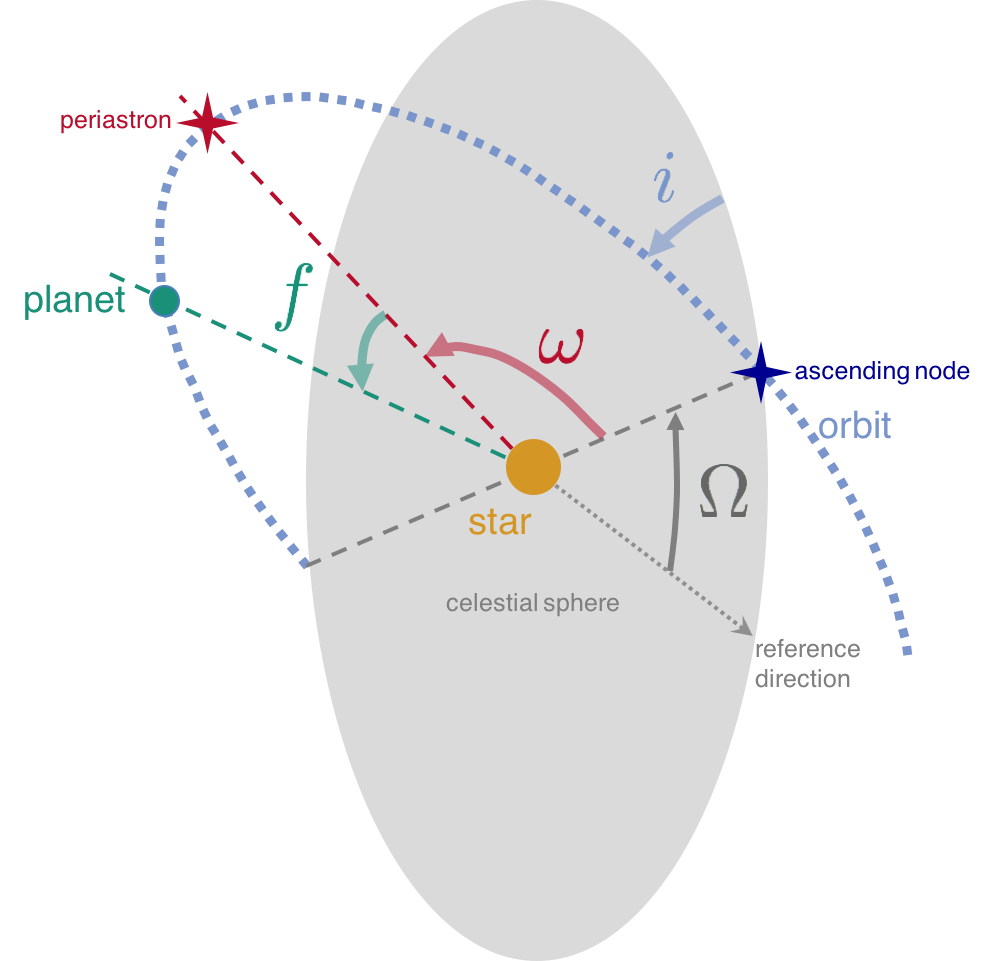
\includegraphics[bb=0 0 474 461,width=1.0\linewidth]{fig/orbele.png}
\end{center}
	\caption{座標系}
	\label{fig:ellip}
\end{figure} 

平均運動は
\begin{align}
    n \equiv \frac{2 \pi}{P}
\end{align}
で定義される。式(\ref{eq:kep3_1})を用いることで
\begin{align}
\label{eq:mean_motion}
    n = \frac{h}{a^2 \sqrt{1-e^2}}
\end{align}
とも表せる。

\section{三次元空間における二体問題 \label{ss:threedtwobody}}

前章では、二次元平面上での二体運動を考えた。実際の天体は観測者から見て三次元空間上に存在しているので、軌道を3次元回転する必要がある。
観測者からみた傾きである軌道傾斜角(orbital inclination)を$i$で、azimuth方向の定義をlongitude of ascending node $\Omega$で指定する。これら$a,e,\omega, f, i, \Omega$の六つのパラメタを指定すれば、三次元空間における二体問題の軌道が一意に決定される。

これらの回転を回転行列で表してみよう。まず、元となる楕円はconic方程式(\ref{eq:conic_orig})であらわされる図\ref{fig:ellip}のものとしよう。$z$軸を紙面に垂直にとるとする。
\begin{itemize}
\item (1) conic方程式(\ref{eq:conic_orig})を$z$軸周りに反時計回りに$\omega$回したものが二体問題の楕円の方程式(\ref{eq:conic_kepler})であった。
\item (2) 次に$x$軸周りに反時計方向に$i$回すと軌道面が天球に対して$i$傾く事になる。\\
\item (3) 最後に$z$軸周りに$\Omega$、つまり天球のazimuth方向の回転の自由度が残る。
\end{itemize}

これらの回転行列を順に楕円を表す$\rv = (r \cos{\theta}, r \sin{\theta},0)$に対してかける。まず(1)は
% ---- 1. position in the orbital plane ---------------------------------
\begin{align}
\rv &=
\begin{pmatrix}
r\cos\theta\\
r\sin\theta\\
0
\end{pmatrix}
=
\begin{pmatrix}
r\cos\!\bigl(f+\omega\bigr)\\
r\sin\!\bigl(f+\omega\bigr)\\
0
\end{pmatrix}
\end{align}
である。次に(2)は
% ---- 2. rotation by the inclination i (about the x-axis) --------------
\begin{align}
\rv^\prime &=
\begin{pmatrix}
1 & 0        & 0\\
0 & \cos i   & -\sin i\\
0 & \sin i   &  \cos i
\end{pmatrix}
\rv \\
&=
\begin{pmatrix}
r\cos\!\bigl(f+\omega\bigr)\\
r\sin\!\bigl(f+\omega\bigr)\cos i\\
r\sin\!\bigl(f+\omega\bigr)\sin i
\end{pmatrix}
\end{align}
となる。
% ---- 3. rotation by the longitude of ascending node Ω (about the z-axis)
最後に(3)は
\begin{align}
\rv^{\prime\prime} &=
\begin{pmatrix}
\cos\Omega & -\sin\Omega & 0\\
\sin\Omega &  \cos\Omega & 0\\
0          &  0          & 1
\end{pmatrix}
\rv^\prime \\
&=
\begin{pmatrix}
r\cos\!\bigl(f+\omega\bigr)\cos\Omega
 - r\sin\!\bigl(f+\omega\bigr)\cos i\,\sin\Omega\\[4pt]
r\cos\!\bigl(f+\omega\bigr)\sin\Omega
 + r\sin\!\bigl(f+\omega\bigr)\cos i\,\cos\Omega\\[4pt]
r\sin\!\bigl(f+\omega\bigr)\sin i
\end{pmatrix}
\\
\label{eq:threed}
&\equiv
\begin{pmatrix}
X\\[2pt] Y\\[2pt] Z
\end{pmatrix}.
\end{align}
となり、三次元空間での軌道$(X,Y,Z)$が得られた。

\section{二体問題を時間について求める}
二体問題の解はtrue anomaly $f$の関数、つまり$r = r(f)$として書かれていた。しかし現実の観測では、二体問題はなんであれ時間の関数として観測される。そこで時間表記$r = r(t)$をどのように求めるか考えてみよう。

方針は以下のとおりである。まず
\begin{align}
        v^2 &= \dot{\rv} \cdot \dot{\rv} 
        = (\dot{r} {\ev}_r + r \dot{f} {\ev}_\theta) \cdot (\dot{r} {\ev}_r + r \dot{f} {\ev}_\theta) \nonumber \\
        \label{eq:v2_1}
        &= \dot{r}^2 + r^2 \dot{f}^2 \\
        \label{eq:v2_2}
        &=  \dot{r}^2 + \frac{h^2}{r^2} 
\end{align}
を考える($h = r^2 \dot{f}$を用いた)。そして、
\begin{itemize}
    \item (1) $v^2$を式(\ref{eq:v2_2})から$r$,$\dot{r}$を$f$の関数に変換し$v^2 (f)$で表す
    \item (2) $v^2(f)$をConic方程式で$v^2(r)$に変換
    \item (3) $v^2 = \dot{r}^2 + h^2/r^2$と等置して$r, \dot{r}$の式、つまり$r$の時間に関する微分方程式を得る
\end{itemize}

(1)について$r$から$f$への変換はConic方程式(\ref{eq:conic_kepler})を用いればよい。また$\dot{r}$を$f$に変換するには
\begin{align}
\label{eq:dotr}
\dot{r} &= \frac{h}{a(1-e^{2})}\,e\sin f 
\end{align}
を用いる。

\begin{itembox}{$\clubsuit$式(\ref{eq:dotr})の導出}
\footnotesize
\color{gray}
\begin{align}
    \dot r
  &=\frac{df}{dt}
   \,\frac{d}{df}\!
     \left(
       \frac{a(1-e^{2})}{1+e\cos f}
     \right)
  =\dot f\,
    \frac{a(1-e^{2})\,e\sin f}{\bigl(1+e\cos f\bigr)^{2}}
    \nonumber \\
    &= \dot{f} \frac{a (1-e^2)}{1 + e \cos{f}} \frac{e \sin{f}}{1 + e \cos{f}} = r \dot{f} \frac{e \sin{f}}{1 + e \cos{f}} \nonumber\\
&= \frac{h}{r} \frac{e \sin{f}}{1 + e \cos{f}}
= \frac{h}{a(1-e^{2})}\,e\sin f
\end{align}
\end{itembox}

つまり
\begin{align}
    v^2 &= \dot{r}^2 + (r \dot{f})^2 = \dot{r}^2 + \frac{h^2}{r^2} \nonumber \\
    &= \frac{h^2}{a^2(1-e^2)^2} [2 (1 + e\cos{f}) + e^2 - 1 ] = v^2(f)
\end{align}



次に$v^2(f)$を再度Conic方程式を用いて$r$の関数に変換する(2)の手順は、
\begin{align}
    v^2(r) &= \frac{h^2}{a (1 - e^2)} \left( \frac{2}{r} - \frac{1}{a} \right)
\end{align}
となる。(3)より$r$の時間微分方程式
\begin{align}
\label{eq:rde}
    \dot{r}^2 - \frac{h^2}{a (1-e^2)}  \left( \frac{2}{r} - \frac{1}{a} \right) + \frac{h^2}{r^2} = 0
\end{align}
を得る。この方程式はそのまま解くことはできない。そこでeccentric anomaly $E$を導入する。
\begin{align}
\label{eq:eanomaly}
    r = a (1 - e \cos{E})
\end{align}
この$E$を用いて、微分方程式(\ref{eq:rde})を$E$, $\dot{E}$の微分方程式に変換すると
\begin{align}
\label{eq:dee}
    \dot{E} = \frac{n}{1 - e \cos{E}}
\end{align}
また、天下りであるが、この解は
\begin{align}
    E - e \sin{E} = n (t -t_0)
\end{align}
で与えられる(微分することで式(\ref{eq:dee})が成り立つことを確かめよ)。ここで時間変数の代理としてMean anomaly $M$を
\begin{align}
    M \equiv n (t - t_0)
\end{align}
と定義することにより
\begin{align}
\label{eq:dee_sol_M}
    f(E) = E - e \sin{E} - M = 0
\end{align}
を解くことで$E$が求まる。

\begin{itembox}{$\clubsuit$式(\ref{eq:dee})の導出}
\footnotesize
\color{gray}
\begin{align}
  \frac{2}{r}-\frac{1}{a}
    &=\frac{1}{a}\!\left(\frac{2}{1-e\cos E}-1\right)     \nonumber \\
    &=\frac{1}{a}\,\frac{1+e\cos E}{1-e\cos E}
      \;=\;
      \frac{1}{a}\,
      \frac{1-e^{2}\cos^{2}E}{(1-e\cos E)^{2}}\;.
\end{align}

\begin{align}
 &\frac{h^{2}}{r^{2}}
 -\frac{h^{2}}{a^{2}(1-e^{2})}\!
  \left(\frac{2}{r}-\frac{1}{a}\right) \nonumber \\
 &= \frac{h^{2}}{a^{2}(1-e\cos E)^{2}}
    -\frac{h^{2}(1-e^{2})}{a^{2}(1-e\cos E)^{2}(1-e^{2})} \nonumber \\
 &=\frac{h^{2}(1-e^{2})}{a^{2}(1-e\cos E)^{2}(1-e^{2})} -\frac{h^{2}(1-e^{2}\cos^{2}E)}{a^{2}(1-e\cos E)^{2}(1-e^{2})}\nonumber \\
 &= -\frac{h^{2}e^{2}\bigl(1-\cos^{2}E\bigr)}
        {a^{2}(1-e\cos E)^{2}(1-e^{2})}
\end{align}

\begin{align}
     \dot r &=\frac{dE}{dt}\,
         \frac{d}{dE}\bigl(a(1-e\cos E)\bigr)
     =\dot E\,a e\sin E \\
  \dot r^{2}
    &=\dot E^{2}\,a^{2}e^{2}\sin^{2}E
\end{align}
これらの式より、
\begin{align}
    \dot E^{2}\,a^{2}e^{2}\bigl(1-\cos^{2}E\bigr)
  =
  \frac{h^{2}\,e^{2}\bigl(1-\cos^{2}E\bigr)}
       {a^{2}(1-e\cos E)^{2}(1-e^{2})}
\end{align}
つまり
\begin{align}
    \dot E^{2}
   =\frac{h^{2}}
          {a^{4}(1-e\cos E)^{2}(1-e^{2})}
\end{align}
$\dot{E} > 0$に軸を取るとすると、
\begin{align}
    \dot E
 &=\frac{h}{a^{2}\sqrt{1-e^{2}}\,(1-e\cos E)} \\
 & = \frac{n}{1 - e \cos{E}}
\end{align}
を得た。最後の変形は平均運動(\ref{eq:mean_motion})を用いた。
\end{itembox}

また$E$と$f$の関係は式(\ref{eq:eanomaly})と二体問題の円錐方程式(\ref{eq:conic_kepler})から
\begin{align}
\label{eq:Efrel}
\cos{f} = \frac{\cos{E} - e}{1 - e \cos{E}}
\end{align}

これにより、周期$P$とオフセット$t_0$が分かれば時間$t$からmean anomaly $M$か計算でき、数値計算で式(\ref{eq:dee_sol_M})を解くことで$E$が、さらに式(\ref{eq:Efrel})からtrue anomaly $f$を求めることができる。\\

\subsubsection{Newton-Raphson法により式(\ref{eq:dee_sol_M})を解く}

非線形方程式$f(E)=0$は数値的に求めることが必要である。このための方法の一つとしてNewton-Raphson法を紹介する。Newton-Raphson法は図\ref{fig:newton_raphson}にしめすように、まず初期値$E_1$から初めて、$f(E_1)$に接する直線を求め、その直線と原点との交点を解析的に求め$E_2$とする。この手続きを$n$回繰り返すという手順である。$i$番目の手続きでは接線(つまり$f(E)$を$E_i$でテイラー展開した一次の項までの近似式)は
\begin{align}
\label{eq:nrm}
   y = f(E_i) + f^\prime(E_i) (E - E_i) 
\end{align}
となることから
\begin{align}
\label{eq:update_newton}
    E_{i+1} &= E_i + \Delta E_i \\
    \Delta E_i &\equiv - \frac{f(E_i)}{f^\prime(E_i)}
\end{align}
となる。$\Delta E_i$を$i$番目の更新項(update term)とよぶ\footnote{単に$f(E)$をテイラー展開して1次まで残した近似を用いて解を更新していくとみることもできる。すなわち
\begin{align}
\label{eq:nrm_f}
   f(E) \approx f(E_i) + f^\prime(E_i) (E - E_i) = 0
\end{align}
の解を$E_{i+1}$として、繰りかえすことに対応している。}。この手続きを収束条件の判定値を$\epsilon$として$ |E_{i+1} - E_{i}| < \epsilon$となるまで繰り返し、条件を満たした$E_i$を近似解とすればよい。

式(\ref{eq:nrm})の計算には$f$の微分が必要である。式(\ref{eq:dee_sol_M})より
\begin{align}
    f^\prime(E) = 1 - e \cos{E}
\end{align}
である。

\begin{figure}[]
 \begin{center}
 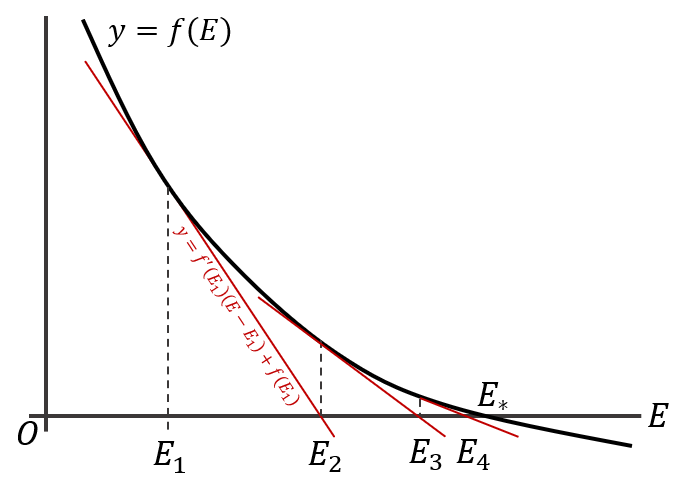
\includegraphics[width=1.0\linewidth]{fig/newton_raphthon.png}
\end{center}
	\caption{Newton-Raphson法の概念図。}
	\label{fig:newton_raphson}
\end{figure} 

\begin{itembox}{二次最適化としてのNewton法$^\dagger$}
\footnotesize
\color{gray}
コスト関数$Q(x)$を最小にする$x=x^\ast$を求める最適化問題
\begin{equation}
   x^\ast = \mathrm{minimize}_{x} \,\, Q(x)  
\end{equation}
の解法として、停留点条件
$d Q(x)/d x = 0$
をNewton-Raphson法で求めることができる。この場合、
$f (x) = Q^\prime (x)$
として、式(\ref{eq:update_newton})を用いると、更新式は
\begin{align}
x_{i+1} &= x_i + \Delta x_i \\ 
\Delta x_i &\equiv - \frac{Q^\prime (x_i)}{Q^{\prime\prime}(x_i)}  
\end{align}
となり、$Q(x)$の二回微分が必要であることから、二次の最適化と呼ばれる。ちなみに最適化の文脈ではRaphsonが省略され、単にNewton法と呼ばれることが多い。

一般に多次元のNewton法も同様に構成できる。多次元のテイラー展開より
\begin{align}
\fv(\xv) \approx \fv(\xv_i) + \Jv (\xv_i) (\xv - \xv_i) = \boldsymbol{0}
\end{align}
をみたす$\xv$が次の更新点となるので、
\begin{align}
    \xv_{i+1} &= \xv_{i} + \Delta \xv_i \\
    \label{eq:second_newton}
    \Delta \xv_i &\equiv - \Jv^{-1} (\xv_i) \fv(\xv_i)
\end{align}
となる。ただし$\Jv (\xv_i)$はヤコビアンである。
\end{itembox}



\section{視線速度}

太陽系外惑星は、惑星の公転による恒星の視線速度方向の変化を、恒星スペクトルのドップラーシフトを通じて検出することで初検出された。

\begin{figure}[]
 \begin{center}
	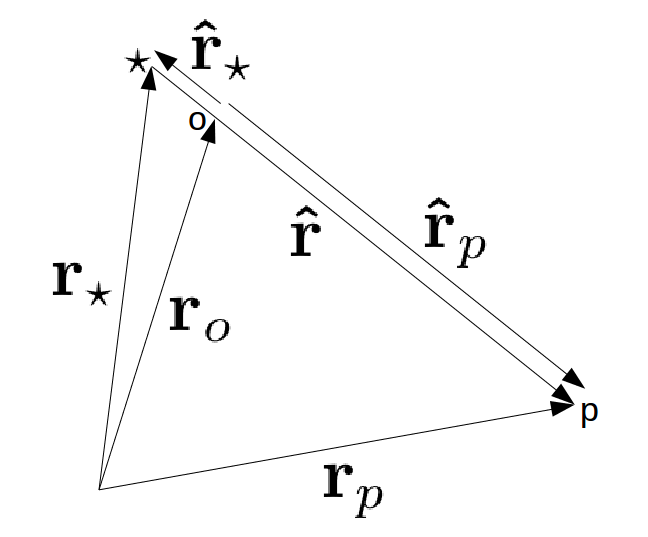
\includegraphics[bb=0 0 648 537,width=1.0\linewidth]{fig/rvector.png}
\end{center}
	\caption{重心$o$と各ベクトルの定義。\label{fig:rvector}}
\end{figure} 

惑星による恒星の視線速度変動を考える。二体の場合、恒星の視線速度は恒星と惑星の重心から測ったベクトルの運動の視線速度が観測される。そこで、図\ref{fig:rvector}のように惑星$p$、恒星$\star$とその重心$o$をおく。主星、惑星質量をそれぞれ$M_\star$、$M_p$とし、主星と惑星の位置を${\bf r}_\star$, ${\bf r}_p$とする。この系の重心${\bf r}_o$は
\begin{eqnarray}
{\bf r}_o = \frac{M_\star {\bf r}_\star+ M_p {\bf r}_p}{M_\star + M_p}
\label{eq:rbary}
\end{eqnarray}
である。重心から測った主星と惑星の位置${\bf \hat{r}}_\star = {\bf r}_\star - {\bf r}_o$, ${\bf \hat{r}}_p = {\bf r}_p - {\bf r}_o$、また主星から惑星に向かうベクトルを${\bf \hat{r}} = {\bf \hat{r}}_p - {\bf \hat{r}}_\star $と定義する。
\begin{align}
\label{eq:barycentsp}
M_\star {\bf \hat{r}}_\star + M_p {\bf \hat{r}}_p &= M_\star {\bf \hat{r}}_\star + M_p ({\bf \hat{r}}_\star + {\bf \hat{r}} ) = 0 
\end{align}
であるから
\begin{eqnarray}
\label{eq:relpossp}
{\bf \hat{r}}_\star = - \frac{M_p}{M_\star + M_p} {\bf \hat{r}}
\end{eqnarray}
である。


まず、観測者から恒星への位置ベクトルは重心までの位置ベクトル${\bf r}_o$を用いて
\begin{eqnarray}
{\bf r}_\star = {\bf r}_o + {\bf \hat{r}}_\star 
\end{eqnarray}
である。{ 恒星は惑星と反対に動くので、視線方向を$Z$軸の反対向きにとり、半時計回りを保つために$\Omega=\pi$ととるとしよう。この場合、} 恒星の視線速度はこの時間微分の$Z$方向への単位ベクトル${\bf e}_Z$と内積をとったもの{ を符号反転させたもの}だから、
\begin{eqnarray}
\label{eq:vrsatare}
v_r = V_\mathrm{sys} { -} \dot{\hat{\bf r}}_\star \cdot {\bf e}_Z
\end{eqnarray}
ここに$V_\mathrm{sys} \equiv { - } \dot{{\bf r}}_o \cdot {\bf e}_Z $は系全体の視線速度である。式(\ref{eq:relpossp})より、
\begin{eqnarray}
\label{eq:vrsatare2}
v_r = V_\mathrm{sys} + \frac{M_p}{M_\star + M_p} \dot{\hat{\bf r}} \cdot {\bf e}_Z
\end{eqnarray}
と変形できる。この${\bf \hat{r}}$は、二体問題の${\bf r}$に対応させれば、そのまま定式化を用いる事ができる。すると$\dot{\hat{\bf r}}_\star \cdot {\bf e}_Z$は、三次元座標系の$Z$成分の時間微分$\dot{Z}$に対応する事になる。すなわち式(\ref{eq:threed})を用いて
\begin{eqnarray}
\label{eq:vrsatare3}
v_r &=& V_\mathrm{sys} + \frac{M_p}{M_\star + M_p} \dot{Z} 
\end{eqnarray}
となる。
\begin{align}
\dot{Z} &= \frac{d}{d t} \left[ r \sin{i} \sin{(f + \omega)} \right] \nonumber \\
&= \dot{r} \sin{i} \sin{(f + \omega)} + r \dot{f} \sin{i} \cos{(f + \omega)}
\end{align}
である。

式(\ref{eq:dotr})と$r \dot{f} = h/r$とConic方程式(\ref{eq:conic_kepler})をもちいて、
\begin{align}
\label{eq:vrsatare4}
&v_r =V_\mathrm{sys} + \frac{M_p}{M_\star + M_p} \frac{h \sin{i}}{a (1-e^2)} [ e \sin{f} \sin{(f+\omega)}   \nonumber \\
&+ e \cos{f} \cos{(f+\omega)} + \cos{(f+\omega)} ] \\
&=V_\mathrm{sys} + \frac{M_p}{M_\star + M_p} \frac{h \sin{i}}{a (1-e^2)} \left[ \cos{(f+\omega)} + e \cos{\omega} \right] \nonumber \\
\end{align}
となる。
\begin{itembox}{$\clubsuit$}
\footnotesize
\color{gray}
$\sin{f} \sin{(f+\omega)} + \cos{f} \cos{(f+\omega)} = \cos{(-f)} \cos{(f+\omega)} - \sin{(-f)} \sin{(f+\omega)} = \cos{(-f + f + \omega)} = \cos{\omega}$
\end{itembox}

もしくは$h$を陽に書き下すと
\begin{align}
\label{eq:vrsatarefinal}
v_r &= V_\mathrm{sys} + K_\star \left[ \cos{(f+\omega)} + e \cos{\omega} \right] \\
\label{eq:vrKrv}
K_\star &\equiv \frac{M_p \sin{i}}{\sqrt{1 - e^2}} \sqrt{\frac{G}{(M_p + M_\star) a}} 
\end{align}
が二体問題の視線速度カーブとなる。また視線速度変動のオーダーは
\begin{align}
K_\star &\sim 30 \mathrm{m/s} \, \frac{M_p \sin{i}}{M_J}\left(\frac{M_\star}{M_\odot} \right)^{-1/2} \left(\frac{a}{\mathrm{au}} \right)^{-1/2} \\
&= 130 \mathrm{m/s} \, \frac{M_p \sin{i}}{M_\oplus}\left(\frac{M_\star}{M_\odot} \right)^{-1/2} \left(\frac{a}{0.05 \mathrm{au}} \right)^{-1/2} \mbox{(HJ)} \nonumber \\
&= 0.1 \mathrm{m/s} \, \frac{M_p \sin{i}}{M_\oplus}\left(\frac{M_\star}{M_\odot} \right)^{-1/2} \left(\frac{a}{\mathrm{au}} \right)^{-1/2}  \mbox{(Earth)} \nonumber 
\end{align}
となる。また、この視線速度変動に対応するドップラーシフトは
\begin{align}
    \frac{\Delta \lambda}{\lambda} &\sim \frac{K_\star}{c} \nonumber \\
    & = 10^{-7} \frac{M_p \sin{i}}{M_J}  \left(\frac{M_\star}{M_\odot} \right)^{-1/2} \left(\frac{a}{\mathrm{au}} \right)^{-1/2}
\end{align}
となる。現在の高分散分光器の分解能は$R \sim 10^5$であるので、多数の分子吸収線(と光子数)をもちいてS/Nをブーストすることが重要となる。またプラクティカルには、ヨードセルや周波数コムを用いた波長較正の安定化が重要である。


\begin{itembox}{$\clubsuit$}
%\tiny
\footnotesize
\color{gray}
\begin{align}
    K_\star &\sim \frac{M_p \sin{i}}{M_\odot}\left(\frac{M_\star}{M_\odot} \right)^{-1/2}  \sqrt{ \frac{G M_\odot}{a} } \nonumber \\
    &= \frac{M_p \sin{i}}{M_\odot}\left(\frac{M_\star}{M_\odot} \right)^{-1/2} \sqrt{ \frac{2 G M_\odot}{c^2}\frac{1}{2a} } \, c \nonumber \\
    &= \frac{M_J}{M_\odot} \frac{M_p \sin{i}}{M_J} \left(\frac{M_\star}{M_\odot} \right)^{-1/2} \sqrt{ \frac{r_g}{2  \mathrm{au}} \frac{\mathrm{au}}{a} }\, c \nonumber \\
    &= 10^{-7} c \frac{M_p \sin{i}}{M_J}  \left(\frac{M_\star}{M_\odot} \right)^{-1/2} \left(\frac{a}{\mathrm{au}} \right)^{-1/2} \nonumber \\
    &= 30 \mathrm{m/s} \, \frac{M_p \sin{i}}{M_J}\left(\frac{M_\star}{M_\odot} \right)^{-1/2} \left(\frac{a}{\mathrm{au}} \right)^{-1/2} \nonumber
\end{align}
\end{itembox}

\subsection*{時間の関数としての視線速度カーブ}

さて、実際の観測では時間の関数として測定値が得られるので、この解を時間の関数で書きたい。時間$t$から周期が分かるとmean anomaly $M$かわかる。$M$からeccentric anomaly $E$ は式(\ref{eq:dee_sol_M})を数値的に解く。
これらにより、式(\ref{eq:vrsatarefinal})を数値的に時間で書きなおす事ができる。このように視線速度カーブから求まる物理量は式(\ref{eq:vrsatarefinal})から$V_\mathrm{sys}, K_\star, e, \omega$である。また$f$に関係して周期$P$と位相量(時刻のオフセット)も推定するパラメタとなる。図\ref{fig:rvsim}は幾つかの視線速度カーブと対応する楕円軌道を書いたものである。ケプラー第二法則より天体が近点付近に来た時に急速に視線速度カーブが変化するのをイメージできるだろう。

\begin{figure}[]
 \begin{center}
	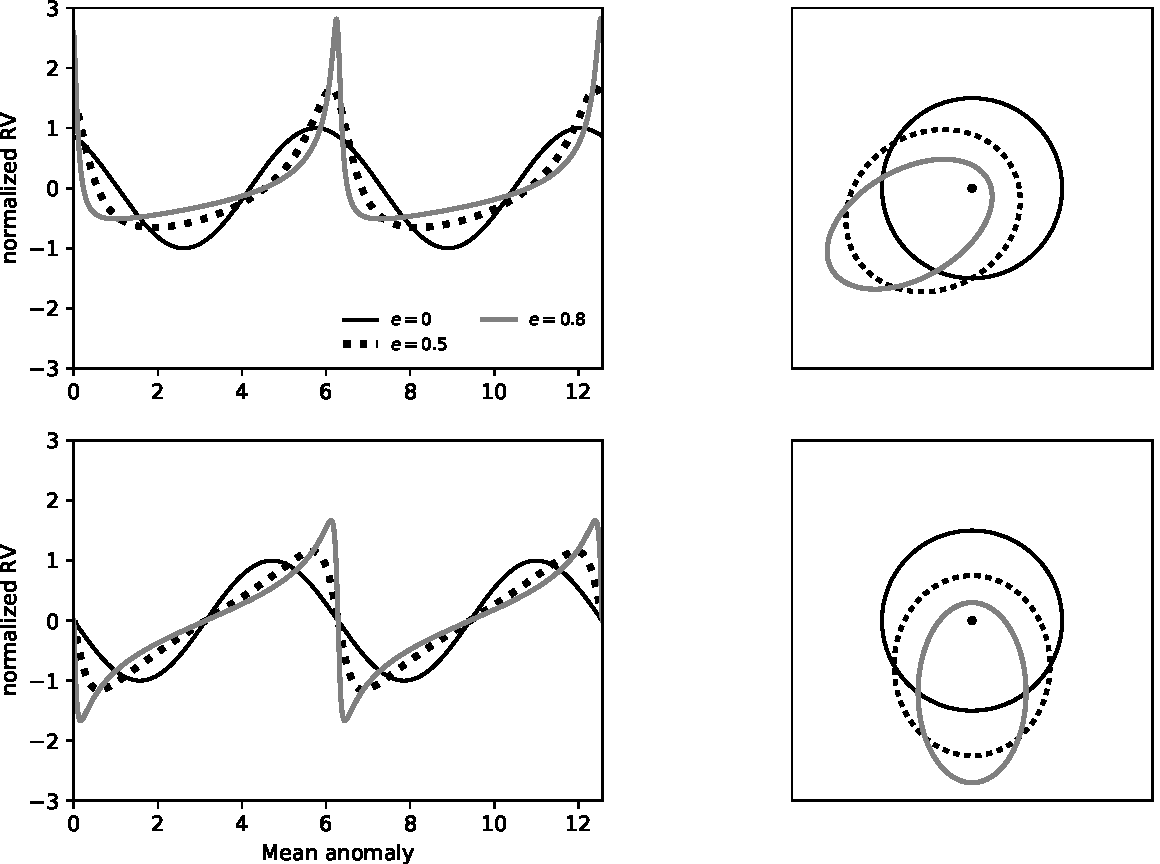
\includegraphics[width=\linewidth]{fig/rvsim.pdf}
\end{center}
	\caption{視線速度カーブ(左)と対応する軌道(右)。上段は$\omega=\pi/6$,下段は$\omega=\pi/2$である。線種は黒実線が$e=0$、黒点線が$e=0.5$、灰色実線が$e=0.8$に対応している。右の楕円は$i=\pi/2$の時に軌道を上から見たものに対応し、下から上むきに視線方向をとると、視線速度カーブの恒星軌道、上から下向きにとると惑星の軌道に対応する。\label{fig:rvsim}}	
\end{figure} 


\begin{itembox}{Binary Mass Function$\,^\dagger$}
%\tiny
\footnotesize
\color{gray}
そもそも視線速度解析は恒星惑星系以前に連星系で発展してきた。この場合、$M_p \ll M_\star$は成り立たない。式(\ref{eq:vrKrv})を、$\star \to 1$と$p \to 2$で書き直し、ケプラー第三法則(\ref{eq:kep3})を用いて、右辺に観測量だけ、左辺に物理パラメタとわけて書くと
\begin{align}
  \label{eq:bmfunc}
  f \equiv \frac{M_2^3}{(M_1 + M_2)^2} \sin^3{i} = \frac{P K_1^3}{2 \pi G} (1 - e^2)^{3/2}
\end{align}
のようになる。この$f$が、一般の質量比の場合、星1の視線速度カーブの観測量$K_1$、$e$、$P$のみからわかる量である。この$f$をbinary mass function\index{Binary Mass Function@Binary Mass Function}と呼ぶ。

また、逆に
\begin{align}
  \label{eq:semiamp2}
  K_1 &= 29.8 \, [\mathrm{km/s}]  \frac{\sin{i}}{\sqrt{1 - e^2}} \left( \frac{M_2}{M_1 + M_2} \right) \nonumber \\
  &\times \left( \frac{M_1 + M_2}{M_\odot} \right)^{1/3} \left( \frac{P}{1 \mathrm{yr}} \right)^{1/3}
\end{align}
とスケーリングされた式を用いると、連星系の場合の検出可能性の見積もりに便利である。この29.8 km/sという値は地球の公転速度に一致している。

\end{itembox}

\section{アストロメトリ}
視線速度変動は3次元ケプラー運動の$\dot{Z}$成分の運動情報を用いていた。アストロメトリは天球上の星の位置を計測する手法であるから、($X$,$Y$)成分の運動情報を用いることになる。固有運動・パララックスを補正後の二体運動による恒星の位置は、観測者から恒星までの距離を$d$として、観測量である角度(離角)としてあらわすと
\begin{align}
   {\boldsymbol{\theta}} = \frac{\hat{\rv}_\star}{d} = - \frac{M_p}{M_\star + M_p} \frac{\hat{\rv}}{d}
\end{align}
に二次元射影となる。すなわち式(\ref{eq:threed})より、
\begin{align}
    \theta_x &= - \frac{M_p}{M_\star + M_p} \frac{X}{d} = - \frac{M_p}{M_\star + M_p} \frac{r}{d} \nonumber\\
    &\times [\cos\!\bigl(f+\omega\bigr)\cos\Omega
 - \sin\!\bigl(f+\omega\bigr)\cos i\,\sin\Omega]\\
     \theta_y &= - \frac{M_p}{M_\star + M_p} \frac{Y}{d} =- \frac{M_p}{M_\star + M_p}\frac{r}{d} \nonumber\\
     &\times [ \cos\!\bigl(f+\omega\bigr)\sin\Omega
 + \sin\!\bigl(f+\omega\bigr)\cos i\,\cos\Omega]
\end{align}
となる。この解は($i \to \pi - i$, $f \to 2 \pi - f$, $\omega \to 2 \pi - \omega$)の変換に不変であり、これはアストロメトリのみでは惑星が近づいているのか遠ざかっているのかはわからない。


\chapter{運動の推定}\label{ch:infer}

第\ref{ch:motion}章では系外惑星の運動に関する観測量の物理モデルを扱った。これらはすべて1次元の時系列データである。本章では一次元の時系列データから、物理モデルと統計モデルを組み合わせることでの内部パラメタである系外惑星の物理量の推定を行う。
観測データ$\dv$と理論モデル$\fv$との比較により以下のようなことが得られる。
\begin{enumerate}
\item ある理論モデル$\fv$は観測データを説明できるモデルかどうか知る 
\item ある理論モデル$\fv$が正しいとしたとき、そのモデル内に含まれるパラメタ$\thetav$をデータ$\dv$にもとづいて決定・推定する ({\bf パラメタ推定})
\item 複数のモデルが存在するときにどちらのモデルが観測$\dv$をよく説明できるか ({\bf モデル選択})
\end{enumerate}
モデル選択はいろいろ大変なので、ここではパラメタ推定について考える。



ここでは例として以下にあげる視線速度の観測データと理論モデルの比較を行う。この場合、$\dv$はrvデータ列を並べたベクトルと考えればよく、各要素$d_i$はこれに対応する時間$t_i$を通じて、理論モデルと比較可能となる。理論モデルは式(\ref{eq:vrsatarefinal})である。パラメタベクトルは$\thetav = (V_\mathrm{sys}, K_\star, e, \omega, T_0, P)$であることがわかる。

\begin{itembox}{視線速度の生データ $\dv$}
\footnotesize
\color{gray}
\href{https://github.com/HajimeKawahara/class25}{https://github.com/HajimeKawahara/class25}
を参照
\end{itembox}


\section{点推定と最適化}
パラメタ$\thetav$を内部に持つモデル$\fv(\thetav)$とデータ $\dv$を何らかの手段で比較することで、一つのパラメタを選択するるパラメタ推定を\underline{点推定}という。もし、データに誤差が全く含まれていなかったら
\begin{align}
    \dv - \fv(\thetav) = \boldsymbol{0}
\end{align}
となる$\thetav$を探せばよいだろう。しかし、通常、データには観測誤差が含まれていて、このような式を満たす$\thetav$は通常見つからない。すなわち
\begin{align}
    \dv = \fv(\thetav^\ast) + \epsilonv
\end{align}
のようにかける。この式は、モデル$\fv$が正しく、かつ"正しい"パラメタ$\theta^\ast$が存在し、残差ベクトル$\epsilonv$が観測誤差のみに由来しているということを含意している。観測誤差を扱う形で理論構成を行うには、観測誤差を生成する確率モデルが必要であることがわかる。たとえば、$\epsilonv$が独立のゼロ平均の正規分布に従うとき、
\begin{align}
 \epsilon_i \sim \mathcal{N}(0,\sigma) 
\end{align}
とかける。もしくはもっと簡潔に物理モデル$\fv(\thetav^\ast)$は確率モデルの平均値であるとして
\begin{align}
    d_i \sim \mathcal{N} (f_i(\thetav^\ast), \sigma)
\end{align}
という理論モデル構成を行うことができる。

さてこの議論でわかるのは、観測データと理論モデルを比較する、といったときの理論モデルとは、$\fv$だけではなく確率モデルも指定しないとならない。図式的に書くと
\begin{itembox}{実証可能な理論モデル}
 実証可能な理論 = 物理・化学モデル + 確率モデル
\end{itembox}

通常、理論天文学では物理・化学モデルを重視しすぎるあまり確率モデルをおろそかにしがちである。また観測天文学では物理・化学モデルを固定しがちである。確率モデルの構成は、実際的な問題として計算量が多く、近年までは簡単には扱えなかった。しかし、最近は計算機の進歩とベイズ統計手法の進歩でこれに対処できるようになってきた。

さて、点推定に戻る。データ間の相関誤差がある場合も多いが、これはガウス過程によるモデリングに譲るとして、今は独立に誤差が入っているとしよう。さらにその誤差がどのデータ点に対しても同じ$\sigma$のガウシアンだとする。この場合、$\thetav$をもつモデル$\fv(\thetav)$が$\dv$を生じさせる確率は
\begin{align}
    p(\dv|\thetav) &= \prod_{i=1}^N \mathcal{N} (f_i(\thetav), \sigma ) \\
    &\propto \exp{\left( - \dfrac{\sum_{i=1}^N (f_i(\thetav) - d_i)^2 }{2 \sigma^2}\right)}
\end{align}
となる。これは尤度関数(likelihood)である。尤度を最も大きくする$\thetav$を点推定値として採用する方法を最尤法という。この場合、
\begin{align}
    \thetav^\ast &= \mathrm{minimize}_{\thetav} \, L_2(\thetav) \\
    L_2(\thetav) &= \sum_{i=1}^N (f_i(\thetav) - d_i)^2 
\end{align}
という最適化問題をとけばよいということになる。
これは最小二乗法そのものである。すなわち最小二乗法は、誤差が独立なガウシアンであると仮定したときの最尤推定と一致する。


最小二乗法による点推定の仮定をもう少しゆるくしたものが、$\chi^2$最小化である。これは、各データ点の$\sigma_i$が既知だとして
\begin{align}
    p(\dv|\thetav) &\propto \exp{\left( - \sum_{i=1}^N \dfrac{ (f_i(\thetav) - d_i)^2 }{2 \sigma_i^2}\right)}
\end{align}
となることより、
\begin{align}
    \thetav^\ast &= \mathrm{minimize}_{\thetav} \, \chi^2(\thetav) \\
    \chi^2(\thetav) &= \sum_{i=1}^N \dfrac{ (f_i(\thetav) - d_i)^2 }{2 \sigma_i^2}
\end{align}
の最適化問題を解くというものである。

\section{最適化問題と自動微分}
さてここまでの議論から、点推定の実際的な問題系は最適化問題であるということがわかる。非線形モデルの最適化問題をとくには、以前見た二次最適化としてのNewton法や、その発展である準ニュートン法、諸先生方がNumerical Recipesを熟読しながら実装したマルカート法、もしくはアメーバー法としてしられる勾配を用いないNelder-Mead法など多種多様な方法がある。

しかしここでは、自動微分を用いた一次の最適化を考える。これはパラメタ数が多いと二次最適化はヘッシアン計算に律速されるためである。そのためニューラルネットなどの機械学習モデルは一次最適化を用いることが多い。一次最適化の基本は最急降下法であり
\begin{eqnarray}
\thetav^{(k)} &=& \displaystyle{\thetav^{(k-1)} - \gamma \frac{\partial}{\partial \thetav} f(\thetav)}
\end{eqnarray}
のように、最も急な坂を下っていく方法である。最急降下法だと行き過ぎることがおおいので、さまざまなモーメントをつけて落ちやすくする。代表的な方法はADAM\cite{kingma2015adam}であるがここではアルゴリズムの詳細には踏み入れない。

\begin{figure}[htb]
\begin{center}
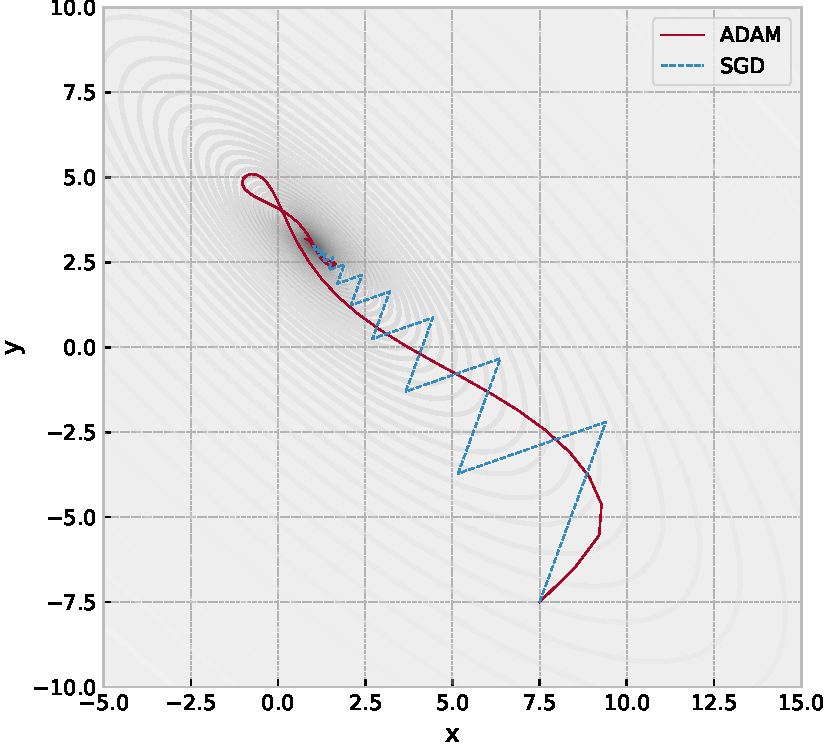
\includegraphics[width=\linewidth]{fig/opt1.pdf}
\caption{一次最適化の例。\label{fig:opt1}}
\end{center}
\end{figure}

一次最適化では、モデルのパラメタによる微分が必要である。数値的に微分値を求めるにはおおまかに4つの方法がある。一つ目は手で微分(manual differentiation)をし、結果をコーディングすることである。これはモデルが複雑になってくると破綻しがちであり、またフレキシビリティの観点からもモデルの継続的な改良を妨げる。次にmathematica等によるsymbolic differentiationを用いて手で微分する代わりに微分結果を得てコーディングすることが考えられる。これはmathematica等を用いたことのある方ならばわかると思うが、モデルが複雑になってくると膨大な項数の結果が排出されるので、やはりフレキシビリティの観点からは難点がある。次に、数値微分を行うことが考えられる。数値微分はモデルが複雑になってくるとエラーがたまりやすい。そこで機械学習分野などで用いられているのが{\sf JAX}/tensorflow/pytorchなどで用いられている、自動微分である。コーディングできるモデルは通常、様々な微分の既知である関数(ここでは要素関数と呼ぼう)の加減乗除の組み合わせでできている。そこで、自動微分では、連鎖則が成り立つように各要素関数
\begin{eqnarray}
x:\to f(x)
\end{eqnarray}
を関数のアウトプットとその微分値の情報
を出力するように拡張する。また微分の加乗除の演算規則がなりたつように演算を定義する。自動微分の実装法としては{\sf JAX}ではJacovian Vector Product (JVP)を用いたものが使用されている。しかしここではイントロダクションとしてより説明が容易な、双対数を用いた方式を使用して自動微分を解説しよう。

双対数(dual number)、$z \in k[\epsilon]/\langle \epsilon^2\rangle$\footnote{多項式環の商環のことをしめしている。詳しくはたとえば雪江明彦「環と体とガロア理論」などを参照。}は$a, b \in \mathbb{R}$にたいし、
\begin{eqnarray}
z &=& a + b \epsilon \\
\epsilon^2 &=& 0
\end{eqnarray}
となる数である。複素数は$i^2 = -1$であったのが$\epsilon^2 = 0$となったと考えればよい。変数$x$の拡張として実部$a$に$x$を、非実部$b$に$x^\prime$を割り当てると、$z = f + f^\prime \epsilon, w = g + g^\prime \epsilon$に対し、可算・乗数・除算はそれぞれ
\begin{eqnarray}
\label{eq:add_ad_dual}
z + w &=& (f + g) + (f^\prime + g^\prime) \epsilon \\ 
\label{eq:mul_ad_dual}
z w &=& f g + (f^\prime g + f g^\prime) \epsilon\\ 
z/w &=& \frac{f}{g} + \frac{f^\prime g - f g^\prime}{g^2} \epsilon
\end{eqnarray}
となる。これは実部に関して通常の、また非実部に関して微分の加乗除則と同じであることを示している。次に連鎖則を実現するには関数$x:\to F(x)$を
\begin{eqnarray}
\label{eq:funcdual}
x+x^\prime \epsilon: \to F(x) + F^\prime(x) x^\prime \epsilon  
\end{eqnarray}
と拡張すればよい。ここで$F(x)$を元の関数、双対数をもつ拡張された関数を$\hat{F}(x+x^\prime \epsilon)$と分けて表記する。すると式(\ref{eq:funcdual})は
\begin{eqnarray}
\label{eq:chain_ad}
\hat{F}(x+x^\prime \epsilon) =  F(x) + F^\prime(x) x^\prime \epsilon
\end{eqnarray}
と書ける。さて連鎖則$G(F(x))$の拡張は
\begin{eqnarray}
\hat{G}(\hat{F}(x+x^\prime \epsilon)) &=&  \hat{G}(F(x) + F^\prime(x) x^\prime \epsilon) \\
&=& G(F(x)) + G^\prime(F(x)) F^\prime(x) x^\prime \epsilon
\end{eqnarray}
となり、実部は通常の合成($G(F(x))$)が、非実部は連鎖則$G^\prime(F(x)) F^\prime(x) x^\prime = \frac{d G}{d F} 
\frac{d F}{d x} x^\prime$が実現されているのが確認できる。

\subsection*{ミニマム自動微分実装}
というわけで小さな自動微分をPythonで実装してみよう。ここで解きたい問題を
\begin{eqnarray}
\label{eq:sample_func}
F(x) = \log{(\cos{x} \sin{x})} + \sin{x}
\end{eqnarray}
の$x=1$で微分 $F^\prime(1)$とする。さらにその合成関数
\begin{align}
\label{eq:dualad2}
G(x) &= F(F(x))
\end{align}
の$x=1$での微分$G^\prime(1)$も求めたい。式(\ref{eq:dualad2})を手で微分するのは大変であるし、symbolic differentiationの結果も長大である。しかし自動微分ならばかなりすっきりしたコードになる。

まず関数(\ref{eq:sample_func})に存在する演算は可算と乗算であるので、式(\ref{eq:add_ad_dual})、(\ref{eq:mul_ad_dual})に対応した双対数の可乗算を定義する。
\begin{minted}[linenos=true, frame=single, numbersep=6pt, mathescape=true]{python}
def mul(x, y):
    a, b = x
    c, d = y
    return a*c, a*d + b*c

def add(x, y):
    a, b = x
    c, d = y
    return a + c, b + d
\end{minted}
ここに$x,y$はそれぞれ双対数である。次に関数(\ref{eq:sample_func})に存在する要素関数は$\sin{x}$、$\cos{x}$、$\log{x}$である。式(\ref{eq:chain_ad})を実装するには、双対数の実部と非実部をペア$(a,b)$の形式であらわすと、関数$F(x)$に対し
\begin{eqnarray}
(x,dx) \to (F(x),F^\prime(x) dx) 
\end{eqnarray}
となるように入出力を与えればよいことがわかる。そこで
\begin{minted}[linenos=true, frame=single, numbersep=6pt, mathescape=true]{python}
import numpy as np
def cos(x):
    a, b = x
    return np.cos(a), - np.sin(a)*b

def sin(x):
    a, b = x
    return np.sin(a), np.cos(a)*b
    
def log(x):
    a, b = x
    return np.log(a), b/a 
\end{minted}
これで終わりである。あとは

\begin{minted}[linenos=true, frame=single, numbersep=6pt, mathescape=true]{python}
f = lambda x: 
add(log(mul(cos(x),sin(x))),sin(x))
df = lambda x: f([x,1.0])
df(1.0)
\end{minted}
とすれば$(F(1), F^\prime(1))$が (0.05324076815279066, -0.37501280285243144)と求まる。$G^\prime(x)$も簡単で、
\begin{minted}[linenos=true, frame=single, numbersep=6pt, mathescape=true]{python}
g = lambda x: f(f(x))
dg = lambda x: g([x,1.0])
dg(1.0)
\end{minted}
とするだけで(-2.8816056725768977, -7.391555094461485)と求まる。以上の例からわかるように自動微分の実際の計算には代数計算を用いているため数値微分に比べて誤差の蓄積は少ない。またフレキシブルにコーディングが可能である。

ここでは自分で実装してみたが、実際にはJAXやpytorch, Enzyme.jlなどの自動微分パッケージを利用することになるだろう。さらに自動微分は、次に示すベイズ統計的なパラメタ推定でも威力を発する。このようにコードをエンドトゥーエンドで微分可能にしておくプログラミングを\underline{微分可能プログラミング}という\cite{2024arXiv240314606B}。
\section{ベイズの定理}

ベイズの定理(Bayes' theorem)とは、事象 $A$ が起こる条件のもとで、別の事象 $B$ が観測される確率を示す定理である。これは条件付き確率に関する基本的な関係式として知られている。

ベイズの定理を数式で表すと、以下のようになるのである。

\[
p(A \mid B) = \frac{p(B \mid A)\,p(A)}{p(B)}.
\]

ここで、
\begin{itemize}
  \item $p(A \mid B)$ は「$B$ が起きたときに $A$ が起こる確率」である。
  \item $p(B \mid A)$ は「$A$ が起こったときに $B$ が起こる確率」である。
  \item $p(A)$ は「$A$ が起こる確率」である。
  \item $p(B)$ は「$B$ が起こる確率」である。
\end{itemize}

ベイズの定理は、事象の背後にある確率的関係を逆方向から考察する際に極めて有用である。すなわち、ある観測結果 $B$ から原因候補 $A$ の確率を更新する方法を示してくれる。特に統計的推測や機械学習の分野において、事前確率(prior probability)を観測データから得られる情報によって事後確率(posterior probability)へと更新する根幹となる理論として広く用いられる。

証明は以下のとおりである。
まず、条件付き確率の定義から、
\[
p(A \mid B) = \frac{p(A \cap B)}{p(B)}
\]
が成り立つ。一方、$A$ が起きたときに $B$ が起こる確率を示す条件付き確率の定義より、
\[
p(A \cap B) = p(B \mid A) p(A)
\]
となる。これを上式に代入すれば、
\[
p(A \mid B) = \frac{p(B \mid A)\,p(A)}{p(B)}
\]
が得られる。

天文学の推定のコンテクストでは、$A$をモデルの内の推定するパラメタ$\thetav$で、$B$を観測データ$\dv$とおくことで事後確率を
\[
p(\thetav \mid \dv) = \frac{p(\dv \mid \thetav)\,p(\thetav)}{p(\dv)}.
\]
と表して用いることが多い。すなわち$p(\dv \mid \thetav)$は点推定の時にも表れた尤度であり、$p(\thetav)$はパラメタの事前分布である。$p(\dv)$はEvidenceと呼ばれる量であり、モデル間比較の時には必要になるものの、$\thetav$に依存しないため、パラメタ推定の時には計算の必要がない。



\begin{itembox}{レアイベント探査$^\ddagger$}
\footnotesize

ベイズの定理を日々の天文学研究に応用してみよう。天文学では大量のデータからレアなイベントを探すことが行われる。これを一般にレアイベント探査とよぼう。今、レアイベントを検出する何らかのアルゴリズムを開発しているとする。

レアイベント検出アルゴリズムの性能を\\
感度:レアイベントを、アルゴリズムがレアイベントを検出したと判定する確率:$p(+|R) = a = 0.5$ \\
特異度:非レアイベント(以降、ゴミと略記)を、アルゴリズムがゴミと判定する確率:$p(-|\overline{R}) = b = 0.999$ \\
事象: $R$=レアイベント、$\overline{R}$= ゴミ\\
事象に対するアルゴリズムの判定:$+$ = アルゴリズムがレアイベントと判定、$-$ = アルゴリズムがゴミと判定\\
とする。

ここからレアイベント判定されたものが、実際にレアイベントである確率(ここでは簡単に検出確率とよぼう)をレア度 $x=p(R)$の関数として求めてみよう。

\begin{align}
    &f(x,a,b) \equiv p(R|+) = \frac{p(+|R) p(R)}{ p(+)} \nonumber \\ 
    &= \frac{p(+|R) p(R)}{ p(+|R) p(R) + p(+|\overline{R}) p(\overline{R})} \nonumber \\
    &= \frac{p(+|R) p(R)}{ p(+|R) p(R) + [ 1- p(-|\overline{R}) ] [1- p(R)]} \nonumber \\
    &= \frac{a x }{a x + ( 1 - b ) (1 - x)} 
\end{align}

レア度が$x = 10^{-4}$のとき、つまりレアイベントが10,000個に1個の場合、検出確率は$p(R|+) = f(10^{-4}, 0.5, 0.999) \sim 0.05$である。この時、まだ50\%しかないアルゴリズムの感度を上げる努力をすべきか、それともすでに99.9\%もあるアルゴリズムの特異度をさらに上げて、ゴミ判定力を強化すべきか?

感度をあげる努力をして、半分しかなかった感度が完璧にレアイベントを検出できるもの、すなわち$a=0.5$から$a=1$になった場合を考える。このとき検出確率は$p(R|+) = f(10^{-4}, 1, 0.999) \sim 0.09$となる。元の2倍程度、9\%の検出確率である。

次にゴミ判定力を向上させ、特異度を$b=0.999$から$0.9999$とし、10倍ゴミを排除できるようにした場合の検出確率は$p(R|+) = f(10^{-4}, 0.5, 0.9999) \sim 0.33$となり、検出確率は1/3くらいにまで上昇する。

これは、イベントが非常にレアで、1 - 特異度(ゴミをレアと誤判定してしまう確率がレア度より大きい場合、つまり$x \ll 1 - b$の場合に対応し、この場合、
\begin{align}
    &f(x,a,b) = \frac{a x }{a x + ( 1 - b ) (1 - x)} \nonumber \\
    &\approx \frac{a x }{a x + ( 1 - b )} = \frac{r}{ r + 1 } \sim r \\
    &r \equiv \frac{a x}{1 - b}
\end{align}
となっているので、検出確率を上げるには、通常は既にオーダー1となっている感度ではなく、1 - 特異度をレア度(もしくは特異度をゴミ度)に近づける努力のほうが有効である、ということになる。
\end{itembox}

\footnote{(つぶやき) レアイベント探査の特性

%{\bf 1. モチベーション不一致問題}:\\
レアイベント探査では(1 - 特異度)、つまり、ゴミをレアと誤判定してしまう確率を、レア確率$x$になるべく近づける努力が重要である。これはゴミについて知れ、という意味であり、モチベーションと相反する。通常、レアイベント探査はレアイベントに興味がある人が行うのであり、ゴミに興味がある人が行うのではない。しかしレアであればあるほど、イベント検出の部分は適当でよくなり、ゴミ判定についてよりシビアなアルゴリズムを作らないとならない。

%{\bf 2. WD self-lensing -> BH self-lensing}: \\
これまでのサーベイで探索していたレア度のものの100倍レアなものを見つけるためには、100倍のサーベイボリュームにするだけでは不十分である。ゴミをレアと誤判定してしまう確率も1/100にしなければならず、そのためにはサーベイの精度(ゴミの意味での精度)も100倍良くしないとならないかもしれない(元のサーベイのレアイベントがギリギリ見つかっていた場合)。

%{\bf 3. WD self-lensing Kepler -> TESS}:\\
また同じレア度のものをサーベイボリュームを100倍にしても、1 - 特異度(ゴミをレアと誤判定してしまう確率)が上がってしまうと100倍の数は見つからない。データの問題で1 - 特異度が100倍悪くなってしまうと、サーベイボリュームの増加によるゲインはなくなる。%これがおそらくTESSでWD self-lensingがいまだみつからない理由かもしれない。
}

\section{マルコフ鎖モンテカルロ}

実際には、尤度関数と事前分布が与えられた場合であっても、解析的にベイズの定理を適用して事後確率を求めることは困難である。
天文学データと理論モデルを結び付けるための実際の道具がマルコフ鎖モンテカルロ(MCMC)である。 MCMCは、尤度関数・事前分布が与えられた時に、そこから計算される事後確率分布から抽出したサンプリングをモンテカルロ法的に得るアルゴリズムである。

代表的なMCMCのアルゴリズムであるRandom Metropolis-Hasting (MH) algorithmでは、まず初期値として${\thetav}_0$をセットした後に、以下の手続きを繰り返すことで、事後確率$p({\thetav}|{\bf d})$の定常過程に収束させる。そして事後確率の実現値として、この定常過程から$\{{\thetav}_N,{\thetav}_{N+1},..., {\thetav}_{M}\}$がサンプリングされる。
\begin{itemize}
 \item (1) $i$-番目の値を${\thetav}_i$とする。${\thetav}_i$から、次のサンプリングの候補$\hat{\thetav}_{i+1}$ (まだ候補なのでハットをつけている)をある確率分布$q(\hat{\thetav}_{i+1}|{\thetav}_i)$ (提案分布)に従うようにランダムに生成する。ここに$q$はどんな分布でも良い。
 \item (2) 確率$r$で$\hat{\thetav}_{i+1}$をacceptする。その場合、${\thetav}_{i+1}=\hat{\thetav}_{i+1}$となる。
\end{itemize}
ここに
\begin{align}
  \label{eq:rproposal}
r({\thetav}_i,\hat{\thetav}_{i+1}) = \mathrm{min} \left[1, \frac{p(\hat{\thetav}_{i+1}|{\bf d}) q({\thetav}_i|\hat{\thetav}_{i+1})}{p({\thetav}_i|{\bf d}) q(\hat{\thetav}_{i+1}|{\thetav}_i)} \right]
\end{align}
であり、この値をMetropolis ratioと呼ぶ。このように次の確率が一つ前の結果だけに依存する離散的な確率過程をMarkov chainとよぶため、これらの手法はMarkov Chain Monte Carlo (MCMC)と呼ばれる。さて、式(\ref{eq:rproposal})の右辺の中を計算するときにベイズの定理を用いる。すなわち
\begin{align}
  \label{eq:rpbayes}
r({\thetav}_i,\hat{\thetav}_{i+1})  = \mathrm{min} \left[1, \frac{L(\hat{\thetav}_{i+1}) p(\hat{\bf p }_{i+1})}{L({\thetav}_{i}) p({\thetav}_{i})} \right]
\end{align}
のように尤度と事前分布を与えれば$r({\thetav}_i,\hat{\thetav}_{i+1})$を計算できることがわかる。ただしここで提案分布は対称、すなわち$q({\thetav}_i|\hat{\thetav}_{i+1})= q(\hat{\thetav}_{i+1}|{\thetav}_i) $となるもの、例えばガウシアンなど、を選んだとしている。

さて上の手続きで定常分布が成り立ち、かつそれが$p({\thetav}|{\bf d})$となることを示そう。$i$番目で$p({\thetav}_i|{\bf d})$に従っているとして、その確率分布が、手続きにより確率$p({\thetav}_{i+1}|{\thetav}_{i})$で${\thetav}_{i+1}$を生成するとき、$i+1$番目で${\thetav}_{i+1}$は
\begin{align}
p({\thetav}_{i+1}) = \int p({\thetav}_{i+1}|{\thetav}_{i}) p({\thetav}_i|{\bf d}) d {\thetav}_i
\end{align}
の確率に従うであろう。定常分布であるためにはこの$p({\thetav}_{i+1})$が再び$p({\thetav}_{i+1}|{\bf d})$と一致すれば良い。このために必要な条件が詳細釣り合い条件
\begin{align}
 p({\thetav}_{i+1}|{\thetav}_{i}) p({\thetav}_i|{\bf d}) = p({\thetav}_{i}|{\thetav}_{i+1}) p({\thetav}_{i+1}|{\bf d}) 
\end{align}
である。詳細釣り合いが成り立てば、
\begin{align}
  p({\thetav}_{i+1}) &= \int p({\thetav}_{i+1}|{\thetav}_{i}) p({\thetav}_i|{\bf d}) d {\thetav}_i \nonumber \\
  &= \int p({\thetav}_{i}|{\thetav}_{i+1}) p({\thetav}_{i+1}|{\bf d}) d {\thetav}_i = p({\thetav}_{i+1}|{\bf d})
\end{align}
となる。

さて、MH algorithmでは${\thetav}_i$から${\thetav}_{i+1}$が生成される確率は
\begin{align}
p({\thetav}_{i+1}|{\thetav}_{i}) = r({\thetav}_i,{\thetav}_{i+1}) \, q({\thetav}_{i+1}|{\thetav}_i)
\end{align}
であるため、
\begin{align}
  &p({\thetav}_{i+1}|{\thetav}_{i}) p({\thetav}_i|{\bf d}) = r \, q({\thetav}_{i+1}|{\thetav}_i) p({\thetav}_i|{\bf d}) \nonumber \\
  &= \mathrm{min} \left[1, \frac{p({\thetav}_{i+1}|{\bf d}) q({\thetav}_i|{\thetav}_{i+1})}{p({\thetav}_i|{\bf d}) q({\thetav}_{i+1}|{\thetav}_i)} \right] \, q({\thetav}_{i+1}|{\thetav}_i) p({\thetav}_i|{\bf d}) \nonumber \\
  &= \mathrm{min} \left[q({\thetav}_{i+1}|{\thetav}_i) p({\thetav}_i|{\bf d}) , p({\thetav}_{i+1}|{\bf d}) q({\thetav}_i|{\thetav}_{i+1}) \right] \, \nonumber \\
  &= \mathrm{min} \left[\frac{ p({\thetav}_i|{\bf d}) q({\thetav}_{i+1}|{\thetav}_i)}{p({\thetav}_{i+1}|{\bf d}) q({\thetav}_i|{\thetav}_{i+1})} , 1 \right] \, q({\thetav}_i|{\thetav}_{i+1}) p({\thetav}_{i+1}|{\bf d}) \nonumber \\
  &=  r({\thetav}_{i+1},{\thetav}_i)  q({\thetav}_i|{\thetav}_{i+1}) p({\thetav}_{i+1}|{\bf d}) \nonumber \\
  &= p({\thetav}_i|{\thetav}_{i+1}) p({\thetav}_{i+1}|{\bf d})
\end{align}
となり、たしかに詳細釣り合いが成り立っていることが確かめられる。ただし、初期条件として適当な${\thetav}_0$から始めるが、Markov chainの最初の部分は初期条件に依存しているので解析から除くことが必要である。

\section{ハミルトニアン・モンテカルロと自動微分}

random MHの問題点は提案分布によるランダムな移動を伴うため、高次元で棄却率が高くなってしまう点である。ハミルトニアンモンテカルロ(HMC)は、求めたいパラメタ$\thetav$に対し、対応する``運動量''$\pv$を導入し、ハミルトニアン保存を利用して棄却率を下げる手法である。ここでポテンシャルエネルギー$U$と運動エネルギー$K$を
\begin{align}
    U(\thetav) &= - \log{p({\thetav}|\dv)} \\
    K(\pv) &= \frac{1}{2} \pv^\top M \pv
\end{align}
とする。ここに$M$はmass matrixとよばれる正定値行列である。ハミルトニアンを
\begin{align}
    H(\thetav, \pv) &\equiv U(\thetav) + K(\pv)
\end{align}
と定義し、同時確率分布を
\begin{align}
    p({\thetav}, \pv|\dv) &= e^{-H(\thetav, \pv)} = p({\thetav}|\dv) p(\pv) \\
    p(\pv) &= \exp{\left( -\frac{1}{2} \pv^\top M \pv \right)}
\end{align}
とする。つまりmass matrixはガウシアンの共分散の逆数$M = \Sigma^{-1}$であることになる。
$(\thetav, \pv)$がハミルトン方程式に従うとすると、ハミルトニアンは時間保存量となる。すなわち
\begin{align}
    \dot{\thetav} &= \frac{\partial H(\thetav, \pv)}{\partial \pv} = \frac{\partial K(\pv)}{\partial \pv} \\
     \dot{\pv} &= - \frac{\partial H(\thetav, \pv)}{\partial \thetav} = - \frac{\partial U(\thetav)}{\partial \thetav}
\end{align}
ならば、
\begin{align}
 \dot{H} &= \sum_{i=1}^D \left[\frac{\partial H(\thetav, \pv)}{\partial p_i} \dot{p_i} + \frac{\partial H(\thetav, \pv)}{\partial q_i} \dot{q_i} \right] \\
 &= \frac{\partial H(\thetav, \pv)}{\partial \thetav} \dot{\thetav} + \frac{\partial H(\thetav, \pv)}{\partial \pv} \dot{\pv} = 0
\end{align}
となる。

さてここでメトロポリス・ヘイスティングの受容率(\ref{eq:rproposal})は
\begin{align}
r({\thetav}_i,\hat{\thetav}_{i+1}) &= \mathrm{min} \left[1, \frac{p(\hat{\thetav}_{i+1},\hat{\pv}_{i+1}|{\bf d}) }{p({\thetav}_{i},{\pv}_{i}|{\bf d}) } \right] \\
 &= \mathrm{min} \left[1, e^{H({\thetav}_{i},{\pv}_{i}) - H(\hat{\thetav}_{i+1},\hat{\pv}_{i+1})}  \right]
\end{align}
となる。つまり力学計算を精度良く行い、ハミルトニアンがほぼ保存すれば、受容率はほぼ1となる。
最終的に$p(\thetav, \pv|\dv)$のサンプリングが行われれば、$\pv$について周辺化すれば $p(\thetav|\dv)$のサンプリングが得られることに注意する。

詳しく解説はしないが、力学計算はLeap-frogを用いて行う。この際、$U(\thetav)$の$\thetav$による勾配が必要である。これは尤度$p(\dv|\thetav)$の$\thetav$微分が必要である。尤度関数の中にモデルが含まれることから、最終的にモデルの$\thetav$が必要であることがわかる。すなわち、HMCにはモデルの勾配計算が必要である。

数値微分は誤差が蓄積するため、通常、不適である。また手計算で微分を与えてもよいが、複雑なモデルの場合、フレキシビリティの観点からも自動微分が用いられることが多い。つまりHMCを行うためには微分可能プログラミングでモデルを構築することが肝要である。


\section{視線速度カーブからの物理量の推定}

ここまでの応用として視線速度カーブのデータ${t_i, (v_r)_i} (i=1,2,\cdots,N)$が与えられたときに、物理量$(V_\mathrm{sys}, K_\star, e, \omega, P, T_0)$を推定してみよう。まず、データ列の時間$t_i$のMean anomaly $M_i$は
\begin{align}
    M_i = (t_i - T_0) \dfrac{2 \pi}{P}
\end{align}
となる。Newton-Raphson法で$M_i$から$E_i$を求めることができる。対応するtrue anomalyは
$\cos{f_i}$, $\sin{f_i}$は
\begin{align}
    \cos{f_i} &= \dfrac{\cos{E_i}-e}{1 - e \cos{E_i}} \\
    \sin{f_i} &= \dfrac{\sin{E_i} \sqrt{1-e^2}}{1 - e \cos{E_i}} 
\end{align}
と$E$と紐付けられる。
式(\ref{eq:vrsatarefinal})より
\begin{align}
&(v_r)_{i, \mathrm{model}} = \nonumber \\
&V_\mathrm{sys} + K_\star \left[ \cos{f_i} \cos{\omega} - \sin{f_i} \sin{\omega} + e \cos{\omega} \right] 
\end{align}
となる。


確率モデルは、ここでは観測ノイズが独立ガウシアンとして
\begin{align}
    p(\dv|\thetav) &= \Ng(\muv, \sigma^2 I) \\
    \mu_i &= (v_r)_{i, \mathrm{model}} 
\end{align}
としよう。この場合、推定するパラメタは$\thetav= (V_\mathrm{sys}, K_\star, e, \omega, P, T_0, \sigma)$である。これらのパラメタの事前分布を設定することで、random MHの場合のMCMCを行うことができる。

HMC-NUTSの場合、もう少し工夫が必要である。基本的には上記のモデルをJAX等の微分可能パッケージで書けばよいが、Newton-Raphsonはwhile文と収束条件を用いて、$F(E,M,e) = E - e \sin{E} - M = 0$を解く場合、そのままでは計算グラフがつながらず微分可能でない。つまり$\partial E/\partial M$, $\partial E/\partial e$がそのままでは求まらない。
そこで陰関数定理
\begin{align}
    \dfrac{\partial E}{\partial x} = - \dfrac{ \partial F/ \partial x }{\partial F / \partial E}
\end{align}
を用いて、
\begin{align}
\dfrac{\partial E}{\partial M} &= - \dfrac{ \partial F/ \partial M }{\partial F / \partial E} = \dfrac{1}{1 - e \cos{E}} \\
\dfrac{\partial E}{\partial e} &= - \dfrac{ \partial F/ \partial e }{\partial F / \partial E} = \dfrac{\sin{E}}{1 - e \cos{E}}
\end{align}
のように手で導出した微分を自分で定義する。たとえばJAXならばcustom\_vjpを用いて、外部から微分を定義することができる。

\begin{figure}
    \centering
    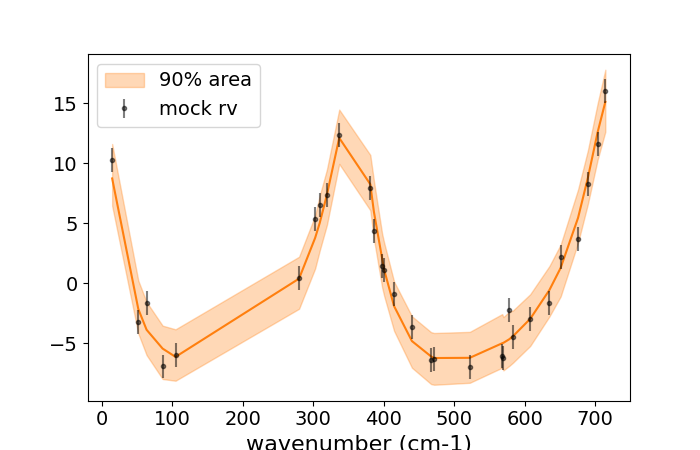
\includegraphics[width=\linewidth]{fig/rv_fit.png}
    \caption{視線速度データのフィット}
    \label{fig:rvfit}
\end{figure}
\section{ガウス過程$^\ddagger$}

$N$次元ガウシアン分布を
\begin{align}
    \Ng(\xv;\muv, \Sigma) \equiv \dfrac{1}{\sqrt{(2 \pi)^{N} |\Sigma|}} e^{- (\xv - \muv)^\top \Sigma^{-1}(\xv - \muv) /2  }
\end{align}
と表記する。また誤解がない場合、変数$\xv$を略して、
\begin{align}
    \Ng(\muv, \Sigma) \equiv \dfrac{1}{\sqrt{(2 \pi)^{N} |\Sigma|}} e^{- (\xv - \muv)^\top \Sigma^{-1}(\xv - \muv) /2  }
\end{align}
のように表記する場合もある。

\subsection*{相関ノイズとしてのガウス過程}
ガウス過程は、多変数正規分布
\begin{align}
\dv \sim \Ng(\zerov,\Sigma)
\end{align}
に従う確率変数$\xv$の確率過程のことである。いま$d_i$は時系列だとして、この多変数正規分布の共分散行列の各成分が、
\begin{align}
\Sigma_{ij} = K_{ij}(a, \tau) = a k(|t_i-t_j|; \tau)
\end{align}
のように、$t_i$と$t_j$の差の絶対値の関数として与えられれば、相関長$\tau$のガウス過程が得られる。
カーネル関数$k(t,\tau)$としてはいろいろなタイプがありうるが、例えばRBFカーネル
\begin{align}
 k_\mathrm{RBF}(t;\tau) = \exp{\left(- \frac{t^2}{2 \tau^2} \right)},
\end{align}
とMat\'{e}rn 3/2カーネル
\begin{align}
\label{eq:MaternA}
 k_\mathrm{M3/2}(t;\tau) = \left( 1 + \frac{\sqrt{3} t}{\tau} \right) e^{- \sqrt{3} t/\tau}. 
\end{align}
などがある。

このガウス過程にしたがったデータ点をサンプリングしてみると図\ref{fig:gp1}のようになる。ただしデータにさらに平均ゼロ、標準偏差$\sigma$のガウスノイズを足している。このノイズを便宜的に観測ノイズと呼んでおこう。
\begin{figure}[htb]
\begin{center}
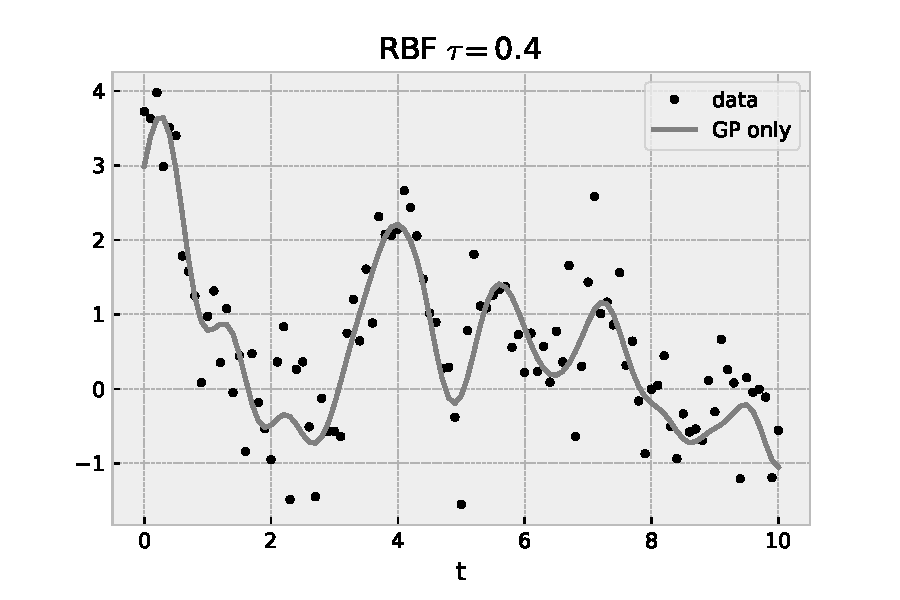
\includegraphics[width=\linewidth]{fig/gp/gp1.pdf}
\caption{ガウス過程からサンプルされたデータ。実線は$\sigma$の観測ノイズなし。\label{fig:gp1}}
\end{center}
\end{figure}



さてこのデータを元に$\tau$、$a$、$\sigma$をMCMCサンプリングしてみよう。平均ゼロ、標準偏差$\sigma$のガウスノイズの観測ノイズを足したということは確率モデルとしては、
\begin{eqnarray}
\label{eq:gpmodel0}
\dv &\sim& \Ng(\zerov,\Sigma^\prime ) \\
\Sigma^\prime &=& K(a, \tau) + \sigma^2 I
\end{eqnarray}
となる。この$\Sigma^\prime$はRBFカーネルを仮定し、さらに独立誤差を表す対角項を加える。つまり
\begin{align}
 \Sigma_{ij} (a, \tau, sigma) = a k_\mathrm{RBF} (|t_i - t_j|; \tau) + \sigma^2 I
\end{align}
となり、共分散はパラメタ$(a, \tau, \sigma)$を持つ。Exponential分布$E(x)$を用いて事前分布を構成すると、たとえば事前分布は
\begin{align}
    p(a) &= E(1) \\
    p(\tau) &= E(1) \\
    p(\sigma) &= E(1) 
\end{align}
となり、尤度は
\begin{align}
    p(\dv|a, \tau, \sigma) = \Ng(\zerov,  \Sigma (a, \tau, \sigma) )
\end{align}
のようにかける。つまりこれでMCMCを回すことができる。


HMCでサンプルした事後分布を可視化したものが図\ref{fig:gp2}である。
\begin{figure}[htb]
\begin{center}
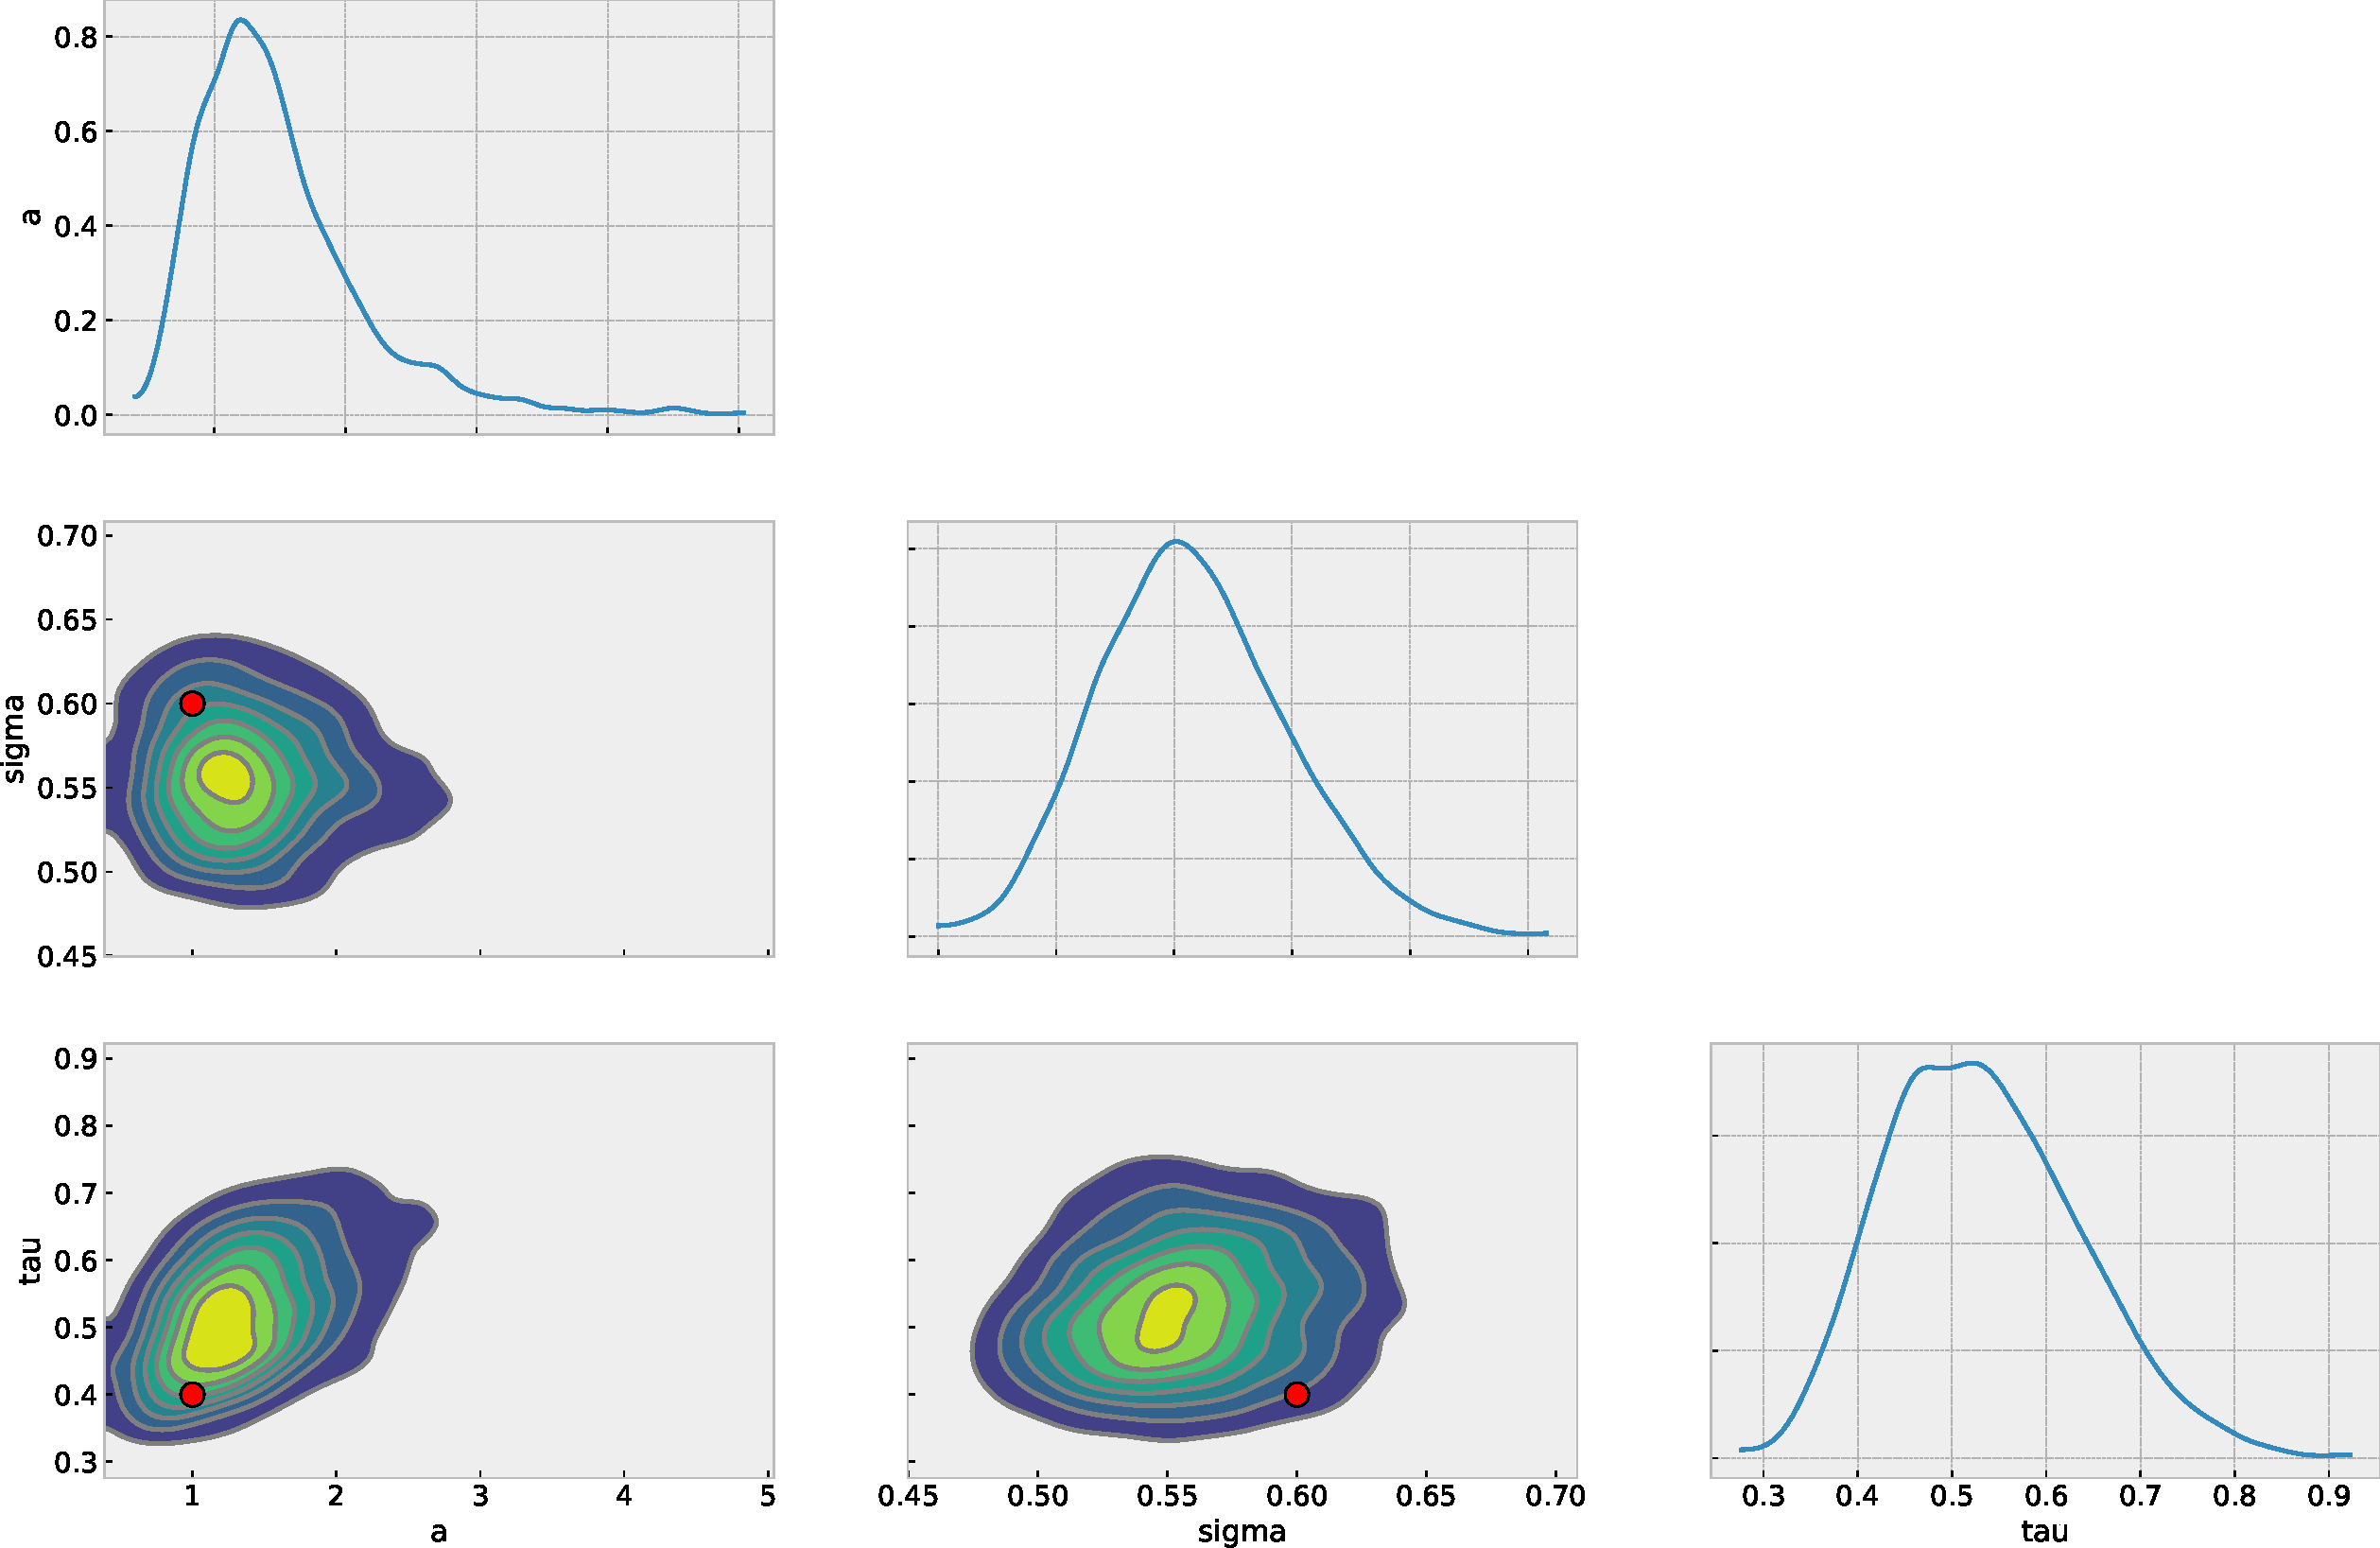
\includegraphics[width=\linewidth]{fig/gp/gp2.pdf}
\caption{\label{fig:gp2}}
\end{center}
\end{figure}
ところで、式(\ref{eq:gpmodel0})という観点のモデル化では、$\xv=\zerov$がモデル平均である。credible intervalを計算したものが図\ref{fig:gp3}となっているが、このことが直感的にわかる。
\begin{figure}[htb]
\begin{center}
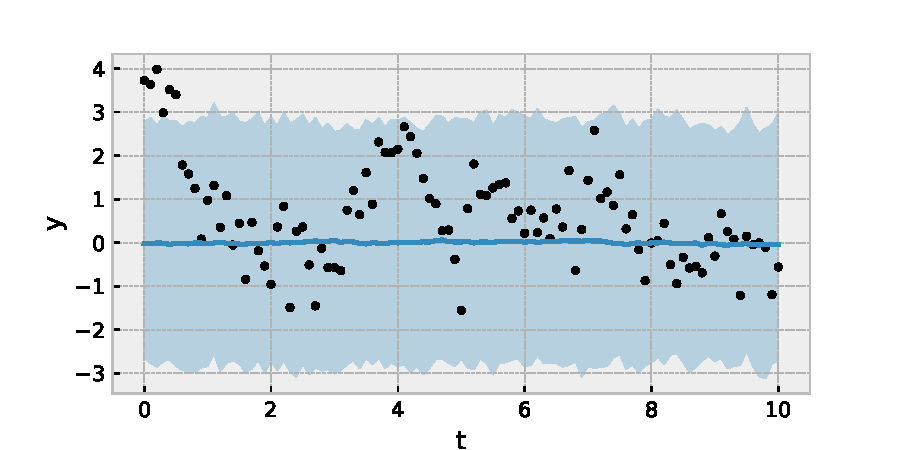
\includegraphics[width=\linewidth]{fig/gp/gp3.pdf}
\caption{\label{fig:gp3}}
\end{center}
\end{figure}


\subsection*{モデルとしてのガウス過程}

上記のガウス過程による解析は、モデルパラメタ$\mv$の事前分布(プライア)として
\begin{align}
p(\mv) = \Ng (\zerov,\Sigma)
\end{align}
と置き、
\begin{align}
d_i &= m_i + \epsilon \\
\epsilon &\sim \Ng (0,\sigma^2)
\end{align}
と見ることもできる。ここに$\epsilon$は観測ノイズに対応している。もう少しまどろっこしく書くとモデル$\gv$を恒等変換として、
\begin{align}
\label{eq:identif}
\gv(\mv) &= \mv \\
\dv &= \gv(\mv) + \epsilonv \\
\epsilonv &\sim \Ng (\boldsymbol{0} ,\sigma^2 I)
\end{align}
のように書ける。この場合、尤度関数が
\begin{align}
p(\dv|\mv) &= \Ng (\dv;\gv(\mv),\sigma^2 I) = \Ng (\dv;\mv,\sigma^2 I)
\end{align}
となる。そして、さらにこの事前分布の中にパラメタがあるという構造となっている。つまり
\begin{align}
\Sigma_{ij} = a k(|t_i-t_j|;\tau) 
\end{align}
としていて、このパラメタ$a$,$\tau$をハイパーパラメタという。そしてハイパーパラメタの事前分布(超事前分布またはハイパープライア)をさらに仮定するということに相当する。



ハイパーパラメタを固定した状態では、$\mv$の事後分布を解析的に書けることが知られている。ここでガウス過程の計算法を紹介しよう。まず多変数正規分布に多変数正規分布をかけても多変数正規分布である。そこで計算しなくてはならないのはexpのべきの部分のみである。多変数正規分布の「べき」部分は
\begin{align}
\label{eq:gp}
&- 2 \log{ \Ng(\mv;\muv, \Sigma) } = (\mv - \muv)^\top \Sigma^{-1} (\mv - \muv) \nonumber \\
&= \mv^\top \Sigma^{-1} \mv - 2 \mv^T \Sigma^{-1} \muv + \mathrm{const}. 
\end{align}
となっていることに注意すると、もしある多変数正規分布に従うことがわかっている確率密度分布$p(\mv)$が
\begin{align}
\label{eq:gpqu}
- 2 \log{ p(\mv) } = \mv^\top P \mv - 2 \mv^\top \qv + \mathrm{const},
\end{align}
のように書けたとすると、式(\ref{eq:gp})と比べることで、この確率密度分布は
\begin{align}
\label{eq:gpqusol}
p(\mv) = \Ng(\mv; P^{-1} \qv ,P^{-1}).
\end{align}
であることがわかる。

さて、いま事後分布は
\begin{align}
\label{eq:gppos}
p(\mv|\dv) \propto p(\dv|\mv) p(\mv) = \Ng (\dv;\mv,\sigma^2 I) \Ng (\mv;\zerov,\Sigma)
\end{align}
であるので、この「べき」部分を$\mv$について展開することで、
\begin{align}
\label{eq:gpposs}
&- 2 \log{[\Ng (\dv;\mv,\sigma^2 I) \Ng (\mv;\zerov,\Sigma)]} \nonumber \\
&= \mv^\top (\Sigma^{-1} + \sigma^{-2} I ) \mv - 2 \sigma^{-2} \mv^\top \dv + \mathrm{const.} 
\end{align}
と書けること、また
\begin{align}
\label{eq:gppossxx}
(\Sigma^{-1} + \sigma^{-2} I )^{-1} = \Sigma (I + \sigma^{-2} \Sigma )^{-1}
\end{align}
より
\begin{align}
\label{eq:gpposss}
p(\mv|\dv) = \Ng (\mv;\Sigma (\sigma^{2} I + \Sigma )^{-1} \dv, \Sigma (I + \sigma^{-2} \Sigma )^{-1} )
\end{align}
であることがわかった。

MCMCにより$\tau$と$\sigma$のサンプリングをすることができるが、これらのパラメタの事後分布は何を意味するか考えよう。これらは今の枠組みではハイパーパラメタとみなせるので、まとめて$\thetav = (a, \tau, \sigma)^\top$をハイパーパラメタとおく。ここからは$\thetav$も確率に入れて考えることにする。さて、今、$\mv$について周辺化した尤度
\begin{align}
\label{eq:gppozz}
p(\dv|\thetav) = \frac{p(\dv|\mv,\thetav) p(\mv,\thetav)}{p(\mv|\dv,\thetav)}
\end{align}
はやはり多変数正規分布となるが、また「べき」部分の$\dv$に関する部分だけ考えることにより
\begin{align}
\label{eq:gppozzp}
&- 2 \log p(\dv|\thetav) = \nonumber \\
&- 2 \log p(\dv|\mv,\thetav) + 2 \log p(\mv|\dv,\thetav) + \mathrm{const} \nonumber \\
&= - 2 \log \Ng(\dv|\mv, \sigma^2 I )  \nonumber \\
&+ 2 \log \Ng(\mv|\Sigma (\sigma^{2} I + \Sigma )^{-1} \dv, \Sigma (I + \sigma^{-2} \Sigma )^{-1} ) \nonumber \\
&= \dv^\top (\sigma^{2} I + \Sigma)^{-1} \dv + \mathrm{const.}
\end{align}
である。よって
\begin{align}
\label{eq:gmarg}
p(\dv|\thetav) =  \Ng (\dv; \zerov, \Sigma + \sigma^{2} I )
\end{align}
となる。
\underline{$\Sigma = K(\tau)$とすれば、式(\ref{eq:gpmodel0})と同じである。} 
すなわち、(超)事前分布として$p(\thetav)$を与えた時の周辺化事後分布
\begin{align}
\label{eq:gmpost}
p(\thetav|\dv) \propto p(\dv|\thetav) p(\thetav)
\end{align}
をサンプリングしていることになる。

図\ref{fig:gp2}はハイパーパラメタ$\tau$、$\sigma$の周辺化事後分布を示していることがわかった。つまり$k=0,..., N_s-1$に対して
\begin{align}
\label{eq:gmposts}
\thetav^\dagger_k \sim p(\thetav|\dv) \propto p(\dv|\thetav) p(\thetav)
\end{align}
をサンプリングしたことになる。さて、ではこのサンプルと式(\ref{eq:gpposss})を用いて、
\begin{align}
\label{eq:gpposssaq}
p(\mv, \thetav|\dv) = p(\mv|\thetav, \dv) p(\thetav|\dv)
\end{align}
であることから
\begin{align}
\label{eq:gpposssaahuq}
 p(\mv|\thetav^\dagger_k, \dv) &= \Ng ( \muv_k ,  K_k ) \\
 \label{eq:muvk}
 \muv_k &= K(a^\dagger_k,\tau^\dagger_k) ((\sigma^\dagger_k)^{2} I + K(a^\dagger_k,\tau^\dagger_k) )^{-1} \dv \\
  \label{eq:Kk}
 K_k &= K(a^\dagger_k,\tau^\dagger_k)(I + (\sigma^\dagger_k)^{-2} K(a^\dagger_k,\tau^\dagger_k) )^{-1} 
\end{align}
からサンプルした$\mv^\dagger_k$と$\thetav^\dagger_k$のセットは
\begin{align}
\label{eq:gpposssaqp}
(\mv^\dagger_k,\thetav^\dagger_k) \sim p(\mv, \thetav|\dv) 
\end{align}
とみなせることがわかる\footnote{ハイパーパラメタの点推定(いわゆるmaximum marginal likelihood=maximum evidence)を用いる方法については解説が多くあるが、周辺化事後分布から再サンプリングする議論についてはいまのところ文献が見つからない。ベイズ線形問題+ガウス過程の枠組みで以前、筆者が議論したことがあるので参考までに挙げておく\cite{2020ApJ...900...48K}。}。

HPDIを計算することで、図\ref{fig:gp4}の$\mv$のcredible intervalが求まる。ここで注意点としては、これはモデル$\mv$の90\% intervalであり、観測ノイズ部分を含んだ$\dv$の予測ではないという点である。
\begin{figure}[htb]
\begin{center}
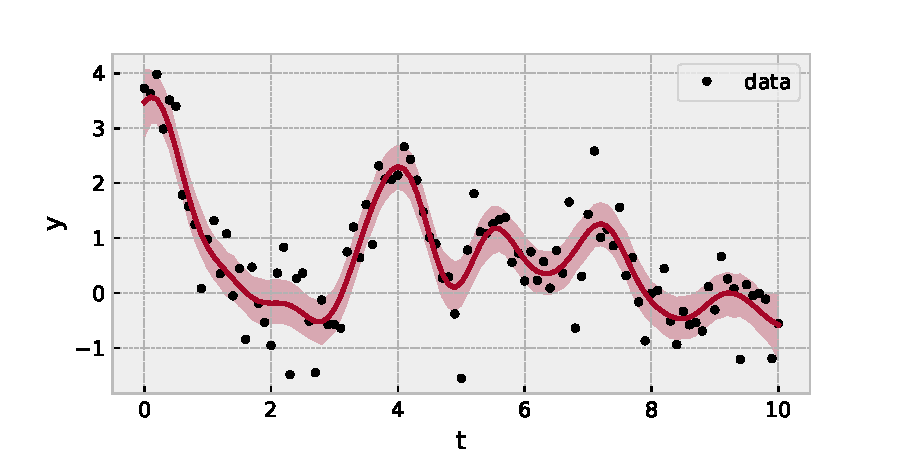
\includegraphics[width=\linewidth]{fig/gp/gp4.pdf}
\caption{\label{fig:gp4}}
\end{center}
\end{figure}

\subsection*{データ点にない位置の予測}

さて、一般に$t=t^\ast$での予測値はどうなるだろうか?以下では再度ハイパーパラメタを省略して表記する。まず、$\mv$、$\mva$がガウス過程に従うとき
\begin{align}
p(\mva|\mv) = \Ng (K_{\times}^\top K^{-1}  \mv, K_\ast - K_\times^\top K^{-1} K_\times)
\end{align}
である。ここに
\begin{align}
K_{ij} &= a k(|t_i-t_j|;\tau) \\
(K_{\times})_{ij} &= a k(|t_i-t^\ast_j|;\tau) \\
(K_{\ast})_{ij} &= a k(|t^\ast_i-t^\ast_j|;\tau) 
\end{align}

同様に
\begin{align}
\label{eq:predgp1}
p(\mva|\dv) =  \Ng (K_{\times}^\top K_\sigma^{-1}  \dv, K_{\ast} - K_\times^\top K_\sigma^{-1} K_\times)
\end{align}
となる。ここに
\begin{align}
(K_{\sigma})_{ij} = a k(|t_i-t_j|;\tau) + \sigma^2 \delta_{i,j}
\end{align}
($\delta_{i,j}$はクロネッカーデルタ)。ここで$p(\mva|\dv)$はあくまでモデルパラメタとしてのガウス過程の事後分布なので、観測ノイズの分は考慮されていない。

もし観測ノイズを含んだ予測を行いたいのならば、
\begin{align}
\dv^\ast = \mv^\ast + \epsilonv
\end{align}
というモデルに基づき、
\begin{align}
\label{eq:predgp2}
p(\dv^\ast|\dv) =  \Ng (K_{\times}^\top K_\sigma^{-1} \dv, K_{\ast,\sigma} - K_\times^\top K_\sigma^{-1} K_\times)
\end{align}
となるだろう。ここに
\begin{align}
(K_{\ast,\sigma})_{ij} &= a k(|t^\ast_i-t^\ast_j|;\tau) + \sigma^2 \delta_{i,j}
\end{align}
である。

というわけで、ハイパーパラメタ込みのサンプリングで式(\ref{eq:predgp1},\ref{eq:predgp2})のサンプリングを行いCredible Intervalを求める。同様にHPDIを求めたものが図\ref{fig:gp6}である。濃い色が$\mva$の、薄い色が$\dv^\ast$のcredible intervalである。

\begin{figure}[htb]
\begin{center}
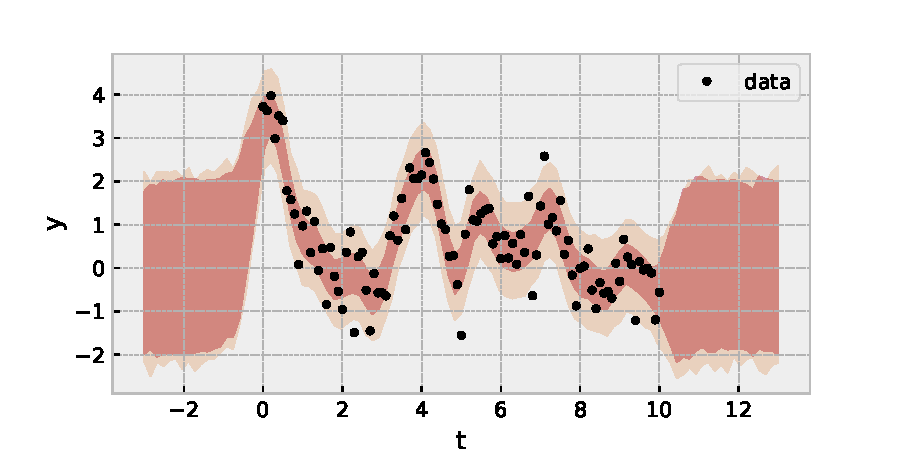
\includegraphics[width=\linewidth]{fig/gp/gp6.pdf}
\caption{\label{fig:gp6}}
\end{center}
\end{figure}

\subsection*{解析モデルにガウス過程モデルを加える$^\ddagger$}

さて、ここまではモデルとしては平均値がゼロのガウス過程により生成されるモデル
\begin{align}
\mv \sim \Ng ({\bf 0},\Sigma(\tv)) 
\end{align}
を考えていた。ここでは一般に平均値が$t$の関数となるガウス過程によりデータが生成される場合を考えよう。すなわち
\begin{align}
\label{eq:modelgp}
\mv \sim \Ng (\fv(\tv),\Sigma(\tv)) 
\end{align}
の場合を考えよう。ここに$\fv(\tv)$は$f(t)$に対し、$\tv=(t_0,t_1,\cdots t_{N-1})$を要素ごとに適用したベクトル版である。ここでは$f(t)$として
\begin{align}
f(t) = k e^{-(t-T_0)^2/2 s^2} \sin{(2 \pi t/P)}
\end{align}
というものを考えてみよう。上では簡単に$f(t)$と書いたが、パラメタを$\thetav=(T_0,k,s,P)$として$f(t;\thetav)$という表記も併用する。

式(\ref{eq:modelgp})の共分散行列をRBFカーネルとして選択すると、例えば、図\ref{fig:gp1m}上のようなデータが生成される。ここで$\tau=3$であり$f(t)$より比較的ゆったりとしたトレンドが乗っているのが見て取れるだろう。
\begin{figure}[htb]
\begin{center}
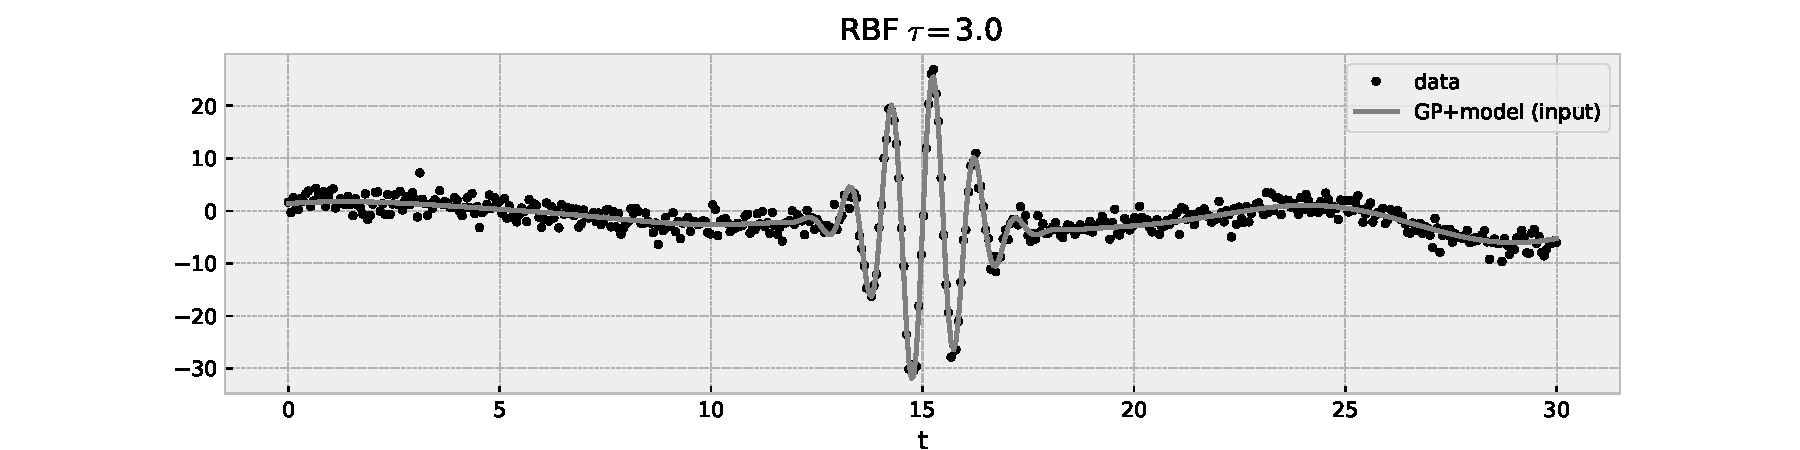
\includegraphics[width=\linewidth]{fig/gpmodel/gp1.pdf}
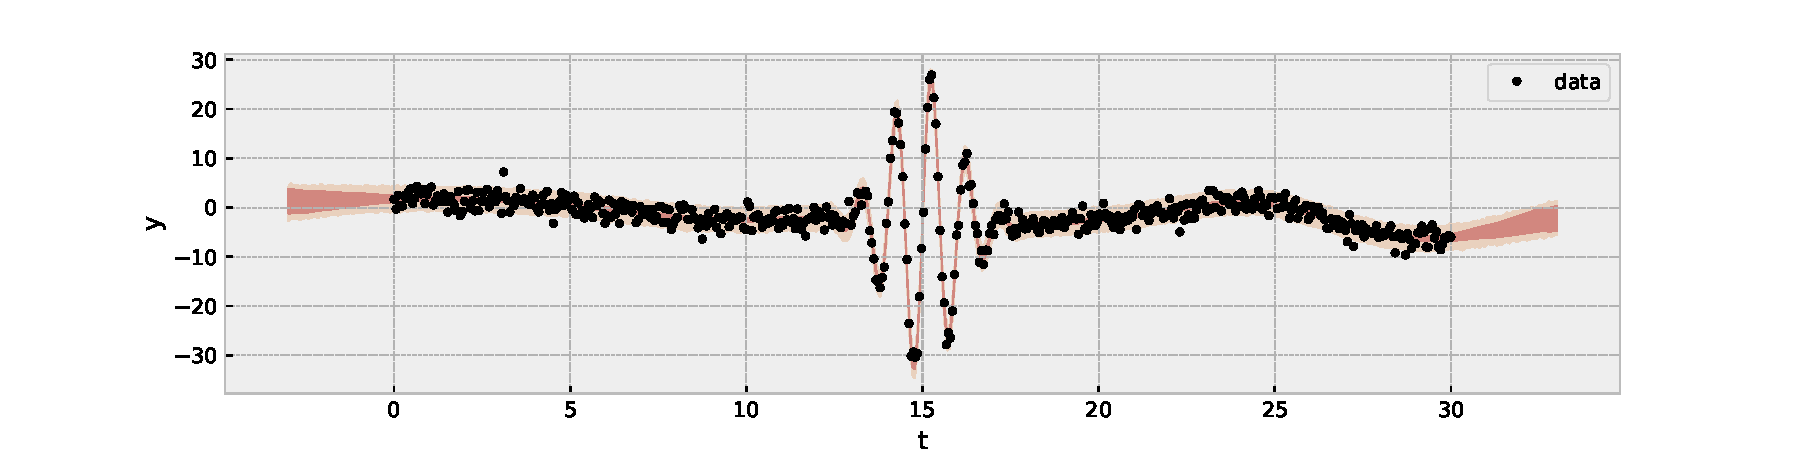
\includegraphics[width=\linewidth]{fig/gpmodel/gp6.pdf}
\caption{実線は$\sigma$の観測ノイズなし。\label{fig:gp1m}}
\end{center}
\end{figure}
このようなモデルをHMCフィットするというのは、シグナル$f(t)$と相関のあるノイズ+観測ノイズをモデル化し、$f(t)$の持つパラメタを推定したいときに対応する。


$\fv(\tv)$がわかっている場合、観測ノイズを含まない、および、含んだ予測は、それぞれ、
\begin{align}
\label{eq:predgp_model}
&p(\mva|\dv) =   \nonumber \\
&\Ng (\fv(\tv^\ast) + K_{\times}^\top K_\sigma^{-1}  (\dv - \fv(\tv)),  K_{\ast} - K_\times^\top K_\sigma^{-1} K_\times) \\
&p(\dv^\ast|\dv) =   \nonumber \\
&\Ng (\fv(\tv^\ast) + K_{\times}^\top K_\sigma^{-1} (\dv - \fv(\tv)), K_{\ast,\sigma} - K_\times^\top K_\sigma^{-1} K_\times)
\end{align}
となる。$\fv(t)$の持つパラメタ$\thetav=(T_0,k,s,P)$はHMCでサンプリングされるから、例えば後者なら、サンプリングされた各$\thetav^\dagger_k$をもちいて
\begin{align}
\label{eq:predgp2_}
&\dv^\ast_k \sim  \Ng (\mu_k, K_k) \\
&\mu_k = \fv(\tv^\ast; \thetav^\dagger_k) + K_{\times}^\top K_\sigma^{-1} (\dv - \fv(\tv; \thetav^\dagger_k)) \\
&K_k = K_{\ast,\sigma} - K_\times^\top K_\sigma^{-1} K_\times
\end{align}
をサンプリングすれば、予測のサンプリングができる。というわけで、以下のようにモデル$f(t)$込みのGPのフィットを行うことができる(図\ref{fig:gp1m}下)。



\chapter{系外惑星からのスペクトル}



本章では惑星自身のもつ情報が埋め込まれたシグナルの概観を行う。惑星シグナルは、大まかに分けると恒星光が惑星大気を透過したもの、惑星からの熱輻射、もしくは恒星光が惑星により反射されたもののいずれかの形態をとる(表\ref{tab:spec_sep})。これらの惑星シグナルを分光することで系外惑星の大気を調べることができる。いずれの場合も、系外惑星大気を通過する光が、大気中の分子・原子や雲といった成分によって波長方向に吸収や散乱といった影響を受けて変化する。その変化をスペクトルを通じて検出することで大気を理解するということである。通過する光は上の三つの形態に応じて惑星自身が放つ輻射光と恒星光の光を利用する方法に分けることができる。前者は惑星からの輻射光という意味で今後「輻射光」と略記する。後者はそれぞれトランジット透過光と反射光であり、この二者は恒星光に惑星シグナルが刻まれるという意味でパッシブな手法であるとも見ることができる。

\begin{table}[htbp]
\footnotesize
  \centering
  \caption{スペクトル種類の分類}
  \label{tab:spec_sep}
  \begin{tabular}{ccc}
    \hline
    スペクトル & 手法 & 現在の主な対象 \\
    \hline
    透過光 & 透過光分光 & トランジット系\\
                & 高分散分光 & トランジット系\\
    \hline
    輻射 & 二次食分光 & トランジット系\\
                & 直接撮像 & 若い惑星\\
                & 高分散分光 & 明るい系 \\
    \hline
    反射 & 直接撮像 & 地球近傍 \\ 
                & 高分散分光 & 明るい系 \\
  \end{tabular}
\end{table}




系外惑星分光の最大の問題は、いかに恒星光の影響を分離・除去し、惑星光のスペクトルを取り出すかというところにある。表\ref{tab:light_sep}に、分離方法に基づいた手法の分類を示す。まずデータ解析で分離すると手法は、恒星光と惑星光がまったく分離されていないスペクトルを取得し、データ解析的に惑星光を分離する手法である。トランジット系では、トランジット時の減光から、惑星の半径が計測できるが、これを波長ごとに行い、大気情報を得ることができる。この手法は\underline{透過光分光}と呼ばれる。トランジット系では、惑星が恒星の背面に隠れる時に、惑星光が隠された分やはり減光する。これは\underline{二次食}と呼ばれ、惑星光の分離に用いることができる。この二つの手法はトランジット系のみに用いることができる方法である。次に恒星光と惑星光が混ざったものに対し\underline{高分散分光}を利用し惑星光を取り出す手法がある。この手法では恒星と惑星の視線速度差を利用して、惑星由来の成分、具体的には、惑星大気の分子や原子の吸収線を同定する。この手法は非トランジット系にも適用可能である。最後に、装置的に恒星光を除去する手法が\underline{直接撮像法}である。この手法は、主に恒星光と惑星光の光の強度比(コントラスト)と恒星と惑星の分離角によって検出できるかどうかが決まる。分離角は観測者に近いほど相対的に大きくなるので、地球近傍の惑星系がターゲットとなる。また現在の直接撮像の性能では、コントラストが穏やかなものしか検出できないため、惑星が高温で自ら光っている若い惑星系のみが検出されている。ただし、今後の宇宙直接撮像や地上の装置性能の向上に伴い、原理的には通常の惑星系でも検出可能である。


\begin{table}[htbp]
\footnotesize
  \centering
  \caption{系外惑星分光法の分類}
  \label{tab:light_sep}
  \begin{tabular}{ccc}
    \hline
    分離手段 & 手法 & 対称 \\
    \hline
    データ解析 & 透過光分光 & トランジット惑星 \\
     & 二次食分光 & トランジット惑星 \\
     & 高分散分光 & トランジット or 高温惑星 \\
    \hline
    装置 & 直接撮像 & 若い惑星 or 地球近傍\\
    \hline
  \end{tabular}
\end{table}



\section{トランジット現象 \label{ss:transit}}

\begin{figure}[]
 \begin{center}
	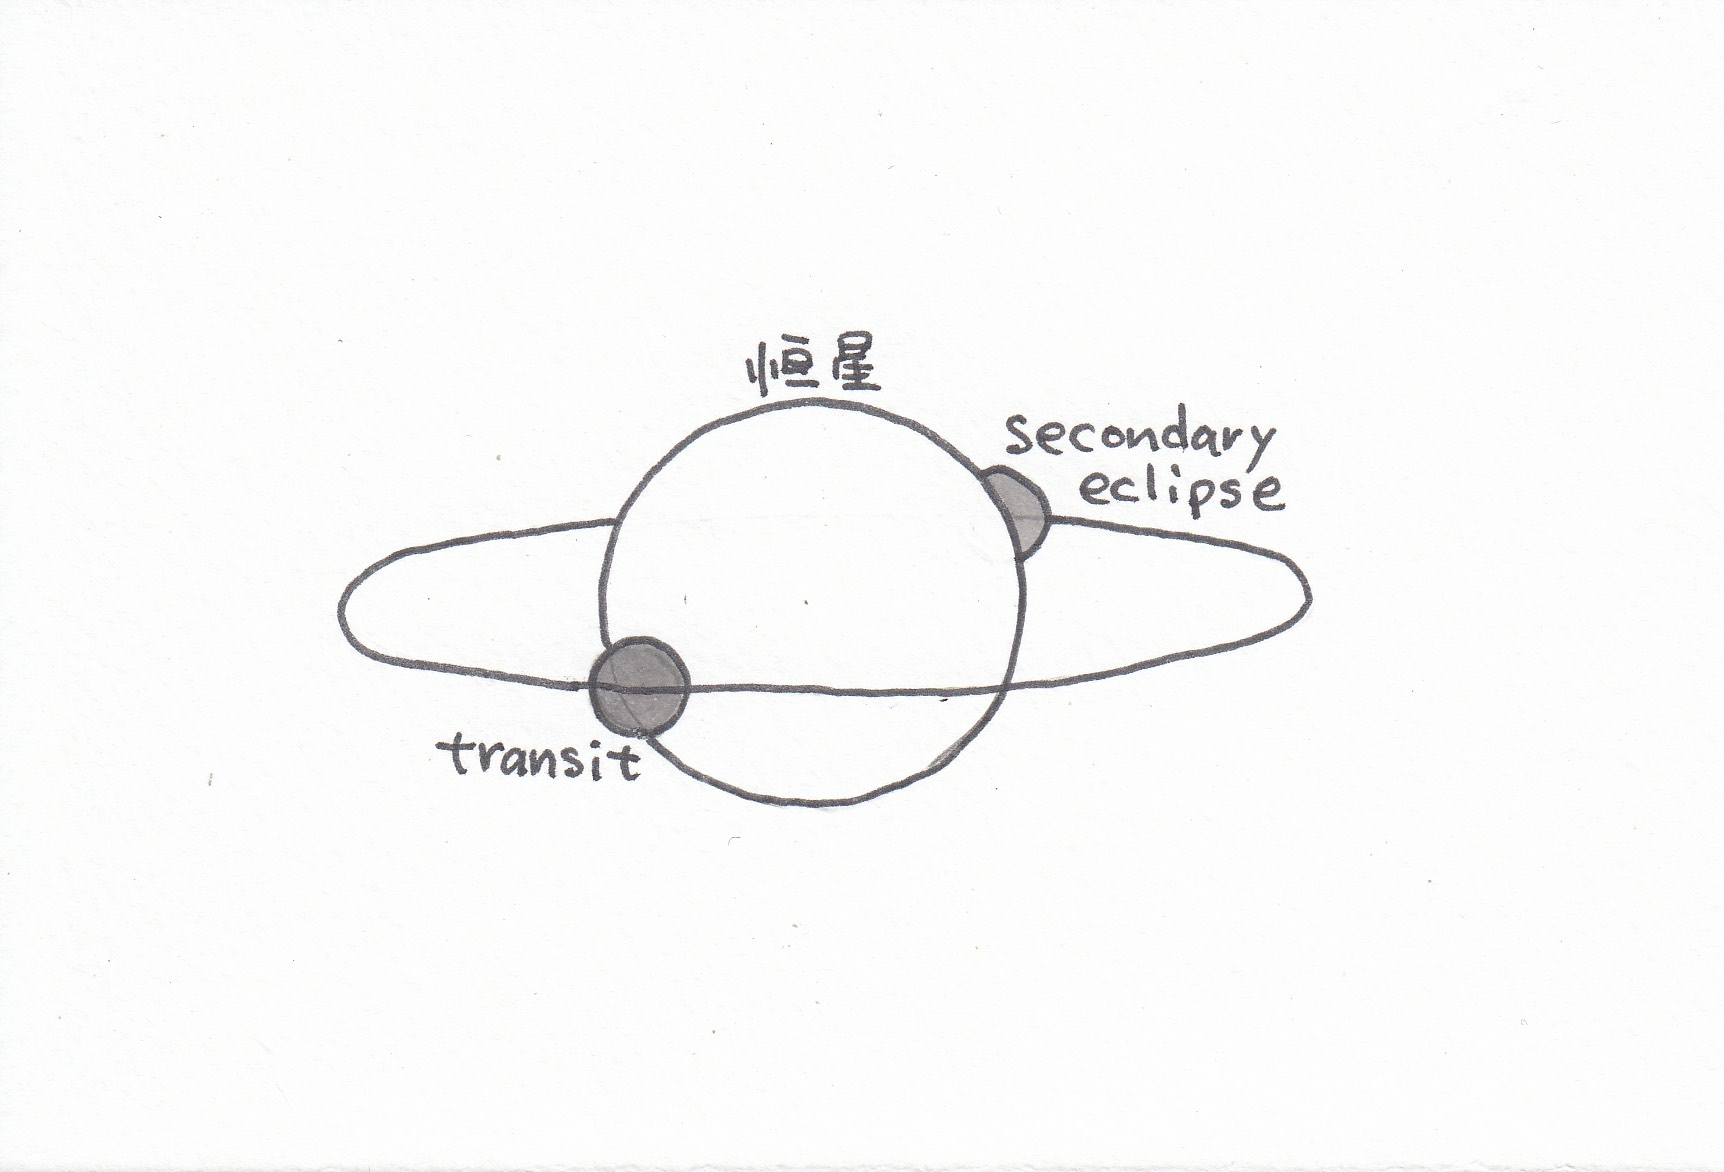
\includegraphics[width=\linewidth]{fig/transit.jpg}
	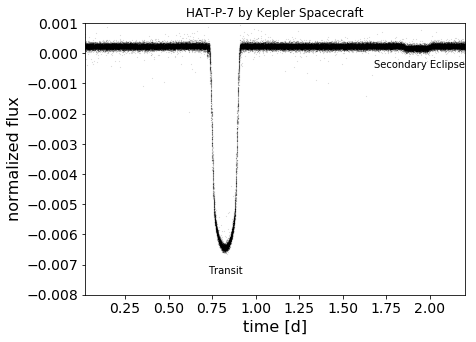
\includegraphics[width=\linewidth]{fig/Hatp7.png}
 \end{center}
 \caption{トランジット系の概念図(上)とホットジュピターHAT-P-7bによるトランジット減光曲線の例(下)。\label{fig:hatp7b}}
\end{figure} 

主星フラックスの変動にも惑星によるシグナルが含まれる。最も分かりやすいのは主星の前面を惑星が通過する時にできる陰によるフラックス減少である{\bf トランジット減光}\index{とらんじっとげんこう@トランジット減光}である(図\ref{fig:hatp7b})。トランジット系は逆に惑星が主星の後ろに隠れることによる減光も観測されている。後者は二次食\index{にじしょく@二次食}(secondary eclipse)\index{secondary eclipse@secondary eclipse}とか単にocclutation\index{occlutation@occlutation}と呼ばれている。

惑星がトランジットする確率は、円軌道かつ$R_p \ll R_\star$を仮定すると、図\ref{fig:transitprob}で示された領域であるから
\begin{align}
p_\mathrm{tra} = \sin{(R_\star/a)} \sim \frac{R_\star}{a} = 0.005 \left(\frac{R_\star}{R_\odot}\right) \left(\frac{a}{1 \mathrm{\, au}}\right)^{-1}
\label{eq:tranp}
\end{align}
となり、G型星まわりのハビタブル惑星だと0.5 \%である。


\begin{figure}[!hbt]
 \begin{center}
	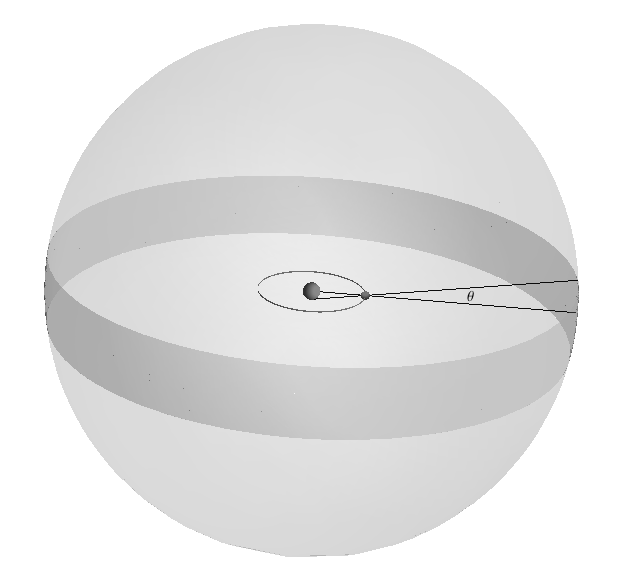
\includegraphics[width=\linewidth]{fig/transit_prob_bw.png}
\end{center}
	\caption{トランジットして見える立体角方向(帯部分)。中に恒星と惑星軌道が描かれている。外側の球の半径は、観測者から惑星系までの距離$d$であるので、$a \ll d$と見なせる。するとランダムな視線方向で帯領域をとる確率は$4 \pi \sin{\theta}/ (4 \pi) \approx R_\star/a$となる。\label{fig:transitprob}}
\end{figure} 

\subsection*{トランジットライトカーブ}

\begin{figure}[htb]
\begin{center}
	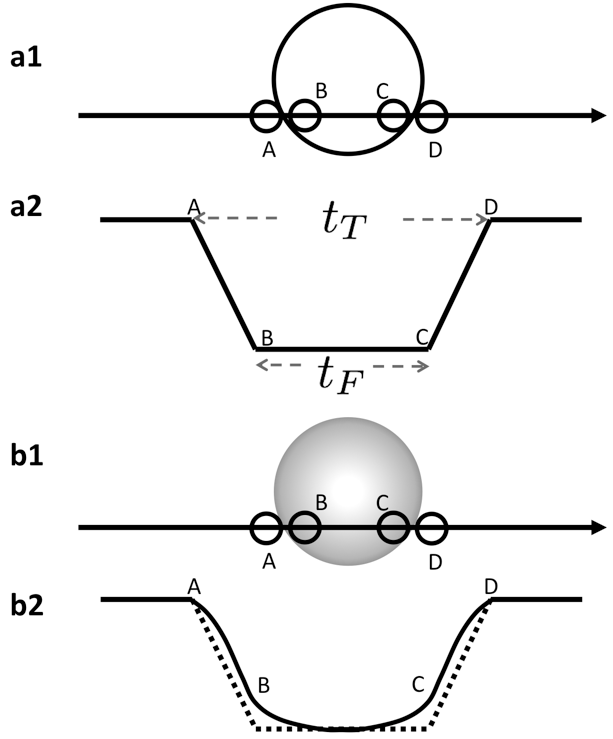
\includegraphics[width=\linewidth]{fig/transitmodel.png}
	\caption{トランジットライトカーブの幾何。aは恒星が一様に光っている場合のライトカーブ。実際は恒星は淵側が暗い(周辺減光)ためにbのようなライトカーブとなる。}
	\label{fig:transitmodel}
\end{center}
\end{figure} 

さてトランジットのライトカーブから、系外惑星系のどういった物理量が分かるのだろうか?まず複数回のトランジットが観測されれば、
\begin{itemize}
\item 公転周期$P$
\end{itemize}
を知ることができる。また、トランジット深さは、
\begin{itemize}
\item 惑星半径と恒星半径の比$k \equiv R_p/R_\star$
\end{itemize}
の二乗となるので、この$k$を知ることができる。トランジットの継続時間から
\begin{itemize}
\item 惑星の通過時間(duration) $T_\mathrm{tot}$
\end{itemize}
を知ることができる。さらに細かく見ると、もし恒星が一様に光っているという近似の元では、図\ref{fig:transitmodel}aに示されるように、ingress・egress時もわかる。つまり惑星が恒星に入るとき出る時に、惑星が恒星に入り始めてから、完全に出るまでの時間$t_T$と、惑星が完全に恒星の全面に入っている期間、$t_F$が測定できるというように言い換えることもできよう。恒星は、実際は周辺減光(Limb darkening)をしており、実際のライトカーブは図\ref{fig:transitmodel}bのようになる。そこで通常、周辺減光のモデル化を行うことで$t_T$と$t_F$も求めることができる。周辺減光のモデルとしては以下のquadratic limb-darkening law
\begin{align}
I(\mu) = I(\mu=1) [ 1 - u_1 (1 - \mu) - u_2 (1 -\mu)^2] 
\end{align}
がよく用いられる。ここに$\mu = \cos{\psi}$であり$\psi$は光球面の法線ベクトルと視線ベクトルのなす角度である。つまり中心で$\mu=1$、ディスク境界で$\mu=0$となる。上記モデルは円盤で積分すると$\pi R_\star^2 (1 - u_1/3 - u_2/6) I(\mu=1)$になることに注意。今、$k$がわかっているので、$t_T$, $t_F$から幾何学的に
\begin{itemize}
\item 衝突径数(impact parameter): $b = \frac{a}{R_\star} \cos{i} $
\end{itemize}
も知ることができる。恒星スペクトルのモデルや後述する恒星密度$\rho_\star$の情報を用いて$R_\star$と$M_\star$が推定できれば、周期$P$がわかっているとケプラー第3法則から$a$を推定することができる。これにより軌道傾斜角$i$を決定することができる。もし視線速度の測定されているトランジット系が存在すれば、軌道傾斜角$i$がわかっているので惑星質量$M_p$が求まるので、惑星の平均密度
\begin{align}
\rho_p \equiv \frac{3 M_p}{4 \pi R_p^3}
\end{align}
が推定できるということである。これにより系外惑星の大まかな分類が可能になった。

円軌道の場合、通過時間は$T_\mathrm{tot} = 2 \sqrt{1-b^2} R_\star/v$である。ここに$v$は惑星の通過速度である。
惑星の質量を無視したケプラー第三法則
\begin{align}
 P^2 = \frac{4 \pi^2}{G M_\star} a^3 
\end{align}
を$v=2 \pi a/P$であることに注意して変形すると
\begin{align}
v^3=2 \pi G M_\star/P 
\end{align}
となるので、$T_\mathrm{tot}^3 \propto  P/\rho_\star $となり、周期・衝突径数がわかっていると、通過時間からは恒星密度$\rho_\star$がわかることになる。逆にだいたいの通過時間を知っておくため $b=0$のときを書いてみよう。この場合、
\begin{align}
T_\mathrm{tot}  &= \left( \frac{3  P}{\pi^2 G \rho_\star} \right)^{1/3} \\
&= 2.6 \mathrm{h} \left(\frac{P}{3 \mathrm{day}}\right)^{1/3} \left(\frac{\rho_\star}{\rho_\odot}\right)^{-1/3} \\
&= 30  \mathrm{h} \left(\frac{P}{12 \mathrm{yr}}\right)^{1/3} \left(\frac{\rho_\star}{\rho_\odot}\right)^{-1/3} 
\end{align}
となる。二行目はホット・ジュピターの典型値で三番目は木星の場合を仮定している。このように周期が数年以上になっていくと、通過時間が一日を超えるようになってくる。また、巨星の場合は、恒星密度が桁で小さくなるので通過時間がやはり長くなる。

\begin{itembox}{{\it column} -- 周期とライトカーブ形状 $\,^\dagger$}
%\tiny
\footnotesize
円軌道を仮定すると幾何的考察からから、
\begin{align}
\label{eq:totald}
\sin{ \left( \frac{\pi t_T}{P} \right)}  = \frac{R_*}{a} \sqrt{\frac{(1+k)^2 - b^2}{\sin^2{i}}}, \\
\label{eq:totalf}
\sin{ \left( \frac{\pi t_F}{P} \right)}  = \frac{R_*}{a} \sqrt{\frac{(1-k)^2 - b^2}{\sin^2{i}}},
\end{align}
が得られる。ここで、$\sin{(\pi t_T/P)} \sim \pi t_T/P$、$\sin{(\pi t_F/P)} \sim \pi t_F/P$と近似すれば、
\begin{align}
\label{eq:ra}
\frac{R_\star}{a} = \frac{\pi}{2 \sqrt{k}} \frac{\sqrt{t_T^2 - t_F^2}}{P} \sin{i}.
\end{align}
が得られる。さらに惑星の質量を無視したケプラー第三法則
\begin{align}
 P^2 = \frac{4 \pi^2}{G M_\star} a^3 
\end{align}
を用い$\sin{i} \sim 1$とすると、
\begin{align}
\label{eq:pk}
P &= \frac{\pi G}{32} \frac{M_\star}{R_\star^3} \left( \frac{t_T^2 -t_F^2}{k} \right)^{\frac{3}{2}} \\
 &= \frac{\pi^2 G}{24} \rho_\star \left( \frac{t_T^2 -t_F^2}{k} \right)^{\frac{3}{2}} 
\end{align}
が得られる。最後の式で未知の量は、恒星の平均密度$\rho_\star$だけであり、トランジットライトカーブ解析から恒星の平均密度という物理量が分かることが示される。
\end{itembox}

\section{透過光分光スペクトル}

透過光分光はトランジット深さを波長方向に展開して測定する。波長依存性を含めたトランジット深さは
\begin{align}
\delta (\lambda) = \left( \frac{R_p(\lambda)}{R_\star} \right)^2
\end{align}
のように表される。ここでは恒星半径の波長依存性は無視している。ここに$R_p(\lambda)$は、光が透過しなくなる大気の高さに対応する半径となる。この高さは大気中の原子・分子吸収や散乱もしくは固体表面で決まる。図\ref{fig:transmission}に固体表面を持つ惑星に吸収のある分子を持つ大気がある場合の透過光分光の例を示す。分子吸収のない波長では、固体表面が$R_p$となる一方、吸収がある波長では大気中の光学的深さが1になる付近が$R_p$となるため、トランジット深さが少し深くなる。この違いを捉えることで大気中の分子を検出できる。この例では、分子吸収以外の波長の連続成分が固体表面で決まるとしたが、他の場合として、連続吸収やレイリー散乱、雲による散乱、強い吸収線のウイング、弱い多数の吸収線の集合であるpseudo continuumなどもありうる。

\begin{figure}[htb]
\begin{center}
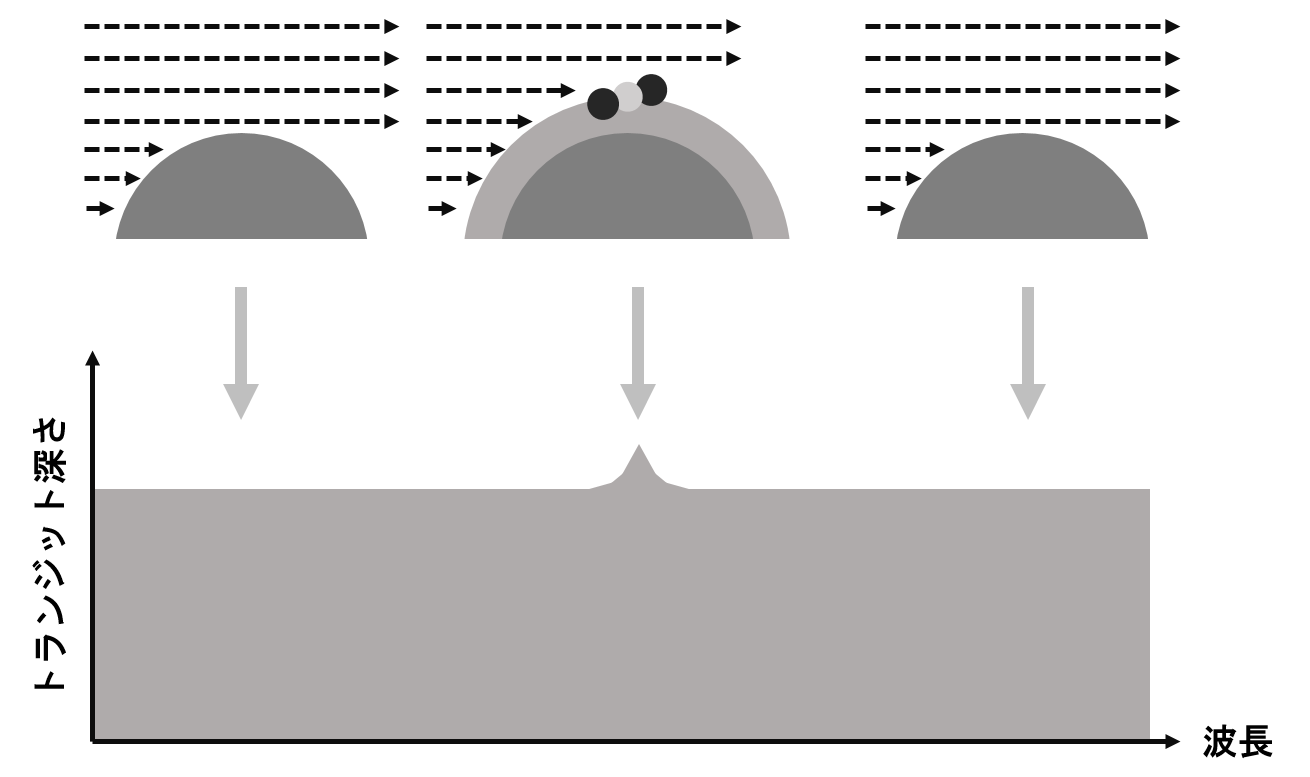
\includegraphics[width=\linewidth]{fig/transmission.png}
\caption{透過光分光の仕組み。\label{fig:transmission}}
\end{center}
\end{figure}


\section{惑星からの光}

恒星光が惑星にやってくると一部は吸収され熱となり、一部は熱化されることなく宇宙に返される。前者は熱化されたエネルギーが輻射光として宇宙に返される。惑星が形成されて間もないと、惑星内部からのエネルギーもこれに加わる。後者は、光子をそのまま返す過程であり、一般的には反射・散乱と呼ばれる。散乱は大気中で確率的に光が進行方向を変更するが、反射は地表や雲などで離散的に進行方向を変更する。

系外惑星からの光を考える時、惑星が球体であることを適切に考慮しないとならない。輻射光は球体全体からの強度を考えねばならないし、さらに反射光は恒星と惑星と観測者の相対的な位置関係に左右される。

%ここでは惑星内部からのルミノシティを$L_\mathrm{int}$とし、


\begin{figure}[h]
 \begin{center}
	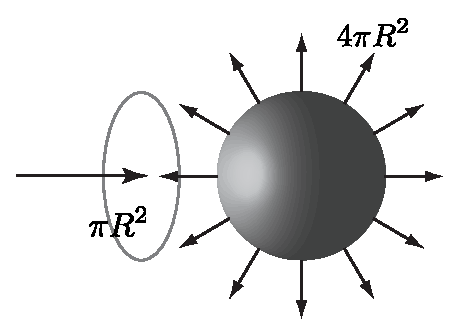
\includegraphics[width=\linewidth]{fig/io.eps}
\end{center}
	\caption{惑星へ入射してくる恒星光と惑星表面から出ていく輻射光。}
	\label{fig:io}
\end{figure} 

半径$R$の惑星が受け取るエネルギーは、恒星フラックス密度 \index{こうせいふらっくすみつど@恒星フラックス密度} (stellar flux density) $S$を用いて
\begin{align}
\label{eq:lab}
L_{\mathrm{ab}}=(1-A) \pi R^2 S  
\end{align}
と書くことができる。$\pi R^2$は惑星の断面積である(図\ref{fig:io}参照)。$A$は惑星全体の反射率(アルベド\index{アルベド@アルベド}という)で$(1-A)$の項は反射して宇宙に返された分を除いている。恒星光を黒体輻射と考えると、恒星フラックス密度は
\begin{align}
  \label{eq:starfluxdens}
S= \frac{L_\star}{4 \pi a^2} = \frac{4 \pi R_\star^2 \sigma T_\star^4}{4 \pi a^2}\,\,\mathrm{[W/m^2]} 
\end{align}
である。$a$は公転半径、$R_\star$は恒星半径、$T_\star$は恒星温度、$\sigma$はシュテファンボルツマン定数である。地球における$S_\odot =1370 \mathrm{W/m^2}$は太陽定数\index{たいようていすう@太陽定数}とよばれる。
一方、惑星からの放射を温度$T_{\mathrm{eq}}$の黒体輻射とすると放射エネルギーは
\begin{align}
\label{eq:lem}
L_{\mathrm{em}} = \beta ( 4 \pi R^2 \sigma T_{\mathrm{eq}}^4 ) + L_\mathrm{int}
\end{align}
とかける。ここで$ L_\mathrm{int}$は惑星自身のエネルギー放射である。若い惑星ではこの項が卓越しているため自己放射惑星と呼ばれる。

$\beta$は熱分配の度合いを表す係数で、瞬時に全球に一様に分配する極限$\beta=1$と、恒星光のあたっている半球だけに分配される場合$\beta=0.5$の間の値をとる。潮汐力により公転と自転が一致(潮汐ロック)しているような恒星に近い惑星では、地球に対する月のように、惑星の同じ面が常に恒星方向を向くために導入される補正である。


通常のmatureな惑星の場合、自己放射が無視できるため$L_\mathrm{int}=0$とおける。この場合、恒星からの吸収エネルギーが輻射エネルギーと釣り合うはずである。
\begin{align}
\label{eq:lemeqi}
  L_{\mathrm{em}} = L_{\mathrm{ab}}
\end{align}
とした時(放射平衡)の$T_{\mathrm{eq}}$を放射平衡温度\index{ほうしゃへいこうおんど@放射平衡温度}(単に平衡温度ともいう)と呼ぶ。この時、式(\ref{eq:lab})から式(\ref{eq:lemeqi})までを用いると
\begin{align}
  \label{eq:eqteq}
 \frac{T_{\mathrm{eq}}^4 a^2 }{T_\star^4 R_\star^2} = \frac{1-A}{4 \beta}
\end{align}
となる。つまり
\begin{align}
 T_\mathrm{eq} &= \left(\frac{1-A}{4 \beta}\right)^{\frac{1}{4}} T_\star \sqrt{\frac{R_\star}{a}} \\
&= 396 \mathrm{K}  \left(\frac{1-A}{4 \beta}\right)^{\frac{1}{4}} \left( \frac{T_\star}{5800 \mathrm{K}}\right) \left( \frac{R_\star}{R_\odot}\right)^{\frac{1}{2}} \left( \frac{a}{1 \mathrm{au}}\right)^{-\frac{1}{2}} \\
&= 396 \mathrm{K}  \left(\frac{1-A}{4 \beta}\right)^{\frac{1}{4}} \left( \frac{L_\star}{L_\odot}\right)^{\frac{1}{4}} \left( \frac{a}{1 \mathrm{au}}\right)^{-\frac{1}{2}}
\end{align}
となる。

ここで惑星表面が受け取る平均的な恒星フラックスを定義しておこう。式(\ref{eq:lab})より
\begin{align}
\label{eq:aveinpuF}
  F_\star &\equiv \frac{L_{\mathrm{ab}}}{4 \pi R^2}= \frac{(1 - A)}{4} S \\
  &= 240 \left(\frac{1-A}{0.7}\right) \left(\frac{S}{S_\odot}\right) \mathrm{W/m^2} 
\end{align}
のように$S$と結びつく。この式は、恒星の入射エネルギーから惑星の反射分を取り除き、図\ref{fig:io}に示すような断面円で入ってきた入射フラックスが自転により球面へ分配される効果を表す係数$1/4$をかけたものになるという描像を表している。惑星が受け取る平均フラックス密度と放射平衡温度には、
\begin{align}
  \label{eq:teq}
\sigma T^4_{\mathrm{eq}} = F_\star/\beta 
\end{align}
の関係にあることもわかる。

\subsection*{Radiance, Irradiance}

惑星や恒星は遠方から見れば点であり、近づいてみれば通常、連続的に密度が変わる三次元構造を持っている。しかし表面上のある基準球面、たとえば地球なら惑星表面や大気上端の高度一定面、恒星なら光球面などを考えると、ある面からの放射や、ある面への放射を考える事で、計算が易しくなる。そこで、まず、ある有限面積の表面からの放射や、表面への放射を定量化するための量を定義しよう。微小面積$d A$からある${\bf \Omega}$方向に$d \Omega$のコーン内(図\ref{fig:int}左)を通過する単位時間・単位波長あたりのエネルギー$d E$を考える。${\bf n}$は単位法線ベクトルである。$d E$自体は、見かけの投影面積$\cos{\theta} d A$に比例するので、
\begin{align}
d E = L_{\uparrow}(\theta,\phi) \cos{\theta} d A d \Omega d \nu
\end{align}
のように比例定数を、radiance (放射輝度) \index{Radiance@Radiance} $L_{\uparrow}$として定義すれば、投影の効果を除いて放射を定義できる。単位は例えば[$\mathrm{W/m^2/sr/\mu m}$]となる。$dA$から${\bf n}$方向に流れるネットのエネルギーをirradiance (放射照度) \index{Irradiance@Irradiance} $E_{\uparrow}$といい
\begin{align}
E_{\uparrow} &= \int_{\mathrm{us}} d E = \int  d \Omega L_{\uparrow} (\theta,\phi) \cos{\theta} \\
\label{eq:rad}
&= \int_{0}^{2 \pi} d \phi  \int_{0}^{\pi/2} d \theta L_{\uparrow} (\theta,\phi) \cos{\theta} \sin{\theta}
\end{align}
となる。usは上半球面の意味である。

\begin{figure}[]
 \begin{center}
	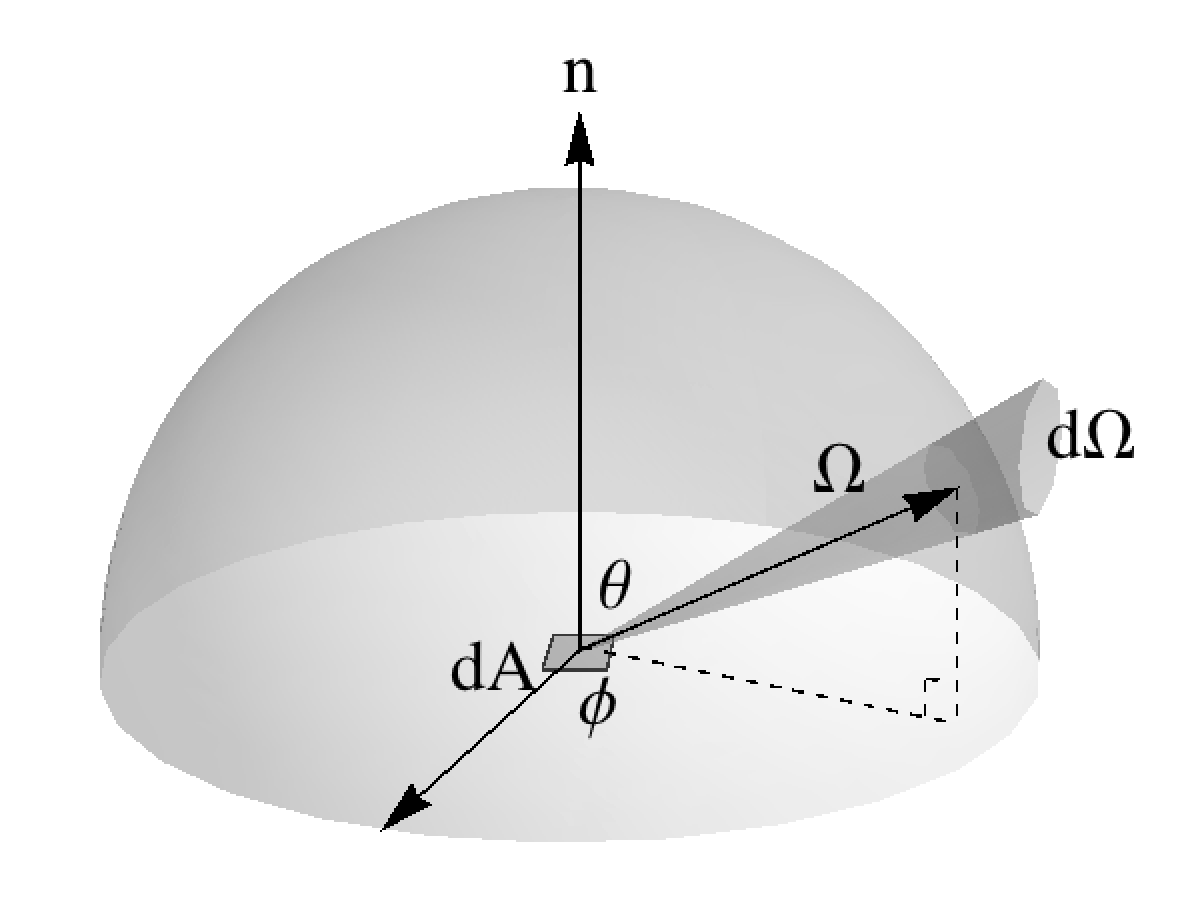
\includegraphics[width=\linewidth]{fig/radiance_bw.png}
	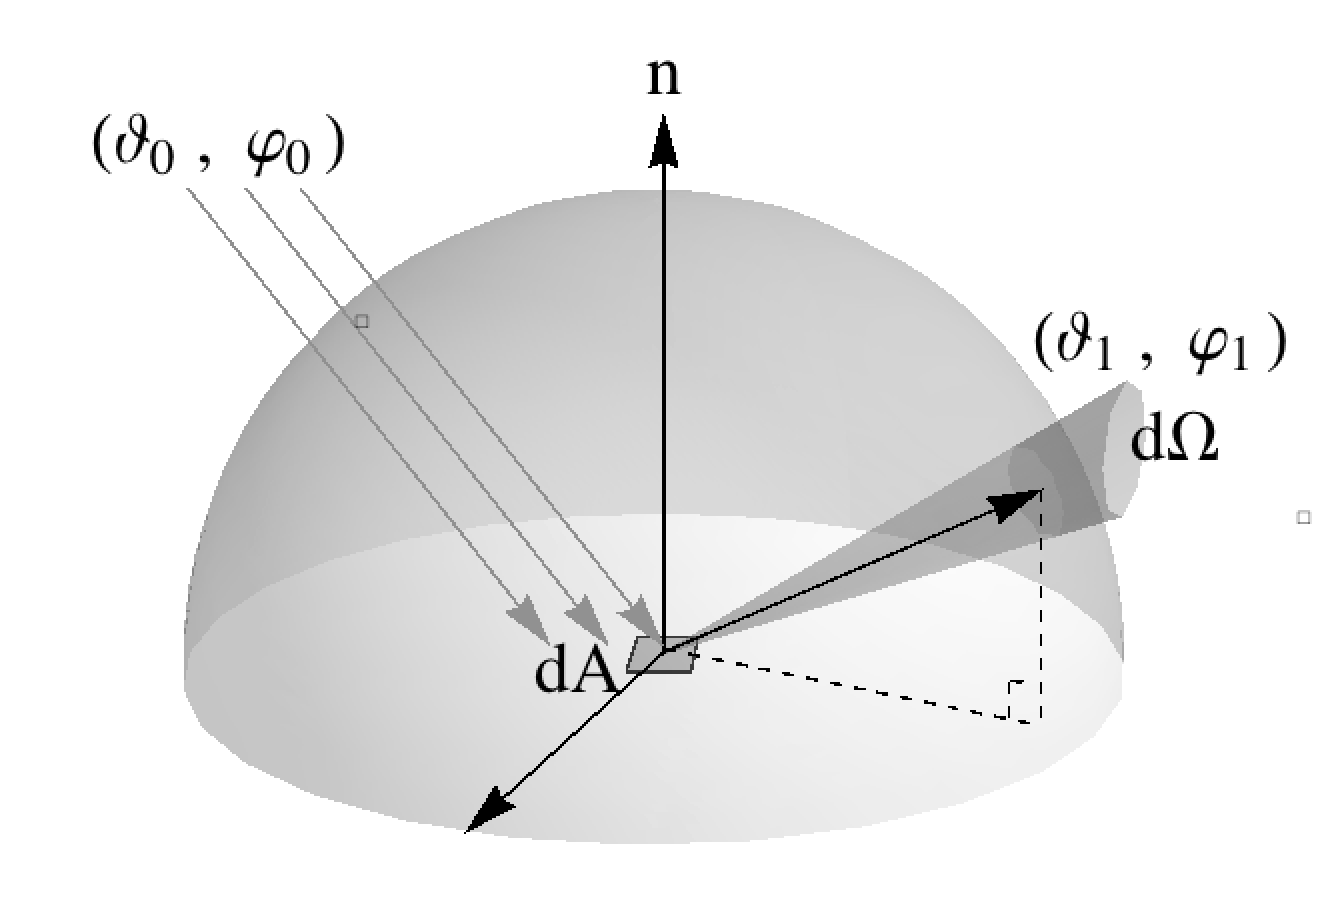
\includegraphics[width=\linewidth]{fig/brdfdef_bw.png}
\end{center}
	\caption{(上)素片$d A$からの放射または、素片への放射。(下)($\vartheta_0,\varphi_0$)方向からの平行光の入射と立体角$d \Omega$あたりの($\vartheta_0,\varphi_0$)方向への反射。}
	\label{fig:int}
\end{figure} 

\section{輻射スペクトル}

半径$R_p$で温度$T$の球から発する黒体輻射を距離$d$で測定した時のフラックスを考える。
温度$T$を持った表面は黒体輻射を行う。黒体輻射のRadianceは
\begin{align}
L_{\uparrow} d \lambda = B_\lambda (T) d \lambda = \frac{2 h c^2}{\lambda^5} \frac{1}{\exp{(hc/\lambda k_B T)}-1} d \lambda
\end{align}
でである。素片$d A$から$d \Omega$の放射コーンを考え、距離$d$にある面積$d A_\mathrm{tel}$の望遠鏡がコーンの先端と考える($d \Omega = d A_\mathrm{tel}/d^2$)と、$d A$から$d A_\mathrm{tel}$が受け取るエネルギー$\Delta E d A_\mathrm{tel}$は、
\begin{eqnarray}
\label{eq:brdfdef3}
\Delta E d A_\mathrm{tel} &=& L_\uparrow \cos{\vartheta_1} d \Omega d A \\
&=& \frac{L_\uparrow}{d^2} \cos{\vartheta_1} d A d A_\mathrm{tel}
\end{eqnarray}
となる。すなわち、観測者から見た素片$d A$によるIrradianceもしくはフラックスは
\begin{eqnarray}
\label{eq:brdfdef6}
\Delta E = \frac{L_\uparrow}{d^2} \cos{\vartheta_1} d A
\end{eqnarray}
となる。

これを全球で積分して、
\begin{align}
\label{eq:raddef}
f_p &= \int_\mathrm{planet} \Delta E = \int_\mathrm{planet} d A \frac{B_\nu (T)}{d^2} \cos{\vartheta_1} \\
&= R_p^2 B_\nu (T) \int_0^{2 \pi} d \varphi_1 \int_0^{\pi/2} d \vartheta_1 \sin{\vartheta_1} \cos{\vartheta_1}\\
&= \pi B_\nu (T) \frac{R_p^2}{d^2}
\end{align}
となる。全エネルギーは波長方向の積分と距離$d$の球殻面積をかけて
\begin{align}
\label{eq:raddeftot}
L &= 4 \pi d^2 \int_0^{\infty} d \nu \pi B_\nu (T) \frac{R_p^2}{d^2} = 4 \pi R_p^2 \sigma T^4  
\end{align}
となる。\\


惑星からの輻射スペクトルは第ゼロ近似では、単一温度$T_p$の黒体輻射
\begin{align}
f_p (\lambda) d\, \lambda  &= \pi B_\lambda(\lambda,T_p) \frac{ R_p^2}{d^2}  d \lambda \\
&= \frac{2 \pi h c^2}{\lambda^5} \frac{ R_p^2}{d^2} \left[ \exp{ \left(\frac{h c}{\lambda k_B T_p} \right) }- 1 \right]^{-1} d\, \lambda ,
\label{eq:planckdist}
\end{align}
で近似することができる場合がある。

例えば、ほぼ大気の存在しない地球の輻射スペクトルは、表面温度の$T=200--300$Kの黒体輻射でおおまかに近似できる。しかし、ガス惑星や褐色矮星に関しては、黒体輻射の近似はあまりよくない。これは大気中の分子の強い吸収によるところが大きい。放射スペクトルは、大気中の光学的厚さが1付近になる深さの大気層の黒体輻射に近い光によるが、これは大気中の分子により波長ごとに大きく変化する。この黒体輻射からの大きな破れが、系外惑星大気の特徴である。\\


\begin{itembox}{上向き射出フラックス}
\footnotesize
\color{gray}
大気の放射平衡モデルでは、大気高さ方向の一次元モデルのフラックスを考えるが、境界条件に地表のフラックスを与えることがある。同様にある黒体放射の素片から上向き射出されるフラックスを考えよう。素片周囲の上半面での角度積分を考えて
\begin{align}
\label{eq:defsurf}
F_\nu (T) &= \Delta E = \int_\mathrm{us} d \Omega B_\nu (T) \cos{\vartheta_1} = \pi B_\nu (T)
\end{align}
となる。全エネルギーでは同様に波長積分をして
\begin{align}
\label{eq:defsurflum}
F (T) &= \int d \nu f_\nu (T) = \sigma T^4 
\end{align}
となる。
\end{itembox}

\section{反射・散乱スペクトル}

反射光は、反射面・観測者との相対位置により観測される強度がことなるので若干複雑である。しかし平均的には以下のように考えることができる。まず、式(\ref{eq:lab})の時に、惑星が受け取らなかったエネルギーが反射となるので、反射のエネルギーは
\begin{align}
    L^\mathrm{ref}_p = A \pi R_p^2 S = \frac{L_\star}{4 \pi a^2} \pi R_p^2 A
\end{align}
である。距離$d$で受け取る反射フラックスは平均的には
\begin{align}
    \langle f_{p}^\mathrm{ref} \rangle = \frac{ L^\mathrm{ref}_p}{4 \pi d^2}
\end{align}
であるから、恒星のフラックス
\begin{align}
    f_\star = \frac{L_\star}{4 \pi d^2}
\end{align}
を用いて、
\begin{align}
    \langle f_{p}^\mathrm{ref} \rangle = \frac{A}{4} \left( \frac{R_p}{a} \right)^2 f_\star
\end{align}
となる。

スペクトルの観点からは、波長の関数となっているのは$A$と$f_\star$の掛け算、つまり恒星スペクトルに反射スペクトルがかかったものであるという点である。
\begin{align}
    \langle f_{p}^\mathrm{ref} \rangle (\lambda) d \lambda = \frac{1}{4} \left( \frac{R_p}{a} \right)^2 A(\lambda) f_\star (\lambda) d \lambda
\end{align}
である。

平均ではなく位相の関数としてフラックスを求めるのは少し複雑であるのでここでは割愛する。詳しくは拙著、系外惑星探査5.1.1を参照のこと。ここでは結果だけ紹介する。距離$d$の位置から観測した惑星の反射光フラックス$f_p^\mathrm{ref} (\lambda)$は、主星-惑星間距離$a$, 惑星アルベド$A(\lambda)$、惑星半径$R_p$、距離$d$から観測した主星フラックス$f_\star (\lambda)$、また観測者から見た惑星位置による関数$\phi (\beta)$を用いて
\begin{align}
\label{eq:refplanet}
f_p^\mathrm{ref} (\lambda) = \frac{2 \phi(\beta)}{3} A(\lambda) \left(\frac{R_p}{a}\right)^2 f_\star (\lambda),
\end{align}
\begin{align}
\label{eq:phaselambert}
\phi(\beta) \equiv [\sin{\beta} +  (\pi - \beta) \cos{\beta}]/\pi, 
\end{align}
と表される。ここで$\phi (\beta)$はLambert phase function\index{Lambert phase function@Lambert phase function}とよばれ、位相角(phase angle) $\beta = \angle $(主星ー惑星ー観測者)の関数である。ただしこの関係は、等方散乱を仮定していることに注意が必要である。海洋による鏡面反射(ocean glint)などの非等方性の強い反射では必ずしも成り立たない。

恒星光が惑星にあたって反射・散乱する光は、現在の技術では、宇宙からの精密測光での位相カーブとしての検出などの限定された条件でしか達成されていないが、原理的には惑星表面の二次元分布情報を持つ豊かな情報源である。反射光で重要な指標は主星と惑星のフラックス比、{\bf 主星惑星コントラスト}\index{しゅせいわくせいこんとらすと@主星惑星コントラスト}
\begin{align}
\label{eq:contrast}
c_{\mathrm{sp}} (\lambda) \equiv \frac{f_p (\lambda)}{f_\star (\lambda)}
\end{align}
である。主星惑星コントラストが緩いほうが直接撮像においても位相カーブにおいても検出が容易となる。

半月ならぬ半惑星($\beta=90^\circ$)の場合、式(\ref{eq:refplanet})を用いて、主星惑星コントラストを見積もることができる。地球の場合
\begin{align}
\label{eq:refplanetearth}
c_\mathrm{sp}  \approx 10^{-10} \left( \frac{A}{0.3} \right) \left(\frac{R_p}{R_\oplus} \right)^{2} \left(\frac{a}{1 \, \mathrm{au}} \right)^{-2}
\end{align}
程度に、ホットジュピターの場合
\begin{align}
\label{eq:refplanetearth}
c_\mathrm{sp}  \approx 10^{-6} \left( \frac{A}{0.1} \right) \left(\frac{R_p}{R_J} \right)^{2} \left(\frac{a}{0.05 \, \mathrm{au}} \right)^{-2}
\end{align}
程度になることがわかる。


\section{様々な系外惑星スペクトル}



図\ref{fig:earth}は地球のスペクトルである。地球の場合、大気が薄いので輻射光はほぼ放射平衡温度に近い黒体となっている。また反射スペクトルは恒星スペクトルに大気吸収がかかったものとなっている。

図\ref{fig:bd}は褐色矮星のスペクトル。黒体から大きく外れている。

図\ref{fig:jwst}はJWST NIRSPECによるホットサターンWASP-39bのスペクトルである。分子吸収によるfeatureが見て取れる。


\begin{figure}[]
 \begin{center}
	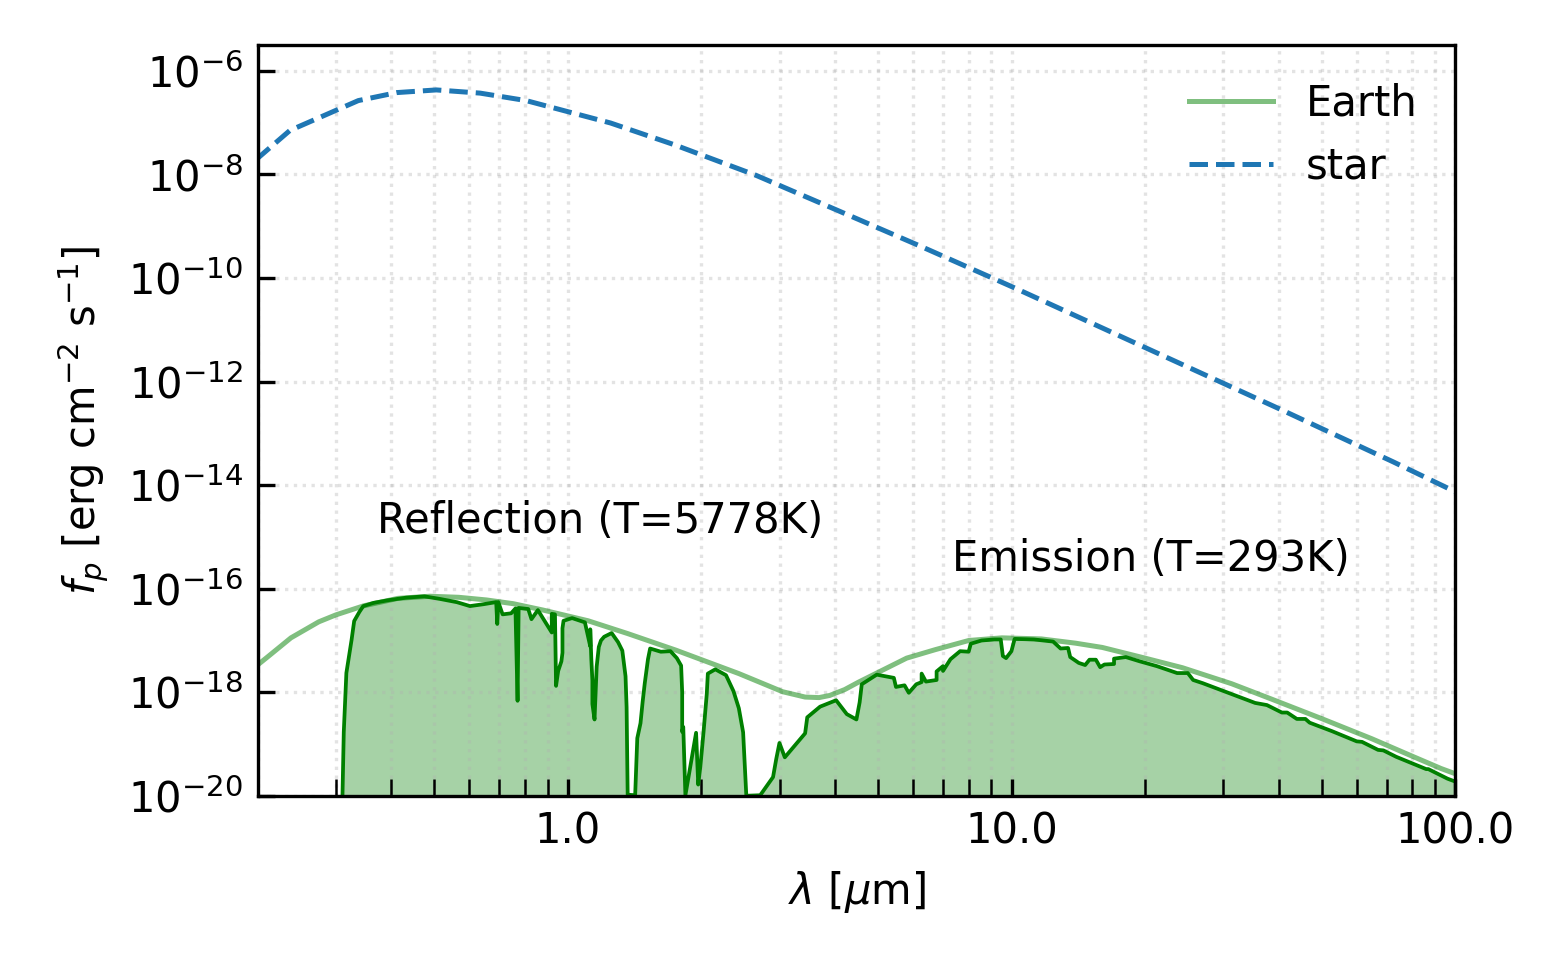
\includegraphics[width=\linewidth]{fig/EarthEmis.png}
\end{center}
	\caption{地球のスペクトル}
	\label{fig:earth}
\end{figure} 

\begin{figure}[]
 \begin{center}
	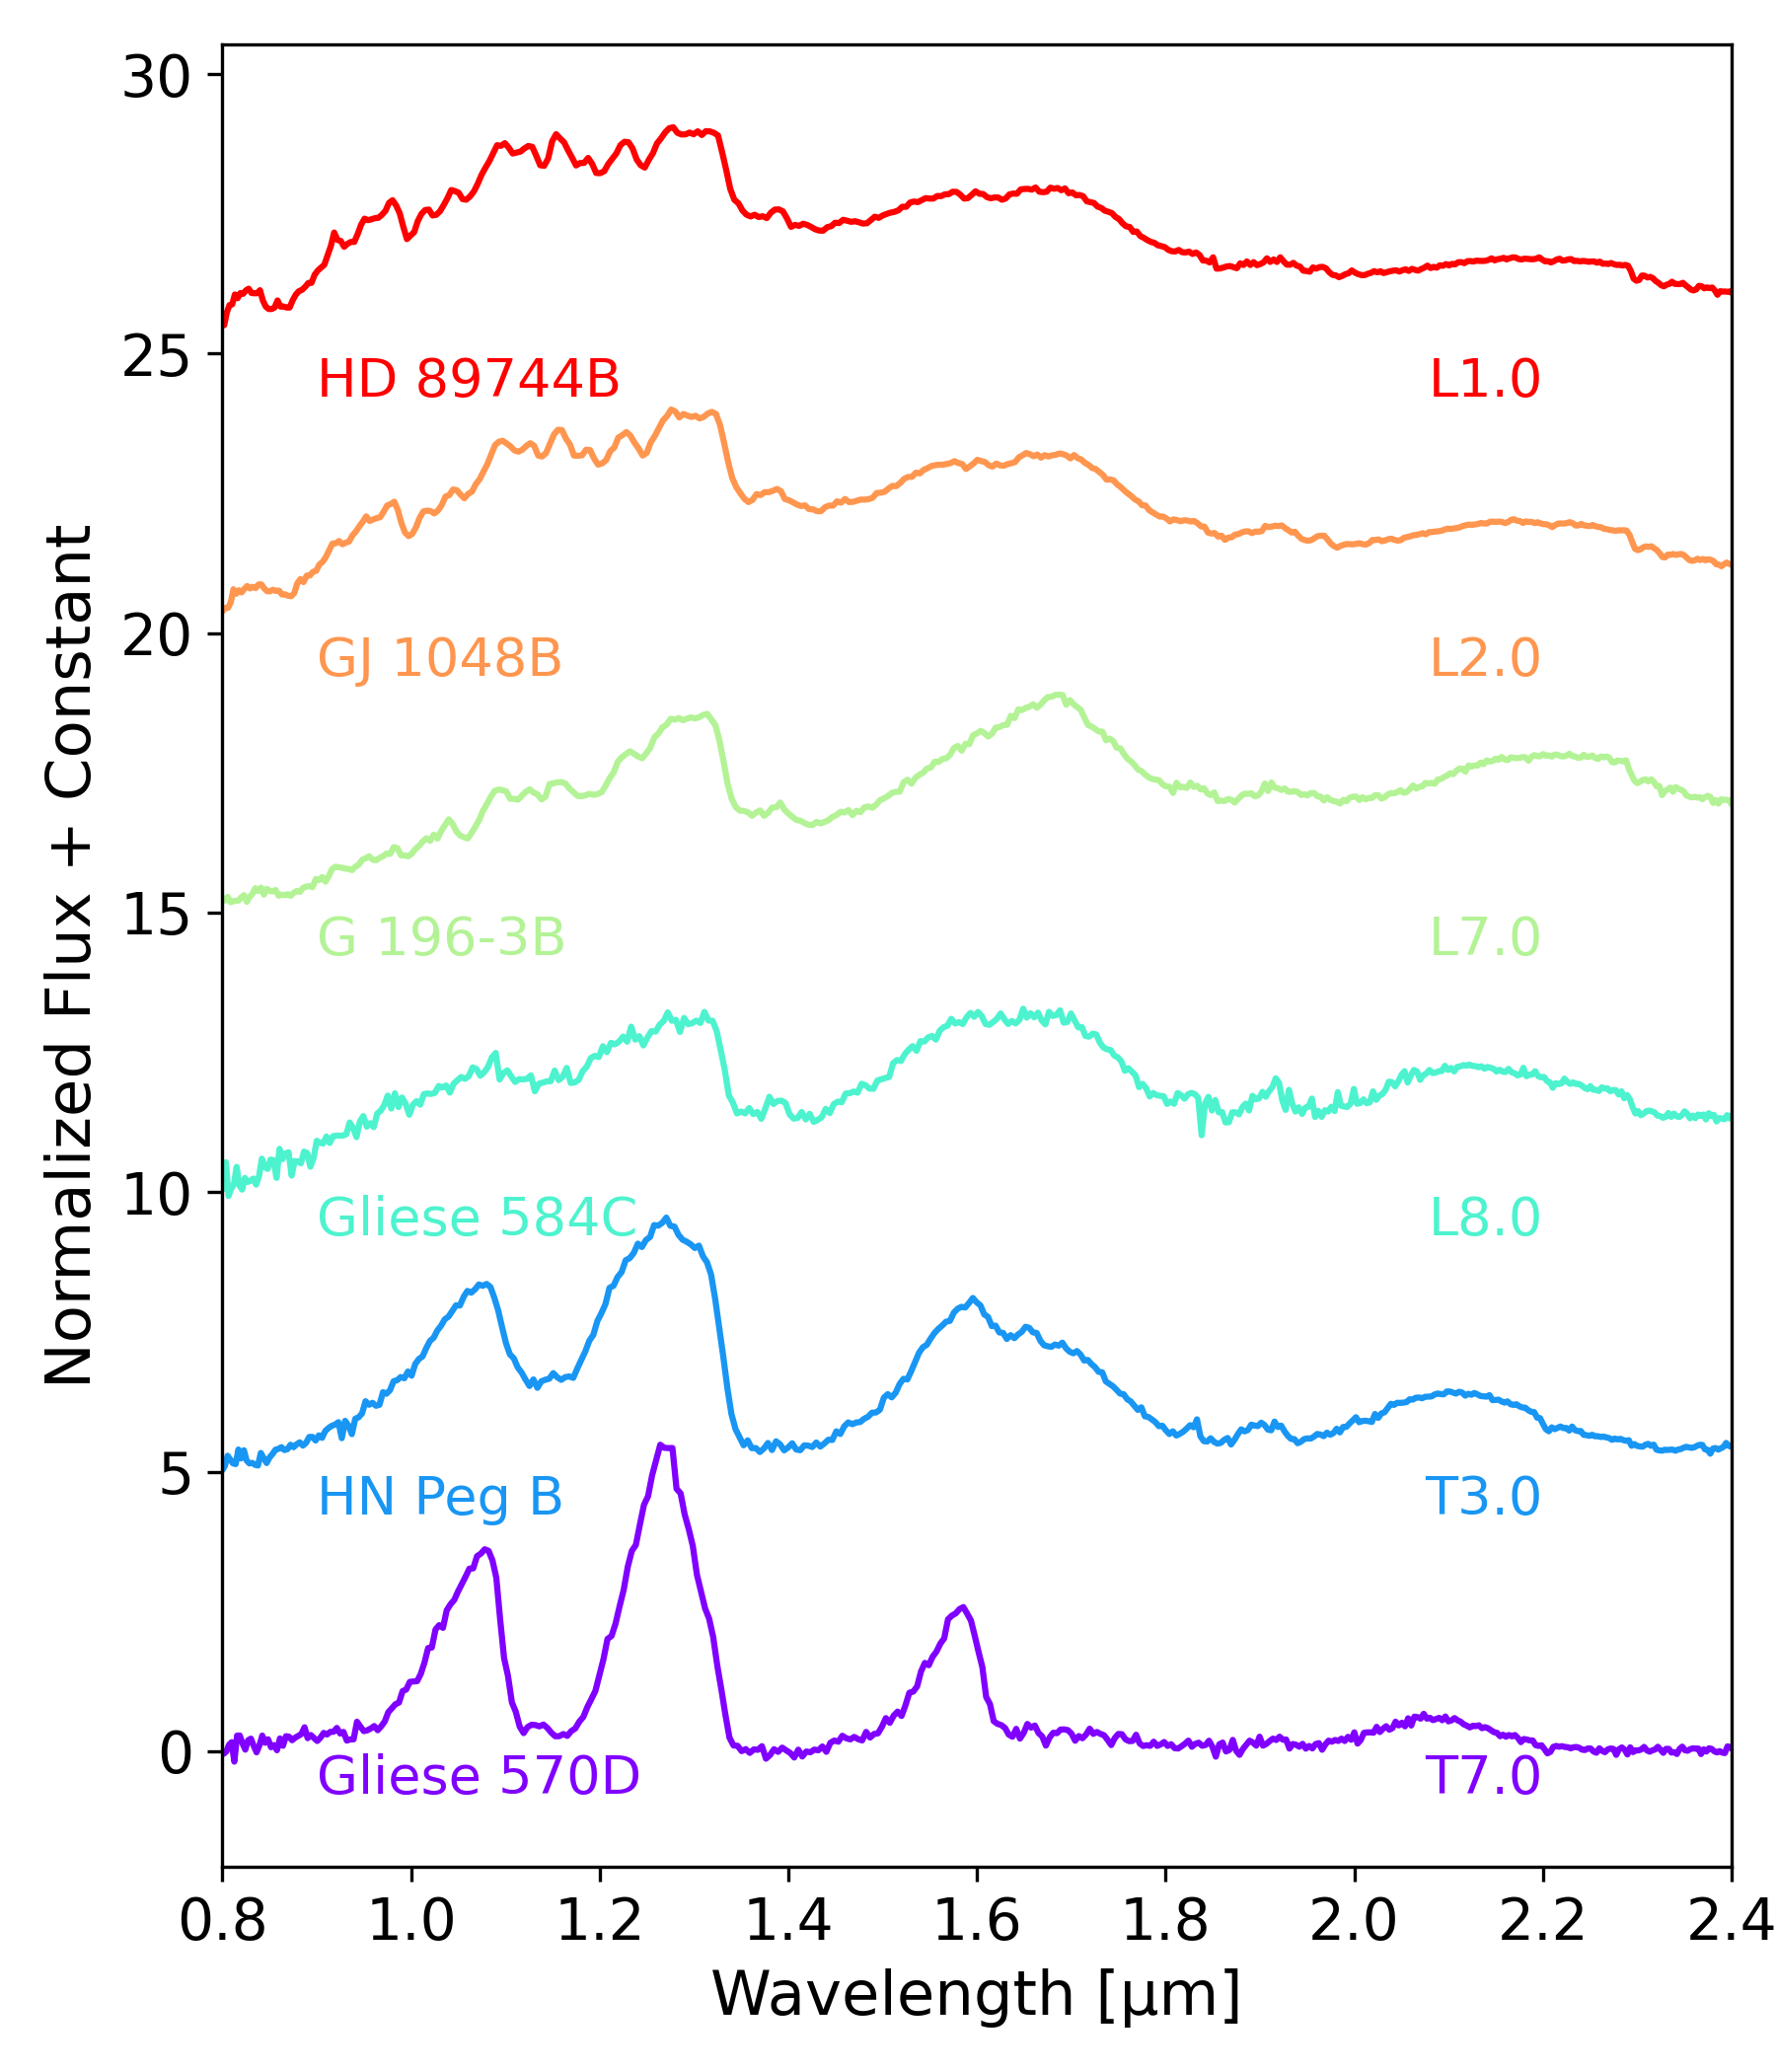
\includegraphics[width=\linewidth]{fig/bdspectra.png}
\end{center}
	\caption{褐色矮星のスペクトル (SpeX Prismライブラリー) Inspired by\cite{2025ApJ...988...31L}}
	\label{fig:bd}
\end{figure} 


\begin{figure*}[htb]
 \begin{center}
	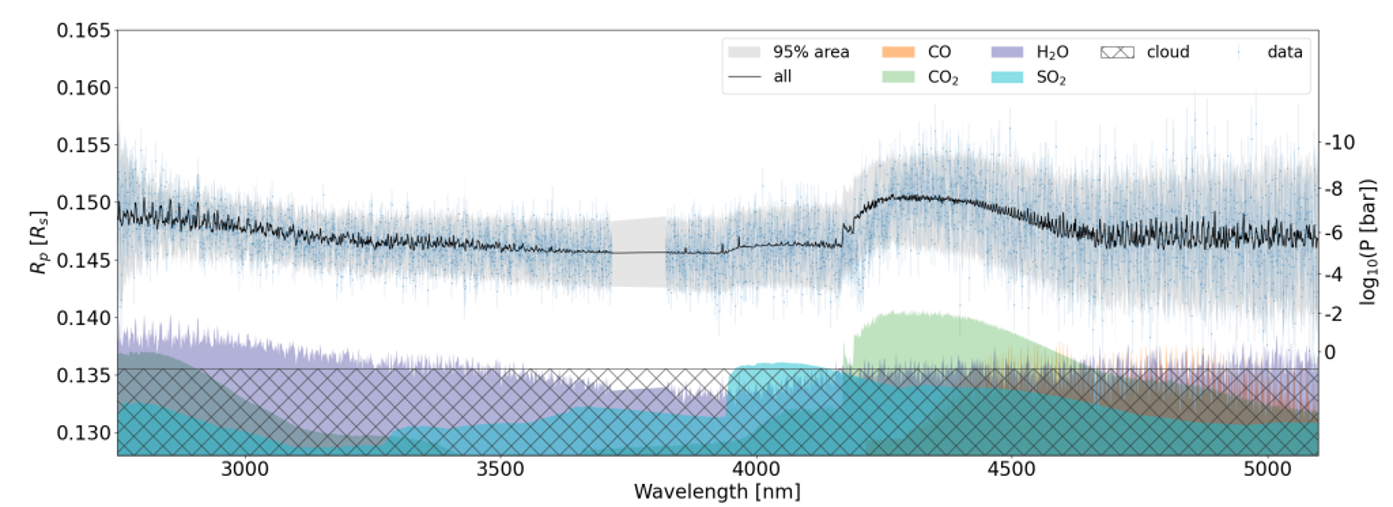
\includegraphics[width=\linewidth]{fig/jwst_spectrum.png}
\end{center}
	\caption{JWST透過光スペクトル WASP-39 b \cite{2025ApJ...985..263K}}
	\label{fig:jwst}
\end{figure*} 



%\input{} direct


\chapter{系外惑星大気}
\section{熱化学平衡における分子混合率}

系外惑星大気中の分子の存在量は、高温高圧の場合は熱化学平衡に近づくと考えられる。鉛直輸送や光化学反応、もしくは低温系大気の場合あっても、熱化学平衡の時にどうなるかは一つの基準として知っておくべきである。
そこで、ここでは熱化学平衡に至っている場合の大気中の分子中の混合率がどのように決定されるか考える。\\

\subsection*{元素の保存}

ガス中には\ce{H2}や\ce{H}、\ce{H2O}をいった分子種や原子種、イオン、自由電子が適当な割合で混合している。これらをまとめて{\bf 種}(species)と呼ぶ。これら大気種中に含まれる原子の総数を考えたい。ガス中に含まれる種の中の原子(例えば\ce{H, O, C})ではなく、ガス中のすべての分子や原子に含まれる原子を{\bf 元素}(elements)と呼び区別する。本文書では元素をサンセリフ体を用いて、$\Hel$, $\Oel$, $\Cel$のようにあらわす。\\

\subsection*{二成分系の場合}

まず最も単純な以下の水素原子と水素分子のガス2成分系
\begin{align*}
\ce{2 H <--> H2}
\end{align*}
の場合、熱化学平衡でどのような組成比になるかを考えてみよう\footnote{実際は少量の触媒Mを介して\ce{2 H + M <--> H2 + M}としたほうが現実的だが、ここでは数学的側面を重視しMを無視する。}。この場合、種は\ce{H}と\ce{H2}の二種類($N_s = 2$)であり、元素は$\Hel$の一種類($N_e = 1$)である。

いま元素量として$\nel_{\Hel}$(例えば1 mol)の水素を考える。すなわち元素保存則は
\begin{align}
    n_\mathrm{H} + 2 n_\mathrm{H2}  = \nel_{\Hel} 
\end{align}
となる。圧力$P$と温度$T$を与えたときに、熱化学平衡条件を満たす場合に、この元素$\Hel$がどのように\ce{H}と\ce{H2}に分配されるかを与えるのが、ギブス自由エネルギーの最小化である。すなわち熱化学平衡においては種の存在量は以下の最小化で与えられる
\begin{align}
\label{eq:opt1tce}
    &(n_\mathrm{H}^\ast, n_\mathrm{H2}^\ast) = \mathrm{minimize}_{(n_\mathrm{H}, n_\mathrm{H2})} \,\, G(T, P, n_\mathrm{H}, n_\mathrm{H2}) \,\, \\ 
    &\mbox{subject to} \,\, n_\mathrm{H} + 2 n_\mathrm{H2} =  \nel_{\Hel}  \\
    &G(T, P, n_\mathrm{H}, n_\mathrm{H2}) = n_\mathrm{H} \mu_\mathrm{H} + n_\mathrm{H2} \mu_\mathrm{H2} \\
     &\, n_\mathrm{H} \ge 0, n_\mathrm{H2} \ge 0
\end{align}
ここに$\mu_\mathrm{H}$、$ \mu_\mathrm{H2}$は\ce{H}, \ce{H2}の化学ポテンシャルであり、標準状態の化学ポテンシャルを用いると
\begin{align}
    \mu_\mathrm{H} &= \mu_\mathrm{H}^o(T) + RT \log{\frac{P_\mathrm{H}}{P_\mathrm{ref}}} \\
    &=  \mu_\mathrm{H}^o(T) + RT \log{\frac{n_\mathrm{H} P}{(n_\mathrm{H} + n_\mathrm{H2}) P_\mathrm{ref}}} \\
    \mu_\mathrm{H2} &= \mu_\mathrm{H2}^o(T) + RT \log{\frac{P_\mathrm{H2}}{P_\mathrm{ref}}} \\
    &=  \mu_\mathrm{H2}^o(T) + RT\log{\frac{n_\mathrm{H2} P}{(n_\mathrm{H} + n_\mathrm{H2}) P_\mathrm{ref}}}
\end{align}
で与えられる。$\partial G/\partial n_\mathrm{H} = \mu_\mathrm{H}$, $\partial G/\partial n_\mathrm{H2} = \mu_\mathrm{H2}$が満たされることを確認せよ。

ここでは後の一般化を考え、上の等式条件付き最適化をラグランジュ未定乗数法で解く。ラグランジュ未定乗数法では、自由パラメタを$\xv = ( n_\mathrm{H},  n_\mathrm{H2}, \lambda )^\top$の3パラメタとして
\begin{align}
\label{eq:opt2tce}
    \xv_\ast &= \mathrm{minimize}_{\xv} \,\, \mathcal{L} (T, P, \xv) \\ 
    \mathcal{L} (T, P, \xv) &\equiv G(T, P, \xv) + \lambda (n_\mathrm{H}  + 2 n_\mathrm{H2} - \nel_{\Hel} ) \\
    \label{eq:nonnegative_tce}
    &n_\mathrm{H} \ge 0, n_\mathrm{H2} \ge 0
\end{align}
を解けばよい。最後の非負条件は後でチェックする。$\mathcal{L} (T, P, \xv)$を$\xv$で偏微分したものが$\boldsymbol{0}$であるとして、$\xv=\xv_\ast$を求める。すなわち
\begin{align}
&\frac{\partial \mathcal{L} (T, P, \xv)}{\partial \xv} = 
\begin{pmatrix}
    \mu_\mathrm{H} + \lambda \\
    \mu_\mathrm{H2} + 2 \lambda \\
    n_\mathrm{H} + 2 n_\mathrm{H2} -  \nel_{\Hel} 
\end{pmatrix}\\
&=
\displaystyle{
\begin{pmatrix}
    \mu_\mathrm{H}^o(T) + RT \log{\frac{n_\mathrm{H} P}{(n_\mathrm{H} + n_\mathrm{H2}) P_\mathrm{ref}}}  + \lambda \\
    \mu_\mathrm{H2}^o(T) + RT\log{\frac{n_\mathrm{H2} P}{(n_\mathrm{H} + n_\mathrm{H2}) P_\mathrm{ref}}} + 2 \lambda \\
    n_\mathrm{H} + 2 n_\mathrm{H2} -  \nel_{\Hel} 
\end{pmatrix}
}
=
\begin{pmatrix}
    0 \\
    0 \\
    0
\end{pmatrix}
\end{align}
である。第1,2成分から$\lambda$について消去すると
\begin{align}
    \log{\left( \frac{n_\mathrm{H}^2 }{n_\mathrm{H2} (n_\mathrm{H} + n_\mathrm{H2})} \frac{P}{P_\mathrm{ref}} \right)} =- \frac{2 \mu_\mathrm{H}^o - \mu_\mathrm{H2}^o}{RT} 
\end{align}
がえられる。第3成分(保存則)$n_\mathrm{H} + 2 n_\mathrm{H2} - \nel_{\Hel}=0$をもちいて、$n_\mathrm{H2}$を消去すると、
\begin{align}
\frac{ \nel_{\Hel}^2 - n_\mathrm{H}^2}{4 n_\mathrm{H}^2} = \frac{P}{P_\mathrm{ref}} 
\exp{\left( - \frac{\mu_\mathrm{H2}^o - 2 \mu_\mathrm{H}^o}{RT} \right)}  \equiv k
\end{align}
であり、$n_\mathrm{H} \ge 0$より
\begin{align}
 \frac{n_\mathrm{H}}{ \nel_{\Hel} } = \frac{1}{\sqrt{4 k + 1}}
\end{align}
また保存則より
\begin{align}
 \frac{n_\mathrm{H2}}{ \nel_{\Hel} } = \frac{1}{2} \left( 1 - \frac{1}{\sqrt{4 k + 1}} \right)
\end{align}
となる。これらは水素元素$\nel_{\Hel}$あたりの分子量となっていることに注意する。つまり実務上は$\nel_{\Hel}=1$ (mol)ととって計算を進めてもよい。

また体積分率(Volume Mixing Ratio)は
\begin{align}
 \mathrm{VMR} (\ce{H}) &= \frac{n_\mathrm{H}}{n_\mathrm{tot}} = \frac{1}{2} \left( \sqrt{k^2 + 4 k} - k \right) \\
  \mathrm{VMR} (\ce{H2}) &= \frac{n_\mathrm{H2}}{n_\mathrm{tot}} = \frac{1}{2} \left( 2 + k - \sqrt{k^2 + 4 k}\right)
\end{align}
となる。図\ref{fig:temperature_exogibbs}に混合率の温度依存性を図示した。

\begin{figure}
    \centering
    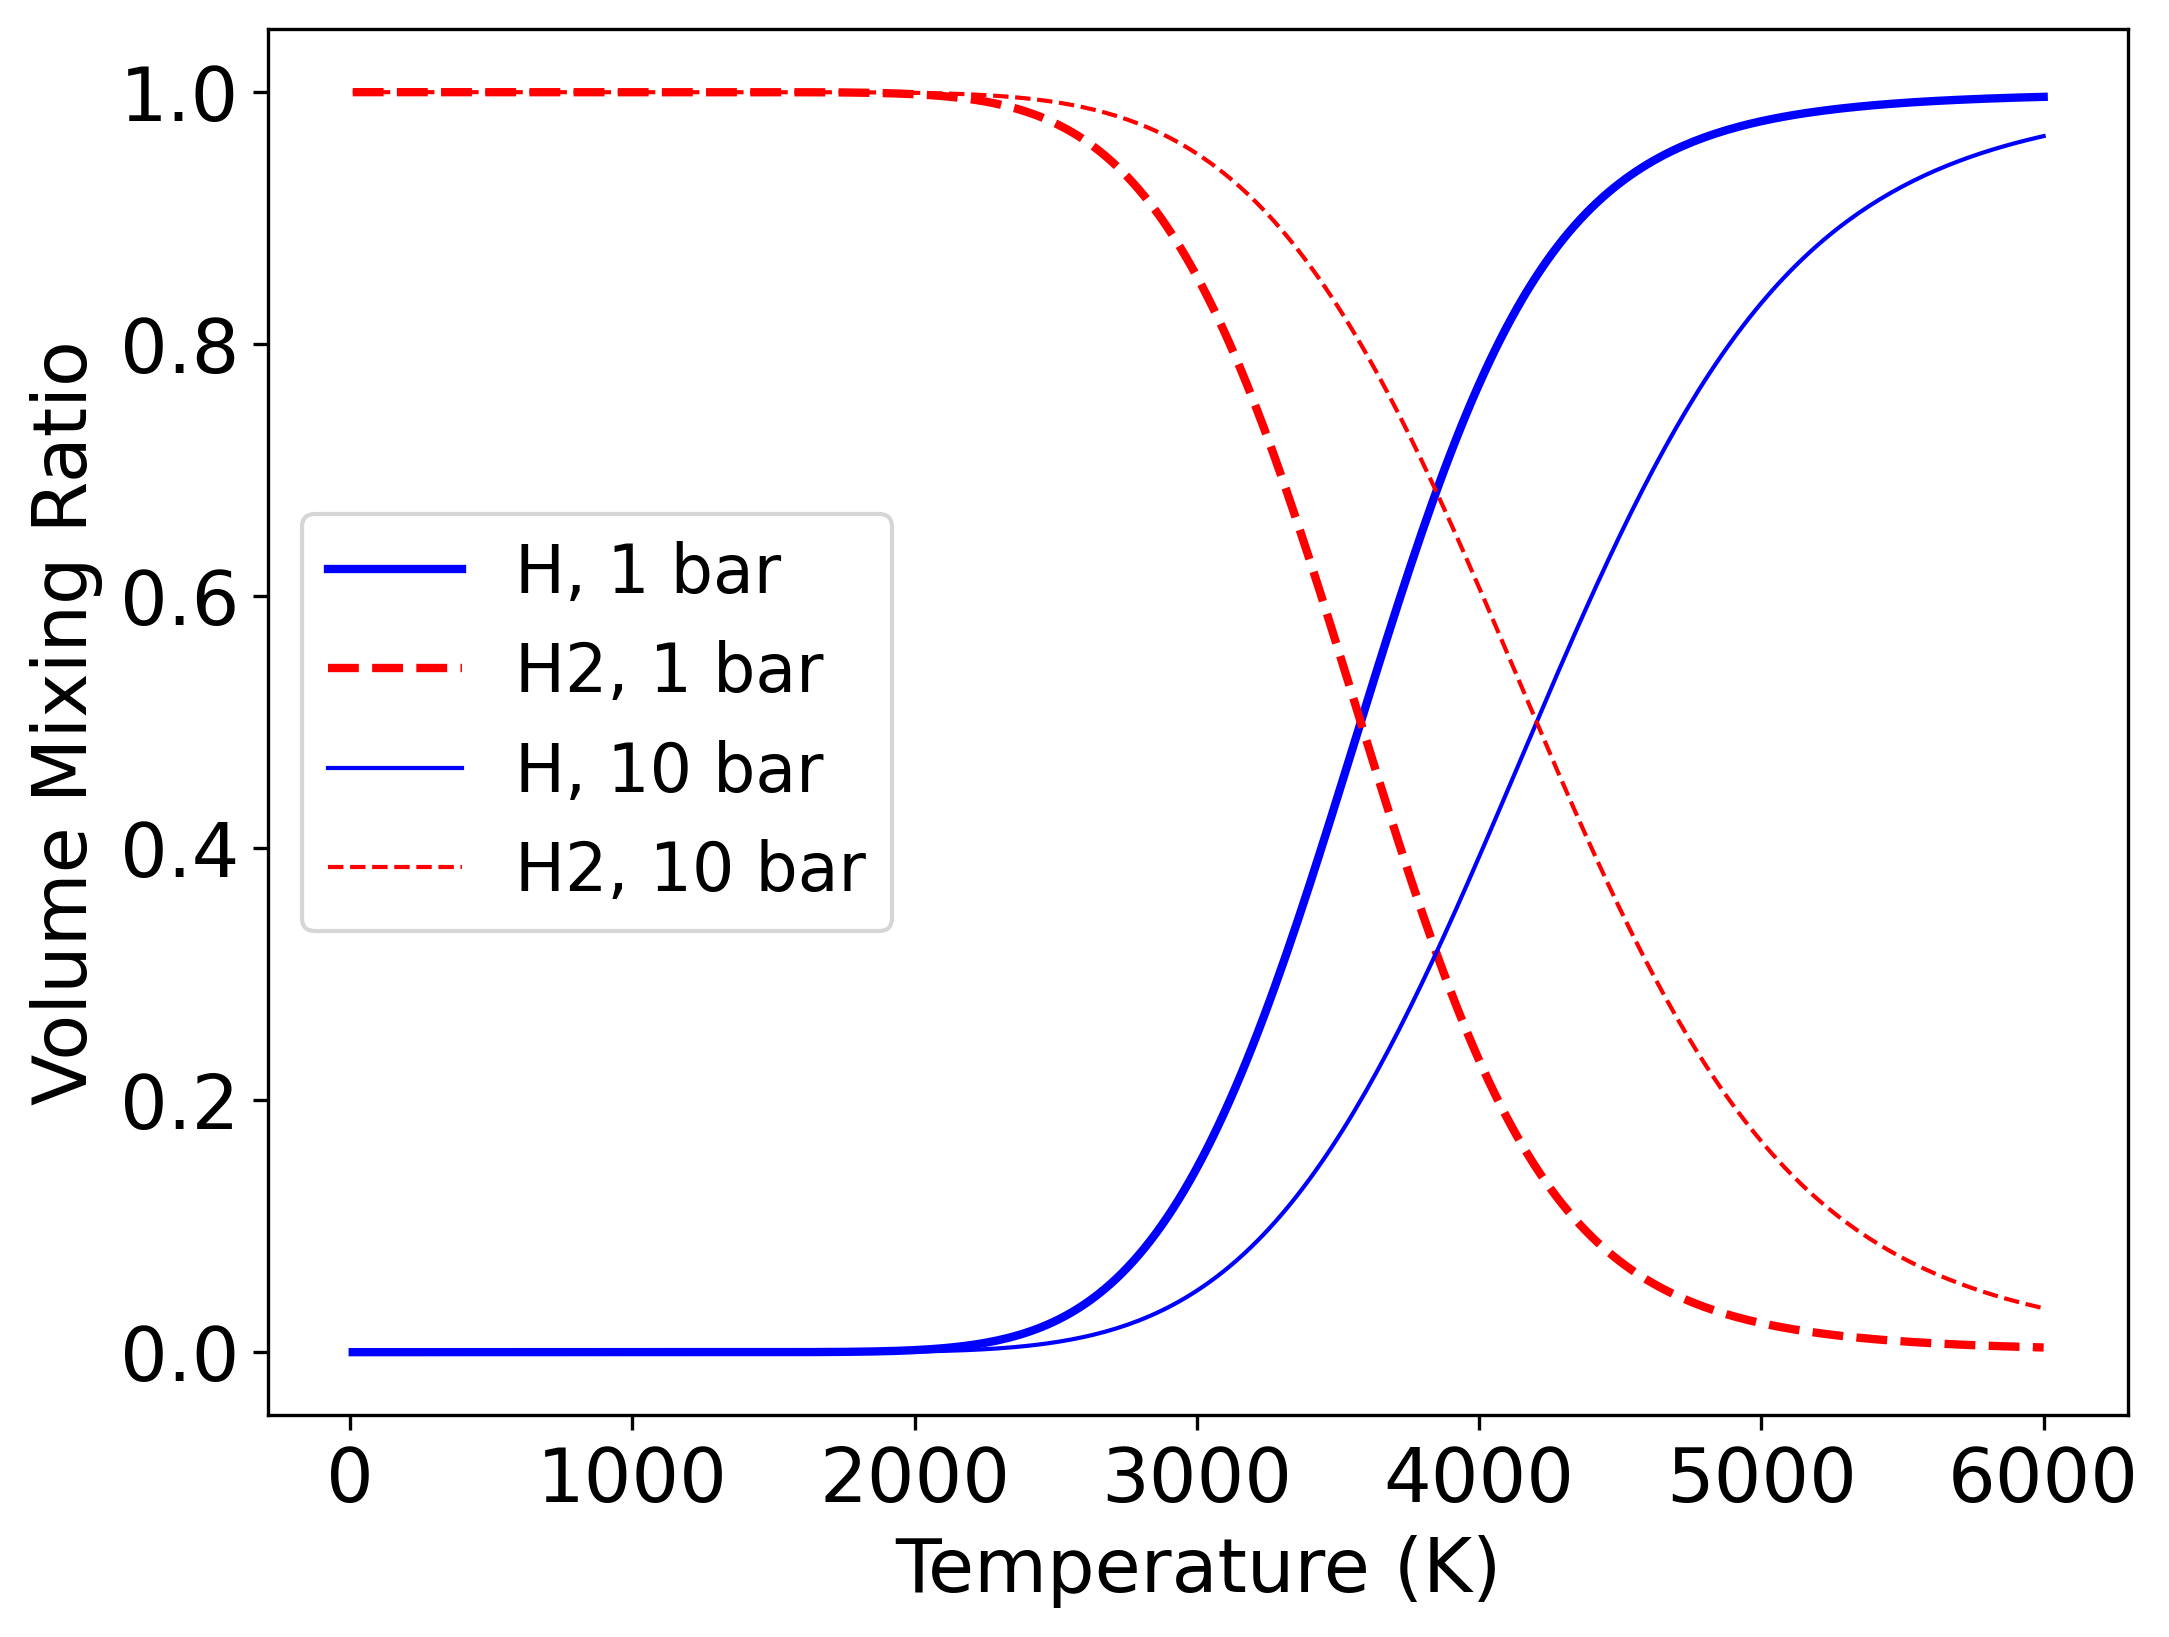
\includegraphics[width=\linewidth]{fig/tce_two_species.png}
    \caption{\ce{2 H <--> H2}の熱化学平衡の体積混合率}
    \label{fig:temperature_exogibbs}
\end{figure}

\subsection*{多成分系の場合$^\ddagger$}

次に多元素系を考える. 
今,例として元素として$\Hel, \Cel, \Oel$,また種としては\ce{CO, H2, CH4, H2O}からなる系を考えよう. これらは水素大気の分子成分としては主要なものである. 化学反応としては以下の一つの反応式となる. 
\begin{align*}
\ce{CO + 3 H2 <--> CH4 + H2O}
\end{align*}
となる. 


要素との化学反応式を考えると,
\begin{align*}
\ce{H2 <--> 2 $\Hel$ \, \, \, \, \, \, \, \, \\
H2O <--> 2 $\Hel$ + 1 $\Oel$ \\
CH4 <--> 4 $\Hel$ + 1 $\Cel$ \\
CO <-->  1 $\Cel$ + 1 $\Oel$
}
\end{align*}
のようになる. ここで,0成分も含んで表現すると
\begin{align*}
\ce{H2 <--> 2 $\Hel$ + 0 $\Cel$ + 0 $\Oel$ \\
H2O <--> 2 $\Hel$ + 0 $\Cel$ + 1 $\Oel$ \\
CH4 <--> 4 $\Hel$ + 1 $\Cel$ + 0 $\Oel$ \\
CO <--> 0 $\Hel$ + 1 $\Cel$ + 1 $\Oel$ \\ 
}
\end{align*}
のようになる. 右辺についてformula matrixを以下のように定義する. 
\begin{align*}
  A \equiv
\begin{pmatrix} 
2 & 2 & 4 & 0 \\
0 & 0 & 1 & 1 \\
0 & 1 & 0 & 1 
\end{pmatrix}  
\end{align*}

種の存在量ベクトルを$\nv = (n_\mathrm{H_2}, n_\mathrm{H_2 O},n_\mathrm{C H_4},n_\mathrm{CO})^\top$,元素の存在量ベクトルを$\bv = (\nel_\Hel, \nel_\Cel, \nel_\Oel)^\top$と置くと(元素の存在量を種とは区別している点に注意),元素保存則は
\begin{align}
    A \, \nv = \bv 
\end{align}
と表されることが分かる. 


多元素系でも同様に,以下のGibbsエネルギーを最小化すればよい
\begin{align}
\label{eq:gibss_multi}
    \nv^\ast &= \mathrm{minimize}_{\nv} G(T, p, \nv) \nonumber \\
    &\mbox{subject to} \,\, A \, \nv = \bv, n_i \ge 0\\
    G(T, p, \nv) &\equiv  \muv (T, p, \nv)^\top \nv\\ 
    \label{eq:chemical_potential_mu}
    \muv (T, p, \nv) &=  \muv^\circ(T) + RT \log{\left(\frac{p}{\ntot} \nv\right)} 
\end{align}
ただし総数密度と規格化圧力を
\begin{align}
\label{eq:ntot_tce}
    \ntot &= \sum_i n_i \\
    p &\equiv P/P_\mathrm{ref}
\end{align}
と定義した. 

\ce{CO, H2, CH4, H2O}系において, 式(\ref{eq:gibss_multi})は,
\begin{align}
    \mathcal{L}(T, p, \nv,\lambdav) &= \sum_{i = \ce{CO, H2, CH4, H2O}} \mu_i (T) \, n_i \nonumber \\ &+ \lambda_{\Hel} (2 n_{\ce{H2}} + 4 n_{\ce{CH4}} + 2 n_{\ce{H2O}} - b_\Hel) \nonumber \\
    &+ \lambda_{\Cel} (n_{\ce{CO}} + n_{\ce{CH4}} - b_\Cel) \nonumber \\ 
    &+  \lambda_{\Oel} ( n_{\ce{CO}} + n_{\ce{H2O}} - b_\Oel)
\end{align}

ここではGordon and McBrideによるNASA/CEA (Chemical Equilibrium with Applications)の実装法を元に解説する\cite{gordon1994computer,2024arXiv241207166G}. CEAではLagrange multiplierを用いてGibbsエネルギー最小化を行う二次の手法の一つである. すなわち
\begin{align}
    (\nv^\ast, \lambdav^\ast)  &= \mathrm{minimize}_{(\nv,\lambdav)} \,\, \mathcal{L}(T, p, \nv, \lambdav) \\
    \mathcal{L}(T, p, \nv,\lambdav) &= G(T, p, \nv) + \lambdav^\top \left(A \nv - \bv\right)  
\end{align}
を最小化する. ただしこの時点では非負条件$n_i \ge 0$は外れていない. 

$\mathcal{L}(T, p, \nv, \lambdav)$の停留点を求めるために,最適化変数のセット$\yv = (\nv, \lambdav)$で一次偏微分した関数を
\begin{align}
\label{eq:fv_tea0}
    \fv(\yv) &\equiv \frac{\partial  }{\partial \yv} \mathcal{L}(T, p, \yv) 
\end{align}
を定義する. そして
\begin{align}
    \label{eq:fv_tea}
    \fv(\yv^\ast) = \boldsymbol{0}
\end{align}
の解をNewton法でもとめることで,$\yv^\ast = (\nv^\ast, \lambdav^\ast)$を求める. 次に式(\ref{eq:fv_tea0})の$\nv$成分を計算する
\begin{align}
\label{eq:Lpartialn}
    \frac{\partial}{\partial \nv}   \mathcal{L}(T, p, \nv, \lambdav) =  \muv (T, p, \nv) + A^\top \lambdav  
\end{align}
ここに熱力学より$\partial_{\nv} G(T, p, \nv) =  \muv (T, p, \nv)$\footnote{式(\ref{eq:chemical_potential_mu})を用いて直接確かめることができる. }および$\lambdav^\top (A \nv) = (A^\top \lambdav)^\top \nv$と$\partial_{\xv} (S^\top \xv) = S$を利用した. 
式(\ref{eq:Lpartialn})は$\lambdav$について一次である点に注意する. $\lambdav$成分は単に保存関係
\begin{align}
\label{eq:Lpartiall}
\frac{\partial}{\partial \lambdav}  \mathcal{L}(T, p, \nv, \lambdav) = A \nv - \bv  
\end{align}
である. 

式(\ref{eq:chemical_potential_mu})を用いるとNewton法で解くべき方程式系(\ref{eq:fv_tea})は
\begin{align}
\label{eq:Lpartialnx}
    \frac{\muv^\circ(T)}{RT}+ \log{\left(\frac{p}{\ntot^\ast} \nv^\ast \right)} + \frac{A^\top \lambdav^\ast}{RT}   &= \boldsymbol{0} \\
    A \nv^\ast - \bv &= \boldsymbol{0}
\end{align}
となる. ただし$\ntot^\ast$は$\nv^\ast$の関数,すなわち
\begin{align}
\ntot^\ast &= \sum_i n_i^\ast
\end{align}
となる. 


ここでCEAのアルゴリズムではいくつかのトリックを用いる. まず,式(\ref{eq:fv_tea})を求めるために,独立変数に$\ntot$を追加する. もともと$\ntot$は式(\ref{eq:ntot_tce})により$\nv$に依存していたため,この条件,つまり式(\ref{eq:ntot_tce})を,(前提条件ではなく)制約条件として追加する. さらに$\nv$, $\ntot$は対数を取ったものを独立変数に取り直す. つまり$\lnnv = \ln{\nv}$, $\lnntot = \ln{\ntot}$を独立変数とする.  この操作により非負条件$n_i \ge 0$は自然に取り除かれる. また対数を取ることで広いダイナミックレンジで安定し
た数値計算となる. これにより新たな変数系として$\zv = (\lnnv, \lambdav, \lnntot)$が導入され,解くべき方程式は
\begin{align}
\label{eq:Lpartialncea}
    \Fv_n (\zv) &\equiv \frac{\muv^\circ(T)}{RT} + \lnnv - \lnntot \, \uv_\ngas + \log{p} \, \uv_\ngas  + \frac{A^\top \lambdav}{RT} = \boldsymbol{0}_\ngas \\
    \Fv_\lambda (\zv) &\equiv A e^{\lnnv} - \bv = \boldsymbol{0}_\nelements \\
    F_\mathrm{tot} (\zv) &\equiv \sum_i {e^{q_i}} - e^{\lnntot} = 0
\end{align}
である. $\boldsymbol{0}_\nelements$は$\nelements$次元ゼロベクトルである. この解が$\zv^\ast = (\lnnv^\ast, \lambdav^\ast, \lnntot^\ast)$となる. これを簡潔に$\Fv (\zv) = (\Fv_n (\zv), \Fv_\lambda (\zv), F_\mathrm{tot} (\zv))$とまとめて扱うこともある.  $\uv_\ngas$は$\ngas$次元 one vector.

Newton法では$\Fv (\zv)$を$\zv$で微分したヤコビアンが必要となる. 
\begin{align}
\label{eq:jacobian_tce}
\Jv (\zv) &=
\left(
\begin{array}{ccc}
    \dfrac{\partial \Fv_n}{\partial \lnnv}  & \dfrac{\partial \Fv_n}{\partial \lambdav}& \dfrac{\partial \Fv_n}{\partial \lnntot}\\ 
    \dfrac{\partial \Fv_\lambda}{\partial \lnnv} & \dfrac{\partial \Fv_\lambda}{\partial \lambdav} & \dfrac{\partial \Fv_\lambda}{\partial \lnntot} \\
    \dfrac{\partial F_\mathrm{tot}}{\partial \lnnv} & \dfrac{\partial F_\mathrm{tot}}{\partial \lambdav} & \dfrac{\partial F_\mathrm{tot}}{\partial \lnntot} \\  
\end{array}
\right) \nonumber \\
&=
\left(
\begin{array}{ccc}
 E_\ngas &  \dfrac{A^\top}{RT} & - \uv_\ngas\\ 
 Y(\lnnv) & Z_\nelements & \boldsymbol{0}_\nelements \\ 
 (e^{\qv})^\top & \boldsymbol{0}_\nelements^\top & - e^\lnntot\\  
\end{array}
\right)
\end{align}
となる. ここに
$E_\ngas$は$\ngas \times \ngas$単位行列,$Z_\nelements$は$\nelements \times \nelements$ゼロ行列, $\nelements$は元素ベクトル$\bv$の要素数である. また行列$Y(\lnnv)$は
$Y(\lnnv)= A \, \mathrm{diag}(e^{\lnnv}) $のことであり,すなわち要素が
\begin{align}
Y_{ij} = A_{ij} e^{q_j}
\end{align}
であるような行列である. Newton法のupdateは式(\ref{eq:second_newton})より,$\Jv (\zv_k) \Delta \zv = - \Fv (\zv_k)$をみたすので
\begin{align}
    \left(
\begin{array}{ccc}
 E_\ngas &  \dfrac{A^\top}{RT} & - \uv_\ngas\\ 
 Y({\lnnv}_k) & Z_\nelements & \boldsymbol{0}_\nelements \\ 
 (e^{{\lnnv}_k})^\top & \boldsymbol{0}_\nelements^\top & - e^{(\lnntot)_k}\\  
\end{array}
\right)
    &\left(
\begin{array}{c}
\Delta \lnnv \\
\Delta \lambdav \\
\Delta \lnntot
\end{array}
\right) \nonumber \\
= -
    &\left(
\begin{array}{c}
\Fv_n (\zv_k) \\
\Fv_\lambda(\zv_k) \\
F_\mathrm{tot} (\zv_k)
\end{array}
\right)
\end{align}
である. これよりupdate $\Delta \zv = (\Delta \lnnv, \Delta \lambdav, \Delta \lnntot)$は
\begin{align}
\label{eq:update_tce_1_}
    &\Delta \lnnv + \frac{A^\top \Delta \lambdav}{RT} - \Delta \lnntot \uv_\ngas \nonumber \\
    &= -\frac{\muv^\circ(T)}{RT} - {\lnnv}_k + (\lnntot)_k \, \uv_\ngas - \log{p} \, \uv_\ngas  - \frac{A^\top \lambdav_k}{RT} \\
\label{eq:update_tce_2_}
    &Y({\lnnv}_k) \Delta \lnnv = A (e^{\lnnv_k} \odot \Delta \lnnv) = \bv - A e^{\lnnv_k} \\
\label{eq:update_tce_3_}
    &(e^{\lnnv_k})^\top \Delta \lnnv  - e^{(\lnntot)_k} \Delta \lnntot = e^{(\lnntot)_k} - \sum_i {e^{(q_i)_k}} 
\end{align}
を満たす. 

$\Delta \lambdav$と$\lambdav_k$が出てくるのは式(\ref{eq:update_tce_1_})のみである. 我々は$\lambdav$自体には興味がないので,$\Delta \lambdav$に代わる,あらたなupdateとして
\begin{align}
    \piv \equiv - \frac{\Delta \lambdav + \lambdav}{RT} 
\end{align}
を定義し,$\lnnv, \piv, \lnntot$についてupdateする. $\piv$については使いきりであり保存しないことから$\Delta$をつけなかった. 式(\ref{eq:update_tce_1_})式は
\begin{align}
\label{eq:update_tce_1x}
    \Delta \lnnv &=  A^\top \piv + \Delta \lnntot \uv_\ngas - \gv_k(T) \\
    \gv_k (T) &\equiv \frac{\muv^\circ(T)}{RT} + {\lnnv}_k - (\lnntot)_k \, \uv_\ngas + \log{p} \, \uv_\ngas 
\end{align}
と書けるため,$\piv$と$\Delta \lnntot$が決まれば,我々の求めたい$\Delta \lnnv$を算出することができる. つまり,式(\ref{eq:update_tce_1x})を式(\ref{eq:update_tce_2_},\ref{eq:update_tce_3_})に代入した$\nelements+1$この連立方程式
\begin{align}
    &A \, \mathrm{diag} (e^{\lnnv_k}) \, A^\top \, \piv + \Delta \lnntot A e^{\lnnv_k} \nonumber \\
    &= A (e^{\lnnv_k} \odot \gv_k (T) ) + \bv - A  e^{\lnnv_k} \\
    &(A  e^{\lnnv_k})^\top \piv + \Delta \lnntot \, \left( \sum_i e^{(\lnnv_k)_i} - e^{(\lnntot)_k)} \right) \nonumber \\ 
    &= (e^{\lnnv_k})^\top \gv_k(T) + e^{(\lnntot)_k} - \sum_i {e^{(q_i)_k}} 
\end{align}
が解くべき方程式系となる. 上の式では変数を$\lnnv_k, (\lnntot)_k$に保持したままの式にしたが,コーディング上は例えば$e^{\lnnv}$は$\nv$に直しておいた方が見通しが良い. また,
\begin{align}
    Q &\equiv  A \, \mathrm{diag} (\nv_k) \, A^\top \\
    \bv_k &\equiv A \nv_k \\
    \delta \bv_k &\equiv \bv - \bv_k \\
     \delta n_\mathrm{tot,k} &\equiv  \sum_i n_{k,i} - (n_\mathrm{tot})_{k}
\end{align}
を定義する. ただし$\nv_k$の$i$成分を$n_{k,i}$と表記した. これらを行うと
\begin{align}
\label{eq:rgie1}
   Q \, \piv + \Delta \lnntot \bv_k &= A ( \nv_k \odot \gv_k (T) ) + \delta \bv_k \\
\label{eq:rgie2}
%    \bv_k \cdot \piv +  \left( \sum_i n_{k,i} - (n_\mathrm{tot})_k \right) \Delta \lnntot &= \nv_k \cdot \gv_k(T) - \left(\sum_i n_{k,i} - (n_\mathrm{tot})_{k} \right) 
\bv_k \cdot \piv + \delta n_\mathrm{tot, k} \Delta \lnntot &= \nv_k \cdot \gv_k(T) - \delta n_\mathrm{tot,k}
\end{align}
となる. この$\piv$と$\Delta \lnntot$についての線形連立方程式をReduced Gibbs Iteration Equationsと呼ぶ. 



\section{二原子分子の振動・回転遷移}
\begin{figure}[]
 \begin{center}
	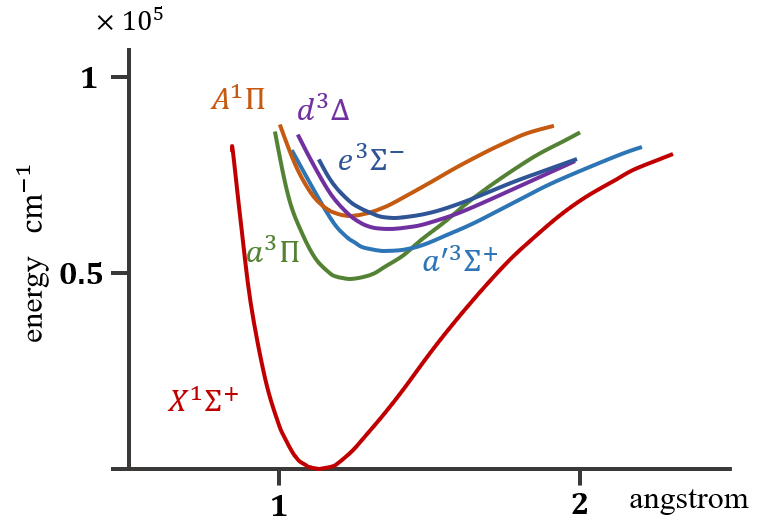
\includegraphics[width=1.0\linewidth]{fig/co_ele_state.png}
% 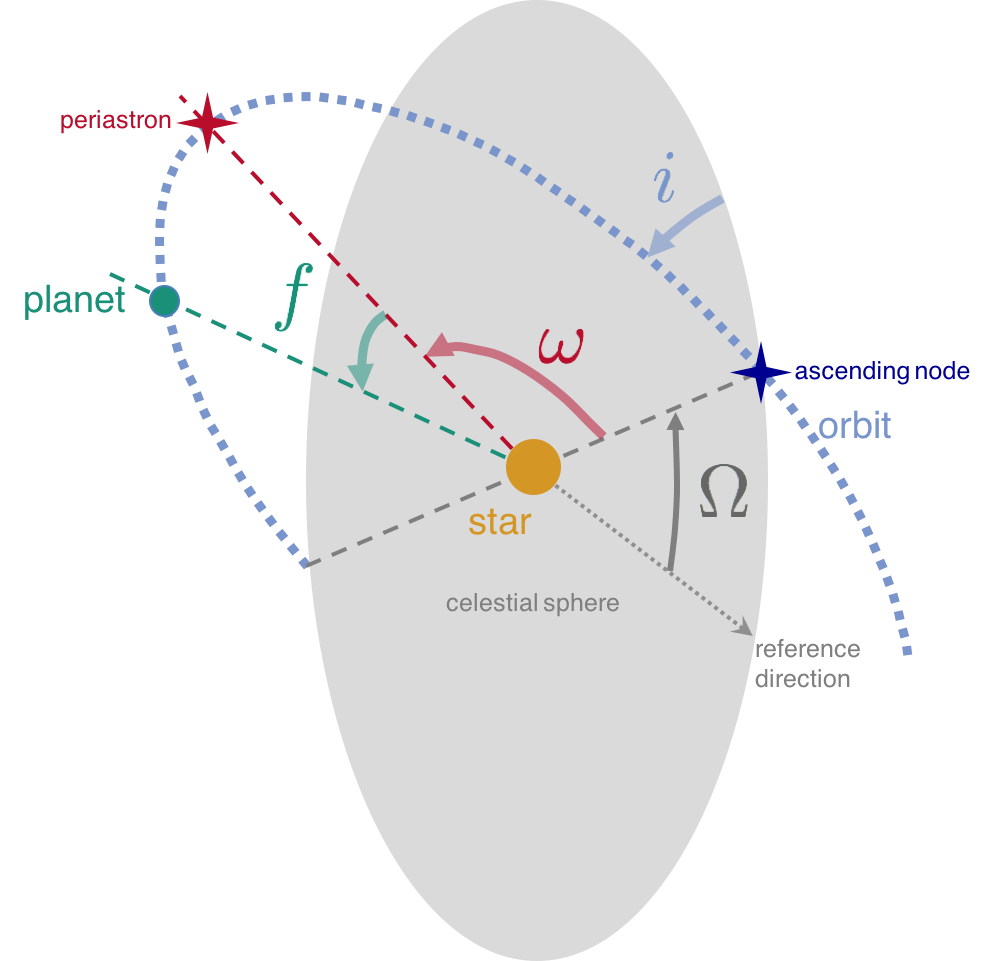
\includegraphics[bb=0 0 474 461,width=1.0\linewidth]{fig/orbele.png}
\end{center}
	\caption{一酸化炭素の電子状態。横軸は核子(炭素-酸素)間距離。}
	\label{fig:co_ele_state}
\end{figure} 

二原子分子では, 電子準位間の遷移, 核子の振動準位間の遷移, 核子の回転準位間の遷移の組み合わせが量子力学的遷移となる. 電子準位については, 核子の運動が電子の運動に比べて極めて遅いため, 核子間の距離$r$を固定して電子の波動方程式を解き, そのエネルギー固有値を求めることができる. 

核子間距離$r$をゆっくり動かしたときに$r$に応じて基底状態の電子のエネルギー固有値が連続的に変化する. 図\ref{fig:co_ele_state}は一酸化炭素の場合の電子のエネルギー固有値(の一部)を核子間距離$r$の関数として書いたものである。系外惑星大気中の分子吸収を考えるときは、通常,電子準位は基底状態(例えばCOなら$\mathrm{X^1} \Sigma^+$)にあると考えてよい\footnote{電子遷移を考える場合もある。}。 このため電子の基底状態のエネルギー固有値を$r$の関数として$V(r)$と表すことができ, 核子 1,2 はポテンシャル$V(r)$中で運動しているとみなすことができる. 

\begin{itembox}{{\it column} -- 電子状態のラベル $\,^\dagger$}
%\tiny
\footnotesize
二原子分子の場合、分子軸($Z$軸)周りの電子の合成軌道角運動量$L_z$が保存することからこの絶対値$\Lambda$を電子状態のラベルとする。$\Lambda$の値に応じた分光学的記号は表\ref{tab:spesymbol}となる。原子の時と同様に分子でもスピン多重度が存在する。スピンを$S
$ ($S=0,1/2,1,3/2,\cdots$)として多重度は$2S+1$である。これを$\Lambda$の左上につけ
\begin{eqnarray}
    \,^{2S+1} \Lambda
\end{eqnarray}
の形で電子状態$n$をラベルする。二原子分子が同じ原子二つからなっている場合(等核二原子分子)、核子の位置の交換に対する操作に対し、波動関数の変化が$\Psi \to \pm \Psi$の二種類の可能性がある。符号を変える場合ungerade(奇数)の頭文字uを、買えない場合gerade(偶数)の頭文字gを用いてこれを右下につける。さらに$\Sigma$状態については分子軸を含む平面上の鏡像反転に関する波動関数の符号の変化の$\pm$を右上につけ、最終的に例えば
\begin{eqnarray}
    \,^{2} \Sigma_u^+
\end{eqnarray}
のような記号となる。表\ref{tab:elebase}に、主な二原子分子の基底状態を示す。また、同じスピン多重度を持つ電子状態で、上のラベルの左側にエネルギーの低い順からX,B,C,D,$\cdots$(基底状態を含む場合)、また基底状態と異なるスピン多重度に対しは、エネルギーの低い順にb,c,d, $\cdots$を付ける表記もある。例えば、
$X\,^1 \Sigma_g^+$ (基底状態)、$B\,^1 \Sigma_u^+$、$C\,^1 \Sigma_u^+$... $a \,^3 \Sigma$ ...
\end{itembox}


\begin{table}[]
    \centering
    \begin{tabular}{c|cccccc}
    \hline\hline
        L & 0 & 1 & 2 & 3 & $\cdots$  \\
        \hline
          & S & P & D & F & $\cdots$  \\
          縮重度 & 1 & 3 & 5 & 7 & (2L+1) \\
        \hline\hline
        $\Lambda$ & 0 & 1 & 2 & 3 & $\cdots$  \\
        \hline
& $\Sigma$ & $\Pi$ & $\Delta$ & $\Phi$ & $\cdots$ \\
        縮重度 & 1 & 2 & 2 & 2 &  
    \end{tabular}
    \caption{原子を考える場合の電子角運動量$L$、二原子分子を考える場合の分子軸(
    $z$)方向角運動量$L_z$の絶対値$\Lambda$と電子状態の記号の対応表。原子の場合,
    縮重度は$2L+1$となるが、分子の場合、$\Lambda=0$を除き、$L_z = -\Lambda$,$\Lambda$の2種類である。}
    \label{tab:spesymbol}
\end{table}

\begin{table}[]
    \centering
    \begin{tabular}{c|c}
    \hline\hline
    分子 & 基底状態\\
    \hline
        \ce{H2} & $\,^1 \Sigma_g^+$\\
        \ce{N2} & $\,^1 \Sigma_g^+$\\
        \ce{O2} & $\,^3 \Sigma_g^-$\\
        \ce{CO} &  $\,^1 \Sigma$\\
        \ce{CN} &  $\,^2 \Sigma$\\
        \ce{NO} &  $\,^2 \Pi$
    \end{tabular}
    \caption{代表的な二原子分子の電子基底状態}
    \label{tab:elebase}
\end{table}


大気中の一酸化炭素分子(CO)のような, 異なる質量$m_1$, $m_2$を持つ2つの核子と複数の電子から構成される自由に運動する二原子分子のエネルギー準位を考える. 電子が常に基底状態にあるとすると, この系は, 核子1, 2がポテンシャル$V(r)$中で運動しているとみなすことができる. ここで$r$は核子間の距離である. $V(r)$は図\ref{fig:co_ele_state} の基底状態とすると、ある$r=r_e \sim 1.2 \AA$で最小値をとり($V_e$とする), 2つの核子は回転運動および$r=r_e$を平衡距離とした振動運動を行う.  


\begin{figure}[h]
\begin{center}
%  \includegraphics[width=70mm]{fig_left.PNG}
  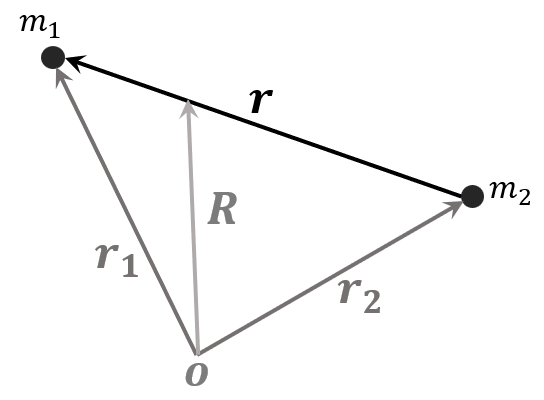
\includegraphics[width=\linewidth]{fig/fig_right.PNG}
\end{center}
\vspace*{-5mm}
\caption{二原子分子の核子の座標. }
\label{fig:phys2_fig1}
\end{figure}


$V(r)$が既知であるとして核子の波動方程式に着目する. 図\ref{fig:phys2_fig1}のように核子の座標をとると, 核子の波動方程式は, 
\begin{align}
  \label{eq:phys2_shro}
&\left( - \frac{\hbar^2}{2 m_1} \nabla_{1}^2  - \frac{\hbar^2}{2 m_2} \nabla_{2}^2 + V(r) \right) \psi(\boldsymbol{r}_1, \boldsymbol{r}_2) \nonumber \\
&= E \psi(\boldsymbol{r}_1, \boldsymbol{r}_2)
\end{align}
と書ける. $\boldsymbol{r}_1$, $\boldsymbol{r}_2$は核子1, 2の位置ベクトルであり, 核子間の距離は$r = |\boldsymbol{r}_1 - \boldsymbol{r}_2|$と表される. また$\nabla_{1}^2$, $\nabla_{2}^2$は核子1, 2のラプラシアン, $\hbar$は, プランク定数を$h$として$\hbar = \dfrac{h}{2 \pi}$, $E$は核子の波動方程式のエネルギー固有値, $\psi(\boldsymbol{r}_1, \boldsymbol{r}_2)$は核子の波動関数である. 式(\ref{eq:phys2_shro})を解くことで核子の振動・回転遷移を考える. 


核子の重心座標
$  \boldsymbol{R} = \displaystyle{\frac{m_1 \boldsymbol{r}_1 + m_2 \boldsymbol{r}_2}{m_1 + m_2} }$
と相対座標
$\boldsymbol{r} = \boldsymbol{r}_1 - \boldsymbol{r}_2$を定義し, $\boldsymbol{r}_1, \boldsymbol{r}_2, \boldsymbol{R}$  換算質量を$\mu = (m_1^{-1} + m_2^{-1})^{-1}$, 総質量を$M = m_1 + m_2$とすると重心座標・相対座標で書かれた波動方程式は
\begin{align}
\label{eq:com_each}
\left( - \frac{\hbar^2}{2 \mu} \nabla_{r}^2  - \frac{\hbar^2}{2 M} \nabla_{R}^2 + V(r) \right) \psi(\boldsymbol{r},\boldsymbol{R}) = E \psi(\boldsymbol{r},\boldsymbol{R})
\end{align}
となる。ここに
重心座標のラプラシアン
$\nabla^2_{R} = \displaystyle{\frac{\partial^2}{\partial X^2} +  \frac{\partial^2}{\partial Y^2} +  \frac{\partial^2}{\partial Z^2}}$
と相対座標のラプラシアン
$\nabla^2_{r} = \displaystyle{\frac{\partial^2}{\partial x^2} +  \frac{\partial^2}{\partial y^2} +  \frac{\partial^2}{\partial z^2}}$
を定義した。

\begin{itembox}{$\clubsuit$式{(\ref{eq:com_each}) $\,^\dagger$}}
%\tiny
\footnotesize
$\boldsymbol{R}, \boldsymbol{r}$の三次元直交座標系の第一成分を
$X, x$, 第二成分を$Y, y$, 第三成分を$Z, z$とする. 
$x$,$X$座標の変換は
\begin{align}
  x &= x_1 - x_2, 
  X = \frac{m_1 x_1 + m_2 x_2}{M} \nonumber 
\end{align}
であるから
\begin{eqnarray}
  \frac{\partial}{\partial x_1} &=& \frac{\partial x}{\partial x_1} \frac{\partial}{\partial x} +
  \frac{\partial X}{\partial x_1} \frac{\partial}{\partial X} =  \frac{\partial}{\partial x} +  \frac{m_1}{M}\frac{\partial}{\partial X}
\end{eqnarray}
より
\begin{align}
    \label{eq:x1}
  \frac{1}{m_1}\frac{\partial^2}{\partial x_1^2} =
  \frac{1}{m_1} \frac{\partial^2}{\partial x^2} + \frac{m_1}{M^2} \frac{\partial^2}{\partial X^2}
   + \frac{2}{M}\frac{\partial}{\partial x}\frac{\partial}{\partial X} 
\end{align}
また
\begin{eqnarray}
  \frac{\partial}{\partial x_2} &=& \frac{\partial x}{\partial x_2} \frac{\partial}{\partial x} +
  \frac{\partial X}{\partial x_2} \frac{\partial}{\partial X} =  - \frac{\partial}{\partial x} +  \frac{m_2}{M}\frac{\partial}{\partial X}
\end{eqnarray}
より
\begin{align}
  \label{eq:x2}
  \frac{1}{m_2}\frac{\partial^2}{\partial x_2^2} =
  \frac{1}{m_2} \frac{\partial^2}{\partial x^2} + \frac{m_2}{M^2} \frac{\partial^2}{\partial X^2}
   - \frac{2}{M}\frac{\partial}{\partial x}\frac{\partial}{\partial X} 
\end{align}

(\ref{eq:x1}, \ref{eq:x2})より
\begin{align}
 \frac{1}{m_1} \frac{\partial^2}{\partial x_1^2} +  \frac{1}{m_2} \frac{\partial^2}{\partial x_2^2} =
  \frac{1}{\mu}\frac{\partial^2}{\partial x^2} + \frac{1}{M}\frac{\partial^2}{\partial X^2}
\end{align}
同様に
\begin{align}
 \frac{1}{m_1} \frac{\partial^2}{\partial y_1^2} +  \frac{1}{m_2} \frac{\partial^2}{\partial y_2^2} &=
  \frac{1}{\mu}\frac{\partial^2}{\partial y^2} + \frac{1}{M}\frac{\partial^2}{\partial Y^2} \\
 \frac{1}{m_1} \frac{\partial^2}{\partial z_1^2} +  \frac{1}{m_2} \frac{\partial^2}{\partial z_2^2} &=
  \frac{1}{\mu}\frac{\partial^2}{\partial z^2} + \frac{1}{M}\frac{\partial^2}{\partial Z^2}
\end{align}
を足して$- \hbar^2/2$をかけると、
\begin{align}
 - \frac{\hbar^2}{2 m_1} \nabla_{1}^2  - \frac{\hbar^2}{2 m_2} \nabla_{2}^2 
= - \frac{\hbar^2}{2 \mu} \nabla_{r}^2  - \frac{\hbar^2}{2 M} \nabla_{R}^2 
\end{align}
となる。
\end{itembox}




波動方程式(\ref{eq:com_each})に対し, 波動関数$\psi(\boldsymbol{R},\boldsymbol{r})$を重心運動の波動関数$\Phi(\boldsymbol{R})$と相対運動の波動関数$\phi(\boldsymbol{r})$および重心運動のエネルギー固有値$E_R$, 相対運動のエネルギー固有値$E_r$を用いて, $\psi(\boldsymbol{R},\boldsymbol{r}) = \Phi(\boldsymbol{R})\phi(\boldsymbol{r})$, $E = E_R + E_r$と変数分離を行う. 重心運動の波動方程式と相対運動の波動方程式をそれぞれ求める。
\begin{align}
  &\Phi(\boldsymbol{R}) \left( - \frac{\hbar^2}{2 \mu} \nabla_{\boldsymbol{r}}^2 \phi(\boldsymbol{r})  + V(r) \phi(\boldsymbol{r}) - E_r \phi(\boldsymbol{r})  \right) \nonumber \\
  &+ \phi(\boldsymbol{r}) \left(  - \frac{\hbar^2}{2 M} \nabla_{\boldsymbol{R}}^2 \Phi(\boldsymbol{R}) - E_R \Phi(\boldsymbol{R}) \right) = 0
\end{align}
と変形できるので重心運動の波動方程式と相対運動の波動方程式としてそれぞれ
\begin{align}
 - \frac{\hbar^2}{2 M} \nabla_{\boldsymbol{R}}^2 \Phi(\boldsymbol{R}) &= E_R \Phi(\boldsymbol{R}) \\
- \frac{\hbar^2}{2 \mu} \nabla_{\boldsymbol{r}}^2 \phi(\boldsymbol{r})  + V(r) \phi(\boldsymbol{r}) &= E_r \phi(\boldsymbol{r}) 
\end{align}
を得る。重心運動の波動方程式は分子自体の運動を表していて、例えば平面波解が対応する。

次に相対運動の波動方程式に対し, 極座標($r, \varphi, \theta$)を用いて
  \begin{eqnarray}
    \label{eq:rotvib}
    \phi(\boldsymbol{r}) = \frac{\phi_r(r)}{r} Y(\varphi, \theta)
  \end{eqnarray}
  のように変数分離を行う. $\phi_r(r)$に対する動径方向$r$の波動方程式は, 回転による遠心力項を$W(r)$として,  有効ポテンシャル$V_\mathrm{eff} (r) = V(r) + W(r)$中を一次元運動する波動方程式に帰着する. $W(r)$を求めよう。

ラプラシアンの極座標表示は、$\nabla^2_{r, \varphi, \theta}$は, 
  \begin{align}
    \nabla^2_{r, \varphi, \theta} &= \frac{1}{r^2} \left( \frac{\partial}{\partial r} r^2 \frac{\partial}{\partial r} + \nabla^2_{\varphi, \theta} \right) \\
          \nabla^2_{\varphi, \theta} &= \frac{1}{\sin{\theta}}\frac{\partial}{\partial \theta}
        \left( \sin{\theta} \frac{\partial}{\partial \theta} \right)
        + \frac{1}{\sin^2 \theta} \frac{\partial^2}{\partial \varphi^2}
\end{align}
で与えられ、球面調和関数$Y_{lm} (\varphi, \theta)$は  
      \begin{eqnarray}
        \nabla^2_{\varphi, \theta} Y_{lm}(\varphi, \theta) + J(J+1) Y_{lm}(\varphi, \theta) = 0 
      \end{eqnarray}
を満たす. ここで$J$は回転量子数$J=0, 1, 2, \cdots$であり, $m$は$|m| \le l$を満たす整数である. 


式(\ref{eq:rotvib})を相対運動の波動方程式に代入し、ラプラシアンを極座標に変換すると
\begin{align}
  &- \frac{\hbar^2}{2 \mu} \left( \frac{1}{r^2} \frac{\partial }{\partial r} r^2 \frac{\partial }{\partial r} + \frac{1}{r^2} \nabla^2_{\varphi,\theta} \right) \frac{\phi_r(r)}{r} Y(\varphi, \theta) \nonumber \\
&+ V(r) \frac{\phi_r(r)}{r} Y(\varphi, \theta) = E_r \frac{\phi_r(r)}{r} Y(\varphi, \theta)
\end{align}
となるが、これを変数分離すると
\begin{align}
\label{eq:separation_vari}
&\frac{r^2}{ \phi_r(r)}\frac{\partial^2}{\partial r^2} \phi_r(r) + \frac{2 \mu r^2}{\hbar^2} (E_r - V(r)) \nonumber \\
&= - \frac{\nabla^2_{\varphi,\theta} Y(\varphi,\theta)}{Y(\varphi,\theta)}
\end{align}
となるから、これを$J(J+1)$と置くことで$Y(\varphi,\theta) = Y_{lm}(\varphi,\theta) $とおくことができる。

\begin{itembox}{$\clubsuit$ 式(\ref{eq:separation_vari}) $\,^\dagger$}
%\tiny
\footnotesize
\begin{align}
  &\frac{\partial}{\partial r} \left(r^2 \frac{\partial}{\partial r} \frac{\phi_r}{r} \right)
  = \frac{\partial}{\partial r} \left( r^2 \frac{r \phi_r^\prime - \phi_r}{r^2}\right) \nonumber \\
  &= \frac{\partial}{\partial r} ( r \phi_r^\prime - \phi_r)
  = \phi_r^\prime + r \phi_r^{\prime\prime} - \phi_r^\prime \nonumber \\ 
  &= r \frac{\partial^2}{\partial r^2} \phi_r(r)
\end{align}
\end{itembox}

すると動径方向の波動方程式は
\begin{align}
&- \frac{\hbar^2}{2 \mu} \frac{\partial^2}{\partial r^2} \phi_r(r) + \left(  V(r) + \frac{\hbar^2 J(J+1)}{2 \mu r^2} \right) \phi_r(r) \nonumber \\
&= E_r \phi_r(r)
\end{align}
が得られ、これは
\begin{align}
V_\mathrm{eff} (r) = V(r) + \frac{\hbar^2 J(J+1)}{2 \mu r^2} 
\end{align}
とした有効ポテンシャル中の一次元の運動とみなすことができる。よって
\begin{align}
  W(r) = \frac{\hbar^2 J(J+1)}{2 \mu r^2} 
\end{align}
となる。 

%      \begin{eqnarray}
%        \left( - \frac{\hbar^2}{2 m} \frac{d^2}{d q^2} + \frac{1}{2} m \omega^2 q^2 \right) f(q) = E^\prime f(q)
%      \end{eqnarray}

\begin{figure*}
    \centering
    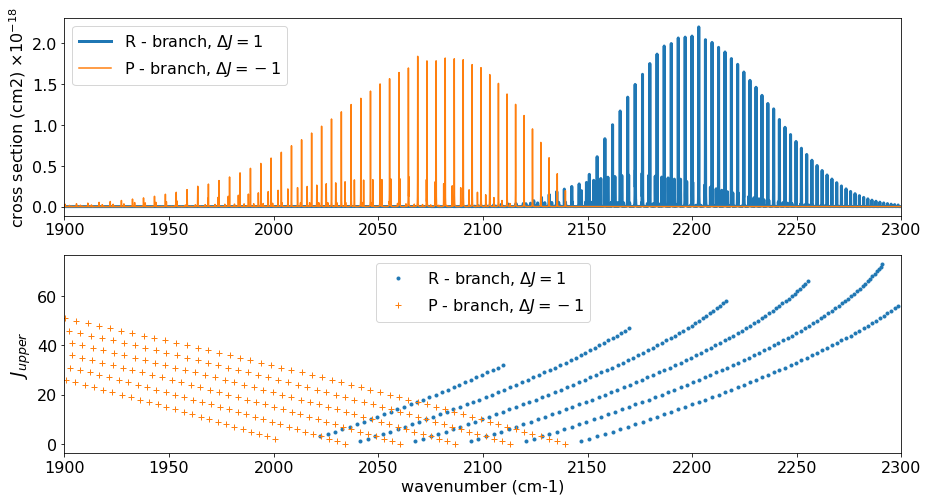
\includegraphics[width=\linewidth]{fig/branch_13_0.png}
    \caption{一酸化炭素の$\Delta \nu=1$遷移におけるR-branch, P-branch断面積。}
    \label{fig:rpbranchco}
\end{figure*}


相対運動のエネルギー固有値$E_r$について, 振動量子数$\nu$と回転量子数$J$の組を用いて, 量子状態を$(\nu,J)$で表記し, 始状態を$(\nu,J) = (\nu_i, J_i)$, 終状態を$(\nu,J) = (\nu_f, J_f)$とする.一酸化炭素のような二原子分子でみられる, $\Delta \nu = \nu_f - \nu_i = 1$, $\Delta J = J_f - J_i = \pm 1$の遷移を考える. 始状態, 終状態の相対運動のエネルギー固有値をそれぞれ$E_r = E_{r, i}$, $E_r = E_{r, f}$と表記し, 遷移エネルギーを$\Delta E = E_{r, f} - E_{r, i}$とする.  

$q=r - r_e$と座標変換する.
\begin{align}
\label{eq:vpotent}
V_\mathrm{eff} (q) &\approx V_e + \frac{\mu}{2} \omega^2 q^2 + \frac{\hbar^2 J(J+1)}{2 \mu (q + r_e)^2} \\
 &\approx V_e + \frac{\mu}{2} \omega^2 q^2 + \frac{\hbar^2 J(J+1)}{2 \mu  r_e^2} 
\end{align}
となるから$\phi_r(x)$に対する波動方程式は
\begin{align}
  &- \frac{\hbar^2}{2 \mu} \frac{\partial^2}{\partial q^2} \phi_r(q) + \frac{\mu}{2} \omega^2 q^2 \phi_r(q) = E^\prime_r \phi_r(q) \\
  &E^\prime = E_r - V_e - \frac{\hbar^2 J(J+1)}{2 \mu r_e^2}
\end{align}
と調和振動子の波動方程式となる。角振動数$\omega$の調和振動子のエネルギー固有値は, $\nu=0, 1, 2, \cdots$を振動量子数として, 
\begin{align}
  E^\prime = \hbar \omega \left( \nu + \frac{1}{2} \right) 
\end{align}
であることから, 元の波動方程式のエネルギー固有値は
\begin{align}
E_r = V_e + \hbar \omega \left( \nu + \frac{1}{2} \right) + \frac{\hbar^2 J(J+1)}{2 \mu r_e^2}
\end{align}
となる。


\begin{align}
E_r(\nu,J) = V_e + \hbar \omega \left( \nu + \frac{1}{2} \right) + \frac{\hbar^2 J(J+1)}{2 \mu r_e^2}
\end{align}
とおく。$E_{r,f} = E(\nu_f, J_f)$, $E_{r,i}=E(\nu_i,J_i)$とおけるため
\begin{align}
  \Delta E &= E_{r,f} - E_{r,i} = E(\nu_f, J_f) - E(\nu_i,J_i) \\
  &= \hbar (\nu_f -\nu_i) + \frac{\hbar^2}{2 \mu r_e^2} [J_f(J_f+1) - J_i(J_i+1)] \\
  &= \hbar \Delta \nu + \frac{\hbar^2}{2 \mu r_e^2} (J_f-J_i)(J_f + J_i + 1) \\
  \label{eq:nl}
  &= \hbar \Delta \nu + \frac{\hbar^2}{2 \mu r_e^2} \Delta J (2 J_i + \Delta J + 1)
\end{align}
となる。


$\Delta \nu = 1$, $\Delta J = 1$を式(\ref{eq:nl})に代入すると
\begin{align}
\label{eq:rbranch}
\Delta E = \hbar \omega + \frac{\hbar^2}{\mu r_e^2} (1 + J_i)
\end{align}
となる。$\Delta \nu = 1$, $\Delta J = -1$を式(\ref{eq:nl})に代入すると
\begin{align}
\label{eq:pbranch}
\Delta E = \hbar \omega - \frac{\hbar^2}{\mu r_e^2} J_i
\end{align}
となる。

これらの帰結は$\hbar \omega$を中心に前後に間隔$\frac{\hbar^2}{\mu r_e^2}$で櫛状に遷移が並ぶということである。図\ref{fig:rpbranchco}はCO ($\Delta \nu =1$)の断面積を示しており、櫛状に並んでいる。波数で右側に伸びる式(\ref{eq:rbranch})の系列をR-branch, 式(\ref{eq:pbranch})をP-branchという。


\section{ラインプロファイルと線強度}

量子力学的効果により分子の遷移エネルギーは離散的であるが、吸収エネルギーは、その離散エネルギーの周りに様々な理由で拡がる。この拡がりをBroadeningと呼ぶ。惑星大気では
\begin{itemize}
    \item 熱運動や乱流によるドップラー拡がり
    \item 不確定性原理による自然拡がり
    \item 分子間のファンデルワールス力に由来する圧力依存の圧力拡がり
\end{itemize}
の三種が重要なBroadeningである。

まず、熱運動によるbroadeningは、原子が熱運動により視線方向に速度$v_x$を持つことでおこるドップラーシフト$\nu = \hat{\nu} ( 1 + v_x/c)$に起因する。$v_x$の分布関数はMaxwell速度分布
\begin{align}
P(v_x) &= \sqrt{\frac{m}{2 \pi k_B T}} \, e^{-\frac{m v_x^2}{2 k_B T}} \\
&= \sqrt{\frac{m}{2 \pi k_B T}} \, e^{-\frac{m c^2 (\nu - \hat{\nu})^2}{2 k_B T \hat{\nu}^2}} 
\label{eq:dopplerveldist}
\end{align}
に比例してラインが広がること。HWHM (half width at half maximum)、
\begin{eqnarray}
\gamma_D = \hat{\nu} \sqrt{\frac{2 (\log{2}) k_B T}{m c^2}}
\label{eq:dopplergamma}
\end{eqnarray}
を用いて、ドップラー拡がりのline profileは
\begin{eqnarray}
g_D(\nu; \hat{\nu}; \gamma_D) = \sqrt{\frac{\log{2}}{\pi}} \frac{1}{\gamma_D} e^{ - \log{2} \left( \frac{\nu - \hat{\nu}}{\gamma_D}\right)^2}
\label{eq:dopplerprofile}
\end{eqnarray}
となる。すなわちドップラー拡がりはガウス分布に従う。乱流(ミクロ乱流)による速度分散も同様にガウス分布で近似されるが、現在のところあまり考慮されていない。

一方、圧力広がりと自然拡がりは共にLorentz profile、
\begin{eqnarray}
g_L(\nu; \hat{\nu}; \gamma_L) &=& \frac{\gamma_L/\pi}{(\nu - \hat{\nu})^2  + \gamma_L^2}
\label{eq:lorentzprofile}
\end{eqnarray}
で表される。ここにHWHMを$\gamma_L$としている。

惑星大気では特に圧力拡がり (van der Waals Broadening)が重要である。地球大気の場合、$p_0=$1 atmosphere、$T_0=$296 Kでの$\gamma_{L, \mathrm{W}}$を、air-broadening coefficient $\gamma_{L, \mathrm{W}}^{\mathrm{air}}$ といい、これを用いて、
\begin{eqnarray}
\gamma_{L, \mathrm{W}}(p,T) = \gamma_{L, \mathrm{W}}^{\mathrm{air}} \frac{p}{p_0} \left( \frac{T_0}{T} \right)^\alpha
\label{eq:airtogen}
\end{eqnarray}
のように圧力拡がりを計算することが多い。ここに$\alpha$は温度依存項のべき(temperature exponent)で代表的には0.5程度であるがさまざまである。圧力拡がりは周囲の分子からのファンデルワールス力に起因するので、背景大気の種類によって異なる。特に系外惑星大気では水素分子・ヘリウム大気であることが多く、地球の大気下での値と異なることに注意が必要である。


自然拡がりは、不確定性原理からくるラインの広がりである。アインシュタイン$A$係数を用いて
\begin{eqnarray}
\gamma_{L, \mathrm{n}} = \frac{A}{4 \pi c} = \frac{0.222}{4 \pi c} \left( \frac{\nu}{\mathrm{cm^{-1}}} \right)^2 \mathrm{[cm^{-1}]}
\end{eqnarray}
となる。これは電子が励起状態に滞在する確率が$e^{-A t}$のようになることと不確定性関係に由来している。圧力拡がりに対し、自然拡がりは低圧下で寄与が大きくなる。

上記のDoppler profileとLorentz profileの両方が効く場合、両者をconvolutionしたものがline profileとなる。これをVoigt profile\index{Voigt profile@Voigt profile}と呼ぶ。
\begin{align}
&g_V(\nu;\hat{\nu}) = ( g_L \ast g_D )(\nu; \hat{\nu}) \nonumber \\ &= \int_{-\infty}^\infty d \nu^\prime g_L(\nu - \nu^\prime;\hat{\nu};\gamma_L) g_D(\nu^\prime - \hat{\nu};\hat{\nu};\gamma_D) 
\label{eq:voigt}
\end{align}
となる。圧力拡がりと自然拡がりの両方が寄与する場合は、$\gamma_L$として
\begin{eqnarray}
\label{eq:sumgamma}
\gamma_L &=& \gamma_{L, \mathrm{W}} + \gamma_{L, \mathrm{n}}
\end{eqnarray}
を用いれば良い。これはLorentian同士の畳み込みが
\begin{align}
&g_L(\nu;\hat{\nu},\gamma_{L,\mathrm{W}}) \ast g_L(\nu;\hat{\nu},\gamma_{L,\mathrm{n}}) \nonumber \\ &= \int_\infty^\infty d \nu^\prime g_L(\nu - \nu^\prime;\hat{\nu};\gamma_{L,\mathrm{W}}) g_L(\nu^\prime - \hat{\nu};\hat{\nu};\gamma_{L,\mathrm{n}}) \\
&= \frac{(\gamma_{L,\mathrm{W}}+\gamma_{L,\mathrm{n}})/\pi}{(\nu - \hat{\nu})^2  + (\gamma_{L,\mathrm{W}}+\gamma_{L,\mathrm{n}})^2} \nonumber \\
&= g_L(\nu;\hat{\nu},\gamma_{L,\mathrm{W}}+\gamma_{L,\mathrm{n}})
\label{eq:voigt2}
\end{align}
となるからである。またLorentianのテイルは無限に続くわけではなくある程度、線中心から離れると($O(10^2) \mathrm{cm^{-1}}$)急激にカットオフが効くとされている。このSub--Lorentian効果についてはわかってないことが多いが、広い波数域で計算する際には注意が必要である。


またラインプロファイルは
\begin{align}
    \int d \nu g(\nu) = 1 
\end{align}
に規格化されているため$g(\nu)$の次元は$\mathrm{cm}$である。

光子が分子によって吸収される過程を考える。分子分光では、エネルギーに対応する量を$hc$で割って、波数で表すことが一般的である。ここでもこの表記法に習おう。また、光の吸収を考えるので、終状態は始状態より高いエネルギーである。そこで終状態を$\mathrm{up}$ (upper state)は初期状態を$\mathrm{low}$ (lower state)のラベルに書き換える。
例えば、$E_\mathrm{low} = E_{\nu_i, J_i}/hc$, $E_\mathrm{up} = E_{\nu_f, J_f}/hc$である。

光の吸収に関して各ラインの強度は、下の順位$E_\mathrm{low} $からの誘導吸収により生じるため、その状態の数に比例して強くなる。ただし、光が入射することで生じる誘導放射により実効的な吸収が減るため、この補正も必要である。

$E_\mathrm{low}$の状態の数は、局所熱力学平衡にあると
\begin{align}
\label{eq:lte}
    \frac{n_\mathrm{low}}{n} &= \frac{\mathsf{g}_\mathrm{low}}{Q(T)} \exp{\left(- \frac{h c E_\mathrm{low}}{k_B T} \right)}
\end{align}
となる。ここに$\mathsf{g}_\mathrm{low}$は縮退度、$n$は全状態数、$Q(T)$は分配関数である。また誘導放射による補正は$(1- e^{-h c \hat{\nu}/k_B T})$である。ここに$\hat{\nu}$は吸収波数、つまりupper/lower statesの差の$\hat{\nu} = E_\mathrm{up} - E_\mathrm{low}$のことである\footnote{この量を$E$を使って表さないのは、分光的に問題となる実際に吸収中心である波数であるからであろう。}。

係数も含めると線強度とはラインプロファイル$g(\nu)$を用いて断面積が
\begin{align}
    \sigma^2 (\nu) = S(T) g(\nu)
\end{align}
となる量である。つまり$S(T)$の次元は$\mathrm{cm}$である。

\begin{align}
\label{eq:STexomol}
S(T) &=\displaystyle{ \frac{\mathsf{g}_\mathrm{up}}{Q(T)} \frac{ A}{8 \pi c \hat{\nu}^2} e^{-  c_2 E_\mathrm{low}/T} {\left(1- e^{-c_2 \tilde{\nu}/T}\right)}},
\end{align}
となる。ただし$c_2 \equiv hc/k_B = 1.4387773 \, \mathrm{cm K}$である。$A$はアインシュタインA係数である。

\begin{itembox}{$\clubsuit$ 式(\ref{eq:STexomol}) $\,^\dagger$}
%\tiny
\footnotesize
実効的に起きる吸収は、誘導吸収($B_{lu}$)から誘導放射($B_{ul}$)を差し引いたものである。つまり
\begin{align}
    S(T) &= \frac{h c \hat{\nu}}{c} \left( \frac{n_\mathrm{low}}{n} B_{lu} - \frac{n_\mathrm{up}}{n} B_{ul} \right) 
\end{align}
が実効的におこる吸収である。局所熱力学平衡の場合、
\begin{align}
     \frac{n_\mathrm{up}}{n_\mathrm{low}} &= \frac{\mathsf{g}_\mathrm{up}}{\mathsf{g}_\mathrm{low}} \exp{\left(- \frac{h c (E_\mathrm{up} - E_\mathrm{low})}{k_B T} \right)} \\
     &= \frac{\mathsf{g}_\mathrm{up}}{\mathsf{g}_\mathrm{low}} e^{-hc \hat{\nu}/k_B T}
\end{align}
である。また詳細つり合いから
\begin{align}
    \mathsf{g}_\mathrm{low} B_{lu} &= \mathsf{g}_\mathrm{up} B_{ul} \\
    A &= 2 \pi h c \hat{\nu}^3 B_{ul}
\end{align}
となるが、これらを用いると
\begin{align}
    S(T) &= \frac{h \hat{\nu}}{4 \pi} \frac{n_\mathrm{low}}{n} B_{lu} (1 -  e^{-hc \hat{\nu}/k_B T}) \\
    &= \frac{\mathsf{g}_\mathrm{up}}{Q(T)} \frac{ A}{8 \pi c \hat{\nu}^2} e^{- h c E_\mathrm{low}/k_B T} {\left(1- e^{- h c \tilde{\nu}/k_B T}\right)}
\end{align}
が得られる。途中で式(\ref{eq:lte})を用いた。
\end{itembox}



\section{様々な分子の振動回転遷移$^\ddagger$}
\subsection*{メタン}
%https://doi.org/10.1016/j.jqsrt.2024.108897

\begin{figure}
    \centering
    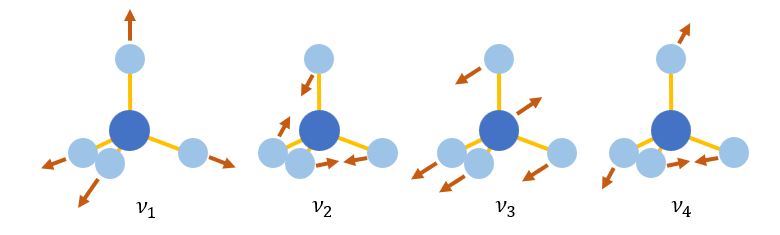
\includegraphics[width=\linewidth]{fig/methanevib.png}
    \caption{メタンの4種振動モード}
    \label{fig:ch4vib}
\end{figure}

図\ref{fig:ch4vib}に示すように、メタンの振動モードは4種類$\nu_1, \nu_2, \nu_3, \nu_4$があり、そのうち赤外活性つまり赤外域での光子吸収があるのは$\nu_3$と$\nu_4$である。これらは基本バンドとして、それぞれ3.25--3.45 $\mu$m, 7.5--8.0$\mu$mに強い吸収を持つ。またそれ以外の場所にもPolyad構造による吸収(ホットバンド)が多数存在する。Polyad構造は
$\nu_1 \simeq \nu_3 \simeq 2 \nu_2 \simeq 2 \nu_4 \simeq 3000\mathrm{cm}^{-1}$ となることに起因する構造であり、polyad数
\begin{align}
\mathrm{P} =  2 (\nu_1 + \nu_3) + \nu_2 + \nu_4 
\end{align}
で特徴づけられる。それぞれ
Monad (P=0),
Dyad (P=1),
Pentad (P=2),
Octad (P=3),
Tetradecad (P=4),
Icosad (P=5),
Triacontad (P=6),
Tetracontad (P=7),
の名前がついていて、エネルギーは大まかに$1500 P \mathrm{cm}^-1$程度となる。例えば褐色矮星のHバンドに見られる1.6$\mu$m付近のメタン吸収はP=4のTetradecadに対応することが分かる\cite{2024JQSRT.31608897K}。\\


\subsection*{二原子分子のバンドヘッド}

調和振動子近似ではポテンシャルが核子間距離の二次の関数であるとし、式(\ref{eq:vpotent})の遠心力項が核子間の距離の関数であることを無視していた。実際、この近似は、図\ref{fig:rpbranchco}のように、一酸化炭素の$\Delta \nu=1$遷移をよく説明できる。
しかし、振動遷移$\Delta \nu$が大きくなってきて核子間距離の、これらの近似が破れてきて、バンドヘッドという構造が表れる。ポテンシャルは
\begin{align}
\label{eq:vpotent_}
V_\mathrm{eff} (q) &\approx V_e + \frac{\mu}{2} \omega^2 q^2 + \frac{\hbar^2 J(J+1)}{2 \mu r_e^2 [1 + (q/r_e)^2]} \\
&\approx \frac{\hbar^2 J (J+1)}{2 \mu r_e^2} \left[1 - 2 \frac{q}{r_e} + 3 \left(\frac{q}{r_e} \right)^2 \cdots + \right]
\end{align}
と表されるが、この右辺第三項の$q/r_e$が大きくなると、遠心力が弱くなる効果が存在する。また、ポテンシャル自身も図\ref{fig:co_ele_state}の基底状態で示すように平衡位置から離れると二次近似から逸脱してくる。これらの効果を摂動論として計算すると、(省略するが)この計算は$X=(\nu + 1/2)$と$Y=J(J+1)$の二次式の形となる。

クロスターム($XY$)以外の二次の項は無視した形式を記すと
\begin{align}
    \label{eq:nonharmo_cen}
    E_r (\nu, J) &= V_e + \hbar \omega \left( \nu + \frac{1}{2} \right) + B_\nu J (J+1)  \\
    \label{eq:nonharmo_cen_x}
    B_\nu &= \frac{\hbar^2}{2 \mu r_e^2} - \alpha_0  \left( \nu + \frac{1}{2} \right) 
\end{align}
となる。これは振動が大きくなると、非調和ポテンシャルでは平均的な核間距離が延びることで、回転定数$B_\nu$が小さくなるという描像である。

式(\ref{eq:nonharmo_cen_x})を用いて評価すると $B_{\nu+1} - B_\nu = - \alpha_0$であるので、R, P-branchはそれぞれ
\begin{align}
\label{eq:u_fort_R}
    h \hat{\nu}^R_{\mathrm{line}} (J_u) &= h \nu_\nu  + 2 B J_u - \alpha_0 J_u^2  \\
\label{eq:u_fort_P}
    h \hat{\nu}^P_{\mathrm{line}} (J_u) &=  h \nu_\nu - 2 B (J_u + 1) - \alpha_0 (J_u + 1)^2 \\
    B &\equiv B_0 + \frac{1}{2} \alpha_0
\end{align}
となり二次関数となる。

$\alpha_0 > 0$とすると、R-branchの変曲点は$J_u = B/\alpha_0 > 0$となるので\footnote{一方、P-branchの変曲点は$- B/\alpha_0 < 0$であるので、$J_l = J_u+1 > 0$の領域に変曲点は存在しない。ただしこれは$\alpha_0>0$の場合である。}、振動回転遷移の波数最大値(波長最小値)が存在し、このエネルギー付近に多数の遷移が集まることがわかる(図\ref{fig:rpbranch}の下パネル)。これをband headと呼ぶ。図\ref{fig:rpbranch}に2.3ミクロン付近のCOのband headの例を示した。今回横軸は波長であることに注意が必要である。band head付近の準位が多い温度では、band head付近の吸収が強くなる(図\ref{fig:rpbranch}の上パネル)。

\begin{figure*}
    \centering
    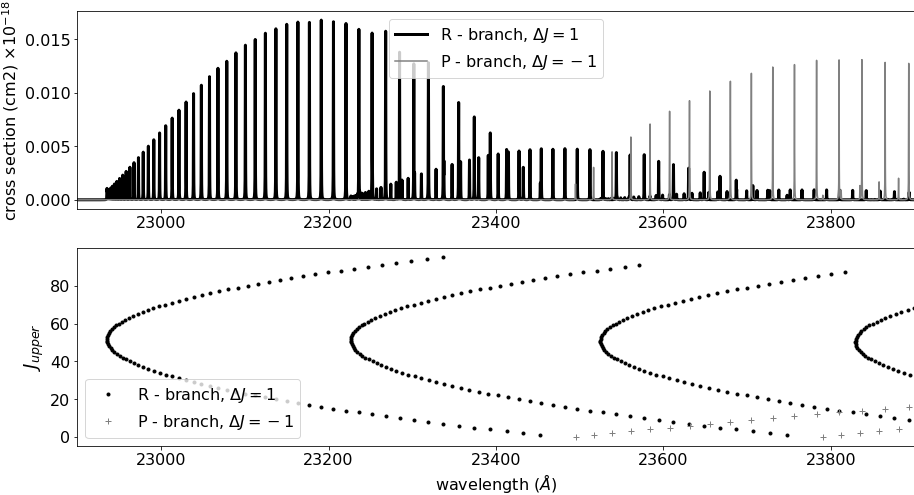
\includegraphics[width=0.9\linewidth]{fig/bandhead.png}
    \caption{CO 2.3ミクロン帯 ($X\,^1 \Sigma^+$, $\Delta \nu = 2$)のband headの例。$J_{upper}$のエネルギー増加が減少に転じる点に多数の遷移が集まりband headが生じる。}
    \label{fig:rpbranch}
\end{figure*}



また式(\ref{eq:u_fort_R})と(\ref{eq:u_fort_P})を一つの式にまとめて、
\begin{align}
    h \hat{\nu}_{\mathrm{line}} (\mathcal{J}) &=  h \nu_\nu - 2 B \mathcal{J} - \alpha_0 \mathcal{J}^2 
\end{align}
ただし、
\begin{align}
    \mathcal{J} = \left\{
\begin{array}{ll}
J_u & (\mathcal{J} > 0)\\
- J_l & (\mathcal{J} < 0)
\end{array}
\right.
\end{align}
としたものを、縦軸$\mathcal{J}$、横軸ライン中心波数で書いたものを
R. Fortratにちなんでフォルトラ図という(図\ref{fig:fortrat})。振動エネルギーの差にあたる$\mathcal{J}=0$の値$\nu_\nu$にはラインがない。これをバンド原点(Band origin)と呼ぶ。

\begin{figure*}
    \centering
    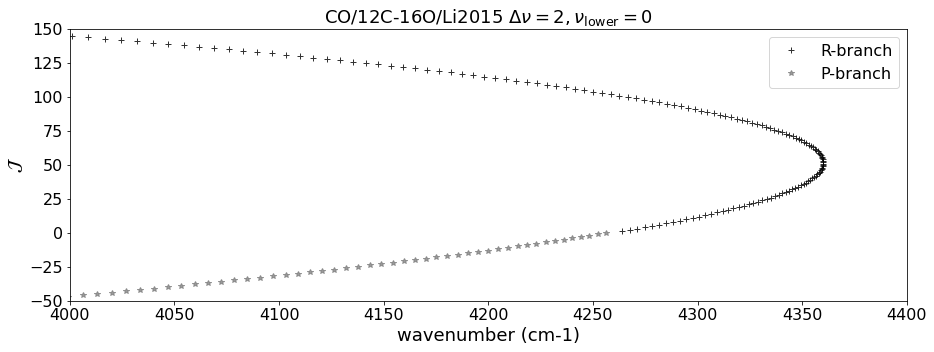
\includegraphics[width=0.9\linewidth]{fig/fortrat.png}
    \caption{COのフォルトラ図。$\Delta \nu=2$, $\nu_\mathrm{lower}=0$の場合を示している。}
    % exojax/documents/tutorials/Fortrat.ipynb
    \label{fig:fortrat}
\end{figure*}

\section{重力と惑星大気}
惑星大気は、惑星の重力により惑星表面に束縛されている。すなわち重力が大気構造の大まかな構造をあたえる。大気構造に以下の仮定をおいて簡単化し、大気構造と重力の関係を見る。
\begin{itemize}
    \item 大気層は薄く平衡平板で近似できる
    \item 大気は等温
    \item 大気は理想気体としてふるまう
    \item 大気の鉛直方向の運動はなく、重力と圧力が釣り合っている
\end{itemize}
ここから、大気の重要な長さスケールであるスケールハイトが導入される。

\subsection*{理想気体の状態方程式 \label{ss:idealgass}}
単一成分の理想気体の状態方程式は、圧力$P$、温度$T$、気体数密度$n [\mathrm{cm^{-3}}]$を用いて
\begin{eqnarray}
\label{eq:ideal}
P = n k_B T
\end{eqnarray}
となる。アボガドロ数$N_A=6.0221367 \times 10^{23}$を利用して
\begin{eqnarray}
\label{eq:idealRastmol}
P &=& R^\prime n^\prime T 
\end{eqnarray}
とも書ける。ここに$R^\prime = N_A k_B = 8.3144598 \times 10^7 [\mathrm{erg/K/mol}]$ はuniversal gas constant\index{universal gas constant@universal gas constant}である。ここに$n^\prime$はモル数密度$[\mathrm{mol \, cm^{-3}}]$である。式(\ref{eq:ideal})を気体密度$\rho = \mu m_H n \,\,[\mathrm{g \, cm^{-3}}]$ ($\mu$は分子量、$m_H$はproton mass)であらわすと、
\begin{eqnarray}
\label{eq:idealRast}
P &=& \frac{k_B}{\mu m_H} \rho T \\
\end{eqnarray}
となる。 specific gas constant $R \,\,[\mathrm{erg/g/K}]$を用いてかくと
\begin{eqnarray}
\label{eq:idealR}
P &=& R \rho T \\
R &\equiv& \frac{k_B}{\mu m_H}
\end{eqnarray}
となる。以上のように$R^\prime$を用いてモル数密度で考えているのか、$k_B$もしくは$R$を用いて、通常の密度・数密度で考えているのか区別する必要がある。本稿では宇宙分野の表記との一貫性を保つため、原則は通常の密度・数密度で考える。しかし、気象学の分野では数密度のmol表記が一般的であり、比較の際や文献値を使用する際には表記の違いに注意が必要である。



\subsection*{等温・静水圧平衡 \label{ss:atmscal}}

惑星の地表においた薄い大気層においては重力加速度
\begin{eqnarray}
g = - \frac{d \phi}{d r} = \frac{G M_p}{r^2}
\end{eqnarray}
($\phi=G M_p/r$は重力ポテンシャル)を$r$に寄らず一定と近似することができる。この条件下で静水圧平衡
\begin{eqnarray}
\label{eq:pressureeq}
\frac{d P(r)}{d r}  = \rho \frac{d \phi}{d r} =  - \rho g 
\end{eqnarray}
に、状態方程式(\ref{eq:idealRast})を用いると微分方程式
\begin{eqnarray}
\frac{d P}{d r} = - \frac{P}{H} 
\end{eqnarray}
の形となり解は
\begin{eqnarray}
\label{eq:pusi}
P(r) = P_0 \exp{\left( -\frac{r-r_0}{H} \right) } \equiv P_\mathrm{thin} (r)
\end{eqnarray}
となる。$r_0$での圧力を$P_0$として境界条件とした。ここに
\begin{align}
  \label{eq:scale_height}
H &\equiv \frac{k_B T}{\mu m_H g} \\
&\approx 8.4 \,\, \mathrm{km} \left( \frac{T}{300 \,\, \mathrm{K}} \right)  \left( \frac{\mu}{30} \right)^{-1} \left( \frac{g}{980 \,\, \mathrm{cm/s^2}} \right)^{-1}
\end{align}
は(圧力)スケールハイトとよばれる。つまり、熱エネルギーと重力の比で大気の典型的な高さが決まる単純な描像が得られる。長さの次元を持つ大気の高さには熱エネルギー、すなわち温度情報が必要であることがわかる。

式(\ref{eq:scale_height})から、例えば、温度の高い惑星のほうが大気の高さがあるため観測しやすいことなどがわかる。岩石惑星の場合、密度がほとんど半径によらないため、$H$は半径に反比例する。すなわち半径が二倍地球半径のスーパー・アースは、半径は二倍になるが大気の厚さは半分になるため、透過光分光による大気キャラクタリゼーションの難しさはあまり変わらない。また、式(\ref{eq:pusi})から、ある$r > r_0$の$r_0$からの高さを圧力から求めるには、
\begin{eqnarray}
\Delta r = (r - r_0) = H \log{\left(\frac{P_0}{P(r)}\right)}  
\end{eqnarray}
となる。

また大気中で等温とみなせる薄い一層を考え、そのレイヤーの高さ幅を$d z (> 0)$、圧力単位での幅を$d P (>0)$とすると、式(\ref{eq:scale_height})から
\begin{eqnarray}
\label{eq:conversion_z_P}
\frac{d P}{P} = \frac{d z}{H} 
\end{eqnarray}
と書ける。このようにスケールハイトで規格化された高さの変化が圧力の相対変化と一致する。改めて書くほどではないが、式(\ref{eq:pressureeq})から高さ座標と圧力座標の変換は
\begin{eqnarray}
\label{eq:pressureeq_}
d z = \frac{d P}{\rho g}
\end{eqnarray}
である。

\section{大気と分子存在量}

前節では等温であるとしたが、一般には大気は等温ではない。大気の高さを長さの次元で考えるためには、上で見たように温度情報が必要であるが、これが等温でない場合、複雑になってしまう。そこで大気の高さを長さの次元ではなく、圧力で代用する方法が良く用いられる。この場合、温度の鉛直構造は縦軸圧力・横軸温度であらわされるが、圧力軸は鉛直方向を示すためが逆転させることが多い。


また大気からの放射や透過・反射を考える場合、光学的厚さと圧力を変換する必要がある。式(\ref{eq:pressureeq})より、
\begin{eqnarray}
\label{eq:drdp}
d r = - \frac{d P}{\rho g} 
\end{eqnarray}
であるから、断面積を$\sigma$とした光学的厚さの微分形は
\begin{eqnarray}
d \tau = - n \sigma d r = \frac{\sigma}{\mu m_H g} d P  
\end{eqnarray}
と表される。ただし符号は$\tau$をどちらから測るかに依存する。今は、$r \to \infty$を$\tau \to 0$と定義している。この表記でも陽に温度にはよらないことに注意。ただし、一般的に断面積は温度・圧力に依存する。またガス組成の鉛直分布依存に対応して平均分子量も厳密には圧力に依存する、すなわち
\begin{eqnarray}
\label{eq:dtaudP}
d \tau = \frac{\sigma(T,P)}{\mu (P) m_H g} d P  
\end{eqnarray}
である。ただし、ここでは薄い大気を考えているので$g$は圧力によらないことに注意。\\

\subsection*{多成分系}

大気が多成分系からなる場合はどうだろうか? $m_H$をプロトン質量とすると、第$i$成分の分圧は
\begin{eqnarray}
\label{eq:idealRpa}
P_i &=& k_B n_i T = R \rho_i T 
\end{eqnarray}
である。今、密度と数密度の関係は
\begin{eqnarray}
\label{eq:rhon}
\rho &=& \sum_{i=1}^N \rho_i = m_H \sum_{i=1}^N \mu_i n_i  \\
&=& m_H \left( \sum_{i=1}^N \mu_i \frac{ n_i}{n} \right) n = m_H \, \mu \,n \\
\label{eq:moc}
\mu &\equiv& \sum_{i=1}^N \xi_i \mu_i 
\end{eqnarray}
と表せる。ここに総数密度$n= \sum_{i=1}^N n_i$を定義した。また$\mu$は平均分子量であり、$\xi_i = n_i/n$は体積混合率(Volume Mixing Ratio; VMR) 
\index{たいせきこんごうひ@体積混合比}
と呼ばれる量である。体積混合比は分圧と
\begin{eqnarray}
\label{eq:partial_pressure}
    P_i = \xi_i P
\end{eqnarray}
の関係がある\footnote{体積混合比は、ガスの気体分子全体の数に対する分子Aの数の割合であり、なぜこの量を体積混合比と呼び、数混合比と呼ばないのかは不明である。}。また式(\ref{eq:moc})の両辺を$\mu$で割ることにより
\begin{align}
    1 &=  \sum_{i=1}^N X_i \\
    \label{eq:mmr_vmr}
    X_i &=  \frac{\mu_i}{\mu} \xi_i \\
    & = \frac{\rho_i}{\rho}
\end{align}
となる。$X_i$は、全ガスに占める分子$i$の質量の割合を示し、質量混合比(Mass Mixing Ratio; MMR)\index{しつりょうこんごうひ@質量混合比}と呼ばれる。

密度表記の状態方程式は平均分子量$\mu$を用いて
\begin{eqnarray}
\label{eq:idealRpat}
P &=&  \sum_{i=1}^N P_i = k_B n T = R \rho T  \\
R &\equiv& \frac{k_B}{\mu m_H}
\end{eqnarray}
と一成分系のように扱える。\\


\subsection*{分子存在量推定と基本縮退}

分子多成分系の場合、第$i$成分のopacityは、式(\ref{eq:partial_pressure})、式(\ref{eq:mmr_vmr})より
\begin{align}
d \tau_i &= - n_i \sigma_i d r = \frac{\sigma_i}{\mu m_H g} d P_i \\
&= \frac{\xi_i \sigma_i}{\mu m_H g} d P  \\
\label{eq:MMR_dP_dtau}
&= \frac{X_i \sigma_i}{\mu_i m_H g} d P 
\end{align}
となる。

ここで式(\ref{eq:MMR_dP_dtau})をよく見ると、$\sigma_i, \mu_i, m_H$は大気とは無関係に物理化学的に決まる量であるが、$X_i$と$g$は系に固有の量であり、観測の観点からは推定量である。しかし$d \tau_i$は$X_i/g$にのみ依存しているため、これを同時に決めることはできない。分子だけでオパシティが決まる場合の総光学的厚さは、線形和
\begin{align}
\label{eq:mol}
    d \tau = - \sum_{i=1}^N n_i \sigma_i dr = \sum_{i=1}^N d \tau_i
\end{align}
となっていることから、結局、スペクトルから推定できるのは、分子存在量ではなく、質量混合比を重力で割った$X_i/g$のみである。これを我々は{\bf 基本縮退}と呼んでいる。


トランジット系の場合、RVとトランジット半径から$g$が決まるため、基本縮退は解けるの問題はない。直接撮像惑星や褐色矮星の直接分光のような放射光のみの場合、photosphereが分子吸収しか見えない場合、基本縮退は解けない。しかし水素分子等による連続吸収が見える場合は基本縮退が解けるようになる\cite{2025ApJ...988...53K}。

\section{雲}

系外惑星・褐色矮星大気の推定では、雲のモデルが必要である観測スペクトルも多い。雲のモデルは、実際の解析には簡単に灰色の色依存性のない連続オパシティとして扱われることも多い。しかしここでは雲の微物理に踏み込んだモデルを紹介する\footnote{雲の微物理の深い議論はPruppacher and Klett\cite{pruppacher2010microstructure}を参照}。特に系外惑星の雲モデルのseminal paperであるAckerman and Marley\cite{ackerman2001precipitating}に雲モデルを紹介する。 雲は、大気中に存在する気体から固体もしくは液体に想定することで発生する。地球大気の雲は主にH2Oによるものであるが、液体の雲(水雲)と固体の雲(氷雲)がある。 表\ref{tab:input2}に、系外惑星や褐色矮星で考える主な雲の構成成分を示した。

\begin{table}[!tbh]
\begin{center}
\caption{典型的な雲粒子の構成成分とその物質密度。\label{tab:input2}}
\begin{tabular}{lcc}
  \hline\hline
  通称&分子式&物質密度$\delta_\cond (\mathrm{g/cm^{3}}$) \\
  \hline
water&H2O& 1 \\
&NH3& \\
Fe (固体) &Fe&7.875\\
ferrous oxide&FeO&5.987\\
phosphate &H3PO4& \\
&KCl&\\
&Na2S&\\
&TiO&\\
&SiC&\\
&VO&\\
hematite     &Fe2O3&5.275\\
magnetite    &Fe3O4&5.200\\
fayalite     &FeSiO4&4.393\\
corundum     &Al2O3&3.987\\
quartz       &SiO2&2.648\\
rutile       &TiO2&4.245\\
enstatite    &MgSiO3&3.194\\
forstelite   &Mg2SiO4&3.214\\
\end{tabular}
\end{center}
\end{table}

\subsection*{雲粒子の終端速度}\label{ss:termv}

雲粒子が落下し、空気抵抗力$F_d$+浮力$F_a$と重力が釣り合った定常の速度になったとする。この速度を終端速度(terminal velocity)という。釣り合いの式は
\begin{align}
F_d + F_a = m (r) g 
\end{align}
である。$m(r)$は雲粒子の質量、$g$は重力定数である。雲粒子の物質密度を$\delta_\cond$、大気の密度を$\rho$とする。
\begin{align}
m(r) &= \frac{4 \pi}{3} r^3 \delta_\cond \\
F_a &= \frac{4 \pi}{3} r^3 \rho g 
\end{align}
なので
\begin{align}
\label{eq:Fd}
F_d &= \frac{4 \pi}{3} r^3 (\delta_\cond - \rho) g \\
&\approx  \frac{4 \pi}{3} r^3 \delta_\cond g 
\end{align}
となる。最後の近似は、通常$\delta_\cond \gg \rho$なので浮力を無視している場合である。

抵抗力$F_d$は、一般的に終端速度$v_f$と抵抗係数$C_d$を用いて
\begin{align}
F_d = C_d \frac{\rho v_f^2}{2} (\pi r^2)  
\end{align}
の形にかける(証明略)。ここで無次元数レイノルズ数
\begin{align}
\label{eq:Reynolds}
N_{re} = \frac{2 \rho v_f r}{\eta}
\end{align}
を用いて、
\begin{align}
F_d = 6 \pi \eta r v_f \left( \frac{C_d N_{re}}{24} \right)
\end{align}
の形に書き直せる。式(\ref{eq:Fd})と合わせると
\begin{align}
\label{eq:gcloud}
v_f(r) = \frac{2}{9 \eta}  g r^2 (\delta_\cond - \rho) \left( \frac{C_d N_{re}}{24} \right)^{-1}
\end{align}
となる。ただし$\eta$はdynamic viscosity.


ここで$C_d$はレイノルズ数によってことなる。$N_{re} \ll 1$の場合、
\begin{align}
C_d = \frac{24}{N_{re}}
\end{align}
のStokes flowとなる。粒子サイズが小さい場合、粒子表面での滑りが生じ、そのための補正、Cunningham補正係数$(1+1.26 N_{Kn})$、$N_{Kn}=k_B T/\sqrt{2 \pi r^2 P L}$はKnudsen数の補正をいれる。
結果の終端速度は
\begin{align}
\label{eq:sfcloud}
v_f^{sf}(r) = \frac{2}{9 \eta} g r^2 (\delta_\cond - \rho) (1+1.26 N_{Kn})
\end{align}
となり粒径$r$の二乗に比例する。大きいレイノルズ数ではこのような近似はできないが、
$N_{re} = 0.01-300$くらいの場合は、$v_f$が$r$に、$N_{re} > 300$の場合は$r^{1/2}$にだいたい比例することが知られている

dynamic viscosity についてはRosnerの教科書 \cite{rosner2012transport}により
\begin{align}
\label{eq:dyvis}
\eta = \frac{5}{16} \frac{\sqrt{\pi m k_B T}}{\pi d^2} \frac{(k_B T/\varepsilon)^{0.16}}{1.22}
\end{align}
で与えられる。Rosnerの教科書 \cite{rosner2012transport}には、さまざまな大気成分について分子直径$d$、Lennard-Jones potentialと$k_B$の比が与えられている。

中レイノルズ数では、無次元数であるデービス数(Davies number)\footnote{Best numberとも。}$N_D = C_d N_{re}^2 $を考える。式(\ref{eq:gcloud})にレイノルズ数の定義(\ref{eq:Reynolds})から$v_f$を消去することで、
\begin{align}
\label{eq:davies}
N_D = C_d N_{re}^2 = \frac{32}{3 \eta^2} g r^3 \rho (\delta_\cond - \rho)
\end{align}
を求めることができる。

これと$x=\log{N_D}$と$y=\log{N_{re}}$の関係式($y=f(x)$)を実測値からフィットしたものを用いることで、$N_{re}$を求め、レイノルズ数の定義(\ref{eq:Reynolds}式より、
\begin{align}
\label{eq:vfmid}
v_f = \frac{\eta}{2 \rho r} e^{f(\log{N_D})}
\end{align}
と終端速度が求まる。

Pruppacher and Klett\cite{pruppacher2010microstructure}のTable 10.1の値を用いると、
\begin{align}
\label{eq:daviesn}
f(x) = -0.0088 x^2+0.85 x -2.49
\end{align}
がよくフィットする(図\ref{fig:davies})。
また$N_{re}>500$では、Ackerman and Marley (2001) \cite{ackerman2001precipitating}に従い、$C_d=0.45$を採用するとする。
\begin{align}
\label{eq:vflarge}
v_f = \frac{\eta}{2 \rho r} \sqrt{\frac{N_D}{C_d}}
\end{align}
となる。

\begin{figure}[htb]
\begin{center}
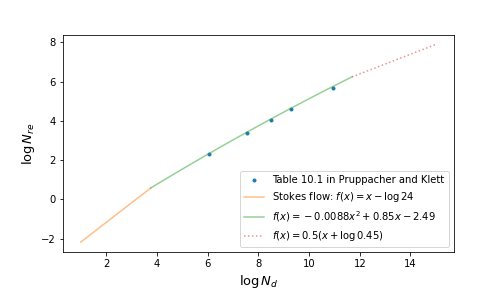
\includegraphics[width=\linewidth]{fig/clouds/davies_reynolds.png}
\caption{デービス数・レイノルズ数の関係.\label{fig:davies}}
\end{center}
\end{figure}

以上をまとめると
\begin{align}
\label{eq:vterm}
v_f =
\begin{cases}
&\displaystyle{\frac{2}{9 \eta} g r^2 (\delta_\cond - \rho) (1+1.26 N_{Kn}) } \nonumber \\
&\,\,\,\,\, \mbox{\, for $N_D < 42$ ($N_{re} < 2$)} \\
&\displaystyle{ \frac{\eta}{2 \rho r} \exp{(-0.0088 \log^2{N_D}+0.85 \log{N_D} -2.49)}} \nonumber \\
&\,\,\,\,\, \mbox{\, for $42 \le N_D < 10^5$ ($2 \le N_{re} < 500$)} \\
&\displaystyle{\frac{\eta}{2 \rho r} \sqrt{\frac{N_D}{C_d}}} \nonumber \\
&\,\,\,\,\, \mbox{\, for $10^5 \ge N_D$ ($500 \ge N_{re}$)} 
\end{cases}
\end{align}
となる。境界条件は接続するようにとっている。

\begin{figure}[htb]
\begin{center}
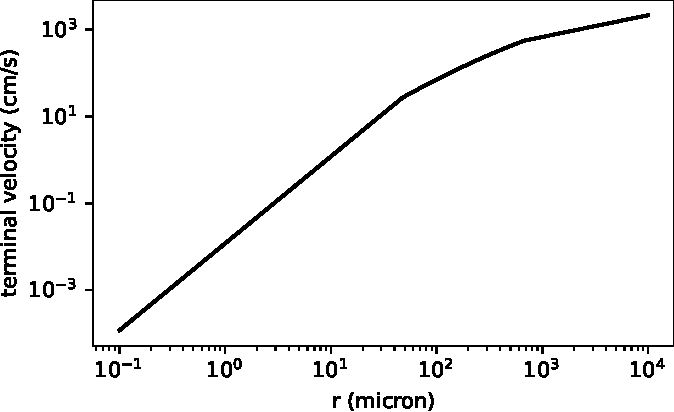
\includegraphics[width=\linewidth]{fig/clouds/vterm.pdf}
\caption{雲粒子半径と終端速度。地球大気・地球重力、$T=300$Kの場合。\label{fig:vterm}}
\end{center}
\end{figure}


\begin{itembox}{問題}
人間の会話や呼吸で排出される水について考えよう。WHOの定義では直径5\textmu m以上のの水滴をdroplet(飛沫)、直径5\textmu m以下の半径の水滴をaerosol(エアロゾル)あるいはdroplet nuclei(飛沫核)と定義している。地面から1.5mのところにある口から排出された直径5 \textmu mのエアロゾルは、何分くらい空気中に滞留するか?ここでは空気の流れはなく、水滴の蒸発もないとする。
\end{itembox}







\subsection*{蒸気圧曲線と雲底面}

単一成分の気体-固体、気体-液体の相変化による雲を考える。雲はある高度以上で気体が固体または液体に相変化することで発生する。雲の生成・消滅は複雑な物理によるが、ここでは蒸気圧曲線と分圧が一致した高さを雲底を簡単に定義する。すなわち気体成分の体積混合率を$\xi_v(P)$とすると
\begin{align}
P(T) = P_\mathrm{sat}(T)/\xi_v(P)
\end{align}
となる$(P,T)$が雲底であるとする(図\ref{fig:pbase})。また蒸気圧$P_\mathrm{sat}(T)$はClausius-Clapeyronの式から潜熱$l$を用いて
\begin{align}
P_\mathrm{sat}(T) = P_\mathrm{sat,0} e^{-l/RT}
\end{align}
の形で書ける(系外惑星探査6.2.3 p153)。


複数成分の気体からなる雲の場合、"気体成分"の体積混合比$\xi_v(P)$をどのように求めるかという問題もある。化学平衡計算をして求めるか、もしくは作れる最大の量を作るという考えかたもある。後者の場合、たとえばエンスタタイト($\mathrm{Mg Si O_3}$)であれば、それぞれの元素の体積混合比からの律速量を利用して
\begin{align}
\xi_v = \mathrm{min} [ \xi(\mathrm{Mg}),\xi(\mathrm{Si}),\xi(\mathrm{O})/3 ]
\end{align}
となる。

%Ackerman and Marley cloud model.ipynb (exojax)
\begin{figure}[htb]
\begin{center}
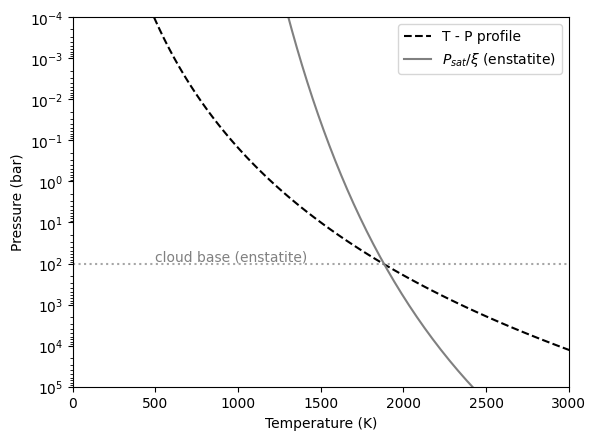
\includegraphics[width=\linewidth]{fig/clouds/pbase.png}
\caption{雲底の決め方。温度圧力プロファイルと蒸気圧曲線を体積混合率で割ったものとの交点が雲底となる。\label{fig:pbase}}
\end{center}
\end{figure}

\subsection*{Ackerman and Marleyの雲分布モデル}


系外惑星や褐色矮星の雲のモデルとしてよく用いられるAckerman \& Marley (2001)\cite{ackerman2001precipitating}(AM01)に基づき、いくつか修正して解説したい。
簡単のためある分子が凝縮して雲になることを考える。例えば水による雲は大気中では気体の状態($\vapor$)と雲の状態($\cond$)の二種類をとる。二つの状態の総和を$\total$で表す。混合比は混乱を避けるため体積混合比\footnote{体積混合比、すなわち数混合比では、一個をどう数えるか定義しなくてはならない。例えば、雲全体が含む分子の個数の場合もあれば、それぞれ大きさの違う(つまり含む分子の個数が異なる)雲粒子の個数の総和を想定する場合もありうる。}ではなく質量混合比で考える。
全質量混合比$X_\total (z) $は、雲の質量混合比$X_\cond$とガスの質量混合比$X_\vapor (z)$の和である。
\begin{align}
%\xi_m_\total (z) = \xi_m_\cond (z) + \xi_m_\vapor (z)
X_\total (z) = X_\cond (z) + X_\vapor (z)
\end{align}

このモデルではまず、代表サイズの雲粒子を考え、鉛直方向の輸送と降雨による凝縮体の沈降のバランス
\begin{align}
\label{eq:AM01}
%- \Kzz \frac{\partial}{\partial z} {\xi_m_\total (z)} - \overline{v}_f (z) \xi_m_\cond (z) = 0
- \Kzz \frac{\partial}{\partial z} {X_\total (z)} - \overline{v}_f (z) X_\cond (z) = 0
\end{align}
が基本的な式となる。ここに$\Kzz(z)$は鉛直方向の渦拡散係数(単位は$\mathrm{cm^2/s}$)、$\overline{v}_f(z)$は 雲粒子の典型的沈降速度である。


式(\ref{eq:AM01})を解くためには、$X$の三状態についてもう一つ拘束条件が必要である。ここでは
\begin{align}
%\xi_m_\cond (z)/\xi_m_\total (z) = \mathrm{const.} \equiv k_c
X_\cond (z)/X_\total (z) = \mathrm{const.} \equiv k_c
\end{align}
と仮定しよう。すると微分方程式(\ref{eq:AM01})は
\begin{align}
\label{eq:AM01c}
\frac{\partial}{\partial z} {X_\cond (z)} = - \frac{ k_c \overline{v}_f (z)}{\Kzz(z)} X_\cond (z) 
\end{align}
となる。

式(\ref{eq:AM01c})をみると$\overline{v}_f (z) \propto \Kzz(z)$と仮定できれば、この微分方程式は簡単に解けることがわかる。AM01ではそのような仮定を課しているようだ。つまり、沈降速度$\overline{v}_f(z)$が鉛直渦の速度スケール$v_\mathrm{eddy}(z) = \Kzz(z)/L$、ここに$L$は対流の典型的スケールに比例するとし、ここでは定数であるとする\footnote{AM01ではこれを定数としない定式化もなされている。定数としたものをHeuristicな場合として提示されている。}。$\fsed$を定数として
\begin{align}
\overline{v}_f(z) = \fsed v_\mathrm{eddy}(z) = \fsed \Kzz(z)/L \mbox{\,\,\,\,($\fsed$仮定)}
\end{align}
と書けるという仮定を置く。この場合、雲底より上の解は
\begin{align}
\label{eq:AM01cx}
X_\cond (z) = X_\cond(0) \exp{\left( - \frac{ k_c \fsed}{L} z \right) }
\end{align}
となる。

$L=H(z=0)=H_0$と仮定し、$z$と$P$の関係が$H_0$の静水圧で決まると仮定すると式(\ref{eq:AM01cx})は
\begin{align}
X_\cond(P) = 
\begin{cases}
X_\cond(0) \left( \frac{P}{P_0} \right)^{f_{sed}/k_c} & P \le P_0 \\
0 & P > P_0
\end{cases}
\end{align} 
と書ける。ここに$P=P_0$は雲底の圧力である。
雲の混合率分布は図\ref{fig:vmrcloud}のような分布となる。

%Ackerman and Marley cloud model.ipynb (exojax)
\begin{figure}[htb]
\begin{center}
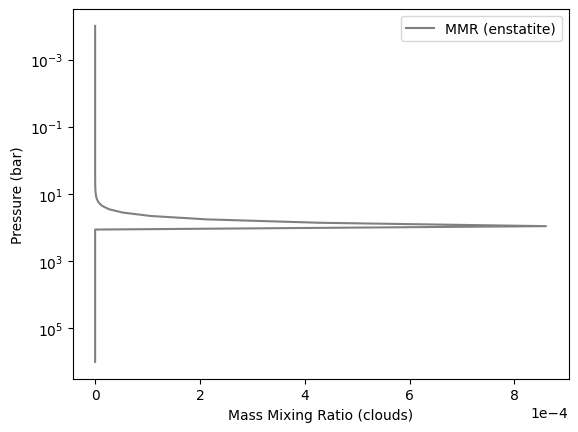
\includegraphics[width=\linewidth]{fig/clouds/mmrcloud.png}
\caption{雲の質量混合率の例。\label{fig:vmrcloud}}
\end{center}
\end{figure}

雲粒子のサイズ分布モデルを導入する。単位雲粒子半径あたりの雲の粒子数密度を
\begin{align}
    q(r) \equiv  \frac{d \mathcal{N}_\cond (r)}{d r} 
\end{align}
と定義する。ここに$\mathcal{N}_\cond(r)$は半径が$r$以下である粒子の数密度である。すなわち
\begin{align}
    \int_0^\infty q(r) dr = \int_0^\infty \frac{d \mathcal{N}_\cond (r)}{d r} dr = \mathcal{N}_\cond (\infty) \equiv N
\end{align}
が雲粒子の総数密度となる。ここでガスの数密度の表記である$n$と記号を変えている理由は、これは雲粒子の分子の数を数えているわけではないからであるという点に注意が必要である。雲粒子を構成する分子の数密度を$n_\cond$と表記すると、こちらは質量混合比と
\begin{align}
    X_\cond = \frac{\rho_\cond}{\rho} = \frac{\mu_\cond}{\mu} \frac{n_\cond}{n} 
\end{align}
の関係にある。${\mu_\cond}$は雲の構成分子の分子量である。ここに$\rho_\cond$は大気中で雲粒子全体が占める質量密度である($\mathrm{g/cm^3}$)。雲粒子自体の質量密度$\delta_\cond$と混同しないように注意が必要である(同じく単位は$\mathrm{g/cm^3}$)

また、$m_\cond$を雲粒子一つ一つの質量と定義すると、$dm_\cond/dr$が半径ごとの雲粒子の質量分布関数となる。雲粒子が球形であると仮定すると
\begin{align}
    \frac{dm_\cond}{dr} = \frac{4}{3} \pi r^3 \delta_\cond \frac{d \mathcal{N}_\cond (r)}{d r} = \frac{4}{3} \pi r^3 \delta_\cond q(r)
\end{align}
となる。

渦拡散係数と各粒子サイズ$r$における沈降速度$v_f(z; r)$が個別に与えられうるが、個別に与えた場合はこの「$\fsed$仮定」は一般にはなりたたない。

$\fsed$仮定を成り立たせるための一番強い仮定は各サイズに対して、
\begin{align}
v_f(z; r)= \fsed v_\mathrm{eddy}(z) = \fsed \Kzz(z)/L 
\end{align}
としてしまうことだが、これだと沈降速度のサイズ依存性を取り込めない。そもそも式(\ref{eq:AM01})は各粒子サイズに対して成り立つとしているわけではなく、なんらかの代表値でなりたつとしている。そこで$\fsed$仮定を代表操作に押し付けることになる。

いま沈降速度に対する代表操作を質量平均とする。すなわち
\begin{align} 
\label{eq:fsedw}
&\overline{v}_f(z) = \frac{\int v_f(m_\cond) dm_\cond}{M_c(z)} = \frac{\int_0^\infty v_f(z; r) (dm_\cond/dr) dr}{ \int_0^\infty (dm_\cond/dr) dr } \nonumber \\
&= \frac{\int_0^\infty dr \, v_f(z;r) r^3 q(r)}{ \int_0^\infty dr \, r^3 q(r)}
\end{align}
で対応付けられるとする。


高さ$z$の大気層において単位体積あたりの雲粒子の総質量は$M_c(z) = X_\cond(z) \rho $、ただし$\rho$は大気質量密度であることに注意。
%\begin{align} 
%M_c(z) 
%= \xi^c(z) m_c n_a = \xi^c(z) (\mu_\cond m_H) \frac{\rho}{\mu m_H}
%= \xi^c(z) (\mu_\cond/\mu) \rho = \epsilon \, \xi^c(z) \rho
%= X_\cond(z) \rho
%\end{align}
%$n_a$は大気全体の数密度、$m_c$は平均雲粒子質量、$m_H$は原子質量単位、$\mu_\cond$は雲粒子の平均分子量, $\mu$は大気全体の平均分子量、$\rho$は大気質量密度である。
%\begin{align} 
%\epsilon \equiv \mu_\cond/\mu
%\end{align}
%と定義した。
これが$\fsed$仮定を満たせばいいので
\begin{align} 
\label{eq:fsedw2}
\fsed \Kzz(z)/L = \frac{\int_0^\infty dr \, v_f(z;r) r^3 q(r)}{ \int_0^\infty dr \, r^3 q(r)}
\end{align}
となる必要がある。




AM01では$z$の層の雲粒子のサイズ分布として、対数正規分布
\begin{align} 
\label{eq:lognormal_am01}
%\left( q(r) \right) dr &= N(z) p_z(r) dr \mbox{\,\,\,(対数正規サイズ分布仮定)} \\
&q(r) dr = N(z) p_z(r) dr \mbox{\,\,\,(対数正規サイズ分布仮定)} \\
&p_z(r) = \nonumber \\
&\frac{1}{r \sqrt{2 \pi} \log{\sigma_g}} \exp{\left\{ - \frac{1}{2 (\log{\sigma_g})^2} \left[\log{\left(\frac{r}{r_g(z)}\right)}\right]^2 \right\}} 
\end{align}
を仮定する。ただし$\log{\sigma_g}>0$ ($\sigma_g>1$)である\footnote{通常、対数正規分布の記号は、ここでの$\log{\sigma_g}$を$\sigma$と置くが、ここではAM01に合わせている。少し混乱のもとであることは否めない。}。
$\sigma_g$が分布広がりを表現するが、ここでは各層で共通の値を採用していることに注意する。対数正規分布のモーメント公式
\begin{align} 
E_k \equiv \int_0^\infty dr r^k p_z(r) = r_g^k(z) e^{k^2 \log^2{\sigma_g}/2}
\end{align}
を用いると
\begin{align} 
&M_c(z) = X_\cond \rho  = \int dr \, \frac{4 \pi \delta_\cond r^3}{3} q(r) \nonumber \\
&= N(z) \frac{4 \pi \delta_\cond r_g^3(z)}{3} \exp{\left(\frac{9}{2} \log^2 \sigma_g\right)} 
\end{align} 
より、粒子の個数密度である$N(z)$が
\begin{align}
\label{eq:lognormal_am01N}
N(z) &= \frac{X_c \rho}{\tilde{m}} \\ 
\label{eq:lognormal_mean_mass}
\tilde{m} &\equiv \frac{4 \pi r_g^3}{3} \delta_c \exp{\left(\frac{9}{2} \log^2{\sigma_g} \right)}  
%\frac{3 X_\cond (z)}{4 \pi r_g^3(z)} \frac{\rho}{\delta_\cond } \exp{\left( - \frac{9}{2} \log^2{\sigma_g} \right)}  
\end{align}
と表されることが分かる。ここに$\tilde{m}$は、雲質量密度と雲粒子の個数密度をむすびつける粒子一個あたりの平均的な質量と解釈される。

さて$\fsed$仮定からくる要請(\ref{eq:fsedw2})から
\begin{align} 
\label{eq:xaxax}
 \int_0^\infty dr \, v_f(z;r) r^3 q(r) = \fsed \Kzz(z) E_3 /L 
\end{align} 
をみたす$v_f(r; z)$を仮定しないとならない。前節ではレイノルズ数によって傾きは若干変わるものの、終端速度はべき規則にほぼ従うことを見た。そこで、$v_f(r; z)$として、べき分布を仮定する
\begin{align} 
v_f(r,z) = A r^\alpha \mbox{\,\,\,(沈降速度べき仮定)}
\end{align} 

式(\ref{eq:xaxax})より、
\begin{align} 
\label{eq:xaxax2}
 A &= \frac{\Kzz(z)}{r_g^\alpha(z)} \frac{\fsed}{L} \frac{E_3}{E_{\alpha+3}} \nonumber \\
 &= \frac{\Kzz(z)}{r_g^\alpha(z)} \frac{\fsed}{L} e^{ -(\alpha^2 + 6 \alpha) \log^2{\sigma_g}/2 }
\end{align} 
となるので、
\begin{align} 
\label{eq:xaxax2x}
 v_f(r;z) &= \frac{\Kzz(z)}{r_g^\alpha(z)} \frac{\fsed}{L} e^{ -(\alpha^2 + 6 \alpha) \log^2{\sigma_g}/2 } r^\alpha \\
  &= \frac{\Kzz(z)}{L} \left( \frac{r}{r_w(z)} \right)^\alpha
\end{align} 
ここに
\begin{align} 
\label{eq:lognormal_am01rg}
r_w(z) = r_g(z) \fsed^{-1/\alpha} \exp{\left[ \left(\frac{\alpha+6}{2} \right) \log^2{\sigma_g}\right]}
\end{align}
となる。つまりこのような分布関数であれば$\fsed$仮定がなりたつ。そもそも式(\ref{eq:xaxax2x})は、べき則なので$r_w(z)$は典型的なスケールを与えるわけではなく、あくまで単にある$z$において沈降速度が鉛直輸送と釣り合っている粒子サイズを与えているに過ぎない。

さて式を閉じるためには$r_g(z)$と$\alpha$がわからないとならない。$r_g(z)$は、第\ref{ss:termv}章で用いたような物理的な終端速度モデルで$v_f(r)$が$\Kzz(z)/L 
$となる$r$を$r_w$として,式(\ref{eq:vterm})から$r_g$を算出すればよい。またAM01では、この付近の$r$の第\ref{ss:termv}章で用いたような物理的な終端速度モデルの$r$依存性をフィットして$\alpha$を決めることが推奨されている。

\begin{itembox}{AM01雲モデル($k_c$,$\fsed$一定)の特徴}
$\fsed$,$\Kzz(z)$,$\sigma_g$,$k_c$が与えられれば、各層での雲の混合比の鉛直分布(\ref{eq:AM01cx})と対数正規分布を仮定した各層の雲粒子分布(\ref{eq:lognormal_am01},\ref{eq:lognormal_am01N},\ref{eq:lognormal_am01rg})が与えられる。
\end{itembox}

以上から、各層で各粒子サイズの存在量がわかったので、これらの散乱断面積(レイリー散乱もしくはミー散乱)を足し合わせることで、雲の断面積が計算されることがわかる。


\subsection*{サイズ依存性が無視できる場合の断面積}

消散係数$Q_e(r)$が雲粒子のサイズ$r$によらずに一定である場合の消散断面積を計算してみよう。すなわち
\begin{equation}
    Q_e (r) = Q_e \mbox{\,\,\,\,\,\, (一定)}
\end{equation}
吸収断面積、散乱断面積の場合も吸収係数$Q_a$, 散乱係数$Q_s$で置き換えることで同様の議論ができる。

\begin{align}
\overline{\sigma}_\mathrm{ext}(z) &= \frac{\int_0^\infty dr \, Q_e \pi r^2 q(r)}{N} \\
&=  Q_e \pi r_g^2(z) e^{2\log^2{\sigma_g}} = Q_e \pi \overline{r}_\mathrm{geo}^2 
\end{align}
となる。ここに平均幾何半径
\begin{align}
\overline{r}_\mathrm{geo} \equiv e^{\log^2{\sigma_g}} r_g = r_w(z) \fsed^{1/\alpha} e^{-\frac{\alpha+4}{2} \log^2{\sigma_g}} 
\end{align}
を定義した。

さて大気各層のoptical depthは以下のように計算される。まず
\begin{align}
d \tau &= \int_0^\infty dr \, Q_e \pi r^2 q(r) d z = N \overline{\sigma}_\mathrm{ext}(z) dz \\
&= Q_e \pi \overline{r}_\mathrm{geo}^2 N dz  
\end{align}
となっていることを確認する。これは平均幾何半径と粒子数密度で表したoptical depthである。式(\ref{eq:lognormal_am01N},\ref{eq:lognormal_mean_mass})により、粒子数密度$N$から質量密度をもちいた表式に変換できる。すなわち
\begin{align}
\label{eq:dtaucloud0}
d \tau &= \frac{3  \rho Q_e }{4 \delta_\cond r_g(z)} \exp{\left[ - \frac{5}{2} \log^2{\sigma_g} \right]}  X_\cond (P) dz \\
&= X_\cond  (z) \frac{3 \rho Q_e }{4 \delta_\cond r_w(z) \fsed^{1/\alpha}}  \exp{\left[ \left( \frac{\alpha + 1}{2} \right) \log^2{\sigma_g} \right]} dz \\
\label{eq:dtaucloud1}
&= \frac{3 Q_e X_\cond  (z) \rho}{4 \delta_\cond r_\mathrm{eff}(z)} 
dz 
\end{align}

最後の式はAM01に従って実効半径を
\begin{align}
r_\mathrm{eff}(z) &\equiv r_w(z) \fsed^{1/\alpha} \exp{\left[ - \left( \frac{\alpha + 1}{2} \right) \log^2{\sigma_g} \right]} \\
&= r_g(z)  \exp{\left[ \frac{5}{2} \log^2{\sigma_g} \right]}
\end{align} 
と定義したものを使用したバージョンである。この定義は平均幾何断面積とは一致しないことに注意。



また、式(\ref{eq:dtaucloud0})を式(\ref{eq:pressureeq_})を用いて圧力座標に変換しておくと
\begin{align}
d \tau &=  \frac{3 Q_e X_\cond (z)}{4 r_g \delta_\cond g}  \exp{\left(- \frac{5}{2} \log^2{\sigma_g}\right)} dP
\end{align}
が得られる。最後の式は、インプットとして($r_g, \sigma_g)$を用いることに注意した定式である。

全体としては、
\begin{align}
\tau &= - \int_0^{P_0} X_\cond (P) \frac{3  Q_e \rho}{4 \delta_\cond r_\mathrm{eff}} \left( \frac{dz}{dP} \right) dP \\
&=  X_\cond (0) \int_0^{P_0}  dP \frac{3 Q_e \rho}{4 \delta_\cond r_\mathrm{eff}}  \frac{H}{P} \left( \frac{P(z)}{P_0} \right)^{f_{sed}/k_c}\\
&\approx   \frac{3}{4} \frac{ Q_e X_\cond(0) P_0}{ \delta_\cond g  r_\mathrm{eff} (1 + \fsed k_c) }
\end{align} 
となる\footnote{対応するAM01の(18)は$1/\delta_\cond$が抜けた誤植である。}。最後の式変形は$P_0/H = g \rho_0$と$\rho \approx \rho_0$を用いた (系外惑星探査 p137 6.5, 6.6.及び p139 6.28)。

一般には$Q_e$はサイズ依存性があるが、例えば、大きい粒径の極限では消散係数$Q_e \to 2$となるため、これを代入したものは幾何学的断面積となる。

\subsection*{Mie散乱の場合の断面積}

一般にはMie散乱から計算される粒子サイズに依存する$Q_e(r)$を用いて
\begin{align}
d \tau &= \int_0^\infty dr \, Q_e (r) \pi r^2 q(r) d z 
\end{align}
optical depthが計算される。Mie散乱の計算は大変であるが、幸い簡単に利用可能なソフトウェアが存在するので、それを利用するのもよいだろう。たとえば{\sf PyMieScatt}はPythonベースのMie散乱計算コードである。




\chapter{スペクトルからの大気推定}

スペクトルから惑星大気の諸量を推定する手順は大まかには以下のとおりである。
\begin{enumerate}
    \item 大気理論モデルの設定:パラメタを持つ大気モデルを作成し、モデルからスペクトルを生成できるコードを作成する
    \item 確率モデルの設定:スペクトルデータに付随する誤差モデルと大気モデルの事前分布を設定する 
    \item ベイズ推定の遂行:実スペクトルデータと生成したスペクトルから尤度を計算し、大気モデル中のパラメタの事後確率分布を求める
\end{enumerate}

大気理論モデルは、最も物理化学過程を含まないフリーリトリーバルでは、温度圧力分布自体を推定する。適当なパラメトライズモデルかガウス過程を用いたより自由なプロファイルを仮定することもできる。分子の存在量もパラメタとすることもできる。また高温系では熱化学平衡を仮定して、元素存在量を推定パラメタとすることも可能である。

大気理論モデルが設定されたら、次にスペクトルを生成する。以下ではこのスペクトル生成部分を詳述する。また、推定ではオパシティ計算が計算速度や精度を律速することが多い。そこでオパシティ計算の実際的手法も解説する。ベイズ推定の部分は第\ref{ch:infer}章と基本的には同様である。

\section{透過光スペクトルのモデリング}

\begin{figure*}[htb]
\begin{center}
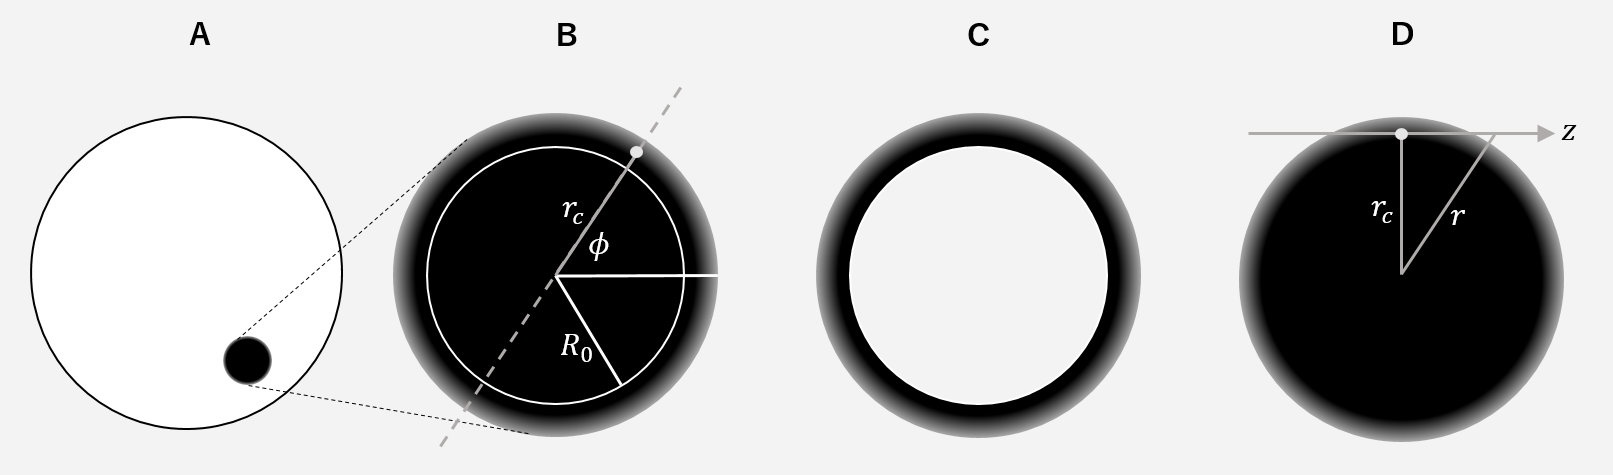
\includegraphics[width=0.85\linewidth]{fig/transmission_chord.PNG}
\caption{透過光分光を考えるための座標系。A:恒星の前面を通過する惑星。B:惑星部分の拡大図。C:円環影部分。D:中の破線方向に惑星を切断したときの図。恒星光の通過方向である$z$方向を弦方向と呼んでいる。右図は「系外惑星探査」図4.13に対応している。\label{fig:transmission_chord}}
\end{center}
\end{figure*}

図\ref{fig:transmission_chord}がトランジット時の概念図である。
透過光で問題になるのは惑星半径付近の薄い大気層での透過率の波長依存性である。そこで、十分透過率が低い位置の基準半径$R_0$を定めてそこから上層までの大気層の円環成分(図\ref{fig:transmission_chord}C)の実効的な影面積$A(\lambda)$(以降、円環影と呼ぶ)を考える。


例えばトランジット深さだけ考える場合、波長$\lambda$での惑星半径と恒星半径を$R_p(\lambda)$,$R_\star(\lambda)$であるとして
\begin{align}
\delta(\lambda) = \frac{R_p^2(\lambda)}{R_\star^2(\lambda)}  = \frac{\pi R_0^2 + A(\lambda) }{\pi R_\star^2(\lambda)}    
\end{align}
が観測量となり、円環影部分のみを考えればよい\footnote{Ingress/Egressを考える場合は円環影の一部分しか透過光に寄与しないためより複雑となるがここでは考えない。}。



さて一般に円環影部分(図\ref{fig:transmission_chord}C)の計算を考えよう。
座標系を図\ref{fig:transmission_chord} B/Dのように取る。
円環影部分は
\begin{align}
A &= \int_0^{2 \pi} \int_{R_0}^\infty [ 1 - \mathcal{T}_\lambda(r_c, \phi)] r_c d r_c d\phi \nonumber \\
&= \pi \left( 2 \int_{R_0}^\infty [ 1 - \mathcal{T}_\lambda(r_c, \phi)] r_c d r_c  \right)
\end{align}
また、
\begin{align}
    \label{eq:rp_trans}
    R_p(\lambda) = \sqrt{ R_0^2 + 2 \int_{R_0}^\infty [ 1 - \mathcal{T}_\lambda(r_c, \phi)] r_c d r_c }
\end{align}
とあらわされる。ここに$\mathcal{T}_\lambda(r_c, \phi)$は、ある波長$\lambda$における惑星ディスク半径$r_c$での弦方向の透過率である。$\mathcal{T}_\lambda(r)$は弦方向の光学的厚さ$t$と
\begin{align}
  \mathcal{T}_\lambda(r_c) = e^{-t}
\end{align}
の関係にある。以降、表記の簡略化のため$\lambda$の添え字を省略する。

$t$は弦方向の座標を$z$と取り、
\begin{align}
    t(r_c) = \int_{-\infty}^\infty \kappa(r) \rho(r) dz = 2 \int_{0}^\infty \kappa(r) \rho(r) dz
\end{align}
である。さてこの積分を大気レイヤーモデルで評価していこう。$t_n$を$n$番目のレイヤーの弦方向のオパシティとする。
図\ref{fig:transmission_coord}より
\begin{align}
    t_n &= 2 \sum_k \kappa_k \rho_k \Delta z^{(n)}_k 
\end{align}
この$\Delta t^{(n)}_k$は$n$番目のレイヤにむかってはられた弦方向の$k$ - $k-1$間レイヤーのオパシティである。これを鉛直一次元方向のオパシティ$\Delta \tau_k = \kappa_k \rho_k \Delta r_k$と関係づけると
\begin{align}
    t_n &= \sum_k  C_{nk} \Delta \tau_k \\
    \label{eq:chord_geo_matrix}
    C_{nk} &\equiv \frac{2 \Delta z^{(n)}_k}{\Delta r_k}
    = 2 \frac{\sqrt{r_{k-1}^2 - r_{n}^2} - \sqrt{r_{k}^2 - r_{n}^2}}{r_{k-1} - r_{k}}
\end{align}
となる。また$r_{N-1}=R_0$である。ここに下三角行列であるChord Geometric matrix $C = \{ C_{nk} \}$を要素ごとに定義した。

$N$は総レイヤー数($n=0,1,\cdots,N-1$)とする。
各レイヤー(下側境界までの)半径とレイヤーの高さには
\begin{align}
r_{n-1} = r_n + \Delta h_n
\end{align}
の関係がある。境界条件は、大気レイヤーの最下層を$n=N-1$とし、$R_0 = r_{N-1}$を惑星中心から最下層の下側境界までの基準半径とする。$r_{N-1}$より下は光が全く透過しないとする。すなわち
\begin{align}
    r_{n} =
\left\{
\begin{array}{ll}
\sum_{j=N-1}^{n+1} h_j + R_0 & \mbox{\, for $j<N-1$} \\
R_0 & \mbox{\, for $j=N-1$} 
\end{array}
\right.
\end{align}
となる。また$n=0$のレイヤーの上側境界(Top of Atmosphere; TOA)が必要である。これは別途$r_\mathrm{top}$と表記する。

大気レイヤーは$(T_n,P_n)$で表記されているため、長さスケールをスケールハイトを用いて変換しないとならない
\begin{align}
\Delta h_n &=  H_n \frac{\Delta P_n}{P_n} \\
\label{eq:H_each}
 H_n &= \frac{k_B T_n}{g_n \mu_n m_H} 
\end{align}
また重力定数は
\begin{align}
g_n = \frac{G (M_p + \Delta M_n)}{r_n^2}
\end{align}
と表される。$\Delta M_n = \sum_{j=N-1}^n \Delta m_j$であり$m_j$は$j$番目のレイヤの持つ質量である。$\Delta M_n$自体は通常は$M_p$に比べて無視できるので考えなくても良いかもしれない。

数値的には最下層から順番に$n=N-1, N-2, \cdots, 0$について$\Delta h_n, r_n$を解いていけばよい。境界条件は$r_N = R_0, g_N = G M_p/r_N^2$である。また$h_0 = 0$として最上層のオパシティは含めない。また同時に各層ごとに$C_{nk}$を$k=n$から$k=N-1$まで計算をしておけば、Chord Geometric Matrix が計算できる\footnote{もちろん$r_n$を計算した後に式(\ref{eq:chord_geo_matrix})で一括で計算してもよい。}。このように$C$は三角行列である。

\begin{figure*}[htb]
\begin{center}
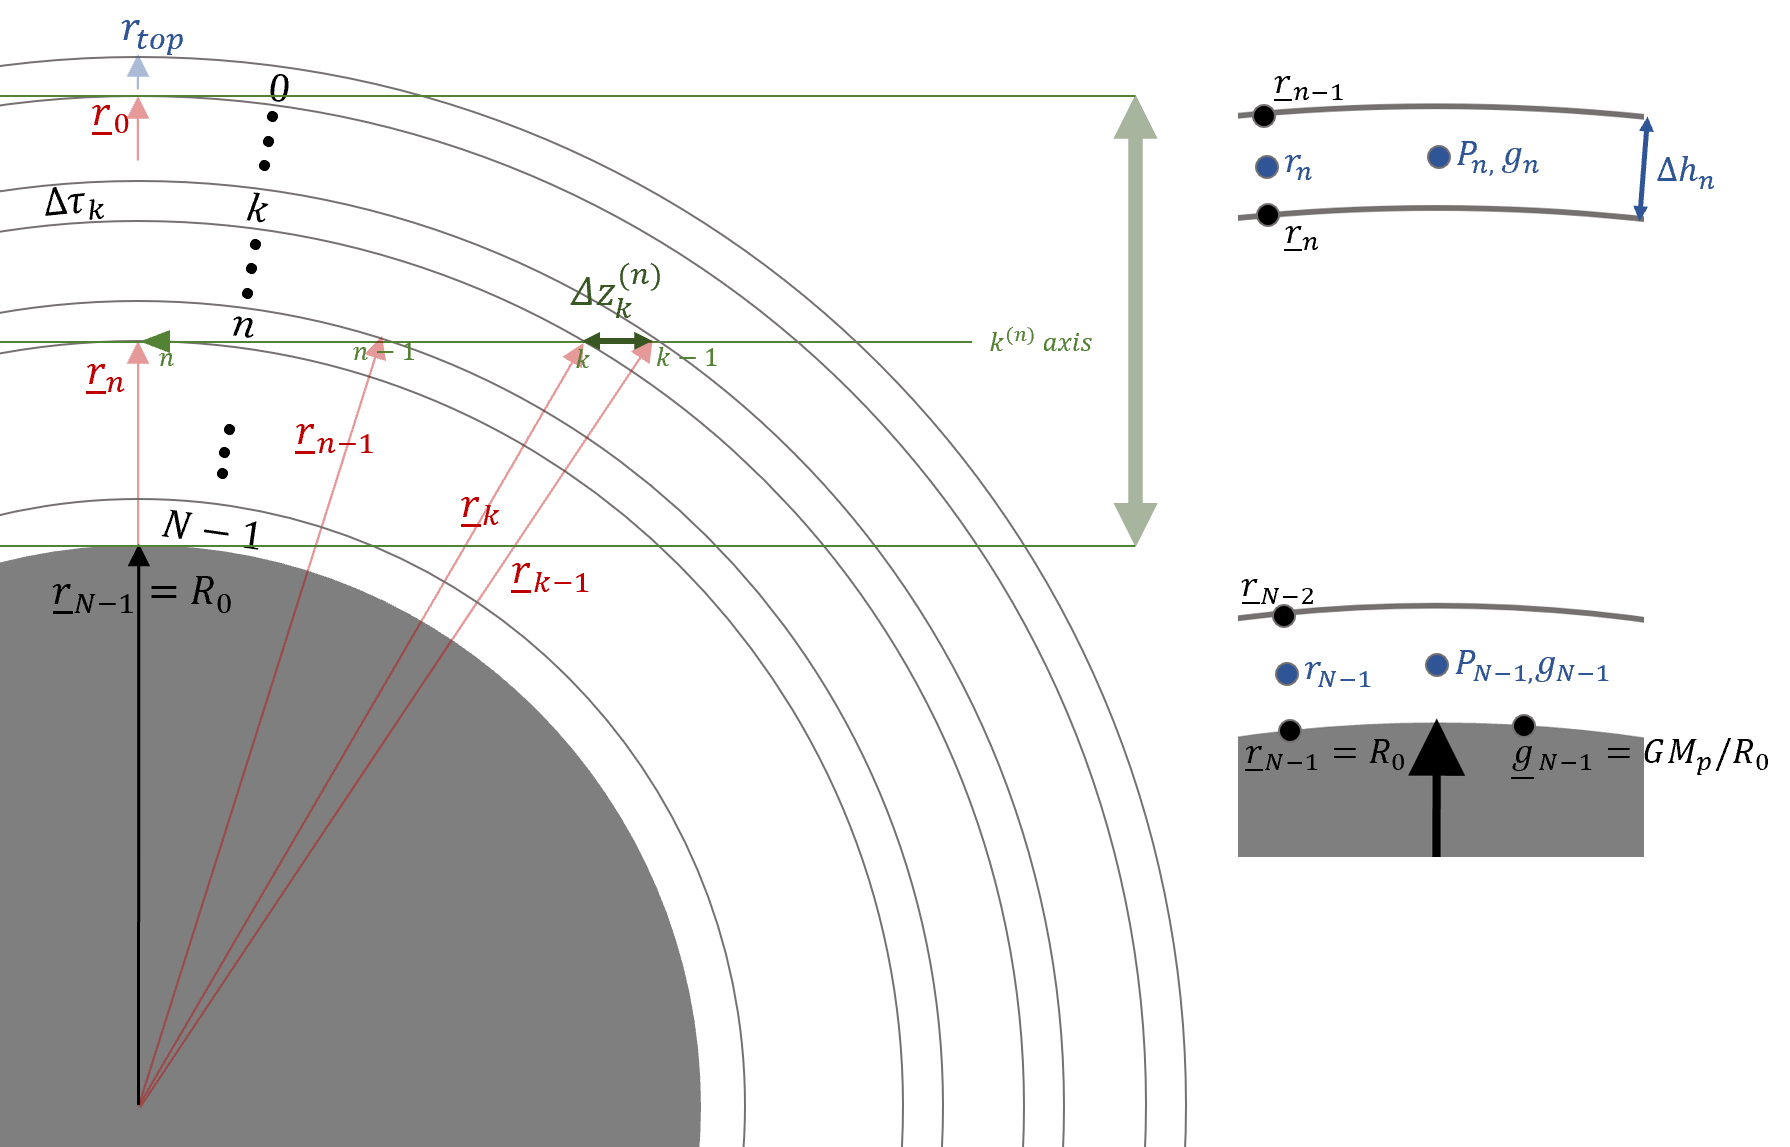
\includegraphics[width=1.0\linewidth]{fig/transmission_coord.PNG}
\caption{レイヤーモデルにおける光学的厚さの計算方向。\label{fig:transmission_coord}}
\end{center}
\end{figure*}

\section{Schwarzschild 方程式$^\ast$}
ある角度({\bf n})方向に、ある波数幅$d \nu$の間の光が微小面積($d S$、法線方向を${\bf k}$とする)・微小時間、微小立体角$d \Omega$内に伝達するエネルギーを$d {\mathcal{E}_\nu}$とすると、specific intensity $\Ilam$は以下のように表現される
\begin{align}
d {\mathcal{E}_\nu} = \Ilam ({\bf n} \cdot {\bf k})  d S d \Omega d \nu d t .
\end{align}

微小円柱に入射した光は$\Ilam$に比例して散乱・吸収する。比例定数をextinction coefficient (減光の係数という意味) \index{extinction coefficient@extinction coefficient} $\kappa_\nu$ という。ところで{\bf opacity}\index{opacity@opacity}という語は様々な定義で使われるが、この$[cm^2/g]$の次元を持つextinction coefficientをopacityと呼ぶことにする。また、今の意味ではopacityは単一周波数$\nu$に対して定義されているので厳密にはmonochromatic opacityである。何らかの周波数平均をした代表的なextinction coefficientもopacityと呼ぶ。このopacityを用いると、微小円柱内からの射出がない場合、単位時間内に吸収・散乱されるエネルギーは、微小距離$ds$、密度$\rho$を用いて、
\begin{align}
- \kappa_\nu \Ilam \rho d s d \Omega d \nu d t = d \Ilam d \Omega d \nu d t
\end{align}
となるので、
\begin{align}
d \Ilam = - \kappa_\nu \Ilam \rho d s
\end{align}
となる。微小円柱内からの射出放射輝度はemission coefficient \index{emission coefficient@emission coefficient} $\eta_\nu$を用いて
\begin{align}
d \Ilam =  \eta_\nu \rho d s
\end{align}
と定義するので、全体では
\begin{align}
d \Ilam = - \kappa_\nu \Ilam \rho d s + \eta_\nu \rho d s
\end{align}
となる。ここで放射源関数\index{ほうしゃげんかんすう@放射源関数}(source function) 
\begin{align}
\Jlam \equiv \frac{\eta_\nu}{\kappa_\nu}
\end{align}
を定義すると、放射伝達の式は
\begin{align}
\label{eq:radtran}
  \frac{d \Ilam}{\kappa_\nu \rho \, d s} = - \Ilam  + \Jlam
\end{align}
とかける。
さらに、光学的深さ
\begin{align}
d \tau = - \kappa_\nu \rho d z
\label{eq:opticalddef}
\end{align}
を定義することで、ある軸$z$をとって$ds = \mu dz$と$\mu=\cos{\theta}$を用いて
\begin{align}
\label{eq:radtrantau}
  \mu \frac{d \Ilam}{d \tau} = \Ilam  - \Jlam
\end{align}
となる。これをSchwarzschild equation\index{Schwarzschild equation@Schwarzschild equation}という。


電磁波の減光(extinction)には、光が吸収(absorption)され真に消失する効果と、異なる方向へと散乱(scattering)されて消失する効果の二種類の和
\begin{align}
\mathrm{extinction = absorption + scattering}
\label{eq:extsa}
\end{align}
となる。光子が原子・分子を電離し、原子の電離エネルギーと電離した電子の運動エネルギーとなる場合や、光子により原子・分子の電子が励起され、これが原子や分子同士の衝突により脱励起されることにより熱化する場合などは吸収に対応する。散乱は、光子が原子・分子の電子を励起した後、そのまま脱励起し同じ周波数の光子を出す場合や、電子、原子・分子による散乱などが含まれる。opacityの吸収、散乱による成分を、それぞれ、true absorption coefficient $\mu_a$ \index{true absorption coefficient@true absorption coefficient}とscattering coefficient $\mu_s$ \index{scattering coefficient@scattering coefficient}で表す。
\begin{align}
\kappa_\nu = \mu_a + \mu_s
\label{eq:extsaa}
\end{align}
となる。このとき、emission coefficientはmean intensity 
\begin{align}
{J_\nu} &\equiv  \langle \Ilam \rangle = \frac{1}{4 \pi} \int P(\Omega) d \Omega \Ilam
\end{align}
を用いて($P(\Omega)$は散乱の特性関数)
\begin{align}
\eta_\nu = \mu_a B_\nu + \mu_s {J_\nu}
\label{eq:emisaa}
\end{align}
と書ける。つまり放射源関数は
\begin{align}
\Jlam = \frac{\mu_a B_\nu + \mu_s {J_\nu}}{\mu_a + \mu_s} = (1 - \omega_0) B_\nu + \omega_0 {J_\nu}
\label{eq:sourcef}
\end{align}
と書ける。ここに
\begin{align}
\omega_0 \equiv \frac{\mu_s}{\mu_a  + \mu_s}
\label{eq:sia}
\end{align}
は単散乱アルベドと呼ばれる。つまり散乱のある場合の放射伝達式は、
\begin{align}
\label{eq:rtscat}
\Jlam = \omega_0 J_\nu + (1 - \omega_0 ) B_\nu
\end{align}
となる。

\section{輻射光スペクトルのモデリング}

輻射光スペクトルの生成は放射伝達を解く必要がある。しかし散乱を無視できる場合、比較的簡単な放射伝達計算となる。散乱無し(pure absorption)の場合、Schwarzschild方程式が形式的に積分可能となることからIntensityに関してレイヤー間を伝達させることができる。この場合、射出フラックスは、ToAでのIntensityを角度方向に積分することにより最後に計算する。

大気上端から取った鉛直方向のoptical depthを$\tau$とする。

Schwarzschild Equatuionは
\begin{align}
    \mu \frac{d I_\nu}{d \tau} = I_\nu - \mathcal{J}_\nu    
\end{align}
であるから、$\tau^\prime = \tau/\mu$と定義することで、$I_\nu$を$\mu$の関数として
\begin{align}
    \dot{I}_\nu(\mu) =  I_\nu (\mu) - \mathcal{J}_\nu (\mu)
\end{align}
とおける。両辺に$e^{-\tau^\prime}$をかけることで、$\tau^\prime = \tau_A^\prime $から$\tau^\prime = \tau_B^\prime$まで積分を実行することができ、形式解
\begin{align}
     I_\nu (\tau_B^\prime; \mu) e^{-\tau_B^\prime} = I_\nu (\tau_A^\prime, \mu) e^{-\tau_A^\prime} - \int_{\tau_A^\prime}^{\tau_B^\prime} \mathcal{J}_\nu (\mu)  e^{-\tau^\prime} d \tau^\prime
\end{align}
が得られる。これは積分系のSchwarzchild equationである。
%outgoing radiationを考えるので、$I_\nu(\tau;\mu)$の定義に符号反転したものを、$I^+(\tau;\mu)$とおく。
波数の添え字を省略する。また散乱無しの放射を考える($\omega_0=0$)ので、式(\ref{eq:rtscat})より、$\mathcal{J}_\nu (\mu)$は角度依存性のないプランク関数によって置き換えられる。


outgoingに寄与するintensityのみ、つまり$\mu \ge 0$のみを考えることにして$I(\tau, \mu)=I^+(\tau, \mu)$という表記を用いる\footnote{この意味では$\mu < 0$に対しては$I(\tau, \mu)=-I^-(\tau, \mu)$と定義される。}。ここである地点でoptical depthの基準をとり$\tau_B=0$として
\begin{align}
\label{eq:intensity_transfer}
         I^+ (0; \mu) = I^+ (\tau_A^\prime, \mu) e^{-\tau_A^\prime} +\int^{\tau_A^\prime}_{0} B_\nu (\tau) e^{-\tau^\prime} d \tau^\prime
\end{align}
が得られる。

式(\ref{eq:intensity_transfer})にて$\tau_A=\tau_s$ (下端)として、ある波数での放射伝達をTransmissionを$\mathsf{T}(z; \mu) \equiv e^{-\tau(z)/\mu}$として($z=0$が大気下端)、以下の量から計算することができる。
\begin{align}
    I^+(\mu) &= B_\nu(T_s) \mathsf{T} (z=0; \mu) + \int_0^\infty B_\nu(T) \frac{d \mathsf{T} (z)}{dz} dz 
%    &= B(T) e^{-\tau_s^\prime} + \int_0^\infty B(T) e^{-\tau^\prime} d \tau^\prime
\end{align}
$T_s$は大気下端温度, $\tau_s^\prime = \tau_s/\mu$と定義した。
上の式を$\mathsf{T}(z)$に関して離散化して
\begin{align}
    \label{eq:I_discrete_nemesis}
    I^+(\mu) &= B_\nu(T_s) \mathsf{T}_{N_\mathrm{layer}-1}(\mu) \nonumber \\
    &+ \sum_{j=0}^{N_\mathrm{layer}-1} B_\nu(T_j) (\mathsf{T}_{j-1}(\mu)- \mathsf{T}_j(\mu))
\end{align}
のように計算している\footnote{Irwin+では、大気下端から昇順にレイヤーインデックスを付与しているが、本文章では上端から昇順にインデックスを付与する。}。透過関数$\mathsf{T}_j = e^{\sum_{i=0}^j -\tau(z)/\mu}$であることからわかるように、式(\ref{eq:I_discrete_nemesis})の評価のために事前に透過関数を$0-j$まで計算しておく必要がある。

これを$\mu$について複数の求積点をもちいて計算する。
\begin{align}
    F^+(0) = 2 \pi \int_0^1 \mu I^+(\mu)  d \mu
\end{align}
これは$N$流の産卵なしのIntensityに戻づく輻射計算に対応し、散乱系への拡張はそのままでは困難である。


\section{散乱・反射スペクトルのモデリング (二流近似)$^\ddagger$}

さて散乱・反射がある場合、fluxに基づく二流近似がよく使われる。ここでは

平行平板の放射伝達の式は
\begin{align}
\mu \frac{d \Ilam}{d \tau} = \Ilam  - \Jlam
\label{eq:radtrantau_start}
\end{align}
であった。

まずextinctionとしては、吸収と散乱を両方考えることから
\begin{align}
\kappa_\nu = \mu_a + \mu_s
\label{eq:extsaa}
\end{align}
とおける。ここにtrue absorption coefficient $\mu_a$、(scattering coefficient $\mu_s$を用いている。

放射としては熱放射Cと下からの散乱Dを含めたものを考えよう。EからHまでは外からの光(外部光)を考えるケースであり、恒星の散乱光を考える場合に必要であるが今は考えない
この場合、emission coefficientは放射によるものと散乱によるものの和であるので
\begin{align}
\eta_\nu = \mu_a B_\nu + \mu_s \frac{1}{4 \pi} \int d \Omega \mathcal{P} (\Omega ) \Ilam
\label{eq:emisaa}
\end{align}
と書ける。右辺第一項では、第2項の散乱を無視した場合、吸収=放射(キルヒホッフの法則)となっている。すなわち局所熱力学平衡がなりたっているという仮定がおかれている\footnote{大気上層、例えば地球での中間圏あたりより上層ではこの仮定は成り立たない}。そのため、右辺第一項にプランク関数が現れている。局所熱力学平衡と詳細つり合いから導かれる強度分布がプランク分布だからである。
また、第2項は散乱を表す項であり、$\mathcal{P} (\Omega)  $は散乱の方向依存性をあらわす関数である。ここでは例えば薄い雲による散乱を想定しておこう。

放射源関数は
\begin{align}
\Jlam  = \frac{\eta_\nu}{\kappa_\nu} = (1 - \omega_0) B_\nu +   \frac{\omega_0}{4 \pi} \int d \Omega \mathcal{P} (\Omega ) \Ilam
\label{eq:sourcef}
\end{align}
ここに
\begin{align}
\omega_0 \equiv \frac{\mu_s}{\mu_a  + \mu_s}
\label{eq:sia}
\end{align}
は単散乱アルベドである。

モーメントを用いた記法、すなわち$\mu$の$n$乗をかけて立体角積分をした量(モーメント)を用いて、specific intensityの立体角方向の分布を表現する方法での記述が可能となる。全球面上での積分平均を定義しておこう:
\begin{align}
\label{eq:all_int}
  \langle\mathcal{F} \rangle&\equiv&  \frac{1}{4 \pi} \int d \Omega \mathcal{P} (\Omega ) \mathcal{F}  =  \frac{1}{4 \pi}  \int d \phi \int_{-1}^{1} d \mu \mathcal{P} (\Omega ) \mathcal{F} 
\end{align}
とする。0,1,2次のモーメントを次の記号で略記する。
\begin{align}
\Jl &\equiv \langle\Ilam \rangle\\
\Hl &\equiv \langle\mu \Ilam \rangle\\
\Kl &\equiv \langle\mu^2 \Ilam \rangle
\end{align}

0次のモーメントを用いて、放射源関数は
\begin{align}
\Jlam  = \frac{\eta_\nu}{\kappa_\nu} =  \omega_0 J_\nu + (1 - \omega_0) B_\nu 
\label{eq:sourcef}
\end{align}
と書ける。

放射伝達の式は
\begin{align}
\label{eq:rtbasic}
\mu \frac{d \Ilam (\Omega)}{d \tau} =  \Ilam (\Omega)  -   \omega_0 J_\nu - (1 - \omega_0) B_\nu 
\end{align}
となる。



二流近似では、これを上流側のフラックスと下流側に分けることを考える。
上半球(US)と下半球(LS)で積分する。今、モーメント方程式を意識して、任意の関数$\mathcal{F}$に対する積分平均演算子を
\begin{align}
\label{eq:us_int}
  \langle\mathcal{F} \rangle_\mathrm{US} &\equiv \frac{1}{4 \pi} \int_{\mathrm{US}} d \Omega \mathcal{P} (\Omega ) \mathcal{F}  \nonumber \\
  &=  \frac{1}{4 \pi}  \int d \phi \int_{0}^{1} d \mu \mathcal{P} (\Omega ) \mathcal{F} \\
\label{eq:ls_int}
  \langle\mathcal{F} \rangle_\mathrm{LS} &\equiv - \frac{1}{4 \pi}  \int_{\mathrm{LS}} d \Omega \mathcal{P} (\Omega ) \mathcal{F}  \nonumber \\
  &=  \frac{1}{4 \pi}  \int d \phi \int_{0}^{-1} d \mu \mathcal{P} (\Omega) \mathcal{F}   
\end{align}
と表記する。二流近似では下向きの量も正値になるように、後者には負号をつけて定義してあること、つまり
\begin{align}
\langle\mathcal{F} \rangle = \langle\mathcal{F} \rangle_\mathrm{US} - \langle\mathcal{F} \rangle_\mathrm{LS}
\end{align}
に注意する。さて大気にたいし上向きに射出するフラックスは、強度に対し上方向の角度依存性をかけ上半球について積分したものであるから、すなわち
\begin{align}
F^+ = \int_\mathrm{US} d \Omega \mu \, \mathcal{P} (\Omega ) \Ilam (\Omega) = 4 \pi   \langle \mu \Ilam (\Omega)  \rangle_\mathrm{US}
\end{align}
となる。$\Ilam (\Omega)=\Ilam (\mu)$と書ける。

いま等方散乱$\mathcal{P} (\Omega )=1$かつ強度のazimuth依存性が無視できるなら、
\begin{align}
F^+ = 2 \pi \int_0^1 d \mu \, \mu \,\Ilam (\mu)
\end{align}
となる。


\subsection*{散乱無しの直接解と透過関数}

式(\ref{eq:rtbasic})は散乱無し($\omega_0=0$)の場合、立体角のazimuth方向を無視し、$\mu$だけに依存するとする($\Ilam(\Omega) = \Ilam(\mu)$)と、両辺に$e^{-\tau/\mu}$を掛けて積分することにより$\Ilam(\mu)$について解析的に解ける。すなわち
\begin{align}
\label{eq:analypuabs}
\frac{d}{d \tau} \left( \Ilam(\tau,\mu) e^{-\tau/\mu} \right) = - \frac{B_\nu (T(\tau))}{\mu} e^{-\tau/\mu}
\end{align}
を$\tau$で積分すればよい。ここで図\ref{fig:layer1}のような、一層の大気層を考え、層の下部のintensityを$\Ilam(\tau_1,\mu) = \Ilams_1(\mu)$、上部を$\Ilam(\tau_2,\mu) = \Ilams_2(\mu)$とおく。式(\ref{eq:analypuabs})より
\begin{align}
\Ilams_1 (\mu) = \Ilams_2 (\mu) e^{-\Delta \tau/\mu} + \frac{1}{\mu} \int_{\tau_1}^{\tau_2} d \tau \Blam (T(\tau)) e^{- (\tau - \tau_1)/\mu}  
\end{align}
となる。ここに$\Delta \tau=\tau_2-\tau_1$である。層上部からの上向きフラックス$F_{+,1}$を、$2 \pi \mu$をかけて上半球で積分すると
\begin{align}
\label{eq:onelayer}
F_{+,1} &= 2 \pi \int_{0}^1 d\mu \mu \Ilams_1 (\mu) \\
&= 2 \pi \int_{0}^1 d\mu \, \Ilams_2 (\mu) \, \mu \, e^{-\Delta \tau/\mu} \nonumber \\
&+  \int_{\tau_1}^{\tau_2} d \tau \pi \Blam (T(\tau)) \mathcal{G} (\tau - \tau_1) \\
\mathcal{G} (\tau) &\equiv2 \int_{0}^1 d\mu \, e^{-\tau/\mu}
\end{align}
となる。この式は割と見通しが良い。すなわち上部から射出されるフラックスは、下部からの上向きの強度の伝達分($\Delta \tau/\mu$の減光を受けたものに対し$\mu$をかけ上半球積分したもの)と層内からの黒体輻射に対し順次、$\mathcal{G} (x)$(図\ref{fig:transrt}参照)の減光がかかって上部まで達したものの和となっている。特に大気上端を上部とし、すなわち$\tau_1=0$ととり, 下端からの放射を無視する、すなわち$\Ilam_2=0$ととった場合、式(\ref{eq:onelayer})は
\begin{align}
\label{eq:onelayer}
F_{+,1} = \int_{0}^{\infty} d \tau \pi \Blam (T(\tau)) \mathcal{G} (\tau) 
\end{align}
となる。

\begin{figure}[htb]
\begin{center}
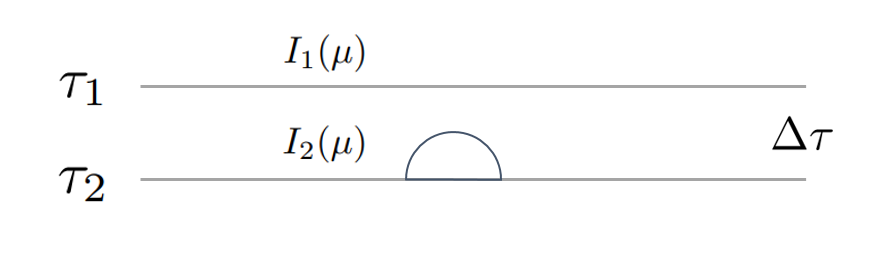
\includegraphics[width=\linewidth]{fig/layer1.PNG}
\caption{\label{fig:layer1}}
\end{center}
\end{figure}

\begin{figure}[htb]
\begin{center}
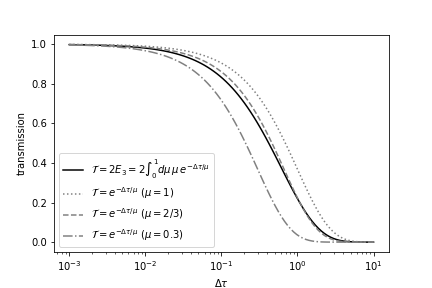
\includegraphics[width=\linewidth]{fig/transrt.PNG}
\caption{吸収のみの場合の透過関数。\label{fig:transrt}}
%exojax/examples/tutorial/pure\, absorption\, rt.ipynb
\end{center}
\end{figure}


散乱ありの場合との対応をとるために、式(\ref{eq:onelayer})を$F^+$の漸化式の形で書いてみよう。このために1-2間を大気中の薄い層とみなす。この層の中では温度一定とする。また下からの強度$\Ilams_2 (\mu)$の$\mu$依存性を無視すると
\begin{align}
\label{eq:onelayer}
F_{+,1} &= 2 \pi \Ilams_2  \int_{0}^1 d\mu \,  \, \mu \, e^{-\Delta \tau/\mu} + \pi \Blam (T) () \\
\end{align}


\subsection*{Moment Closureによる近似}

(e.g. Meadow \& Weaver 80 \cite{1980JAtS...37..630M}、Toon et al. 1989 \cite{1989JGR....9416287T}などを参照)。まず上半球(US)と下半球(LS)に対し、0次のモーメント(平均強度)
\begin{align}
\Jl_+ &\equiv \langle\Ilam \rangle_\mathrm{US} \\
\Jl_- &\equiv \langle\Ilam \rangle_\mathrm{LS} 
\end{align}
、一次のモーメント、
\begin{align}
\Hl_+ &\equiv \langle\mu \Ilam \rangle_\mathrm{US} \\
\Hl_- &\equiv \langle\mu \Ilam \rangle_\mathrm{LS} 
\end{align}
。また上向き下向きのフラックスは
\begin{align}
F^+ &= 4 \pi H_+ \\
F_- &= 4 \pi H_-
\end{align}
となる。

放射伝達の式は
\begin{align}
\label{eq:ratvvx}
 &\frac{d  }{d \tau} \langle\mu  \Ilam (\Omega) \rangle_\mathrm{US} \nonumber \\
 &=  \langle \Ilam(\Omega) \rangle_\mathrm{US}  - \omega_0 \langle \mu  \rangle_\mathrm{US} J_\nu - (1-\omega_0) \langle\mu \rangle_\mathrm{US} \Blam \\
 \label{eq:ratvv2x}
 &\frac{d  }{d \tau} \langle\mu^2  \Ilam (\Omega) \rangle_\mathrm{LS} \nonumber \\
 &=  \langle\mu \Ilam(\Omega) \rangle_\mathrm{LS} - \omega_0 \langle \mu \rangle_\mathrm{LS} J_\nu  - (1-\omega_0)\langle\mu \rangle_\mathrm{LS} \Blam  
 \end{align}
となる。ここで$\langle \mu \rangle_\mathrm{US}=-\langle \mu \rangle_\mathrm{LS}=1/2$であるから、
\begin{align}
\label{eq:ratvv}
 \frac{d  }{d \tau} \langle\mu  \Ilam (\Omega) \rangle_\mathrm{US}  &=  \langle\Ilam(\Omega) \rangle_\mathrm{US} - \frac{\omega_0}{2} J_\nu  - \frac{(1-\omega_0)}{2} \Blam  \\
 \label{eq:ratvv2}
 \frac{d  }{d \tau} \langle\mu  \Ilam (\Omega) \rangle_\mathrm{LS}  &=  \langle \Ilam(\Omega) \rangle_\mathrm{LS}  + \frac{\omega_0}{2} J_\nu - \frac{(1-\omega_0)}{2} \Blam  
 \end{align}

ここで$\Jl = \Jl_+ - \Jl_-$を用い、またclosure relationを
\begin{align}
\eta_+ &= \Jl_+/\Hl_+ \\
\eta_- &= - \Jl_-/\Hl_- 
\end{align}
と置くことで、

\begin{align}
\label{eq:ratvvA}
\dot{\Hl}_+ &= \eta_+ \left( 1 - \frac{\omega_0}{2}\right) \Hl_+ - \frac{ \omega_0}{2}  \Hl_- - \frac{(1-\omega_0)}{2} \Blam  \\
 \label{eq:ratvv2A}
 \dot{\Hl}_- &= \frac{\eta_+ \omega_0}{2} \Hl_+ -  \eta_- \left( 1 - \frac{ \omega_0}{2}\right) \Hl_- + \frac{(1-\omega_0)}{2} \Blam
 \end{align}
または
\begin{align}
\label{eq:ratvvA}
\dot{F}_+ &= \eta_+ \left( 1 - \frac{\omega_0}{2}\right) F^+ -  \frac{\eta_- \omega_0}{2}  F_- - 2 \pi (1-\omega_0) \Blam  \\
 \label{eq:ratvv2A}
 \dot{F}_- &= \frac{\eta_+ \omega_0}{2} F^+ -  \eta_- \left( 1 - \frac{ \omega_0}{2}\right) F_- + 2 \pi (1-\omega_0) \Blam
 \end{align}
となる。

ここで上半球と下半球のclosure relationが同じ形とおもうと$\eta_+ = \eta_- \equiv \eta$となり
\begin{align}
\label{eq:ratvvAaVV}
\dot{F}_+ (\tau) &= \gamma_1 F^+ (\tau) - \gamma_2  F_- (\tau) - 2 \pi (1-\omega_0) \Blam  (\tau) \\
 \label{eq:ratvv2A}
 \dot{F}_- (\tau) &=  \gamma_2 F^+ (\tau) - \gamma_1 F_- (\tau) + 2 \pi (1-\omega_0) \Blam (\tau)
 \end{align}
の形となる。ただし
\begin{align}
\gamma_1 &\equiv\eta \left( 1 - \frac{\omega_0}{2}\right) \\
\gamma_2 &\equiv\frac{\eta \, \omega_0}{2}
\end{align}
とおいた。$\gamma_1+\gamma_2=\eta$、$\gamma_1-\gamma_2=\eta (1-\omega_0)$である。

式(\ref{eq:ratvvAaVV},\ref{eq:ratvv2A})は一階の連立微分方程式であり、斉次系に$\Blam(\tau)$由来の$\tau$依存性のある項が付加されたものである。よって$\Blam(\tau)$をテイラー展開して打ち切り有限項の多項式に近似すれば解くことができる。


$\gamma_1 = 2 - \omega_0$、$\gamma_2 = \omega_0$ ととれば、半球平均近似(Hemispheric mean)かつ非対称パラメタ$g=0$の時と一致する \cite{1989JGR....9416287T}. 式 (\ref{eq:ratvvAaVV})、  (\ref{eq:ratvv2A})を解くために、 新たなパラメタ$\Fsum \equiv F^+ + F_-, \Fnet \equiv F^+ - F_-$ と定義し書き換えると以下を得る:
\begin{align}
%\dFnet &= \eta (1 - \omega_0) \Fsum - 4 \pi (1- \omega_0) \Bl\\
%\dFsum &= \eta \Fnet
\dFnet &= (\gamma_1 - \gamma_2) \Fsum - 4 \pi (1- \omega_0) \Bl\\
\dFsum &=  (\gamma_1 + \gamma_2)  \Fnet,
\end{align}
これより二階微分方程式
\begin{align}
%\ddFsum - \eta^2 (1 - \omega_0) \Fsum + 4 \pi (1-\omega_0) \Bl = 0.
\ddFsum - (\gamma_1^2 - \gamma_2^2)  \Fsum + 4 \pi (1-\omega_0) (\gamma_1 + \gamma_2) \Bl = 0.
\end{align}
が得られる。

ここで$\Bl$の変数$\tau$に対するテイラー展開の一次まで残すことを考えよう\cite{1989JGR....9416287T} \cite{heng2017exoplanetary}。
\begin{align}
\Bl \approx B_0 + \dot{B} (\tau - \tau_0).
\end{align}
この時、解は以下のように求まる。
\begin{align}
\Fsum &= c_1 e^{\lambda \tau} + c_2 e^{-\lambda \tau} +\frac{ 4 \pi (1-\omega_0)}{\gamma_1 - \gamma_2} \Bl \\
\Fnet &= c_1 \delta e^{\lambda \tau} - c_2 \delta e^{-\lambda \tau} +\frac{ 4 \pi (1-\omega_0)}{\gamma_1^2 - \gamma_2^2} \dBl,
\end{align}
%where $\lambda \equiv \eta (1-\omega_0)^{1/2}$. 
ここに
\begin{align}
\lambda &\equiv\sqrt{\gamma_1^2-\gamma_2^2} \\
\delta &\equiv\sqrt{\frac{\gamma_1 - \gamma_2}{\gamma_1 + \gamma_2}}.
\end{align}

上の解を$F^+$、$F_-$に戻すことで以下が求まる。
\begin{align}
F^+ (\tau) &= c_1 \zeta_+ e^{\lambda \tau} + c_2 \zeta_- e^{-\lambda \tau} + \pi \mathcal{B}_+ (\tau)  \\
F^- (\tau) &= c_1 \zeta_- e^{\lambda \tau} + c_2 \zeta_+ e^{-\lambda \tau} + \pi \mathcal{B}_- (\tau)
\end{align}
ここに
\begin{align}
 \mathcal{B}_\pm(\tau) &\equiv\frac{ 2 (1-\omega_0)}{\gamma_1 - \gamma_2} \left( \Bl(\tau) \pm \frac{1}{\gamma_1 + \gamma_2} \dBl (\tau) \right) \\
 \zeta_\pm &\equiv\frac{1}{2} (1 \pm \delta).
\end{align}
である。$\zeta_\pm$は結合定数と呼ばれる
 \cite{heng2017exoplanetary}.

\subsection*{大気レイヤーモデルの放射伝達の解法}

ここまではHemispheric meanの二流近似を導出してきたが、Toon89型の二流近似における上向きおよび下向きストリームの解は以下のように同様に表現できる。
\begin{align}
\label{eq:2stream_1}
F^+ (\tau) &= c_1 \zeta^+ e^{\lambda \tau} + c_2 \zeta^- e^{-\lambda \tau} + \pi \mathcal{B}^+ (\tau)  \\
\label{eq:2stream_2}
F^- (\tau) &= c_1 \zeta^- e^{\lambda \tau} + c_2 \zeta^+ e^{-\lambda \tau} + \pi \mathcal{B}^- (\tau)
\end{align}
ここで、$\zeta^\pm$は結合係数と呼ばれる。注目すべきことに、球面調和関数(SH)法の二流近似も同じ形をとる。そこでこの形の方程式から大気レイヤーモデルの放射伝達の解法を考えよう。

%omegaとgがgamma_1、gamma_2、zetaとどのように関連するか
上記の方程式において、$\zeta^{\pm}$と$\lambda$は、$F^{\pm}$の微分方程式の係数である$\gamma_1$と$\gamma_2$に以下のように関連している。
\begin{align}
    \zeta^\pm &= \frac{1}{2} \left( 1 \pm \sqrt{\frac{\gamma_1 - \gamma_2}{\gamma_1 + \gamma_2}} \right)\\
    \lambda &= \sqrt{\gamma_1^2 - \gamma_2^2},
\end{align}
係数$\gamma_1$と$\gamma_2$は、単一散乱アルベド$\omega$と非対称パラメータ$g$によって決定される。この関係はモーメント閉包の方法に依存する \cite{1989JGR....9416287T}。半球平均を使用する場合、
$\gamma_1 = 2 - \omega (1 + g)$および$\gamma_2 = \omega (1 - g) $
の関係が成り立つ。また、簡約化された源関数は以下のように表される
\begin{align}
\mathcal{B}^\pm (\tau) = 
    \frac{ 2 (1-\omega)}{\gamma_1 - \gamma_2} \left( \Bl(\tau) \pm \frac{1}{\gamma_1 + \gamma_2} \dBl (\tau) \right).
\end{align}
上記の方程式において、第二項は等温層の場合には無視される。

式 (\ref{eq:2stream_1}, \ref{eq:2stream_2}) は以下のように表現できる
\begin{align}
    \Fv(\tau) = Q(\tau) \xv + \pi \Bv (\tau)
\end{align}
ここで $\Fv (\tau) = (F^+ (\tau), F^-(\tau))^\top $、$\Bv (\tau) = (\mathcal{B}^+ (\tau), \mathcal{B}^- (\tau))^\top$、$\xv \equiv (c_1, c_2)^\top$、そして
\begin{align}
    Q(\tau) = \left(
\begin{array}{cc}
\zeta^+ e^{\lambda \tau} & \zeta^- e^{-\lambda \tau}  \\
\zeta^- e^{\lambda \tau} & \zeta^+ e^{-\lambda \tau}  \\
\end{array}
\right)
\end{align}

%\subsubsection*{均一層モデルの標準線形形式}
次に、光学的厚さの差$\Delta \tau_n$を持つ$N$層モデルを考え、第$n$層の上端における光学的深度を$\tau = \tau_n = \sum_{i=0}^{n-1} \Delta \tau_i$($n \ge 1$)および$\tau_0 = 0$として定義する。

第$n$層について考えよう。
\begin{align}
\label{eq:Fv1}
    \Fv (\tau_n) &= Q_n(\tau_n) \xv_n + \pi \Bv_n (\tau_n) = \Fv_n\\
\label{eq:Fv2}
    \Fv (\tau_n+\Delta \tau_n) &= Q_n(\tau_n + \Delta \tau_n) \xv_n + \pi \Bv_n (\tau_n + \Delta \tau_n) \nonumber \\
    &= \Fv_{n+1}
\end{align}
ここで$Q_n$は第$n$層の$Q(\tau)$として定義される。したがって、第$n$層の内部パラメータ$\zeta^\pm_n$と$\lambda_n$を設定すると、
\begin{align}
    Q_n(\tau) = \left(
\begin{array}{cc}
\zeta^+_n e^{\lambda_n \tau} & \zeta^-_n e^{-\lambda_n \tau}  \\
\zeta^-_n e^{\lambda_n \tau} & \zeta^+_n e^{-\lambda_n \tau}  \\
\end{array}
\right).
\end{align}

式 (\ref{eq:Fv1}) と (\ref{eq:Fv2}) から、漸化関係の線形形式を得る:
\begin{align}
    \label{eq:rtstandard}
    \Fv_{n+1} &= \mathcal{G} (\Delta \tau_n) \Fv_n + \pi \Gv_n,
\end{align}
ここで
\begin{align}
   \Gv_n \equiv \Bv_n (\tau_n + \Delta \tau_n) - \mathcal{G} (\Delta \tau_n) \Bv_n (\tau_n)  
\end{align}
かつ$\Gv_n = (G_n^+, G_n^-)^\top$である。
また、伝達関数を以下のように定義した
\begin{align}
\label{eq:transfer_matrix}
\mathcal{G} (\Delta \tau_n) &\equiv Q(\tau_n + \Delta \tau_n) Q^{-1}(\tau_n) \\
&=  Q_n(\tau_n)
 \left(
\begin{array}{cc}
e^{\lambda_n \Delta \tau_n}  & 0  \\
0 & e^{-\lambda_n \Delta \tau_n}  \\
\end{array}
\right) Q_n^{-1}(\tau_n) \nonumber \\
\end{align}
これは$ \mathcal{G} (\Delta \tau_n) \qv_i = \lambda^\prime_i \qv_i$の固有値分解であり、ここで$\qv_i$は$Q_n(\tau_n)$の第$i$列ベクトルである。したがって$\qv_i$を正規化でき、特に$\qv_1$を$e^{\lambda_n \tau_n}$で、$\qv_2$を$e^{-\lambda_n \tau_n}$で正規化できる。以下のように定義することで
\begin{align}
    Z_n \equiv Q_n(0) = \left(
\begin{array}{cc}
\zeta^+_n  & \zeta^-_n  \\
\zeta^-_n & \zeta^+_n  \\
\end{array}
\right),
\end{align}
上記の方程式を以下のように書き直せる
\begin{align}
\label{eq:transfer_matrix2}
&\,\mathcal{G} (\Delta \tau_n) = 
 Z_n
 \left(
\begin{array}{cc}
e^{\lambda_n \Delta \tau_n}  & 0  \\
0 & e^{-\lambda_n \Delta \tau_n}  \\
\end{array}
\right) Z_n^{-1} \\
\label{eq:gzero}
&= \frac{1}{{\zeta^+_n}^2 - {\zeta^-_n}^2} \nonumber \\
&\times \left(
\begin{array}{cc}
  {\zeta^+_n}^2 e^{t_n} - {\zeta^-_n}^2 e^{-t_n} & \,  - \zeta^+_n \zeta^-_n (e^{t_n} - e^{-t_n}) \\
\zeta^+_n \zeta^-_n (e^{t_n} - e^{-t_n})& \, {\zeta^+_n}^2 e^{-t_n} - {\zeta^-_n}^2 e^{t_n} \\
\end{array}
\right), \nonumber \\
\end{align}
ここで
\begin{align}
t_n \equiv \lambda_n \Delta \tau_n
\end{align}
は$\Delta \tau_n$の関数であるが、$\tau_n$の関数ではない。

等温層の場合、$\Bv_n (\tau_n) = \Bv_n (\tau_n + \Delta \tau) \equiv \mathcal{B}_n \uv$、$\mathcal{B}_n = \mathcal{B}^+ (\tau_n) = \mathcal{B}^- (\tau_n)$であり、ここで$\uv$は単位ベクトル$\uv \equiv (1,1)^\top$である。源行列$\Gv_n$は以下のように簡約化できる
\begin{align}
\Gv_n &= \mathcal{B}_n (I - \mathcal{G} (\Delta \tau_n) ) \uv \\
&= \frac{\mathcal{B}_n}{\zeta_n^+ + \zeta_n^-} \left(
\begin{array}{c}
     \zeta_n^+ (1 - e^{t_n}) + \zeta_n^- (1 - e^{-t_n}) \\
    \zeta_n^+ (1 - e^{-t_n}) + \zeta_n^- (1 - e^{t_n})
\end{array}
\right)
\end{align}
ここで$I$は単位行列である。

\subsubsection*{単一層内での伝達}

線形形式 (\ref{eq:rtstandard}) は数学的に簡潔であるが、その物理的意味は明確ではない。そこで、単一層内での光の伝達を表す形式に変換する。

式 (\ref{eq:rtstandard}) から以下が得られる
\begin{align}
    F^+_n = \Gaa^{-1} F^+_{n+1} - \Gaa^{-1} \Gab F^-_n -\Gaa^{-1} \pi G_n^+,
\end{align}
ここで$\mathcal{G}_{ij}$は記号から$n$を省略した$\mathcal{G}(\Delta \tau_n)$の$(i-j)$成分である。この方程式を
$F^-_{n+1} = \Gba F^+_{n} + \Gbb F^-_n + \pi G_n^-$に代入すると、以下を得る
\begin{align}
F^-_{n+1} &= \Gba \Gaa^{-1} F^+_{n+1} + (\Gbb - \Gba \Gaa^{-1} \Gab) F^-_n \nonumber \\
&+ \pi G_n^- - \Gba \Gaa^{-1} \pi G_n^+ .
\end{align}


二流の場合、式 (\ref{eq:gzero}) から$\Gba = -\Gab$かつ$\Gaa^{-1} = \Gbb - \Gba \Gaa^{-1} \Gab \equiv \mathcal{T}_n $および$\Gba \Gaa^{-1} = - \Gaa^{-1} \Gab \equiv \mathcal{S}_n $が導かれる。そこで、第$n$層内での放射伝達を以下のように表現できる
\begin{align}
\label{eq:twosq1}
 F^+_n &= \mathcal{T}_n F^+_{n+1} + \mathcal{S}_n F^-_n - \mathcal{T}_n \pi G_n^+ \\
 \label{eq:twosq2}
 F^-_{n+1} &= \mathcal{T}_n F^-_{n} + \mathcal{S}_n F^+_{n+1} + \pi G_n^- - \mathcal{S}_n \pi G_n^+,
\end{align}
ここで
\begin{align}
\label{eq:transmission_onelayer}
 &\mathcal{T}_n \equiv 
 \frac{{{\zeta^+_n}}^2 -{{\zeta^-_n}}^2 }{{\zeta^+_n}^2  - (\zeta^-_n\mathsf{T}_n)^2 } \mathsf{T}_n \\
 \label{eq:scattering_onelayer}
&\mathcal{S}_n  \equiv 
\frac{\zeta^+_n \zeta^-_n }{{\zeta^+_n}^2  - (\zeta^-_n\mathsf{T}_n)^2 } (1-\mathsf{T}_n^2)
 \end{align}
は層の底部と頂部間の透過率およびフラックスの反対方向からの散乱とみなすことができる\footnote{式 (\ref{eq:scattering_onelayer}) での散乱の不透明極限 ($\mathsf{T}_n =0$) を$S_\infty \equiv \zeta_-/\zeta_+$として定義すると、式 (\ref{eq:scattering_onelayer_}) を \cite{2023PSJ.....4...10R} でのflux-adding treatmentで使用されるものと同様の形に書き直すことができる:
\begin{align}
\label{eq:scattering_onelayer_}
 &\mathcal{T}_n = \frac{S_\infty ( 1 - e^{-2 \lambda_n \Delta \tau_n})}{1 - S_\infty^2  e^{-2 \lambda_n \Delta \tau_n} }. 
 \end{align}
 半球平均の場合、以下を得る
 \begin{align}
     S_\infty &= \frac{\sqrt{1-\omega g}-\sqrt{1-\omega}}{\sqrt{1-\omega g}+\sqrt{1-\omega}} \\
     \lambda_n &= 2 \sqrt{(1-\omega g)(1-\omega)}.
 \end{align}
 } 。上記の式において、透過関数を定義した \cite{heng2017exoplanetary}:
 \begin{align}
 \label{eq:opacity_transfer}
 \mathsf{T}_n &\equiv e^{-\lambda_n \Delta \tau_n} 
% \delta_n &\equiv{{\zeta^+_n}}^2 -{{\zeta^-_n}}^2  \\
% \theta_n &\equiv\zeta^+_n \zeta^-_n.
\end{align} 
式 (\ref{eq:twosq1}, \ref{eq:twosq2}) は本質的に \cite{heng2017exoplanetary} によって導出された二流近似の解析的表現と同じであることに注意されたい\footnote{\cite{heng2017exoplanetary} の式 (3.58)。我々の形式での$\lambda_n$は \cite{heng2017exoplanetary} での$\mathcal{D}$に対応する。}。

等温層の場合、式 (\ref{eq:twosq1}) と (\ref{eq:twosq2}) を以下のように簡約化できる
\begin{align}
\label{eq:twosq1iso}
 F^+_n &= \mathcal{T}_n F^+_{n+1} + \mathcal{S}_n F^-_n + \pi \hat{\mathcal{B}}_n\\
 \label{eq:twosq2iso}
 F^-_{n+1} &= \mathcal{T}_n F^-_{n} + \mathcal{S}_n F^+_{n+1} + \pi \hat{\mathcal{B}}_n
\end{align}
ここで
\begin{align}
    \hat{\mathcal{B}}_n \equiv (1 - \mathcal{T}_n - \mathcal{S}_n) \mathcal{B}_n.
\end{align}


\subsection*{flux-adding treatment}\label{ss:flux-adding}

散乱を含む二流近似の解法として、反射の形式を利用するflux-adding treatment \cite{2018JQSRT.211...78R,2023PSJ.....4...10R} が提案されている。これは古典的な加算技法から類推的に導出される。flux-adding treatmentは、与えられた層における上向きフラックスが、下向きフラックスの反射と層からの源項の和として表現できると仮定する。
\begin{align}
    \label{eq:fa1}
    F_n^+ &= \hat{R}_n^+ F_n^- + \hat{S}_n^+ \\
    \label{eq:fa2}
    F_n^- &= \hat{R}_n^- F_n^+ + \hat{S}_n^-.
\end{align}

式 (\ref{eq:twosq1iso}) 中の$F_n^+$を式 (\ref{eq:fa1}) で置き換え、$\mathcal{T}_n$を乗じると、以下の式が導かれる。
\begin{align}
    \mathcal{T}_n^2 F_{n+1}^+ = (\hat{R}_n^+ - \mathcal{S}_n) \mathcal{T}_n F_n^- + \mathcal{T}_n (\hat{S}_n^+ - \pi \hat{\mathcal{B}}_n).
\end{align}
式 (\ref{eq:twosq2iso}) を用いて前式から$F_n^-$を消去することにより、以下の結果が導かれる:
\begin{align}
    \label{eq:recursive_fa}
    F_{n+1}^+ &= \frac{\hat{R}_n^+ - \mathcal{S}_n}{  \mathcal{T}_n^2 -\mathcal{S}_n^2 +  \mathcal{S}_n \hat{R}_n^+} F_{n+1}^- \nonumber \\
    &+ \frac{\hat{\mathcal{B}}_n(\mathcal{S}_n - \mathcal{T}_n- \hat{R}_n^+ ) + \mathcal{T}_n \hat{S}_n^+}{  \mathcal{T}_n^2 -\mathcal{S}_n^2 +  \mathcal{S}_n \hat{R}_n^+}.
\end{align}
前式の右辺第一項の係数を$\hat{R}_{n+1}^+$、第二項を$\hat{S}_{n+1}^+$とする。これにより以下の漸化関係が導かれる。
\begin{align}
    \label{eq:fa_Rplus}
    \hat{R}_n^+ &= \mathcal{S}_n + \frac{\mathcal{T}_n^2 \hat{R}_{n+1}^+}{1-\mathcal{S}_n \hat{R}_{n+1}^+} \\
    \label{eq:fa_Splus}
    \hat{S}_n^+ &= \hat{\mathcal{B}}_n + \frac{\mathcal{T}_n (\hat{S}_{n+1} + \hat{\mathcal{B}}_n \hat{R}_{n+1}^+)}{1 - \mathcal{S}_n \hat{R}_{n+1}^+}.
\end{align}
式 (\ref{eq:fa_Splus}) の導出において、式 (\ref{eq:fa_Rplus}) を用いて式 (\ref{eq:recursive_fa}) の第二項中の$R_n^+$を消去した。

したがって、最下層($n=N-1$)の底面境界の反射率(すなわちアルベド)を仮定すれば、$\hat{R}^+_0$と$\hat{S}^+_0$を計算でき、大気上端での出射フラックスを以下のように得ることができる
\begin{align}
    F_0^+ = \hat{R}^+_0 F_\star + \hat{S}^+_0,
\end{align}
ここで$F_\star$は入射恒星フラックスである。

出射フラックス計算には$\hat{R}^-_n$と$\hat{S}^-_n$を使用しないが、これらも導出できる。式 (\ref{eq:twosq2iso}) において$n$を$n-1$で置き換え、次に式 (\ref{eq:fa2}) を用いて$F_n^-$を消去する。さらに、式 (\ref{eq:twosq1iso}) において$n$を$n-1$で置換して$\mathcal{T}_{n-1} F_n^+$を取り出し、これを上記の式に挿入すると、以下の式が導かれる。
\begin{align}
    \label{eq:recursive_fa2}
    F_{n-1}^- &= \frac{\hat{R}_n^- - \mathcal{S}_{n-1}}{  \mathcal{T}_{n-1}^2 -\mathcal{S}_{n-1}^2 +  \mathcal{S}_{n-1} \hat{R}_n^-} F_{n-1}^+ \nonumber \\
    &+ \frac{\hat{\mathcal{B}}_{n-1}(\mathcal{S}_{n-1} - \mathcal{T}_{n-1}- \hat{R}_n^- ) + \mathcal{T}_{n-1} \hat{S}_n^-}{  \mathcal{T}_{n-1}^2 -\mathcal{S}_{n-1}^2 +  \mathcal{S}_{n-1} \hat{R}_n^-}
\end{align}
右辺第一項の係数を$\hat{R}_{n-1}^-$、第二項を$\hat{S}_{n-1}^-$とすることで、以下の漸化式が得られる。
\begin{align}
    \label{eq:fa_Rminus}
    \hat{R}_n^- &= \mathcal{S}_{n-1} + \frac{\mathcal{T}_{n-1}^2 \hat{R}_{n-1}^-}{1 - \mathcal{S}_{n-1} \hat{R}_{n-1}^-} \\
    \label{eq:fa_Sminus}
    \hat{S}_n^- &= \hat{\mathcal{B}}_{n-1} + \frac{\mathcal{T}_{n-1} (\hat{S}_{n-1} + \hat{\mathcal{B}}_{n-1} \hat{R}_{n-1}^-)}{1 - \mathcal{S}_{n-1} \hat{R}_{n-1}^-}
\end{align}

式 (\ref{eq:fa_Rplus})、(\ref{eq:fa_Splus})、(\ref{eq:fa_Rminus})、(\ref{eq:fa_Sminus}) は本質的に \cite{2018JQSRT.211...78R} の式 (7)、(8)、(4)、(5) と同じである。

以上で見てきたように、flux-adding treatmentでは、散乱を各層の実効的な反射と源項の和として含めることにより、漸化関係を定式化し解くことができる。同様に、散乱を各層の実効的な透過と源項の和として含めることにより、他の漸化関係も定式化できる。この方法において実用上の利点をまだ特定していないが、フラックスベースの純粋吸収の自然な拡張であり理論的に興味深い。

\section{実用的なオパシティ計算の手法$^\ddagger$}

大気推定ではオパシティ計算が精度や計算速度を支配することが多い。ここでは代表的なオパシティ計算手法を紹介する。

\subsection*{直接計算}

$m$番目の分子の$l$番目の線の断面積は次のように表される。
\begin{align}
  \sigma_{m,l}(\nu) &= S_{m,l} g_\mathrm{V}(\nu - \hat{\nu} , \beta, \gamma_L) \\
  &= \frac{S_{m,l}}{\sqrt{2 \pi} \beta} H\left( \frac{\nu -\hat{\nu}}{\sqrt{2} \beta},\frac{\gamma_L}{\sqrt{2} \beta} \right),
\end{align}
ここにライン強度$S_{m,l}$、フォークと関数 $g_\mathrm{V}(\nu, \beta, \gamma_L)$である。$\hat{\nu} $はライン中心。フォークト関数は
\begin{align}
g_\mathrm{V}(\nu, \beta, \gamma_L) = g_\mathrm{L} (\nu,\gamma_L) \ast g_\mathrm{D} (\nu,\beta) 
\end{align}
のようにLorentz profileとDoppler broadningの畳み込みで書ける。ただし
\begin{align}
 g_\mathrm{L} (\nu,\gamma_L) &= \frac{\gamma_L/\pi}{\nu^2 + \gamma_L^2} \\
 g_\mathrm{D} (\nu,\beta) &= \mathcal{N} (0, \beta)
\end{align}
である。 $\beta$はDoppler broadeningの標準偏差で、すなわち$\beta = \gamma_D/\sqrt{2 \log{2}}$の関係にあることに注意。また$H(x,a)$はVoigt--Hjerting 関数 \cite{1938ApJ....88..508H}で、以下のように定義される。
\begin{align}
H(x,a) = \frac{a}{\pi} \int_{-\infty}^{\infty} \frac{e^{-y^2}}{(x-y)^2 + a^2} dy.
\end{align}
Voigt-Hjerting関数はFaddeeva 関数 $w(z) = \exp{(-z^2)} \, \mathrm{erfc}(-i z)$ ただし $z = x + i a \in \mathbb{C}$ の実部である。すなわち
\begin{align}
H(x,a) = \mathrm{Re}[w(x +i a)]
\end{align}
となる。Faddeeva関数$w(z)$は、Transactions of Mathematical Software \cite{poppe1990algorithm} のAlgorithm 680の実装に基づいた{\sf wofz} (w of zの意味)がPythonでは広く使われている。

Voigt--Hjerting関数として Zaghloul and Ali\cite{2011arXiv1106.0151Z}による以下の定式化もよく用いられる。
\begin{align}
\label{eq:algo916}
\hat{H}_{\Ncut}(x,a) &= e^{-x^2} \mathrm{erfcx} (a) \cos{(2 x a)} \nonumber \\
&+ \frac{2 \eta x \sin{(a x)}}{\pi}  e^{-x^2} \mathrm{sinc} (a x/\pi) \nonumber \\
&+ \frac{2 \eta}{\pi} \left\{  - a \cos{(2 a x)} \Sigma_1 + \frac{a}{2} \Sigma_2 + \frac{a}{2} \Sigma_3 \right\},
\end{align}
ここに
\begin{align}
\Sigma_1 &= \sum_{n=1}^{\Ncut} \left( \frac{1}{\eta^2 n^2 + a^2}\right) e^{-(\eta^2 n^2 + x^2)}  \\
\Sigma_2 &= \sum_{n=1}^{\Ncut} \left( \frac{1}{\eta^2 n^2 + a^2}\right) e^{-(\eta n + x)^2}  \\
\Sigma_3 &= \sum_{n=1}^{\Ncut} \left( \frac{1}{\eta^2 n^2 + a^2}\right) e^{-(\eta n - x)^2}, 
\end{align}
また$\mathrm{erfcx} (x) = 2 \pi^{-1/2} e^{x^2} \int_x^\infty e^{-t^2} dt $ はスケーリング相補誤差関数(scaled complementary error function)である。  $\eta \le 1$ はコントロールパラメタであるが$\eta=0.5$がよく用いられる\footnote{$M \to \infty$ならばVoigt--Hjerting関数となるが、実際上は、適当な整数値で打ち切らなければならない。上の表式は、おおよそ$|x| \lesssim \Ncut/2$の範囲で近似がよく、$|x| > \Ncut/2$では急速にゼロに落ちていく。そこで、\href{https://github.com/HajimeKawahara/exojax}{\sf ExoJAX}では$\Ncut=27$を採用し、$|x|>\Ncut/2$ではFaddeeva関数の漸近形
\begin{align}
\label{eq:asywofz}
  w_n^\mathrm{asy}(z) &= \frac{i}{z \sqrt{\pi}} ( 1 + \tilde{\alpha} ( \mathsf{s}_0 + \tilde{\alpha} ( \mathsf{s}_1 +  \cdots \tilde{\alpha}  ( \mathsf{s}_n )\cdots) 
\end{align}
($\tilde{\alpha} \equiv {1}/{2 z^2}$)の実部を取ることで代用している。}。

\subsection*{離散積分変換による多ライン断面積合成}

離散積分変換(Discrete Integral Transform; DIT)による手法(以下DITと呼ぶ)は、多数のラインの断面積を効率よく計算するためにvan den Bekerom and Pannier \cite{van2021discrete}により提案された。DITによる方法では、吸収線ごとの総和計算を、以下のようにパラメタ空間で線強度の密度(Line-shape density; LSD)、$\mathfrak{S}(\nulc,\beta,\gamma_L)$を用いて積分計算に置き換え、さらにこれを離散化したもので評価をするという手法である。つまり
\begin{align}
\sigma (\nu) &= \sum_l S_l V(\nu - \nulc_l, \beta_l, \gamma_{L,l}) \\
&= \int d \nulc \int d \beta \int d \gamma_L  \mathfrak{S}(\nulc,\beta,\gamma_L) g_\mathrm{V}(\nu - \nulc, \beta, \gamma_{L})\\
&\approx \sum_{jhk} \mathfrak{S}_{jhk} g_\mathrm{V}(\nu_i - \nulc_j, \beta_h, \gamma_{L,k}) 
\label{eq:FTFT}
\end{align}
となる。このようにオリジナルのDITでは、波数・ドップラー幅・ローレンツ幅の3次元グリッド$\mathfrak{S} (\nu_j, \beta_h,\gamma_{L,k})$に上に、各ラインをライン強度で重みづけして格納していく。ここでVoigt関数は
\begin{align}
\sigma (\nu_i) &= \sum_{hk} \mathrm{FT}^{-1} [ \mathrm{FT} (\mathfrak{S}_{jhk})  \mathrm{FT} (g_\mathrm{V} (\nulc_j, \beta_h, \gamma_{L,k})) ] \\
\sigma (\nu_i) &= \sum_{hk} \mathrm{FT}^{-1} [ \mathrm{FT} (\mathfrak{S}_{jhk})  \mathrm{FT} (g_\mathrm{D} ) \mathrm{FT} (g_\mathrm{L})] 
\end{align}
と書くことができる。ここに$g_D$と$g_L$のフーリエ変換は
\begin{align}
\mathrm{FT} (g_\mathrm{D} ) &= e^{-2 (\pi \beta k)^2 }\\
\mathrm{FT} (g_\mathrm{L})  &= e^{-2 \pi \gamma_L |k| }
\end{align}
と簡単にかける。本稿では省略するが、DITはこのようにフーリエ変換を用いているためエイリアシングによる影響を避ける工夫が必要である\footnote{DITは波数空間のグリッドを用いているが、天文応用では、視線速度を自然に入れられる対数波数グリッドを用いたほうが都合がよい。この場合、温度を固定したとき同じ同位体のドップラー幅がラインによらず普遍になることから、LSDの次元を一つ減らすことができる。この修正バージョンのDITをMODITという.}。

\subsection*{相関k分布法}

相関 k 分布法(CKD)は、1960年代にMalkmusが吸収係数の確率分布を導入し分子バンド吸収を平均化した「k分布法」を提案したことに端を発する\cite{malkmus1967random}。その後、大気が鉛直方向に不均一でもスペクトル順序を保つよう k 値を並べ替えるアイデアが1989年にGoodyらによって提示され、これが「相関」k分布と呼ばれる手法の核となった \cite{1989JQSRT..42..539G}。1991年にLacis \& Oinasが放射伝達方程式への具体的な実装を整理して精度検証を行ったことで、気候モデルや惑星大気計算で標準手法として採用されている\cite{1991JGR....96.9027L}。相関k分布の良い参考文献は例えば\cite{liou2002introduction}にある。

\subsection*{k分布}

\begin{figure*}[b]
    \centering
    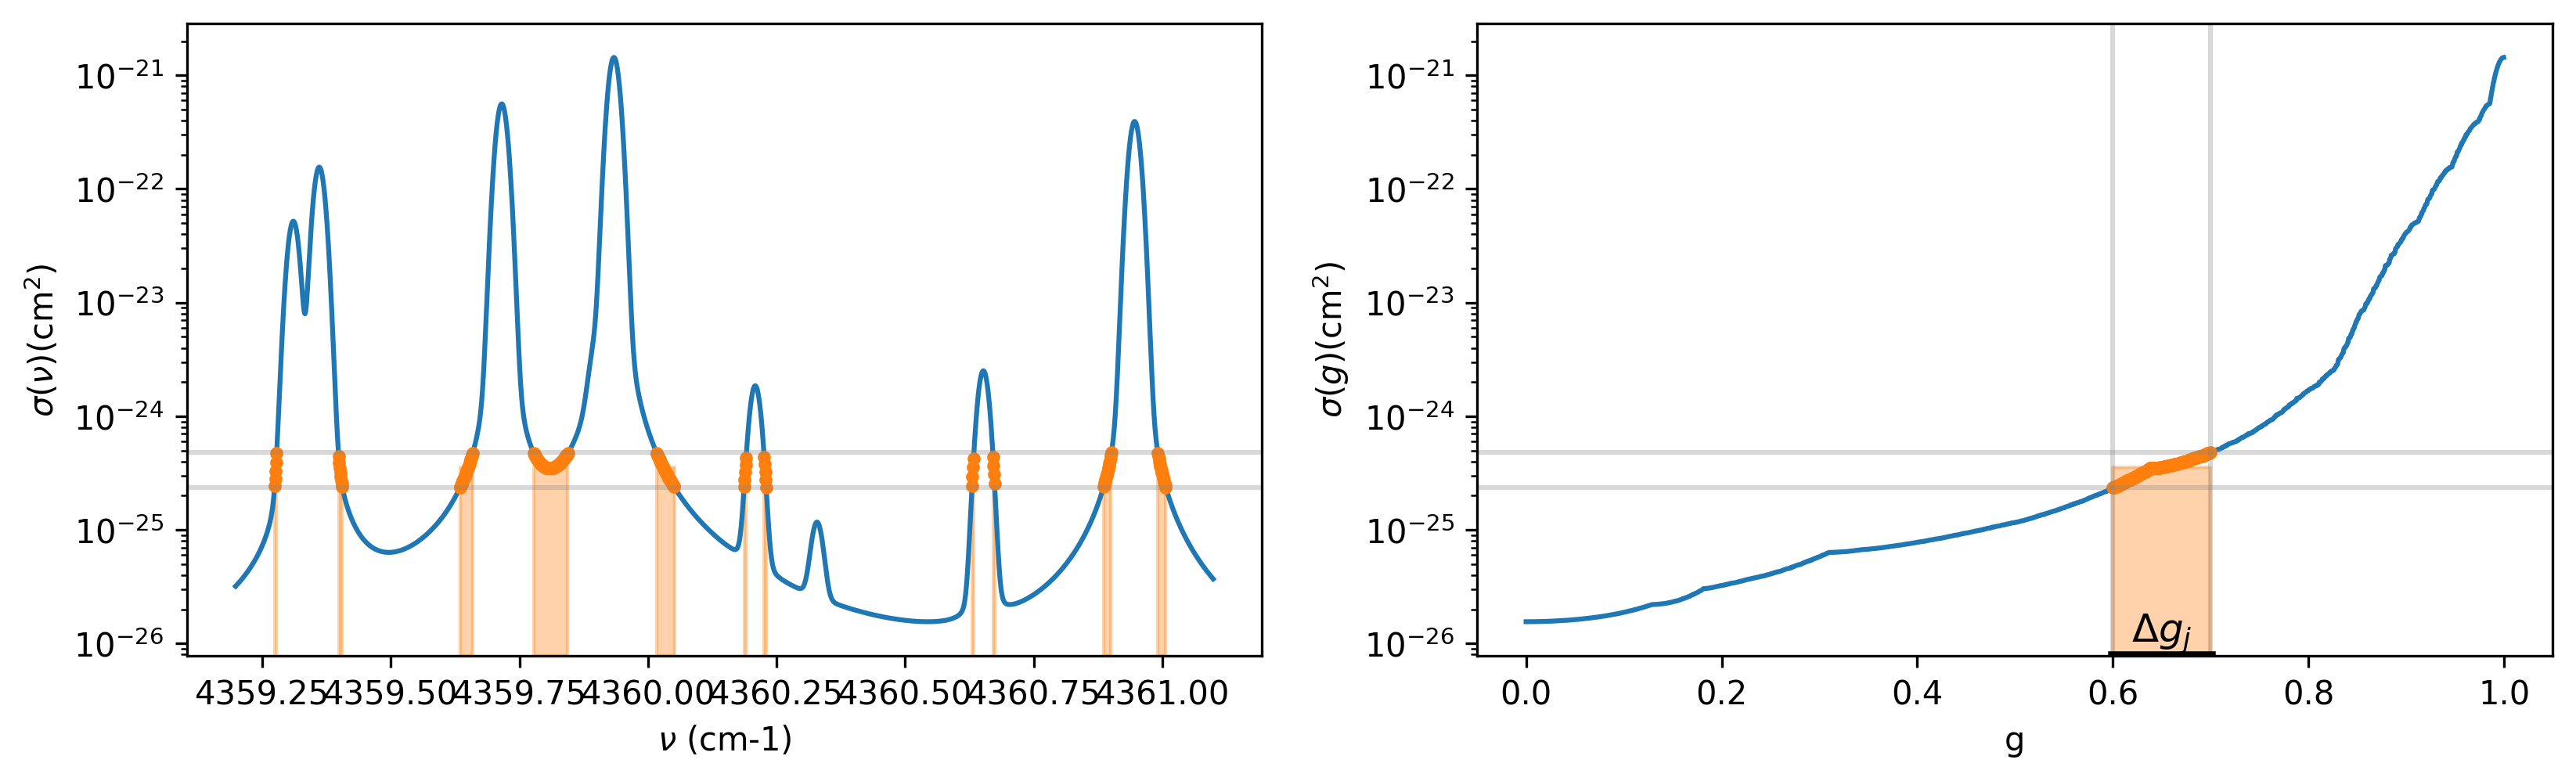
\includegraphics[width=1.0\linewidth]{fig/ckd/corrk_test.png}
    \caption{左:水の断面積を波数空間で示したもの。右:同じ断面積を$g$空間で示したもの。オレンジの領域は$g$空間の$g=0.6-0.7$に属する領域($\Delta g_i$)に含まれる断面積を示している。}
    \label{fig:ckd_fig1}
\end{figure*}


断面積$\sigma(\nu)$(もしくはオパシティ)は、ライン幅より広い波数領域でみると非単射関数、すなわち同じ$\sigma^\prime = \sigma (\nu)$の値をとる$\nu$が複数個存在する(図\ref{fig:ckd_fig1}左)。波長域が広がるにつれ非単射性が増してくる。そこで$\nu$ではなく$\sigma$の値に基づいて情報を記述することが考えられる。たとえば$\sigma(\nu)$の非負値関数である$f(\sigma(\nu)) \geq 0$をある波数幅で積分することを考える。これはリーマン積分では
\begin{align}
 I &= \int_\mathrm{min}^\mathrm{max} f(\sigma(\nu)) d \nu \approx  \sum_i f(\sigma(\nu_i)) \Delta \nu_i
\end{align}
のように、定義域$\nu$方向に分割をして足し合わせる。しかし、非単射性が増してくると、何度も同じような$\sigma$の値について和を取らないとならない。そこで値域の測度に注目して積分を行うことを考える。
いま、値域を互いに重ならない集合に分割する。たとえば$\sigma = \sigma_j$を含む微小領域$\Delta \sigma$内の値域をもつ定義域$\nu$の集合を$A_j$とすると
値域は
\begin{align}
    V = \bigcup_{j=0}^{n} A_j
\end{align}
と表すことができる。集合$A$に関する特性関数
\begin{align}
   \chi_A (\nu) &= \begin{cases}
  1, & \text{if } \nu \in A \\
  0, & \text{if } \nu \notin A
\end{cases}
\end{align}
を用いて、(非負値)単関数
\begin{align}
    s(\nu) = \sum_j^n f_j \chi_{A_j}(\nu)
\end{align}
を考える。ただし $0 \leq f_0 < f_1 < \cdots < f_n$とする。 ルベーグ積分は、集合$A_j$の測度を$m_d (A_j)$としたとき
\begin{align}
    \int_V s(\nu) d \nu = \sum_{j=0}^n f_j \, m_d (A_j)
\end{align}
と定義される。この考えを利用して、積分を行うことを考える。値域の集合として、値域を最小値から最大値までをビニングして、下から順に$j=0,1,\cdots$とする。またそれぞれの集合の代表値を$\sigma_j$とする。$f(\sigma(\nu))$を単関数で
\begin{align}
    f(\sigma(\nu)) \approx s(\nu) = \sum_j^n f(\sigma_j) \chi_{A_j}(\nu)
\end{align}
のように近似することで、
\begin{align}
 \int_V f(\sigma(\nu)) d \nu &\approx \int_V s(\nu) d \nu = \sum_j f(\sigma_j) \Delta m_j \\
 &= (\nu_\mathrm{max} - \nu_\mathrm{min}) \sum_j f(\sigma_j) \Delta g_j 
\end{align}
となる。ここに各集合の測度を$\Delta m_j = (\nu_\mathrm{max} - \nu_\mathrm{min}) \Delta g_j$とおいた。
この最後の式は、(リーマン)積分
\begin{align}
(\nu_\mathrm{max} - \nu_\mathrm{min}) \int_0^1 f(\sigma(g)) dg 
\end{align}
の近似とみることができる。また集合を無限に細かくすれば両者は一致し、
\begin{align}
\label{eq:Lebesgue}
\int_V f(\sigma(\nu)) d \nu = (\nu_\mathrm{max} - \nu_\mathrm{min}) \int_0^1 f(\sigma(g)) dg 
\end{align}
となる。

この$\sigma_j$は値域の小さいほうからビンをとっていて、$\Delta m_j$はこのビンに対応する定義域の測度、つまり定義域の対応する$\nu$空間の長さを表すものであるので、実務的には、$\sigma(g)$は $\sigma(\nu)$を細かく分割したテーブルをソートして、0-1に規格化すれば得られる。図\ref{fig:ckd_fig1}右はそのようにして得られた$\sigma(g)$である。いいかえると$\sigma$の累積分布関数である。ソートであるので単調増加関数となっている。ところでk分布という名前は、この分布関数をopacity ($k$であらわすことが多い)を用いていることに由来していると思われる。

図\ref{fig:ckd_fig1}の塗りつぶし領域は、$f (\sigma) = \sigma$ととった場合の$\Delta g_j$からの寄与を$\nu-f$空間(左)で$g-f$空間(右)で図示したものとなっている。左図で測度$\Delta m_j$は、$\nu$軸で塗りつぶしが被っている領域の和である。これを$(\nu_\mathrm{max} - \nu_\mathrm{min})$で割ったものが右図の$\Delta g_j$に対応する。

$\sigma(g)$がこのようにソートで得られたら、式(\ref{eq:Lebesgue})右辺の評価は通常の数値積分法を利用できる。たとえば、Gauss-Legendre Quadratureなどが用いられる。


\begin{figure*}[!h]
    \centering
    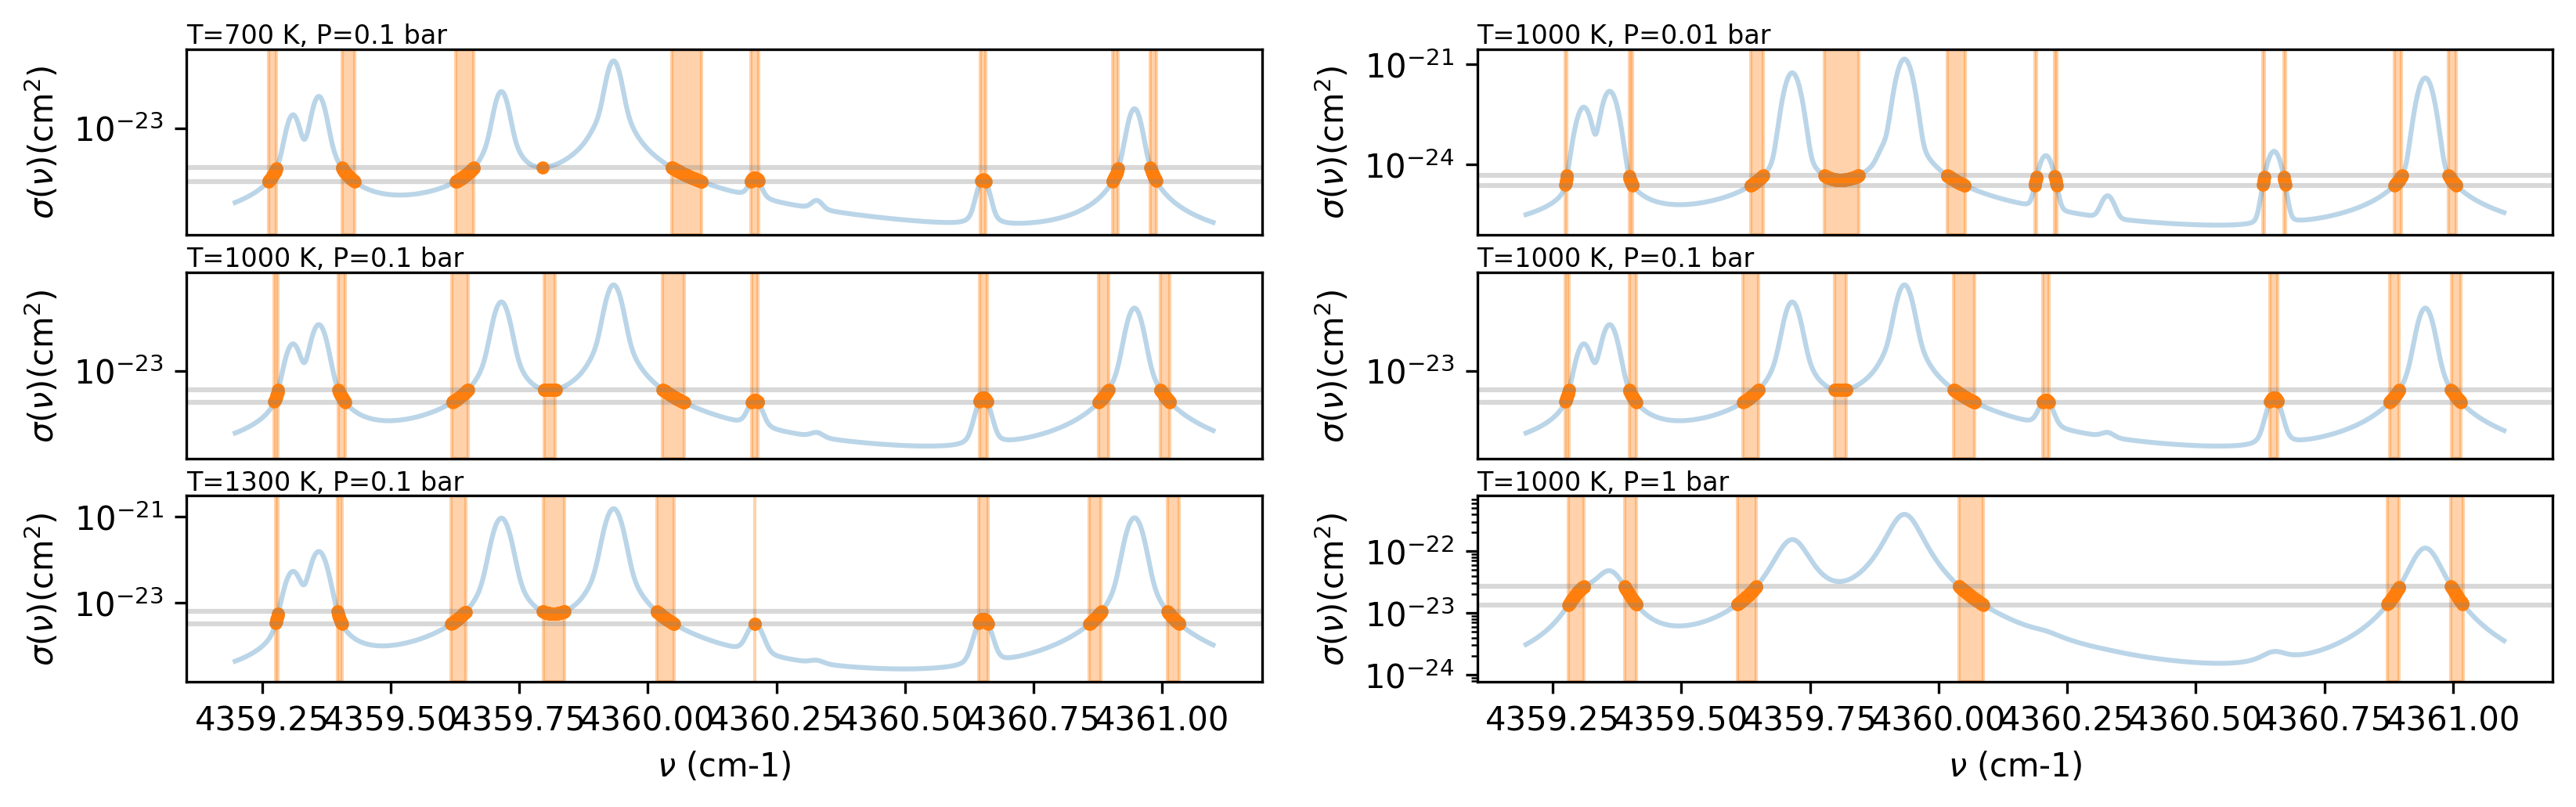
\includegraphics[width=1.0\linewidth]{fig/ckd/corrk_corr.png}
    \caption{左:圧力0.1barで温度を700,1000,1300Kと変えたときに$g$空間の$g=0.6-0.7$に属する領域($\Delta g_i$)に属する断面積をオレンジで示した。この$\delta g_i$は図\ref{fig:ckd_fig1}と同じものを採用している。 右:温度を1000Kに固定し、圧力を0.01,0.1,1barと変更した場合の$\Delta g_i$に属する断面積をオレンジでしめした。}
    \label{fig:ckd_fig2}
\end{figure*}

上では一層の積分を考えたが、放射伝達では各層ごとにオパシティがことなり、これを波数方向で積分する。これを集合$\Delta g_j$ごとの積分に置き換えることができれば、非単射性の強い状況では計算量の削減が期待できる。いいかえると図(\ref{eq:Lebesgue})左のオレンジの部分は、同程度のオパシティとしてまとめて放射伝達を解くことができる。しかしこのためには、各層で$\Delta g_j$に対応する$\nu$の集合が常に一致しないとならない。このような仮定は共単調性(comonotonicity)とよばれ、値域($\sigma$)の順序で並べたときの$\nu$の順序が常に一致していれば、$\Delta g_j$の取り方に寄らず成り立つ。相関k分布法の相関とはこのように層間の共単調性相関を仮定している。これはコピュラではフレシェ・ヘフディング上界を仮定しているのと等しい。

図\ref{fig:ckd_fig2}に温度・圧力を変えたときの$\Delta g_j$を図示する。この例で見るようにラインの中心に関してはだいたい集合が一致しているが、裾になると一致度が悪い。













%\chapter{空間情報の推定}


%\input{mcmc}
%\input{abc}

\footnotesize
\bibliography{ref}{}

\subsection*{教科書類}
ベイズ推定はGelmanらのベイズデータ解析(BDA)、森北出版が定番である。またKevin P. MurphyのProbabilistic Machine Learningはさらに網羅的に重要な事項がまとめられている。




\bibliographystyle{plain}

\end{document}

